\documentclass{book}

\usepackage[a4paper,margin=3cm]{geometry}
\usepackage{cite} % for IEEE-style citations
\usepackage{listings}
\usepackage{xcolor}
\usepackage[hidelinks]{hyperref}
\usepackage{graphicx}
\usepackage{multicol}
\usepackage{subcaption}
\usepackage{fontspec}

%\setmainfont{fonts/TitilliumWeb-Regular.ttf} 
\setmainfont[
%Path = fonts/, % Folder font
UprightFont = TitilliumWeb-Regular, % Format nama font
BoldFont = TitilliumWeb-Bold,
ItalicFont = TitilliumWeb-Italic,
BoldItalicFont = TitilliumWeb-BoldItalic
]{TitilliumWeb}

%\setlength{\parskip}{1em}

\renewcommand{\contentsname}{Daftar Isi}
\renewcommand{\chaptername}{Bab}

% Define Java language style for listings
\lstdefinestyle{JavaStyle}{
	language=Java,
	basicstyle=\ttfamily\footnotesize,
	keywordstyle=\color{blue},
	commentstyle=\color{gray},
	stringstyle=\color{red},
	breaklines=true,
	showstringspaces=false,
	tabsize=2,
	captionpos=b,
	numbers=left,
	numberstyle=\tiny\color{gray},
	comment=[l]{//},
	morecomment=[s]{/*}{*/},
	commentstyle=\color{gray}\ttfamily,
	string=[s]{'}{'},
	morestring=[s]{"}{"},
%	stringstyle=\color{teal}\ttfamily,
%	showstringspaces=false
}

\begin{document}
		
	\begin{titlepage}
		\centering
		\vspace*{1cm}
		
		\Huge
		\textbf{MTI102 - Information System \& Technology Architecture}
		
		\vspace{0.5cm}
		
		\LARGE
		Universitas Pradita
		
		\vspace{1.5cm}
		
		\textit{Powered by ChatGPT}
		
		\vspace{2cm}
		
		\textbf{Alfa Yohannis}
		
		\vspace{0.8cm}
		
		\today
		
		\vfill
	\end{titlepage}
	
	% Contents Page
	\tableofcontents
	
	
	
\chapter{Pengenalan Enterprise Architecture}

\section{Definisi 'Enterprise'}

\subsection{Oxford English Dictionary}
Menurut Oxford English Dictionary, 'Enterprise' didefinisikan sebagai sebuah proyek atau usaha yang biasanya membutuhkan upaya dan keberanian. Selain itu, juga merujuk pada inisiatif, yaitu keberanian untuk mengambil risiko demi mendapatkan keuntungan, serta dapat diartikan sebagai organisasi atau perusahaan bisnis.

\subsection{Cambridge English Dictionary}
Menurut Cambridge English Dictionary, 'Enterprise' merujuk pada kemampuan untuk memikirkan rencana baru dan membuatnya berhasil. Selain itu, istilah ini juga digunakan untuk menggambarkan sebuah perusahaan.

\subsection{Merriam-Webster Dictionary}
Menurut Merriam-Webster Dictionary, 'Enterprise' adalah proyek atau usaha yang sering kali memerlukan keberanian. Definisi ini juga mencakup kesiapan untuk terlibat dalam usaha yang berani dan penuh risiko, serta menggambarkan suatu unit ekonomi yang terorganisir.

\subsection{Kesimpulan Definisi 'Enterprise'}
Secara umum, 'Enterprise' mengacu pada proyek atau usaha yang berani dan penuh risiko. Selain itu, istilah ini juga dapat merujuk pada organisasi atau perusahaan bisnis. Definisi ini secara umum konsisten di antara kamus bahasa Inggris terkemuka.

\section{Definisi 'Arsitektur'}

\subsection{Oxford English Dictionary}
Menurut Oxford English Dictionary, 'Arsitektur' didefinisikan sebagai seni atau praktik merancang dan membangun bangunan. Istilah ini juga dapat merujuk pada gaya atau metode konstruksi serta tata letak atau struktur dari suatu benda.

\subsection{Cambridge English Dictionary}
Menurut Cambridge English Dictionary, 'Arsitektur' adalah seni dan praktik merancang bangunan. Selain itu, istilah ini juga digunakan untuk menggambarkan gaya atau desain dari bangunan tertentu atau sekelompok bangunan, serta cara sesuatu diatur atau disusun.

\subsection{Merriam-Webster Dictionary}
Menurut Merriam-Webster Dictionary, 'Arsitektur' adalah seni atau ilmu dalam merancang dan membangun bangunan. Definisi ini juga mencakup metode atau gaya konstruksi, serta bagaimana bagian-bagian dari suatu objek diatur atau disistematisasi.

\subsection{Ringkasan Definisi 'Arsitektur'}
Secara umum, 'Arsitektur' merujuk pada seni atau praktik merancang dan membangun bangunan. Selain itu, istilah ini juga dapat merujuk pada gaya atau metode konstruksi, serta cara bagian-bagian dari sesuatu diatur atau disistematisasi.

\section{Definisi 'Arsitektur' Menurut IEEE}
Menurut IEEE, 'Arsitektur' adalah organisasi mendasar dari suatu sistem, yang melibatkan komponen sistem dan hubungan antar komponen. Arsitektur juga mencakup manajemen desain dan evolusi sistem, di mana komponen sistem dapat berupa perangkat keras, perangkat lunak, data, orang, dan proses.

\section{Definisi 'Enterprise Architecture'}

\subsection{Menurut Gartner}
Menurut Gartner, 'Enterprise Architecture' adalah disiplin untuk perancangan, perencanaan, pelaksanaan, dan pengendalian proyek. Disiplin ini membantu organisasi mencapai konsistensi antara bisnis dan IT serta melibatkan kolaborasi antara berbagai pemangku kepentingan. 'Enterprise Architecture' juga dapat digunakan untuk membantu dalam pengambilan keputusan strategis.

\subsection{Menurut TOGAF}
Menurut TOGAF, 'Enterprise Architecture' adalah kerangka arsitektur yang memberikan definisi dan desain dasar untuk arsitektur perusahaan. Tujuan dari arsitektur ini adalah untuk memastikan agar operasi perusahaan berjalan secara konsisten dan efisien dengan fokus pada standar dan prosedur yang digunakan di dalam perusahaan.

\subsection{Menurut ISO/IEC/IEEE 42010}
Menurut ISO/IEC/IEEE 42010, 'Enterprise Architecture' adalah pendekatan mendasar terhadap organisasi suatu sistem. Pendekatan ini melibatkan pemahaman semua komponen, hubungan antara komponen, serta lingkungan tempat komponen tersebut beroperasi. Pendekatan ini menekankan pentingnya struktur dan interaksi dalam suatu sistem, serta menyediakan kerangka kerja untuk pemahaman dan desain sistem.

\section{Berbagai Kerangka Arsitektur Enterprise}
Berbagai kerangka arsitektur enterprise telah muncul seiring waktu untuk memandu organisasi dalam menyusun sistem TI dan bisnis mereka. Beberapa kerangka yang terkenal termasuk Business System Planning (BSP), PRISM Architecture Framework, NIST Enterprise Architecture Model, Zachman Framework, Enterprise Architecture Planning (EAP), Sherwood Applied Business Security Architecture (SABSA), dan Federal Enterprise Architecture Framework (FEAF). Kerangka-kerangka ini bertujuan untuk membantu organisasi dalam mengelola kompleksitas sistem mereka, memastikan keselarasan antara tujuan bisnis dan TI.

Kerangka arsitektur enterprise lainnya termasuk Gartner's Enterprise Architecture Method, Department of Defense Architecture Framework (DoDAF), Australian Government AGA, Business Architecture Body of Knowledge (BizBoK), dan ISO Standard for Enterprise Modeling (ISO19439).

\section{Business System Planning (BSP)}
Business System Planning (BSP) melibatkan pemahaman tujuan bisnis, menganalisis proses bisnis, dan merancang arsitektur sistem informasi yang mendukung proses tersebut. BSP membantu organisasi untuk meningkatkan efisiensi, menyederhanakan operasi, dan mengoptimalkan alokasi sumber daya.

\begin{center}
	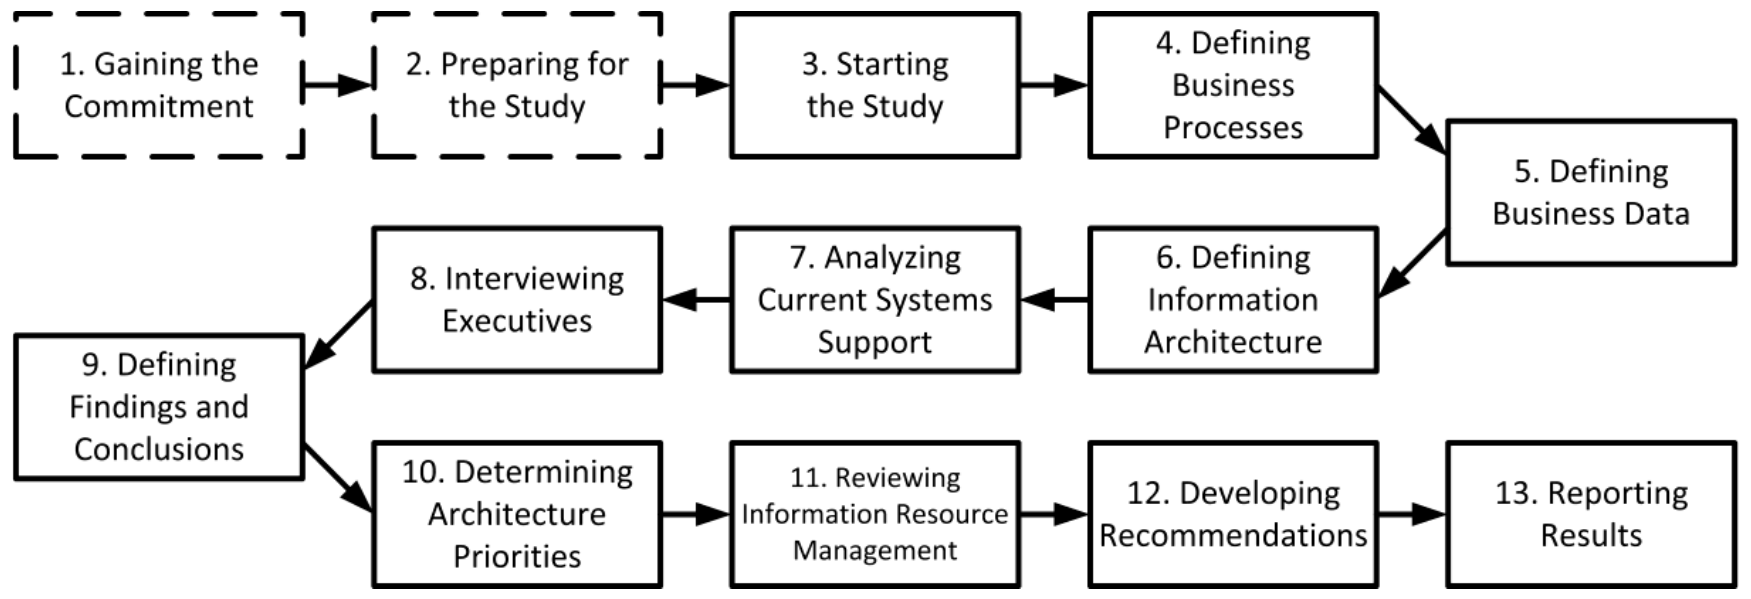
\includegraphics[width=\textwidth]{../figures/bsp}
\end{center}

\section{PRISM Architecture Framework}
PRISM Architecture Framework, atau Partnership for Research in Information Systems Management, merupakan salah satu kerangka arsitektur enterprise yang pertama kali dikembangkan oleh konsorsium vendor TI. Kerangka ini berfokus pada integrasi sistem dan teknologi informasi, membantu organisasi untuk memahami dan mengelola kompleksitas TI.

\begin{center}
	\begin{figure}[ht]
		\begin{minipage}[b]{0.49\linewidth}
			\centering
			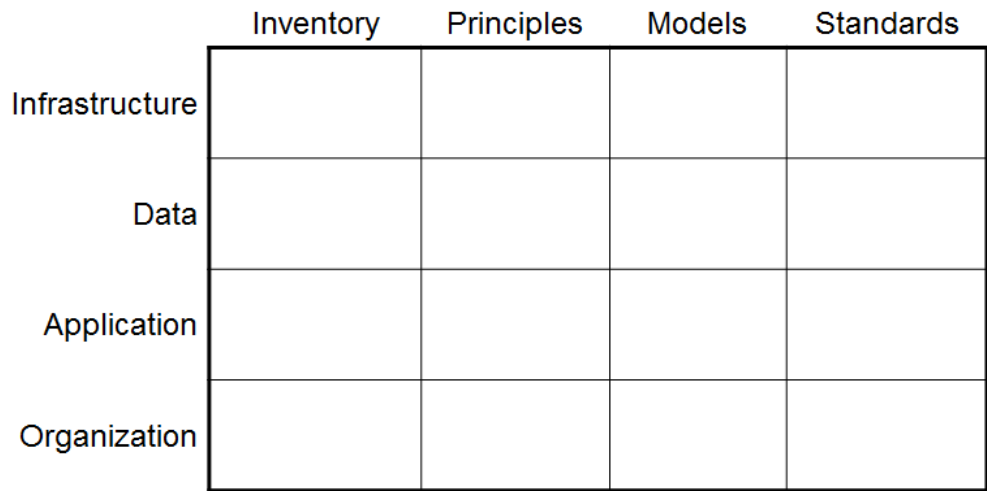
\includegraphics[width=\textwidth]{../figures/prism_matrix}
			\caption{matriks}
		\end{minipage}
		\hfill
		\begin{minipage}[b]{0.49\linewidth}
			\centering
			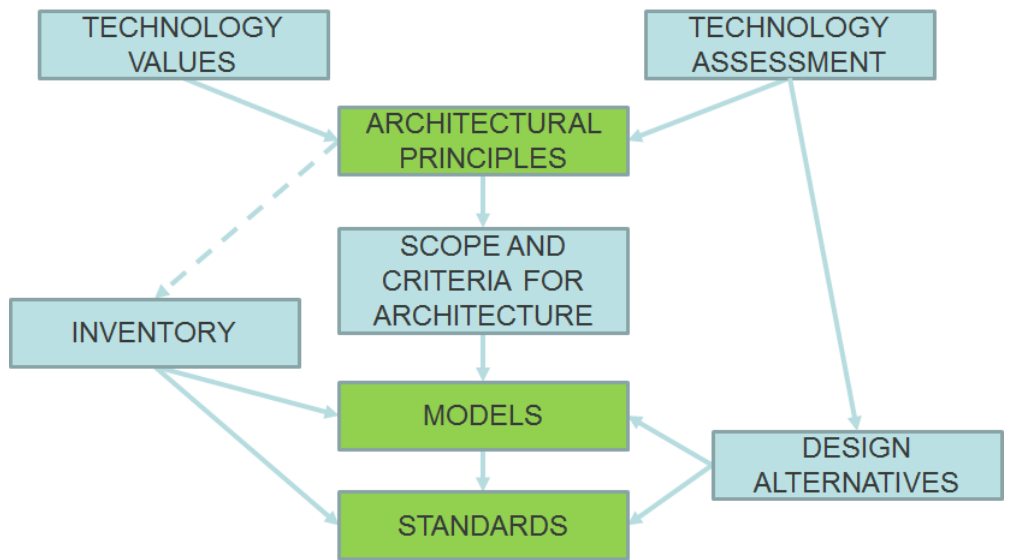
\includegraphics[width=\textwidth]{../figures/prism_relationships}
			\caption{hubungan}
		\end{minipage}
	\end{figure}
\end{center}

\section{NIST Enterprise Architecture Model}
Model Arsitektur Enterprise NIST, yang dikembangkan oleh National Institute of Standards and Technology, menekankan pada pengaturan dan organisasi operasi TI. Model ini membagi arsitektur TI menjadi lima tingkat yang meliputi bisnis, data, aplikasi, teknologi, dan hasil. Ini memungkinkan perencanaan strategis dan pengambilan keputusan berbasis data.

\begin{center}
	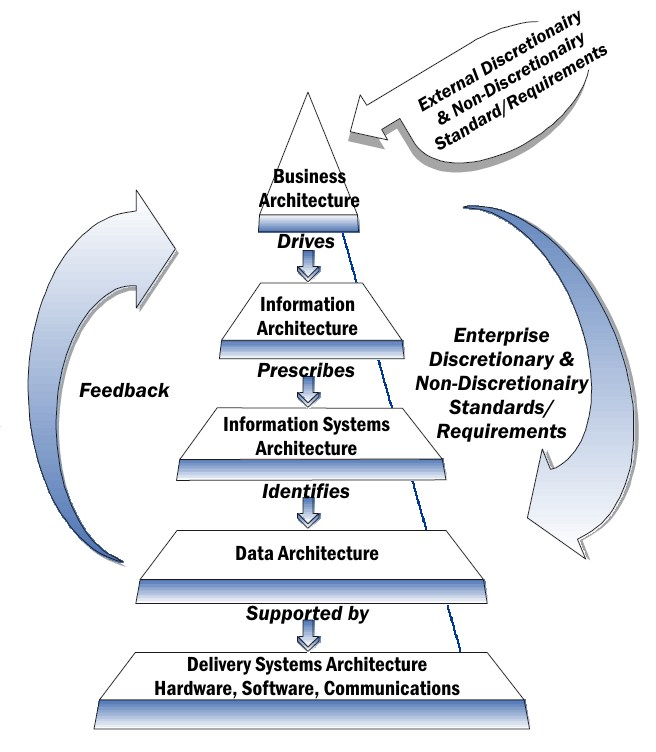
\includegraphics[width=.40\textwidth]{../figures/nist}
\end{center}

\section{Zachman Framework}
Zachman Framework adalah skema untuk memahami dan mengelola kompleksitas arsitektur enterprise, dibagi menjadi enam tingkat berbeda. Framework ini merangkum dari tingkat yang paling abstrak hingga yang paling konkret, cocok untuk berbagai jenis organisasi, dari bisnis hingga pemerintah.

\begin{center}
	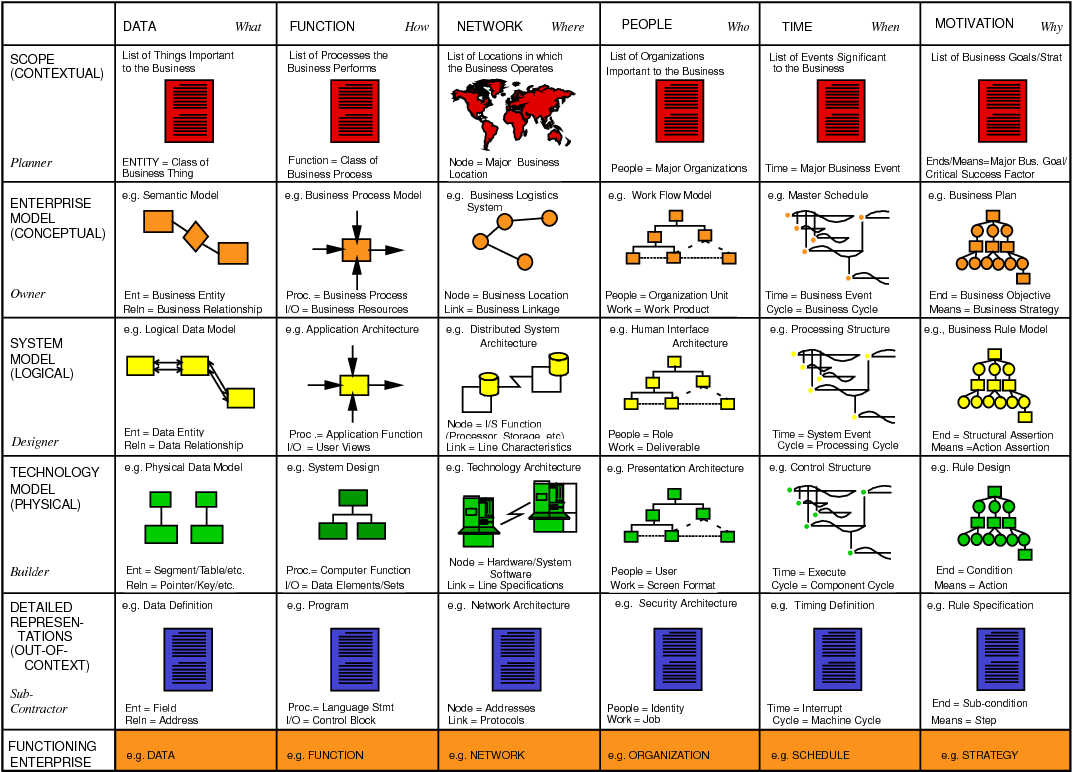
\includegraphics[width=0.76\textwidth]{../figures/zachman}
\end{center}

\section{Enterprise Architecture Planning (EAP)}
Enterprise Architecture Planning (EAP) mencakup metode perencanaan arsitektur sistem informasi. EAP bertujuan untuk mengidentifikasi kebutuhan bisnis dari teknologi informasi dan mengembangkan rencana untuk implementasi teknologi baru berdasarkan kebutuhan tersebut. Ini dapat membantu dalam transformasi digital dan perubahan organisasi.

\begin{center}
	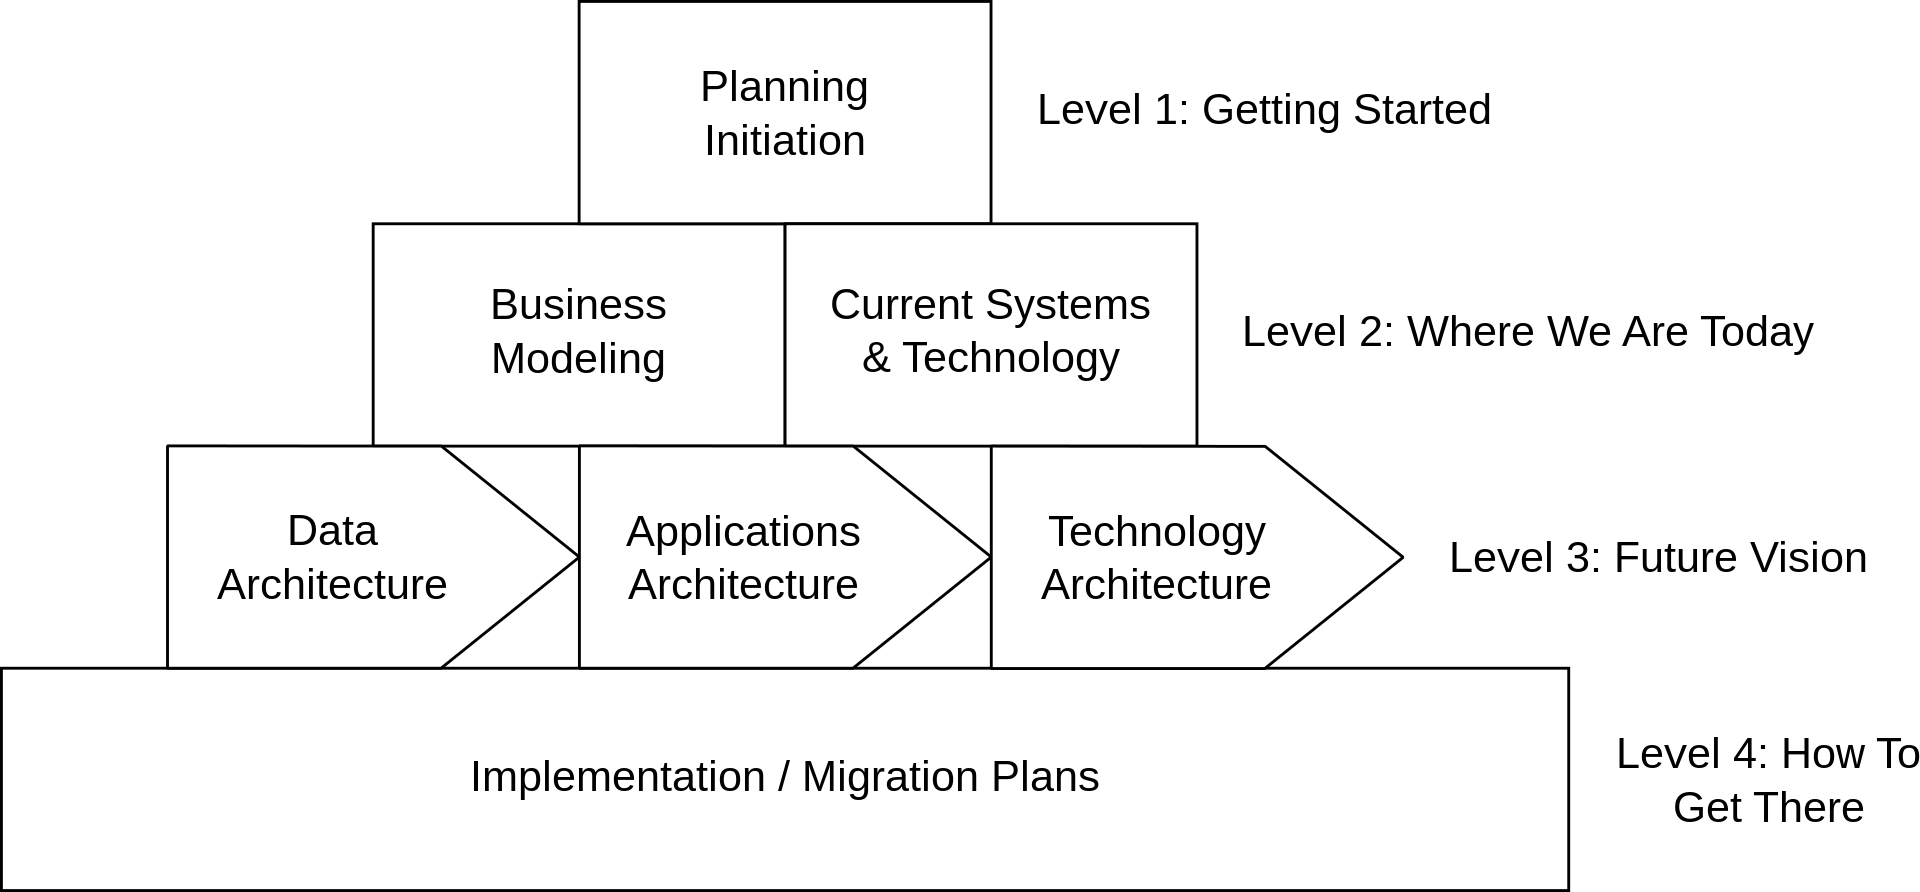
\includegraphics[width=1\textwidth]{../figures/eap}
\end{center}

\section{Sherwood Applied Business Security Architecture (SABSA)}
Sherwood Applied Business Security Architecture (SABSA) menyediakan model dan metodologi untuk mengembangkan kerangka kerja keamanan informasi dan manajemen risiko. SABSA dirancang dengan pendekatan "start-to-finish" dan "top-down" dan dapat disesuaikan dengan kebutuhan spesifik organisasi.

\begin{center}
	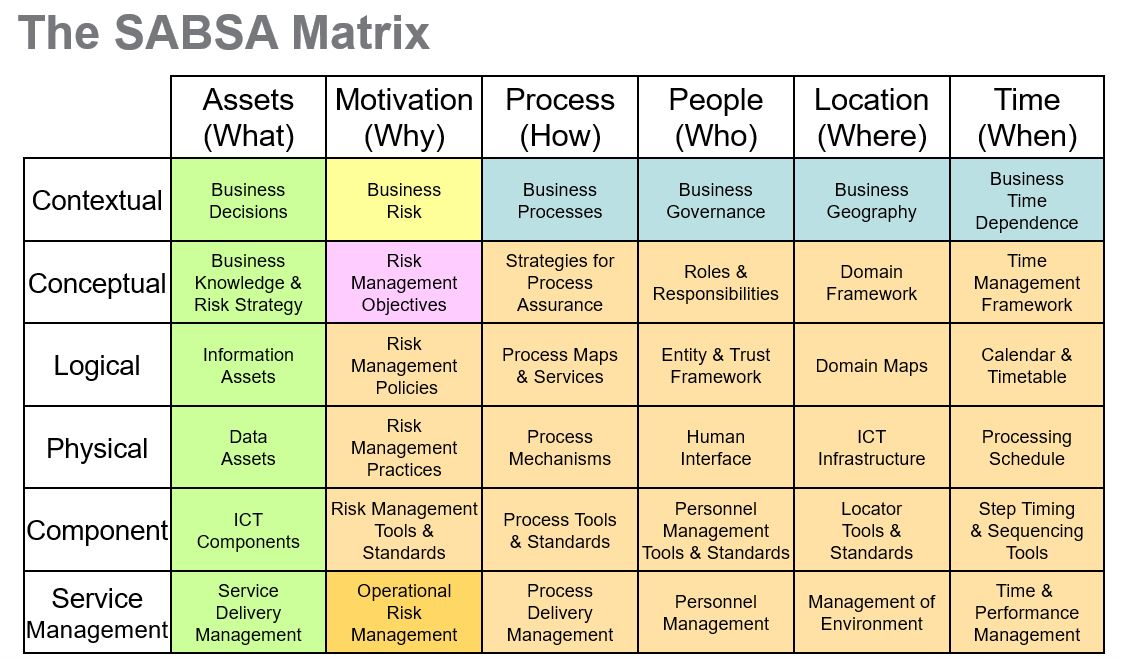
\includegraphics[width=0.8\textwidth]{../figures/sabsa}
\end{center}

\section{Federal Enterprise Architecture Framework (FEAF)}
Federal Enterprise Architecture Framework (FEAF) adalah kerangka kerja yang digunakan oleh pemerintah federal AS. FEAF membantu dalam meningkatkan efisiensi dan efektivitas layanan pemerintah, memfasilitasi kolaborasi antara agen dan departemen pemerintah, dan merupakan bagian dari strategi modernisasi TI pemerintah AS.

\begin{center}
	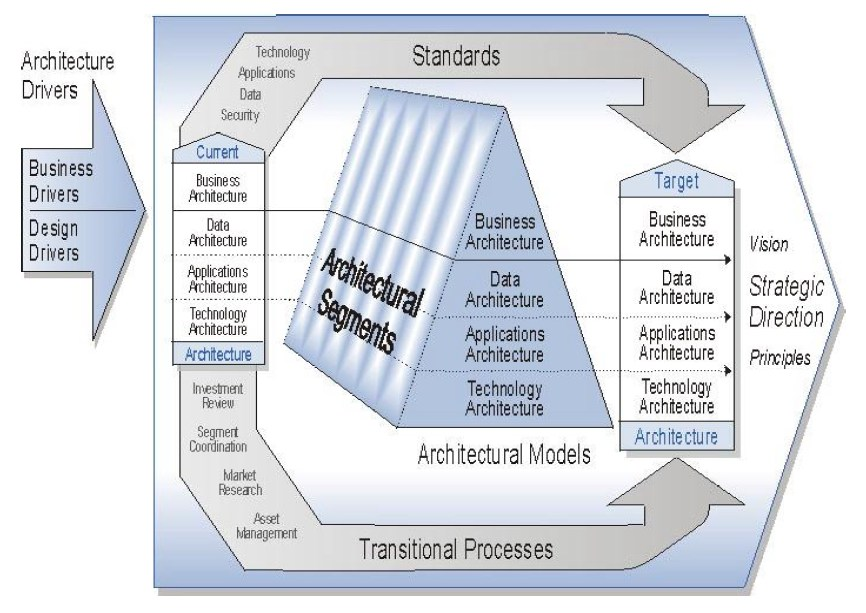
\includegraphics[width=.75\textwidth]{../figures/feaf}
\end{center}

\section{Gartner Enterprise Architecture Method}
Gartner Enterprise Architecture Method dikembangkan oleh perusahaan riset dan konsultasi Gartner. Metode ini membimbing organisasi dalam merancang, mengembangkan, dan menerapkan arsitektur enterprise, menghubungkan strategi bisnis dan TI, serta membantu organisasi mencapai tujuan transformasi digital mereka.

\begin{center}
	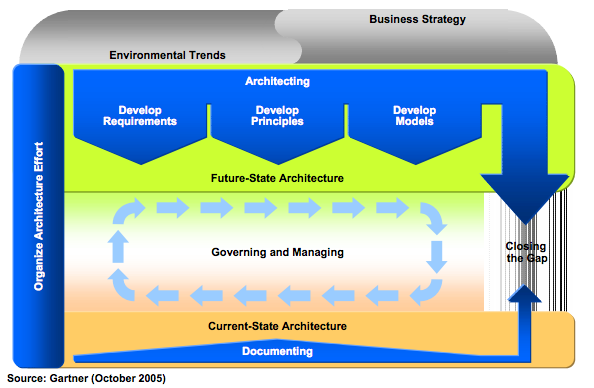
\includegraphics[width=.70\textwidth]{../figures/gartner}
\end{center}

\section{Department of Defense Architecture Framework (DoDAF)}
Department of Defense Architecture Framework (DoDAF) adalah kerangka kerja yang digunakan oleh Departemen Pertahanan AS. Kerangka ini membantu dalam mengorganisir dan memvisualisasikan informasi yang penting untuk proses pengambilan keputusan, menggunakan berbagai model dan panduan untuk mengembangkan arsitektur, dan cocok untuk organisasi dengan kompleksitas dan skala besar.

\begin{center}
	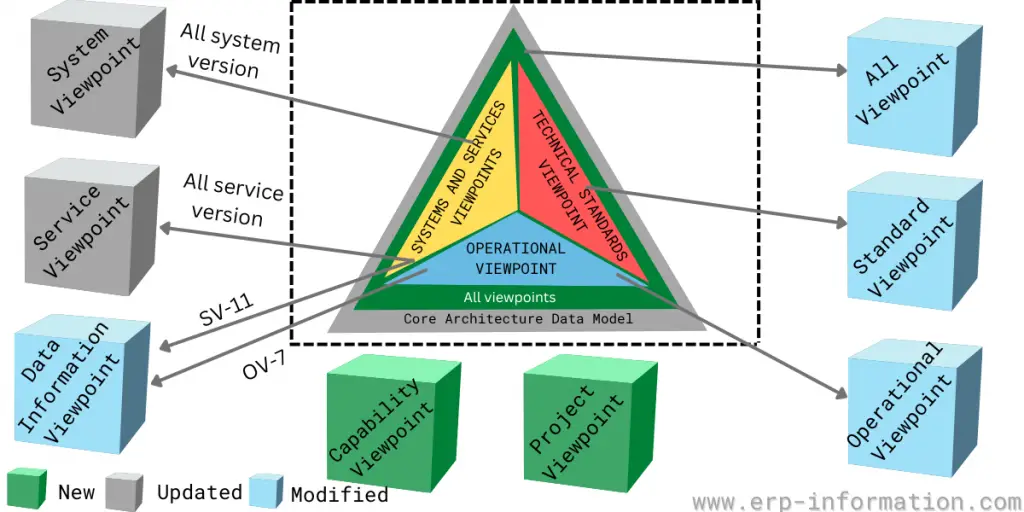
\includegraphics[width=0.68\textwidth]{../figures/dodaf}
\end{center}

\section{Australian Government AGA}
Australian Government AGA adalah kerangka kerja yang digunakan oleh Pemerintah Australia. Kerangka ini membantu dalam perencanaan dan implementasi teknologi informasi di tingkat pemerintah, mendorong kolaborasi antara departemen dan agen pemerintah, serta meningkatkan efisiensi dan transparansi layanan pemerintah.

\begin{center}
	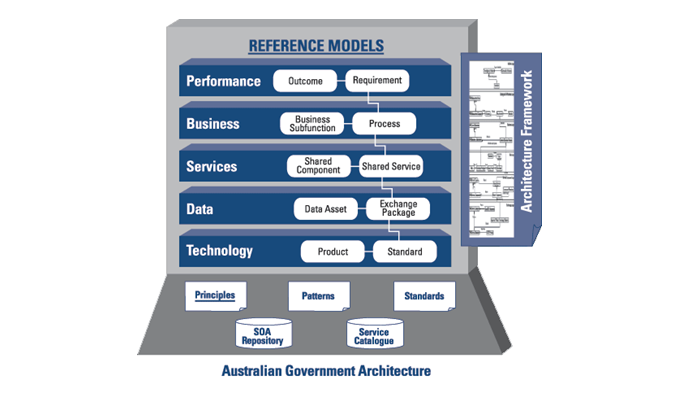
\includegraphics[width=0.9\textwidth]{../figures/aga}
\end{center}

\section{Business Architecture Body of Knowledge (BizBoK)}
Business Architecture Body of Knowledge (BizBoK) adalah panduan yang dikembangkan oleh Business Architecture Guild. Panduan ini menyediakan praktik terbaik dan standar dalam arsitektur bisnis, dapat digunakan oleh arsitek bisnis dan profesional terkait lainnya, serta membantu organisasi dalam merancang dan menerapkan arsitektur bisnis.

\begin{center}
	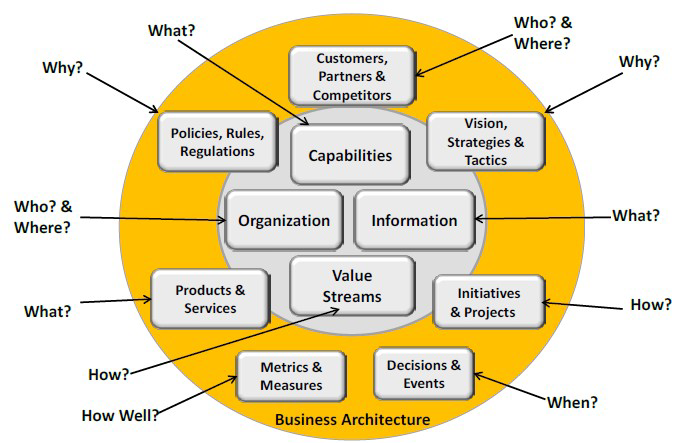
\includegraphics[width=0.7\textwidth]{../figures/bizbok}
\end{center}

\section{ISO Standard for Enterprise Modeling (ISO19439)}
ISO Standard for Enterprise Modeling (ISO19439) adalah standar internasional untuk pemodelan proses bisnis dan organisasi. Standar ini membantu dalam perencanaan, desain, dan perbaikan proses bisnis, dapat digunakan oleh berbagai jenis organisasi, dari bisnis hingga pemerintah, dan dikembangkan oleh Organisasi Internasional untuk Standardisasi (ISO).

\begin{center}
	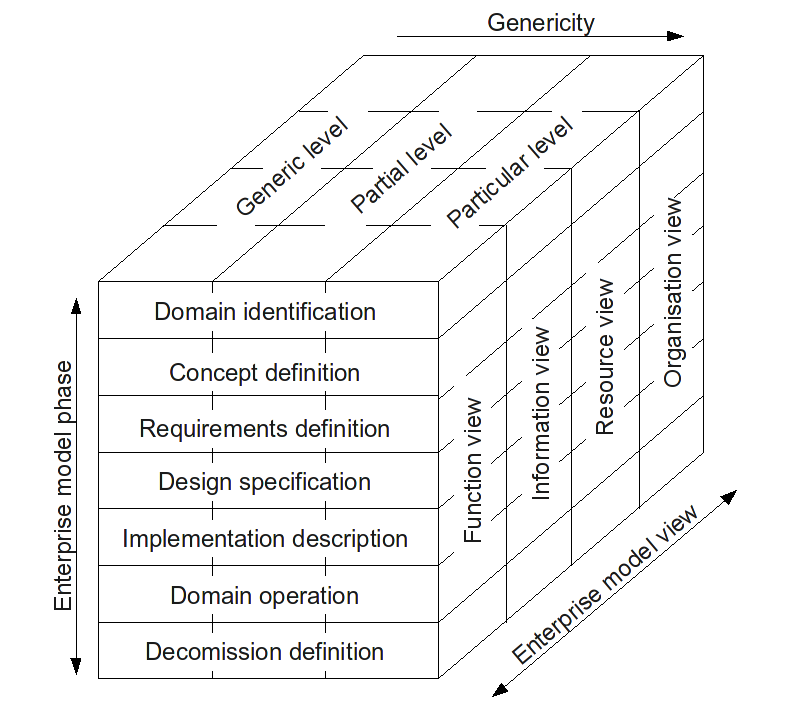
\includegraphics[width=.45\textwidth]{../figures/iso19439}
\end{center}

Terdapat berbagai kerangka dan metodologi arsitektur enterprise yang dapat dipilih sesuai dengan kebutuhan dan konteks spesifik organisasi. Arsitektur enterprise merupakan alat penting untuk perencanaan dan pengelolaan teknologi informasi dalam organisasi.

\section{Kesamaan Antar Kerangka Arsitektur Enterprise}
Meskipun terdapat berbagai kerangka arsitektur enterprise dengan pendekatan dan fokus yang berbeda, beberapa kesamaan mendasar dapat ditemukan di antara mereka:

\begin{itemize}
	\item \textbf{Pendekatan Terstruktur:} Semua kerangka arsitektur enterprise menerapkan pendekatan terstruktur untuk merancang dan mengelola sistem informasi dan TI. Mereka membagi arsitektur menjadi berbagai komponen atau lapisan untuk membantu dalam perencanaan dan implementasi yang lebih baik.
	
	\item \textbf{Fokus pada Keselarasan Strategis:} Kerangka-kerangka ini menekankan pentingnya menyelaraskan teknologi informasi dengan tujuan bisnis organisasi. Mereka berusaha memastikan bahwa keputusan TI mendukung dan memperkuat strategi bisnis keseluruhan.
	
	\item \textbf{Peningkatan Efisiensi dan Efektivitas:} Salah satu tujuan utama dari semua kerangka ini adalah meningkatkan efisiensi dan efektivitas operasional organisasi. Mereka berusaha mengoptimalkan penggunaan sumber daya dan mengurangi kompleksitas dengan memberikan panduan yang jelas dan metodologi yang teruji.
	
	\item \textbf{Manajemen Kompleksitas:} Kerangka-kerangka ini dirancang untuk membantu organisasi dalam mengelola kompleksitas sistem TI dan proses bisnis. Mereka memberikan struktur dan alat untuk memetakan, menganalisis, dan mengelola berbagai aspek arsitektur enterprise.
	
	\item \textbf{Pendekatan Berbasis Model:} Sebagian besar kerangka arsitektur menggunakan model atau representasi visual untuk menggambarkan arsitektur enterprise. Ini membantu dalam memahami hubungan antara berbagai komponen dan bagaimana mereka berinteraksi satu sama lain.
	
	\item \textbf{Fleksibilitas dan Penyesuaian:} Banyak kerangka arsitektur memungkinkan penyesuaian untuk memenuhi kebutuhan spesifik organisasi. Mereka dirancang agar fleksibel dan dapat diterapkan di berbagai konteks dan industri, dari bisnis hingga pemerintahan.
	
	\item \textbf{Penggunaan dalam Perencanaan Strategis:} Kerangka-kerangka ini sering digunakan dalam perencanaan strategis untuk membantu organisasi merumuskan dan mengimplementasikan rencana TI yang selaras dengan tujuan jangka panjang mereka.
\end{itemize}

Dengan kesamaan-kesamaan ini, kerangka arsitektur enterprise memberikan panduan yang kuat untuk organisasi dalam mengelola dan merancang sistem informasi yang efektif dan efisien, meskipun dengan pendekatan dan metode yang berbeda.

\section{Perbedaan Antar Kerangka Arsitektur Enterprise}
Meskipun ada kesamaan di antara berbagai kerangka arsitektur enterprise, perbedaan penting juga ada di antara mereka, yang mencerminkan fokus, metodologi, dan tujuan yang berbeda. Berikut adalah beberapa perbedaan utama:

\begin{itemize}
	\item \textbf{Pendekatan dan Fokus:} Setiap kerangka arsitektur memiliki pendekatan dan fokus yang unik. Misalnya, Framework Zachman menawarkan kerangka kerja berbasis model yang sangat terstruktur untuk manajemen kompleksitas arsitektur, sementara SABSA berfokus pada keamanan dan manajemen risiko dalam konteks arsitektur enterprise.
	
	\item \textbf{Lapisan dan Komponen:} Kerangka arsitektur enterprise dapat memiliki lapisan dan komponen yang berbeda. Sebagai contoh, NIST Enterprise Architecture Model membagi arsitektur TI menjadi lima lapisan yang berbeda, sedangkan Zachman Framework menggunakan enam level berbeda untuk memahami arsitektur dari sudut pandang yang lebih luas.
	
	\item \textbf{Metodologi Pengembangan:} Beberapa kerangka mengikuti metodologi pengembangan tertentu. Misalnya, EAP (Enterprise Architecture Planning) lebih fokus pada perencanaan dan implementasi teknologi baru berdasarkan kebutuhan bisnis, sedangkan Gartner's Enterprise Architecture Method memberikan panduan untuk desain dan implementasi yang berhubungan erat dengan strategi bisnis.
	
	\item \textbf{Penggunaan Model dan Visualisasi:} Setiap kerangka memiliki cara berbeda dalam menggunakan model dan visualisasi. PRISM Architecture Framework, misalnya, menggunakan matriks dan hubungan untuk menggambarkan arsitektur, sementara DoDAF (Department of Defense Architecture Framework) menggunakan berbagai model untuk mendukung proses pengambilan keputusan yang kompleks.
	
	\item \textbf{Aplikasi Sektor dan Konteks:} Beberapa kerangka lebih ditujukan untuk konteks atau sektor tertentu. FEAF (Federal Enterprise Architecture Framework) dirancang khusus untuk pemerintah federal AS, sedangkan Australian Government AGA adalah kerangka kerja yang dirancang untuk meningkatkan efisiensi dan transparansi di tingkat pemerintahan Australia.
	
	\item \textbf{Fleksibilitas dan Penyesuaian:} Derajat fleksibilitas dan penyesuaian juga bervariasi. Beberapa kerangka, seperti Zachman Framework, memiliki struktur yang sangat kaku, terperinci, dan befokus pada artefak, sementara yang lain, seperti SABSA, lebih mudah disesuaikan dengan kebutuhan spesifik keamanan organisasi untuk keperluan bisnis (\textit{business-centric security architectures} dan \textit{risk management frameworks}).
	
	\item \textbf{Standar Internasional:} Kerangka seperti ISO19439 memiliki standar internasional yang mendefinisikan model dan metode untuk perencanaan dan desain proses bisnis, yang mungkin berbeda dengan pendekatan spesifik yang diadopsi oleh kerangka lain.
\end{itemize}

Perbedaan-perbedaan ini mencerminkan variasi dalam kebutuhan organisasi dan konteks di mana kerangka arsitektur diterapkan. Memahami perbedaan ini membantu organisasi memilih kerangka yang paling sesuai dengan tujuan dan tantangan mereka.

\section{Deskripsi Tugas Mata Kuliah Enterprise Architecture}
Untuk membantu kelulusan, mahasiswa diharapkan dapat menghasilkan makalah ilmiah di akhir perkuliahan 1 semester. Model yang dipakailah adalah model flipped classroom di mana mahasiswa akan aktif berpartisipasi dalam perkuliahan. Misalnya, dengan mempresentasikan kemajuan tugas untuk berdiskusi dan mendapatkan umpan balik dari peserta kelas lainnya.

\begin{enumerate}
	\item \textbf{Sesi-01: Introduction to Enterprise Architecture} \\
	\textbf{Tugas}: Identifikasi satu masalah atau peluang di tempat kerja Anda. Anda bisa menggunakan alat-alat analisis seperti SWOT (Strength, Weakness, Opportunity, Threat), Porter's Five Forces, PESTLE (Political, Economic, Social, Technological, Legal, Environmental) ,dsb. Temukan teknologi/inovasi yang dapat meningkatkan kualitas tempat kerja Anda. Identifikasi visi dan misi organisasi tempat Anda bekerja. Wawancarai anggota dewan (\textit{board}), manajer, rekan kerja, atau pihak lain di organisasi tersebut.  Diskusikan ide-ide Anda dengan mereka dan catat umpan balik mereka. Mereka mungkin memberikan ide alternatif atau tambahan. Berdasarkan temuan-temuan ada pada tugas pertemuan sebelumnya, tetapkan \textbf{kemampuan} apa yang perlu ditambahkan ke perusahaan Anda bekerja untuk meningkatkan kualitas bisnisnya. Jadikan itu sebagai studi kasus Anda dan kembangkan arsitektur perusahaan selama semester ini. Ceritakan temuan Anda dalam template makalah.
	
	
	\item \textbf{Sesi-02: Studi Kasus - Remote Working (atau Masalah Lainnya)} \\
	\textbf{Tugas}: 1.) Baca literatur yang membahas TOGAF. 2.) Berdasarkan temuan-temuan ada pada tugas pertemuan sebelumnya, tetapkan \textbf{kemampuan} apa yang perlu ditambahkan ke perusahaan Anda bekerja untuk meningkatkan kualitas bisnisnya. Selanjutlnya, temukan setidaknya 30 sumber pustaka, termasuk makalah akademik, laporan, white papers, dll.
	
	
	\item \textbf{Sesi-03: TOGAF} \\
	\textbf{Tugas}: Lakukan studi literatur terkait visi Anda. Baca setidaknya 30 sumber, termasuk makalah akademik, laporan, white papers, dll., yang sudah Anda kumpulkan sebelumnya.
	
	\item \textbf{Sesi-04: Preliminary Phase} \\
	\textbf{Tugas}: Definisikan visi, yang sering dibagi menjadi tujuan atau sasaran, berdasarkan informasi yang dikumpulkan dalam fase Preliminary. Deskripsikan keadaan saat ini (As-Is) dan keadaan target (To-Be) untuk memperjelas visi tersebut.
	
	\item \textbf{Sesi-05: Phase A - Architecture Vision} \\
	\textbf{Tugas}: Buat model alur kerja/proses bisnis \textbf{As-Is} yang terpengaruh oleh visi. Juga, buat model alur kerja/proses bisnis \textbf{To-Be} yang diperlukan untuk mewujudkan visi tersebut. Identifikasi kesenjangan dan tindakan yang perlu diambil.
	
	\item \textbf{Sesi-06: Phase B - Business Architecture} \\
	\textbf{Tugas}: Buat model data dan dokumen \textbf{As-Is} yang terpengaruh oleh visi dan proses bisnis/workflows As-Is. Selain itu, buat model data dan dokumen \textbf{To-Be} yang diperlukan untuk mewujudkan visi tersebut dan proses bisnis/workflows To-Be. Identifikasi kesenjangan dan tindakan yang diperlukan.
	
	\item \textbf{Sesi-07: Phase C - Data Architecture} \\
	\textbf{Tugas}: Buat model aplikasi \textbf{As-Is} yang terpengaruh oleh visi, proses bisnis/workflows As-Is, dan model data dan dokumen As-Is. Juga, buat model aplikasi \textbf{To-Be} yang diperlukan untuk mewujudkan visi, termasuk proses bisnis/workflows To-Be dan model data dan dokumen To-Be. Identifikasi kesenjangan dan tindakan yang diperlukan.
	
	\item \textbf{Sesi-08: Phase C - Application Architecture} \\
	\textbf{Tugas}: Buat model infrastruktur/teknologi \textbf{As-Is} yang terpengaruh oleh visi, proses bisnis/workflows As-Is, model data dan dokumen As-Is, dan model aplikasi As-Is. Juga, buat model infrastruktur/teknologi \textbf{To-Be} yang diperlukan untuk mewujudkan visi, termasuk proses bisnis/workflows To-Be, model data dan dokumen To-Be, dan model aplikasi To-Be. Identifikasi kesenjangan dan tindakan yang diperlukan.
	
	\item \textbf{Sesi-09: Phase D - Technology Architecture} \\
	\textbf{Tugas}: Kelompokkan tindakan dari sesi sebelumnya ke dalam paket kerja dan estimasikan biaya (termasuk jadwal, tenaga kerja, dan sumber daya lainnya) untuk pelaksanaannya. Identifikasi peluang untuk mengoptimalkan pelaksanaan (misalnya, urutan paket kerja, penggabungan tindakan untuk mengurangi biaya).
	
	\item \textbf{Sesi-10: Phase E - Opportunities and Solutions} \\
	\textbf{Tugas}: Tuliskan semua pekerjaan Anda dan hasilkan makalah akademik (Shinta 2).
	
	\item \textbf{Sesi-11: Phase F - Migration Planning} \\
	\textbf{Tugas}: Tuliskan semua pekerjaan Anda dan hasilkan makalah akademik (Shinta 2).
	
	\item \textbf{Sesi-12: Phase G - Implementation Governance} \\
	\textbf{Tugas}: Tuliskan semua pekerjaan Anda dan hasilkan makalah akademik (Shinta 2).
	
	\item \textbf{Sesi-13: Phase H - Architecture Change Management} \\
	\textbf{Tugas}: Tuliskan semua pekerjaan Anda dan hasilkan makalah akademik (Shinta 2). \textbf{Ubah makalah Anda ke dalam bahasa Inggris.}
	
	\item \textbf{Sesi-14: Requirements Management}. Tidak ada tugas
\end{enumerate}


\section{Aktivitas Kelas dan Tugas}
Identifikasi satu masalah atau peluang di tempat kerja Anda. Anda bisa menggunakan alat-alat analisis seperti SWOT (Strength, Weakness, Opportunity, Threat), Porter's Five Forces, PESTLE (Political, Economic, Social, Technological, Legal, Environmental) ,dsb. Temukan teknologi/inovasi yang dapat meningkatkan kualitas tempat kerja Anda.

Identifikasi visi dan misi organisasi tempat Anda bekerja. Wawancarai anggota dewan (\textit{board}), manajer, rekan kerja, atau pihak lain di organisasi tersebut. Diskusikan ide-ide Anda dengan mereka dan catat umpan balik mereka. Mereka mungkin memberikan ide alternatif atau tambahan. Pilih salah satu sebagai studi kasus Anda dan kembangkan arsitektur perusahaan selama semester ini. Ceritakan temuan Anda dalam template makalah. Template makalah bisa didapatkan di: \url{https://journal.unnes.ac.id/nju/index.php/sji/about/editorialPolicies#focusAndScope}. Klik pada tautan \href{https://docs.google.com/document/d/13pIvz0OUnRtcnNZAcdfQGST5BSpx7LA3/edit}{\textsf{Template Article}}.

	\chapter{Studi Kasus: Kerja Jarak Jauh}

\section{Pendahuluan}

Covid-19 merupakan pemicu utama perdebatan antara Kerja Dari Kantor (WFO) dan Kerja Jarak Jauh. Kontroversi ini berlanjut karena sebagian orang mendukung kerja jarak jauh sementara yang lain menolaknya. Isu ini tetap relevan hingga saat ini, dengan perusahaan-perusahaan yang semakin banyak menerapkan model kerja hybrid. Masalah umum seperti kemacetan lalu lintas, kekhawatiran lingkungan seperti polusi dan perubahan iklim, serta preferensi pekerja berkontribusi pada diskusi yang sedang berlangsung. Masalah kerja jarak jauh adalah isu dunia nyata dengan implikasi yang signifikan.

\section{Penelitian Awal}

Penelitian awal dilakukan di Universitas MTI Pradita, termasuk tugas mahasiswa mengenai topik ini dan survei dengan 91 responden (target: 100). Data tersedia di \url{https://zenodo.org/records/8116799} dan memberikan gambaran tentang masalah kerja jarak jauh. Penelitian ini berguna sebagai dasar untuk menerapkan Arsitektur Perusahaan untuk mengatasi tantangan kerja jarak jauh. Makalah terkait telah dipublikasikan dan dapat diakses di \url{https://ieeexplore.ieee.org/abstract/document/10327330}.

\section{Hasil: Manfaat Kerja Jarak Jauh}

Kerja jarak jauh menawarkan beberapa manfaat:
\begin{itemize}
	\item \textbf{Efektif Biaya}: Mengurangi biaya transportasi bagi karyawan dan biaya operasional bagi perusahaan.
	\item \textbf{Penghematan Waktu}: Waktu perjalanan dialihkan untuk kegiatan lain.
	\item \textbf{Keseimbangan Kerja-Hidup}: Waktu lebih untuk keluarga dan hobi meningkatkan kesehatan mental.
	\item \textbf{Peningkatan Produktivitas}: Fleksibilitas dalam waktu dan tempat meningkatkan hasil kerja dan mengurangi gangguan kantor.
\end{itemize}

\section{Hasil: Tantangan dalam Kerja Jarak Jauh}

Meskipun manfaatnya, kerja jarak jauh menghadapi beberapa tantangan:
\begin{itemize}
	\item \textbf{Jenis Pekerjaan}: Beberapa pekerjaan, seperti pekerjaan pabrik atau penelitian laboratorium, tidak cocok untuk kerja jarak jauh.
	\item \textbf{Masalah Teknis}: Masalah termasuk internet lambat, masalah perangkat keras/perangkat lunak, dan infrastruktur yang tidak memadai.
	\item \textbf{Investasi yang Diperlukan}: Biaya paket data, koneksi internet, dan perangkat keras/perangkat lunak.
	\item \textbf{Isu Etiket}: Tantangan dengan kontak atau tugas di luar jam kerja dan komunikasi yang tidak sopan.
	\item \textbf{Gangguan Lingkungan}: Kondisi rumah yang tidak mendukung mempengaruhi kerja.
\end{itemize}

Tantangan tambahan meliputi:
\begin{itemize}
	\item \textbf{Isu Motivasi}: Karyawan mungkin kekurangan motivasi tanpa pengawasan.
	\item \textbf{Isu Kepercayaan}: Pengawas mungkin meragukan kemampuan karyawan untuk bekerja secara mandiri.
	\item \textbf{Masalah Komunikasi}: Perbedaan dalam kebiasaan komunikasi dibandingkan dengan interaksi langsung.
	\item \textbf{Isu Sosialisasi}: Kesulitan dalam membangun kerja tim dan jaringan.
\end{itemize}

\section{Solusi untuk Tantangan}

Mengatasi tantangan kerja jarak jauh melibatkan beberapa solusi:
\begin{itemize}
	\item \textbf{Solusi Teknis}: Meningkatkan koneksi internet, menyediakan perangkat keras/perangkat lunak, dan memelihara infrastruktur.
	\item \textbf{Sumber Daya Manusia}: Meningkatkan keterampilan non-teknis seperti etiket, kemandirian, motivasi, komunikasi, dan kepercayaan diri. Tingkatkan keterampilan teknis dengan pelatihan penggunaan perangkat lunak dan pemecahan masalah TI.
	\item \textbf{Proses Bisnis dan Tata Kelola}: Sesuaikan proses bisnis untuk kerja jarak jauh. Alihkan penilaian kinerja untuk fokus pada hasil daripada kehadiran atau jam kerja.
\end{itemize}

Solusi tambahan meliputi:
\begin{itemize}
	\item \textbf{Pendanaan}: Kalibrasi ulang dan alokasikan ulang sumber daya keuangan.
	\item \textbf{Interaksi Sosial}: Selenggarakan acara sosial secara rutin untuk mendorong kerja sama, jaringan, dan persahabatan.
	\item \textbf{Infrastruktur dan Dukungan}: Sediakan sumber daya atau bantuan untuk kerja jarak jauh yang efektif.
\end{itemize}

\section{Visi Studi Kasus}
\textbf{Tujuan:} Universitas mampu beroperasi secara fleksibel dengan model kerja hybrid -- Kerja Dari Kantor dan Kerja Dari Mana Saja, dengan \textbf{objektif/target} sebagai berikut:
\begin{enumerate}
	\item Mengubah proses bisnis sesuai dengan tujuan di atas.
	\item Mengubah tata kelola: termasuk pembagian tanggung jawab/wewenang, aturan dalam menilai kinerja sumber daya manusia, dan sebagainya.
	\item Menyiapkan teknologi yang memampukan kerja jarak jauh.
	\item Menyiapkan sumber daya manusia yang siap untuk kerja jarak jauh.
	\item Penyesuaian anggaran untuk mendukung kerja jarak jauh.
\end{enumerate}

%\section{Persyaratan Kelulusan}
%
%Untuk memenuhi persyaratan kelulusan, mahasiswa harus:
%\begin{itemize}
%	\item Menyelesaikan tugas akhir (proyek).
%	\item Menerbitkan satu makalah di jurnal internasional yang terindeks oleh Scopus.
%	\item Menerbitkan dua makalah di jurnal nasional yang terindeks oleh SINTA (platform indeks publikasi nasional).
%	\item Menyajikan dua makalah di konferensi internasional yang terindeks oleh Scopus (misalnya, konferensi IEEE atau ACM).
%\end{itemize}

\section{Aktivitas Kelas dan Tugas}
Berdasarkan temuan-temuan pada tugas pertemuan sebelumnya, tetapkan \textbf{kemampuan} apa yang perlu ditambahkan ke organisasi Anda untuk meningkatkan kualitas bisnisnya. Selanjutnya, temukan setidaknya 30 sumber pustaka, termasuk makalah akademik, laporan, white papers, dll. Ceritakan kemampuan yang Anda temukan di dalam makalah.

\section{Contoh Beberapa Kapabilitas atau Solusi Transisi ke Model Hybrid untuk Kegiatan Kelas dan Perkuliahan}

Seandainya, pihak universitas sepakat untuk mengadopsi model kerja hybrid untuk meningkatkan kualitas dan pengalaman proses belajar mengajarnya, berikut adalah hal-hal yang dapat dilakukan untuk mendukung model kerja tersebut.

\subsection{Platform Pembelajaran dan Teknologi}
\begin{itemize}
	\item \textbf{Platform Pembelajaran Daring:} Gunakan platform pembelajaran daring seperti Moodle, Blackboard, atau Canvas untuk menyampaikan materi kuliah, tugas, dan penilaian. Pastikan platform ini dapat diakses dengan mudah oleh mahasiswa dari berbagai perangkat.
	\item \textbf{Sistem Kelas Virtual:} Implementasikan sistem kelas virtual seperti Zoom, Microsoft Teams, atau Google Meet untuk sesi perkuliahan langsung, diskusi kelompok, dan konsultasi dosen.
	\item \textbf{Alat Pembelajaran Interaktif:} Manfaatkan alat seperti kuis online, polling, dan papan tulis digital untuk meningkatkan keterlibatan mahasiswa selama kuliah.
\end{itemize}

\subsection{Pengajaran dan Kurikulum}
\begin{itemize}
	\item \textbf{Desain Kurikulum Hybrid:} Rancang kurikulum yang mendukung format hybrid dengan kombinasi perkuliahan tatap muka dan online. Tentukan bagian mana yang dapat dilakukan secara daring dan mana yang memerlukan pertemuan langsung.
	\item \textbf{Modul Pembelajaran Asinkron:} Buat modul pembelajaran asinkron yang memungkinkan mahasiswa mengakses materi dan menyelesaikan tugas pada waktu mereka sendiri. Ini mencakup video kuliah, bacaan, dan bahan ajar lainnya.
	\item \textbf{Evaluasi Berkala:} Implementasikan sistem evaluasi berkala yang mencakup kuis online, tugas individu, dan proyek kelompok untuk memantau kemajuan mahasiswa.
\end{itemize}

\subsection{Interaksi dan Keterlibatan}
\begin{itemize}
	\item \textbf{Sesi Tanya Jawab dan Diskusi:} Adakan sesi tanya jawab dan diskusi daring secara rutin untuk menjaga interaksi antara dosen dan mahasiswa. Gunakan breakout rooms dalam platform video untuk diskusi kelompok kecil.
	\item \textbf{Jam Kantor Virtual:} Sediakan waktu jam kantor virtual di mana mahasiswa dapat berkonsultasi langsung dengan dosen melalui video call atau chat.
	\item \textbf{Forum Diskusi:} Gunakan forum diskusi dalam platform pembelajaran untuk memungkinkan mahasiswa bertanya, berdiskusi, dan berkolaborasi secara online.
\end{itemize}

\subsection{Manajemen Kelas}
\begin{itemize}
	\item \textbf{Pendaftaran dan Jadwal Kelas:} Manajemen jadwal kelas dan pendaftaran dapat dilakukan secara daring melalui sistem manajemen akademik untuk memastikan aksesibilitas dan koordinasi yang efektif.
	\item \textbf{Catatan Kehadiran:} Gunakan sistem absensi digital untuk memantau kehadiran mahasiswa pada sesi perkuliahan daring, termasuk integrasi dengan platform pembelajaran untuk kehadiran otomatis.
	\item \textbf{Akses Materi:} Pastikan semua materi kuliah dan bahan ajar dapat diakses oleh mahasiswa melalui platform pembelajaran, dan sediakan salinan materi untuk diunduh jika diperlukan.
\end{itemize}

\subsection{Penilaian dan Umpan Balik}
\begin{itemize}
	\item \textbf{Ujian Online:} Gunakan alat ujian online untuk administrasi ujian yang aman dan terkelola dengan baik. Implementasikan fitur seperti pengacakan pertanyaan dan waktu terbatas untuk menjaga integritas ujian.
	\item \textbf{Umpan Balik Berkelanjutan:} Berikan umpan balik yang cepat dan konstruktif melalui platform pembelajaran atau email, dan dorong mahasiswa untuk memberikan umpan balik mengenai pengalaman pembelajaran daring mereka.
	\item \textbf{Penilaian Otentik:} Terapkan penilaian otentik yang relevan dengan dunia nyata, seperti proyek berbasis kasus atau studi lapangan virtual, untuk mengukur pemahaman dan keterampilan mahasiswa secara lebih holistik.
\end{itemize}

\subsection{Dukungan Teknologi dan Pelatihan}
\begin{itemize}
	\item \textbf{Pelatihan Dosen:} Berikan pelatihan kepada dosen mengenai penggunaan teknologi pembelajaran daring dan strategi pengajaran yang efektif dalam format hybrid.
	\item \textbf{Dukungan TI:} Sediakan dukungan TI yang responsif untuk mengatasi masalah teknis yang dihadapi mahasiswa dan dosen selama sesi perkuliahan daring.
	\item \textbf{Panduan dan Tutorial:} Buat panduan dan tutorial yang jelas untuk mahasiswa mengenai cara menggunakan platform pembelajaran, mengakses materi, dan berpartisipasi dalam kelas virtual.
\end{itemize}

\subsection{Kesejahteraan Mahasiswa}
\begin{itemize}
	\item \textbf{Keseimbangan Kerja-Kuliah:} Dorong mahasiswa untuk menjaga keseimbangan antara studi dan kehidupan pribadi mereka dengan menyediakan fleksibilitas dalam jadwal dan beban tugas.
	\item \textbf{Dukungan Kesehatan Mental:} Sediakan layanan dukungan kesehatan mental secara daring, termasuk konseling dan sumber daya untuk membantu mahasiswa menghadapi stres dan tantangan yang mungkin timbul dari format pembelajaran hybrid.
	\item \textbf{Kegiatan Sosial Virtual:} Selenggarakan kegiatan sosial virtual untuk menjaga keterhubungan mahasiswa dan membangun komunitas meskipun secara daring.
\end{itemize}

\subsection{Data dan Infrastruktur}
\begin{itemize}
	\item \textbf{Manajemen Data:} Gunakan sistem manajemen data berbasis cloud untuk menyimpan dan mengelola data akademik dan administratif secara aman dan terpusat. Pastikan bahwa data mahasiswa, dosen, dan administrasi dapat diakses dengan mudah namun tetap aman.
	\item \textbf{Keamanan Data:} Implementasikan protokol keamanan data yang ketat untuk melindungi informasi sensitif dari akses yang tidak sah. Gunakan enkripsi data dan autentikasi multi-faktor untuk meningkatkan keamanan.
	\item \textbf{Konektivitas Infrastruktur:} Pastikan infrastruktur TI di universitas mendukung konektivitas yang stabil dan cepat untuk mendukung kegiatan pembelajaran daring. Investasikan dalam jaringan yang handal dan redundansi sistem.
\end{itemize}

\subsection{Proses Bisnis Terkait Proses Pembelajaran}
\begin{itemize}
	\item \textbf{Automasi Proses:} Automasi proses administrasi seperti pendaftaran kursus, penilaian, dan pelaporan akademik untuk mengurangi beban kerja administratif dan meningkatkan efisiensi.
	\item \textbf{Integrasi Sistem:} Integrasikan sistem pembelajaran daring dengan sistem manajemen akademik dan keuangan untuk memudahkan koordinasi dan pengelolaan data.
	\item \textbf{Proses Onboarding Mahasiswa Baru:} Rancang proses onboarding yang efisien untuk mahasiswa baru yang mencakup orientasi daring, pelatihan penggunaan platform pembelajaran, dan pengenalan kepada dosen serta staf.
\end{itemize}

	\chapter{Kerangka Arsitektur The Open Group (TOGAF)}

\section{Apa itu Kerangka TOGAF?}

\begin{figure}[h]
	\begin{center}
		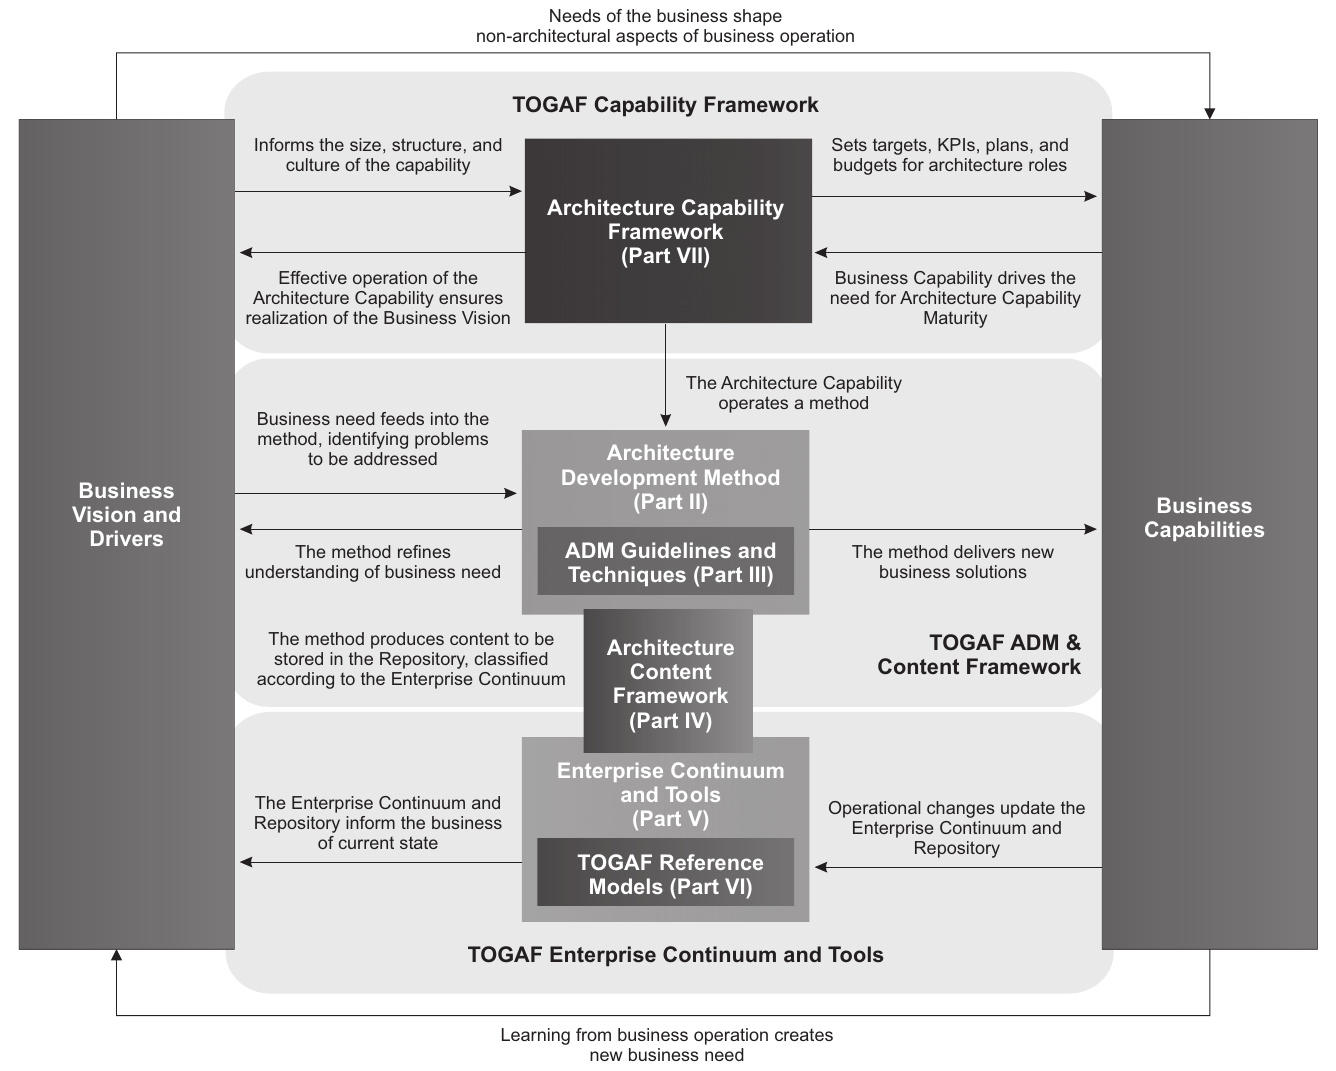
\includegraphics[width=\textwidth]{../figures/togaf}
		\caption{Kerangka Arsitektur The Open Group (TOGAF)}
	\end{center}
\end{figure}

TOGAF adalah sebuah kerangka kerja untuk pengembangan arsitektur perusahaan, yang dikembangkan oleh The Open Group, sebuah konsorsium industri TI. Ini terdiri dari metode dan alat untuk membantu dalam desain, implementasi, dan manajemen arsitektur perusahaan, dengan fokus pada manajemen siklus hidup arsitektur. TOGAF menggunakan pendekatan siklus hidup yang dapat diulang dan iteratif.

\section{Domain Arsitektur}
Kerangka TOGAF mencakup beberapa domain arsitektur: Arsitektur Bisnis berfokus pada strategi bisnis, tata kelola, organisasi, dan proses bisnis utama. Arsitektur Data menangani struktur data logis dan fisik organisasi, serta manajemen data aset dan sumber daya. Arsitektur Aplikasi menyediakan cetak biru untuk sistem aplikasi individu yang akan diterapkan, interaksinya, dan hubungannya dengan proses bisnis inti organisasi. Arsitektur Teknologi mencakup kemampuan perangkat lunak dan perangkat keras yang diperlukan untuk mendukung penerapan aplikasi bisnis, data, dan layanan, termasuk infrastruktur TI, middleware, jaringan, komunikasi, pemrosesan, dan standar.

\section{Komponen TOGAF}
Kerangka TOGAF mencakup berbagai komponen seperti Visi dan Penggerak Bisnis, Kemampuan Bisnis, Kerangka Kemampuan Arsitektur, Metode Pengembangan Arsitektur, dan Pedoman serta Teknik ADM.

Komponen tambahan TOGAF termasuk Kerangka Tata Kelola Arsitektur, Kerangka Konten Arsitektur, Deliverables, Artefak, dan Blok Bangunan, Kontinum dan Alat Perusahaan, serta Repository Arsitektur. Model Referensi TOGAF juga memainkan peran penting dalam mendefinisikan dan membimbing arsitektur perusahaan.

\section{Visi dan Penggerak Bisnis di TOGAF}
Visi bisnis menggambarkan tujuan dan pandangan masa depan sebuah organisasi. Penggerak bisnis adalah faktor yang memicu perubahan dalam sebuah organisasi. TOGAF memanfaatkan visi bisnis dan penggerak untuk membantu mendefinisikan arsitektur perusahaan. Selama fase Preliminary dan Architecture Vision dari ADM, penggerak ini membantu dalam membentuk dan membimbing arsitektur. Penggerak bisnis dapat mencakup perubahan teknologi, pergeseran pasar, atau persyaratan regulasi.

\section{Kemampuan Bisnis di TOGAF}
Kemampuan bisnis adalah kombinasi dari orang, proses, dan teknologi yang memungkinkan sebuah organisasi untuk mencapai tujuannya. TOGAF menganggap kemampuan bisnis sebagai bagian integral dari arsitektur perusahaan. Memahami kemampuan ini membantu dalam merancang dan menerapkan arsitektur yang efektif. Kemampuan bisnis diidentifikasi dan didefinisikan sepanjang proses ADM, membantu dalam desain dan eksekusi arsitektur.

\section{Kerangka Kemampuan Arsitektur TOGAF}
TOGAF 9 menyediakan Kerangka Kemampuan Arsitektur, yang mencakup materi referensi dan pedoman untuk membangun fungsi arsitektur dalam sebuah organisasi. Kerangka ini terdiri dari tujuh kategori: membangun kemampuan arsitektur, dewan arsitektur, kepatuhan arsitektur, kontrak arsitektur, tata kelola arsitektur, model kematangan arsitektur, dan kerangka keterampilan arsitektur. Kategori-kategori ini mencakup kemampuan yang diperlukan untuk menghasilkan arsitektur perusahaan yang efektif dan membantu mengidentifikasi serta mengatasi kekurangan.

\begin{figure}
	\begin{center}
		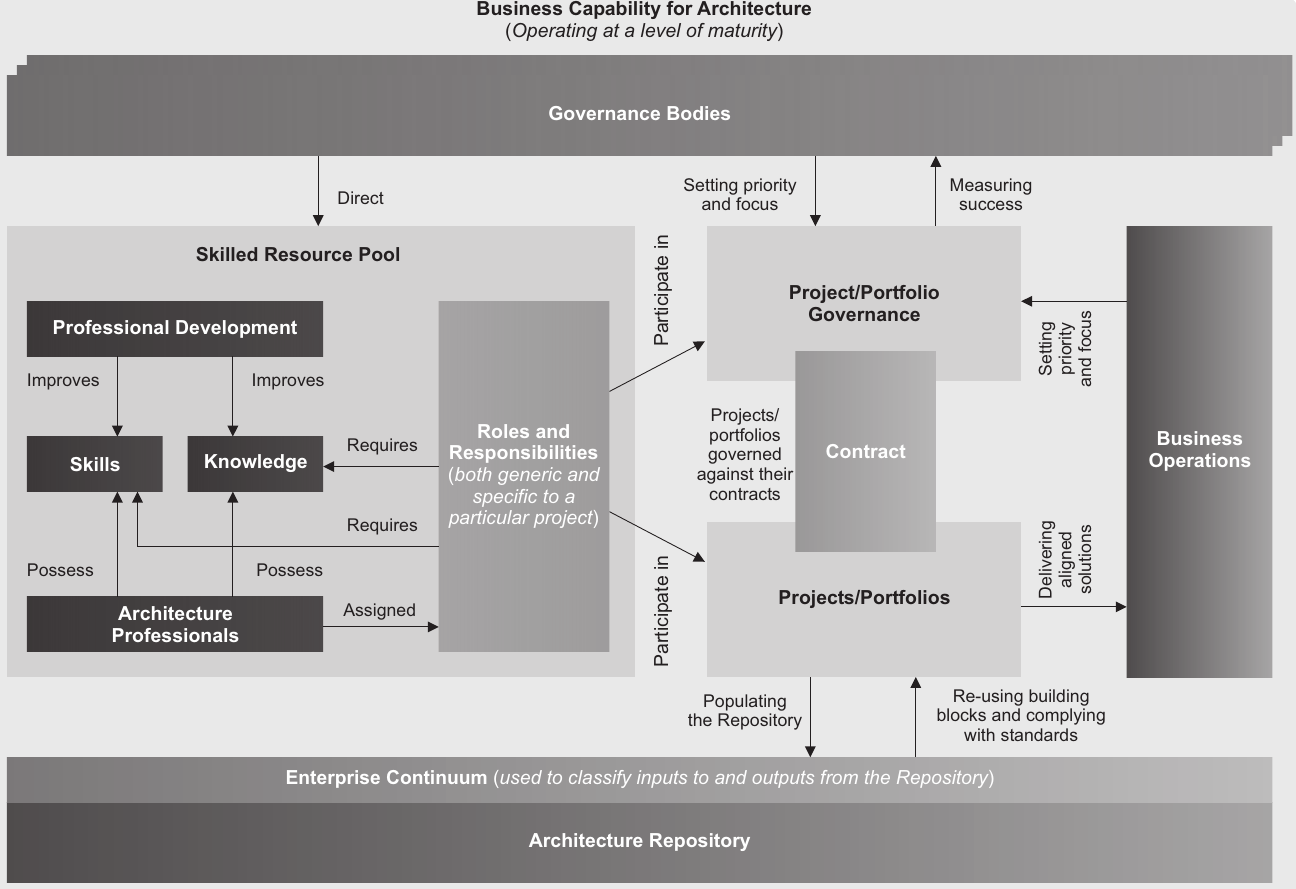
\includegraphics[width=\textwidth]{../figures/architecture_capability_framework}
		\caption{Kerangka Kemampuan Arsitektur}
	\end{center}
\end{figure}

\section{Isi Kerangka Kemampuan Arsitektur TOGAF}
Membuat Arsitektur Kemampuan melibatkan penataan struktur, proses, dan peran untuk mendukung praktik arsitektur organisasi, termasuk cakupan, pemangku kepentingan, dan tata kelola. Dewan Arsitektur mengawasi pembentukan dan operasi Dewan Arsitektur perusahaan. Kepatuhan Arsitektur memastikan bahwa arsitektur organisasi sesuai dengan standar, kebijakan, dan peraturan yang relevan. Kontrak Arsitektur mendefinisikan cakupan, tujuan, dan hasil.

\section{Isi Kerangka Kemampuan Arsitektur TOGAF (2)}
Komponen tambahan dari Kerangka Kemampuan Arsitektur termasuk Tata Kelola Arsitektur, yang memastikan keselarasan arsitektur dengan strategi dan tujuan bisnis. Model Kematangan Arsitektur membantu organisasi menilai dan meningkatkan praktik arsitektur mereka. Kerangka Keterampilan Arsitektur menyediakan peran, keterampilan, dan norma pengalaman untuk pekerjaan arsitektur.

\section{Metode Pengembangan Arsitektur (ADM)}
ADM adalah proses yang direkomendasikan oleh TOGAF untuk mengembangkan arsitektur perusahaan. Ini melibatkan fase yang terorganisir yang membantu dalam merancang, merencanakan, menerapkan, dan mengelola arsitektur perusahaan. Fase-fase ini termasuk Visi Arsitektur, Desain Bisnis, Desain Informasi, Desain Teknologi, dan Implementasi. ADM mengelola seluruh siklus hidup arsitektur perusahaan dan menawarkan pedoman serta teknik untuk setiap fase.

\begin{figure}
	\begin{center}
		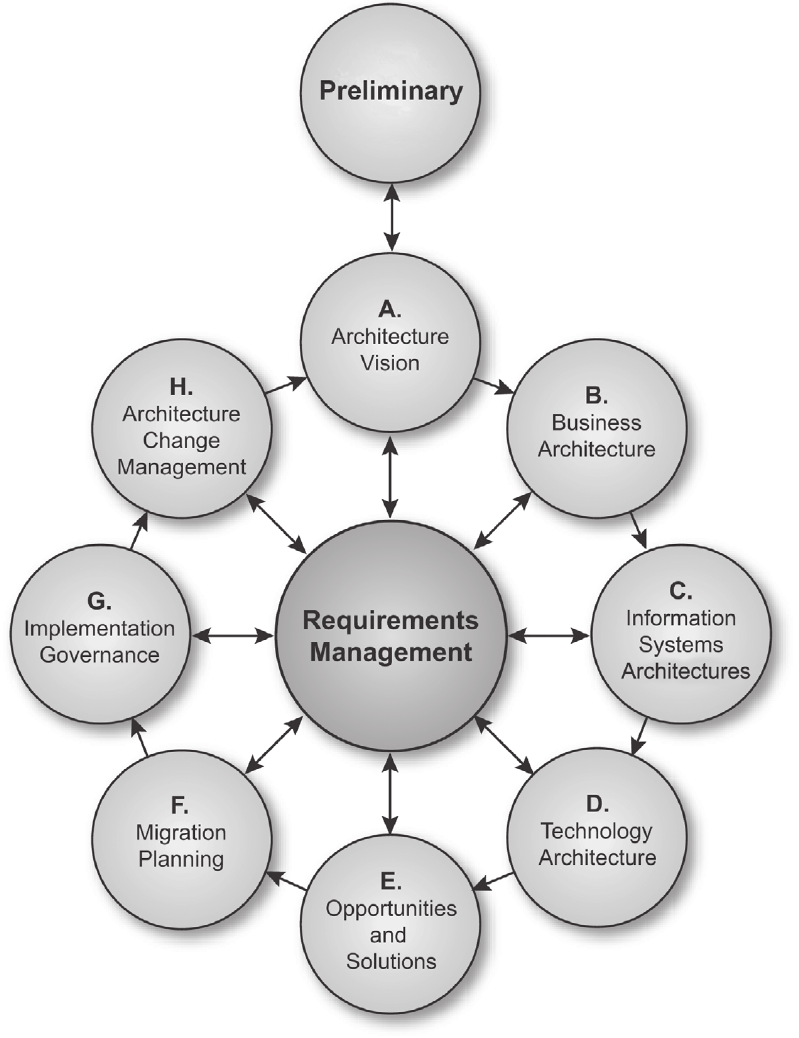
\includegraphics[width=.50\textwidth]{../figures/architecture_development_method}
		\caption{Metode Pengembangan Arsitektur}
	\end{center}
\end{figure}

\section{Pedoman dan Teknik ADM}
TOGAF menyediakan pedoman dan teknik untuk mendukung pelaksanaan ADM. Pedoman ini membantu organisasi menyesuaikan ADM dengan kebutuhan dan konteks spesifik mereka, memastikan proses tetap fokus dan efektif. Teknik umum termasuk analisis prinsip, analisis pemangku kepentingan, analisis kesenjangan, skenario bisnis, rencana migrasi, interoperabilitas, manajemen risiko, dan rencana kemampuan.

\section{Kerangka Tata Kelola Arsitektur}
Tata kelola arsitektur melibatkan pengelolaan dan pengendalian arsitektur perusahaan. TOGAF menyediakan Kerangka Tata Kelola Arsitektur yang mencakup struktur organisasi, peran dan tanggung jawab, proses, dan metode komunikasi. Kerangka ini memastikan bahwa semua proyek selaras dengan arsitektur perusahaan dan strategi bisnis, serta melibatkan pemeliharaan artefak seperti prinsip arsitektur, model, dan peta jalan.

\section{Kerangka Konten Arsitektur}
Kerangka Konten Arsitektur mendefinisikan jenis konten arsitektur yang diperlukan untuk mencakup seluruh domain bisnis. Ini memandu identifikasi, organisasi, dan pengembangan artefak arsitektur. Kerangka ini terdiri dari Deliverables, Artefak, dan Blok Bangunan. Deliverables adalah hasil yang diberikan kepada pemangku kepentingan, Artefak menggambarkan arsitektur, dan Blok Bangunan adalah komponen dari sistem bisnis atau TI.

\section{Deliverables, Artefak, dan Blok Bangunan di TOGAF}
Deliverables adalah hasil pekerjaan arsitektur yang diberikan kepada pemangku kepentingan. Artefak adalah bagian dari Deliverables yang menggambarkan arsitektur secara rinci. Blok Bangunan adalah komponen fisik, logis, atau konseptual dari sistem bisnis atau TI. Contohnya termasuk Dokumen Visi Arsitektur, Diagram Data, dan komponen server atau basis data.

\begin{figure}
	\begin{center}
		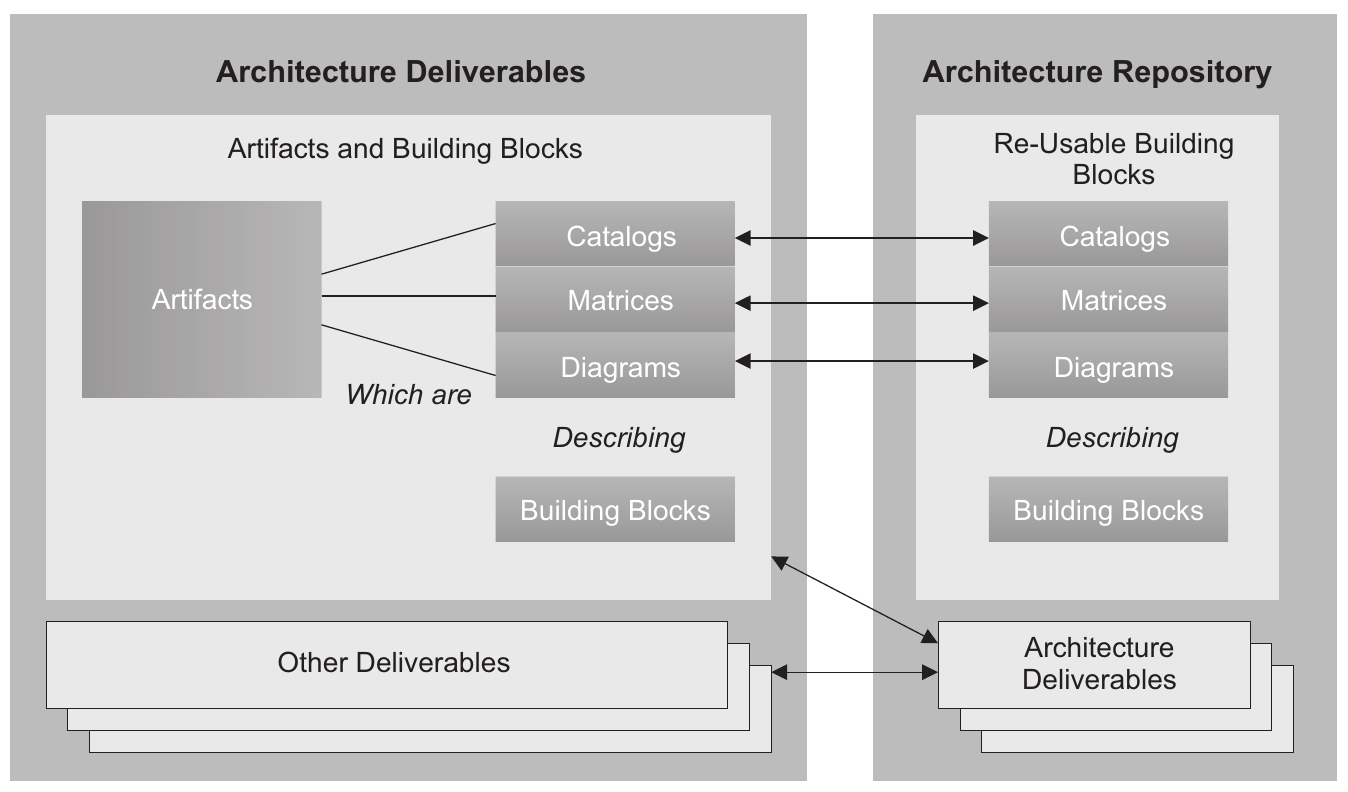
\includegraphics[width=\textwidth]{../figures/architecture_deliverables}
		\caption{Deliverables Arsitektur dan Repository Arsitektur}
	\end{center}
\end{figure}

\section{Kontinum dan Alat Perusahaan}
Kontinum Perusahaan adalah perspektif pada arsitektur dan solusi, mengkategorikan dan mengorganisir artefak. Alat TOGAF membantu dalam membuat, menganalisis, dan mengelola artefak arsitektur, memastikan pekerjaan arsitektur yang efektif dan efisien sepanjang proses ADM.

\section{Repository Arsitektur}
Repository Arsitektur adalah koleksi terstruktur dari artefak arsitektur yang berfungsi sebagai referensi bagi arsitek dan pemangku kepentingan. Ini mencakup prinsip arsitektur, model referensi, dan pola, memastikan bahwa pekerjaan arsitektur terorganisir, konsisten, dan dapat digunakan kembali.

\section{Model Referensi TOGAF}
TOGAF mencakup model referensi untuk membimbing pengembangan arsitektur perusahaan. Model-model ini menyediakan kerangka kerja dan praktik terbaik yang distandarisasi, seperti Model Referensi Teknis TOGAF dan Model Referensi Infrastruktur Informasi Terpadu, membantu memastikan konsistensi dan keselarasan dengan standar industri.

\section{Aktivitas Kelas dan Tugas}
Setelah mengumpulkan 30 literatur, lanjutkan dengan membaca, mengelompokan, dan menyimpulkan makalah-makalah tersebut. Identifikasi apa kontribusi makalah-makalah tersebut terhadap pembangunan Arsitektur Enterprise yang sedang Anda bangun. Identifikasi juga hal-hal apa saja yang membedakan makalah-makalah tersebut dengan kapabilitas Arsitektur Enterprise yang sedang Anda bangun. Tuangkan ke hasil analisis ke dalam makalah.

	\chapter{Fase Awal (\textit{Preliminary})}

\section{Tujuan}
Tujuan dari Fase Awal menentukan spesifikasi kapabilitas arsitektur yang diinginkan (\textit{Desired}) oleh organisasi serta mendefinisikan kapabilitas saat ini (\textit{Current}) dan apa saja yang diperlukan (\textit{Required}) untuk mencapai kapabilitas arsitektur yang dikehendaki. Pada tahap ini, kapabilitas arsitektur dan kebutuhan-kebutuhannya masih bersifat \textit{high-level} dan akan diperinci di fase-fase berikutnya. Tujuan ini dapat dibagi menjadi dua bagian utama:

\subsection{Spesifikasi Kapabilitas Arsitektur yang Diinginkan}
\begin{enumerate}
	\item Meninjau konteks organisasi untuk melakukan arsitektur enterprise.
	\item Mengidentifikasi cakupan bagian dari organisasi enterprise yang terpengaruh oleh Kapabilitas Arsitektur.
	\item Mengidentifikasi kerangka kerja, metode, dan proses yang terkait dengan Kapabilitas Arsitektur.
	\item Menetapkan target Kematangan Kapabilitas.
\end{enumerate}

\subsubsection{Contoh:}

\begin{enumerate}
	\item \textbf{Meninjau konteks organisasi untuk melakukan arsitektur enterprise}
	
	Sebagai langkah awal, universitas perlu meninjau strategi pendidikan yang telah ada dan melakukan evaluasi terhadap model pembelajaran saat ini. Misalnya, universitas mengevaluasi penggunaan ruang kelas fisik, platform e-learning yang sudah tersedia (seperti Learning Management System/LMS), serta kesiapan dosen dan mahasiswa dalam menggunakan teknologi digital. Hal ini mencakup peninjauan fasilitas IT yang ada, kesiapan jaringan internet di kampus, dan kapabilitas sumber daya manusia dalam mendukung pembelajaran hybrid.
	
	\item \textbf{Mengidentifikasi cakupan bagian dari organisasi enterprise yang terpengaruh oleh Kapabilitas Arsitektur}
	
	Mengidentifikasi bagian-bagian dari universitas yang akan terdampak oleh penerapan hybrid teaching and learning. Ini mencakup program studi, dosen, mahasiswa, tim IT, staf administrasi, serta bagian pengelola fasilitas. Contoh cakupan yang terpengaruh adalah perubahan pada metode pengajaran dosen, pelatihan penggunaan LMS untuk dosen dan mahasiswa, serta penyesuaian fasilitas kampus seperti ruang kelas yang dilengkapi dengan perangkat video conference.
	
	\item \textbf{Mengidentifikasi kerangka kerja, metode, dan proses yang terkait dengan Kapabilitas Arsitektur}
	
	Menentukan kerangka kerja dan metode yang akan digunakan untuk mengimplementasikan pembelajaran hybrid. Sebagai contoh, universitas dapat memilih kerangka kerja TOGAF untuk mengelola arsitektur enterprise, ITIL untuk mengelola layanan IT, dan metode ADDIE (Analysis, Design, Development, Implementation, and Evaluation) untuk mengembangkan kurikulum hybrid. Proses-proses yang terkait dapat mencakup pembuatan pedoman penggunaan LMS, kebijakan kehadiran online, serta proses penilaian yang mencakup tugas daring dan luring.
	
	\item \textbf{Menetapkan target Kematangan Kapabilitas}
	
	Menetapkan target kematangan kapabilitas untuk mengukur kesiapan universitas dalam menerapkan pembelajaran hybrid. Sebagai contoh, target kematangan dapat mencakup tingkat integrasi LMS dengan sistem akademik, tingkat adopsi teknologi oleh dosen dan mahasiswa, serta kesiapan infrastruktur IT. Pada tahap awal, target kematangan bisa berupa 50\% dosen menggunakan LMS untuk memberikan materi kuliah, 70\% mahasiswa mampu mengakses dan menggunakan platform hybrid, serta adanya integrasi penuh antara sistem informasi akademik dengan LMS.
\end{enumerate}

\subsection{Mendefinisikan Kapabilitas Saat Ini dan Kebutuhan Apa Saja yang Diperlukan}
\begin{enumerate}
	\item Mendefinisikan Model Organisasi (orang, jabatan, peran, wewenang, departemen terkait, dll.) untuk Arsitektur Enterprise.
	\item Mendefinisikan dan menetapkan proses dan sumber daya secara rinci untuk tata kelola arsitektur.
	\item Memilih dan menerapkan alat yang mendukung Kapabilitas Arsitektur (contoh: Porter’s 5 forces, SWOT, analisis pemangku kepentingan, dll.).
	\item Mendefinisikan prinsip-prinsip arsitektur.
\end{enumerate}

\subsubsection{Contoh:}

\begin{enumerate}
	\item \textbf{Mendefinisikan Model Organisasi (orang, jabatan, peran, wewenang, departemen terkait, dll.) untuk Arsitektur Enterprise}
	
	Dalam konteks hybrid teaching and learning, model organisasi yang perlu didefinisikan melibatkan berbagai peran dan jabatan, seperti:
	\begin{itemize}
		\item \textbf{Dosen dan Staf Pengajar}: Bertanggung jawab dalam menyiapkan materi yang dapat diakses baik secara daring maupun luring.
		\item \textbf{Koordinator Program Studi}: Memastikan bahwa kurikulum dapat diadaptasi ke format hybrid.
		\item \textbf{Tim IT}: Mengelola infrastruktur IT, seperti LMS dan platform video conference, serta memastikan dukungan teknis bagi dosen dan mahasiswa.
		\item \textbf{Departemen Pengembangan Sumber Daya Manusia}: Mengatur pelatihan bagi dosen dan staf pengajar terkait penggunaan teknologi dalam pembelajaran hybrid.
	\end{itemize}
	
	Setiap jabatan perlu memiliki peran dan tanggung jawab yang jelas, seperti dosen yang bertanggung jawab mengunggah materi di LMS setiap minggu atau Tim IT yang melakukan pengecekan infrastruktur daring sebelum setiap semester dimulai.
	
	\item \textbf{Mendefinisikan dan menetapkan proses dan sumber daya secara rinci untuk tata kelola arsitektur}
	
	Proses tata kelola arsitektur untuk pembelajaran hybrid dapat meliputi:
	\begin{itemize}
		\item Prosedur peninjauan kurikulum yang dilakukan oleh koordinator program studi dan dosen untuk memastikan kesesuaian dengan metode pembelajaran hybrid.
		\item Proses eskalasi teknis bagi masalah yang dihadapi oleh dosen atau mahasiswa dalam menggunakan LMS.
		\item Alur kerja pengelolaan konten digital, seperti pengaturan hak akses, upload materi kuliah, dan pengaturan integrasi dengan platform pihak ketiga seperti Zoom atau Google Meet.
	\end{itemize}
	
	Sumber daya yang diperlukan bisa mencakup alat bantu seperti software manajemen kursus, perangkat keras untuk ruang kelas hybrid (kamera, mikrofon, proyektor), serta platform digital untuk asesmen dan evaluasi.
	
	\item \textbf{Memilih dan menerapkan alat yang mendukung Kapabilitas Arsitektur}
	
	Alat yang dipilih harus mendukung proses hybrid teaching and learning. Beberapa contoh alat yang dapat diterapkan adalah:
	\begin{itemize}
		\item \textbf{Learning Management System (LMS)}: Platform seperti Moodle atau Google Classroom untuk mengelola materi kuliah, tugas, dan interaksi antara dosen dan mahasiswa.
		\item \textbf{Alat Video Conference}: Zoom atau Microsoft Teams untuk mendukung kuliah sinkron secara daring.
		\item \textbf{Analisis SWOT dan Pemetaan Pemangku Kepentingan}: Digunakan untuk memahami kekuatan, kelemahan, peluang, dan ancaman dalam penerapan hybrid teaching, serta untuk mengidentifikasi pemangku kepentingan utama yang terlibat.
		\item \textbf{Perangkat Asesmen Daring}: Google Forms atau platform khusus asesmen untuk mengelola ujian, kuis, dan penilaian mahasiswa.
	\end{itemize}
	
	Implementasi alat ini harus sesuai dengan kebutuhan kapabilitas arsitektur, seperti integrasi antara LMS dengan sistem akademik universitas untuk kemudahan pengelolaan nilai dan absensi.
	
	\item \textbf{Mendefinisikan prinsip-prinsip arsitektur}
	
	Prinsip-prinsip arsitektur yang didefinisikan untuk hybrid teaching and learning dapat mencakup:
	\begin{itemize}
		\item \textbf{Prinsip Keterbukaan Akses}: Mahasiswa harus dapat mengakses materi kuliah dan aktivitas pembelajaran dari mana saja dan kapan saja. Hal ini memerlukan desain platform yang user-friendly serta dukungan untuk perangkat mobile.
		\item \textbf{Prinsip Interaksi Sinkron dan Asinkron}: Pembelajaran harus mendukung interaksi secara langsung (live sessions) maupun tidak langsung (materi rekaman dan diskusi forum).
		\item \textbf{Prinsip Kualitas Materi}: Materi pembelajaran harus dapat memenuhi standar akademik, terstruktur, dan mudah dipahami baik dalam format daring maupun luring.
		\item \textbf{Prinsip Keamanan Data}: Menjamin privasi dan keamanan data mahasiswa, dosen, dan staf, terutama ketika menggunakan platform daring dan menyimpan data akademik.
	\end{itemize}
	
	Prinsip-prinsip ini akan menjadi landasan bagi keputusan strategis dan operasional dalam penerapan hybrid teaching and learning, memastikan bahwa setiap langkah yang diambil selaras dengan tujuan arsitektur keseluruhan.
\end{enumerate}



\section{Input}
Input untuk Fase Awal mencakup beberapa dokumen dan kerangka kerja penting:

\begin{itemize}
	\item Kerangka Kerja TOGAF
	\item Kerangka Arsitektur Lainnya
	\item Rencana bisnis, strategi bisnis, dan strategi IT
	\item Prinsip bisnis, tujuan bisnis, dan pendorong bisnis
	\item Kerangka kerja tata kelola dan hukum, termasuk strategi Tata Kelola Arsitektur
	\item Model Organisasi yang ada untuk Arsitektur Enterprise
	\item Kerangka Kerja Arsitektur yang sudah ada, jika ada
\end{itemize}

\subsubsection{Contoh Input yang Digunakan untuk Mendukung Hybrid Teaching and Learning}

\begin{itemize}
	\item \textbf{Kerangka Kerja TOGAF}
	
	TOGAF (The Open Group Architecture Framework) dapat digunakan sebagai panduan untuk mengembangkan kapabilitas hybrid teaching and learning di universitas. Misalnya, universitas dapat menggunakan tahapan dalam TOGAF Architecture Development Method (ADM) untuk mendefinisikan visi arsitektur hybrid, mengidentifikasi kapabilitas yang diperlukan, serta merencanakan implementasi dan pengelolaannya. Kerangka kerja ini membantu dalam merumuskan strategi, merancang model arsitektur, serta memastikan bahwa semua pemangku kepentingan memiliki pemahaman yang sama tentang arah pengembangan kapabilitas hybrid.
	
	\item \textbf{Kerangka Arsitektur Lainnya}
	
	Selain TOGAF, universitas dapat memanfaatkan kerangka kerja lain yang sesuai dengan kebutuhan, seperti Zachman Framework atau Gartner's Enterprise Architecture Framework. Misalnya, Zachman Framework dapat digunakan untuk memetakan komponen-komponen hybrid teaching and learning dalam aspek `What, How, Where, Who, When,` dan `Why`. Ini memungkinkan universitas untuk memahami hubungan antara proses pembelajaran, teknologi yang digunakan, serta peran pemangku kepentingan secara lebih komprehensif.
	
	\item \textbf{Rencana bisnis, strategi bisnis, dan strategi IT}
	
	Rencana bisnis universitas harus sejalan dengan strategi hybrid teaching and learning. Sebagai contoh, jika visi universitas adalah untuk meningkatkan aksesibilitas pendidikan bagi mahasiswa yang berada di luar kota, maka strategi hybrid harus mendukung hal ini dengan menyediakan platform yang dapat diakses dari berbagai lokasi dan perangkat. Selain itu, strategi IT harus mencakup investasi pada infrastruktur seperti cloud computing, sistem informasi akademik, serta platform e-learning yang terintegrasi.
	
	\item \textbf{Prinsip bisnis, tujuan bisnis, dan pendorong bisnis}
	
	Prinsip bisnis universitas yang mendukung hybrid teaching and learning dapat mencakup prinsip `Student-Centric`, di mana setiap keputusan tentang pembelajaran diambil dengan mempertimbangkan pengalaman dan kenyamanan mahasiswa. Tujuan bisnis seperti peningkatan jumlah mahasiswa dari wilayah terpencil atau peningkatan retensi mahasiswa juga menjadi pendorong utama bagi kapabilitas hybrid. Dengan prinsip-prinsip ini, universitas dapat memastikan bahwa setiap perubahan arsitektur sejalan dengan misi dan nilai bisnis.
	
	\item \textbf{Kerangka kerja tata kelola dan hukum, termasuk strategi Tata Kelola Arsitektur}
	
	Kerangka kerja tata kelola seperti COBIT (Control Objectives for Information and Related Technologies) dapat digunakan untuk memastikan bahwa semua inisiatif dalam hybrid teaching and learning dikelola dengan baik, serta memenuhi regulasi dan hukum yang berlaku. Sebagai contoh, universitas harus mematuhi undang-undang perlindungan data pribadi dalam pengelolaan data akademik mahasiswa. Strategi tata kelola arsitektur juga harus mencakup penanganan risiko teknologi serta pengelolaan perubahan dalam kapabilitas hybrid secara berkelanjutan.
	
	\item \textbf{Model Organisasi yang ada untuk Arsitektur Enterprise}
	
	Model organisasi yang sudah ada dapat digunakan sebagai acuan untuk mengembangkan kapabilitas hybrid. Misalnya, jika universitas sudah memiliki struktur departemen IT dan tim akademik, maka dapat ditambahkan peran baru seperti `Hybrid Learning Coordinator` yang bertugas untuk memastikan implementasi dan pengawasan pembelajaran hybrid. Perubahan-perubahan ini perlu dikomunikasikan dengan baik ke seluruh pemangku kepentingan agar ada pemahaman yang jelas tentang tanggung jawab baru.
	
	\item \textbf{Kerangka Kerja Arsitektur yang sudah ada, jika ada}
	
	Jika universitas telah memiliki kerangka kerja arsitektur sebelumnya, misalnya untuk mendukung pembelajaran daring, maka kerangka kerja tersebut dapat disesuaikan dan diperluas untuk mendukung pembelajaran hybrid. Hal ini dapat mencakup penambahan komponen baru pada arsitektur teknologi, seperti integrasi antara ruang kelas fisik dan virtual, serta pengelolaan data interaksi mahasiswa yang mencakup kehadiran dan partisipasi baik secara daring maupun luring.
\end{itemize}

\section{Langkah-Langkah}
Langkah-langkah yang terlibat dalam Fase Awal adalah sebagai berikut:

\begin{enumerate}
	\item Menyusun cakupan organisasi perusahaan yang terkait/terpengaruh.
	\item Memastikan dukungan untuk kapabilitas kerangka kerja arsitektur dan tata kelola yang ditingkatkan.
	\item Mendefinisikan dan membentuk tim arsitektur enterprise dan organisasi.
	\item Mengidentifikasi dan mendefinisikan prinsip-prinsip arsitektur.
	\item Menyesuaikan kerangka kerja TOGAF, \textit{if applicable}, dengan kerangka arsitektur lain yang digunakan.
	\item Menerapkan alat-alat arsitektur.
\end{enumerate}

\subsubsection{Contoh Langkah-langkah dalam Mengembangkan Kapabilitas Hybrid Teaching and Learning}

\begin{enumerate}
	\item \textbf{Menyusun cakupan organisasi perusahaan yang terkait/terpengaruh}
	
	Dalam konteks hybrid teaching and learning di universitas, cakupan organisasi yang terkait meliputi berbagai departemen, fakultas, serta unit pendukung yang memiliki peran penting dalam implementasi pembelajaran hybrid. Misalnya:
	\begin{itemize}
		\item \textbf{Departemen Teknologi Informasi}: Bertanggung jawab terhadap pengelolaan Learning Management System (LMS), infrastruktur jaringan, serta integrasi platform daring seperti Zoom atau Microsoft Teams.
		\item \textbf{Fakultas dan Program Studi}: Terlibat dalam penyusunan kurikulum hybrid, pelatihan dosen, serta pemantauan kualitas pembelajaran.
		\item \textbf{Lembaga Pengembangan Sumber Daya Manusia}: Bertanggung jawab memberikan pelatihan dan workshop bagi dosen terkait metode pengajaran hybrid.
		\item \textbf{Bagian Administrasi dan Keuangan}: Mengatur pengadaan peralatan yang mendukung, seperti perangkat keras untuk ruang kelas hybrid.
	\end{itemize}
	
	Dengan menetapkan cakupan organisasi yang terlibat, universitas dapat memastikan koordinasi dan kolaborasi yang lebih baik antar-departemen dalam penerapan kapabilitas hybrid.
	
	\item \textbf{Memastikan dukungan untuk kapabilitas kerangka kerja arsitektur dan tata kelola yang ditingkatkan}
	
	Universitas harus memastikan bahwa setiap pemangku kepentingan mendukung kapabilitas kerangka kerja arsitektur yang diperbarui. Misalnya, dukungan ini dapat berbentuk alokasi anggaran khusus untuk implementasi sistem pembelajaran hybrid, penyusunan SOP (Standar Operasional Prosedur) baru yang mengakomodasi format hybrid, serta kesediaan manajemen untuk mengadopsi prinsip-prinsip tata kelola arsitektur dalam setiap keputusan strategis terkait pendidikan.
	
	Komunikasi dengan pemangku kepentingan juga menjadi kunci, termasuk dengan dekan, rektorat, dosen, serta mahasiswa, agar setiap pihak memahami manfaat dan peran mereka dalam mendukung kapabilitas hybrid.
	
	\item \textbf{Mendefinisikan dan membentuk tim arsitektur enterprise dan organisasi}
	
	Pembentukan tim arsitektur enterprise khusus untuk hybrid teaching and learning dapat terdiri dari:
	\begin{itemize}
		\item \textbf{Chief Information Officer (CIO)}: Memimpin pengembangan arsitektur IT yang mendukung kapabilitas hybrid.
		\item \textbf{Hybrid Learning Coordinator}: Menjembatani antara kebutuhan akademik dan teknis dalam penerapan pembelajaran hybrid.
		\item \textbf{IT Support Specialist}: Menyediakan dukungan teknis harian, termasuk troubleshooting dan pelatihan penggunaan teknologi.
		\item \textbf{Academic Development Specialist}: Mengawasi penyusunan materi pembelajaran yang dapat diakses baik secara daring maupun luring.
	\end{itemize}
	
	Tim ini bertanggung jawab merencanakan, mengimplementasikan, serta mengevaluasi kapabilitas hybrid untuk memastikan penerapan yang efektif dan efisien di seluruh universitas.
	
	\item \textbf{Mengidentifikasi dan mendefinisikan prinsip-prinsip arsitektur}
	
	Prinsip-prinsip arsitektur yang didefinisikan harus mencakup aspek-aspek penting dari hybrid teaching and learning, seperti:
	\begin{itemize}
		\item \textbf{Konektivitas yang Konsisten}: Menjamin akses internet dan jaringan di seluruh kampus serta memungkinkan mahasiswa untuk bergabung dari lokasi mana pun.
		\item \textbf{Fleksibilitas dalam Pengajaran dan Pembelajaran}: Memastikan bahwa materi kuliah dapat diakses secara sinkron dan asinkron, memberikan fleksibilitas waktu kepada mahasiswa.
		\item \textbf{Keamanan dan Privasi}: Melindungi data pribadi dosen dan mahasiswa, terutama dalam penggunaan platform pembelajaran daring.
	\end{itemize}
	
	Prinsip-prinsip ini akan menjadi panduan bagi setiap keputusan yang diambil dalam proses implementasi kapabilitas hybrid di universitas.
	
	\item \textbf{Menyesuaikan kerangka kerja TOGAF, \textit{if applicable}, dengan kerangka arsitektur lain yang digunakan}
	
	Menyesuaikan kerangka kerja TOGAF untuk mendukung hybrid teaching and learning dapat melibatkan penambahan tahap khusus pada ADM (Architecture Development Method) untuk menangani integrasi antara platform pembelajaran daring dengan sistem informasi akademik yang ada di universitas. Misalnya, universitas dapat menambahkan `Phase G: Implementation Governance` khusus untuk memastikan bahwa setiap perubahan sistem dilakukan sesuai rencana dan standar kualitas yang telah ditetapkan.
	
	Jika universitas juga menggunakan kerangka kerja lain seperti ITIL (Information Technology Infrastructure Library), maka penyesuaian dapat dilakukan pada aspek pengelolaan layanan IT yang mendukung kapabilitas hybrid.
	
	\item \textbf{Menerapkan alat-alat arsitektur}
	
	Alat-alat arsitektur yang diterapkan harus mampu mendukung seluruh proses dan kapabilitas hybrid. Contoh alat yang dapat diterapkan di universitas untuk kapabilitas ini antara lain:
	\begin{itemize}
		\item \textbf{Enterprise Architecture Tools}: Seperti Sparx Enterprise Architect untuk merancang arsitektur hybrid secara komprehensif, mencakup integrasi platform, model data, serta diagram proses.
		\item \textbf{Project Management Tools}: Seperti Jira atau Trello untuk mengelola tugas-tugas terkait implementasi kapabilitas hybrid.
		\item \textbf{Change Management Tools}: Seperti ServiceNow untuk menangani permintaan perubahan yang berkaitan dengan sistem atau teknologi hybrid yang digunakan.
	\end{itemize}
	
	Penerapan alat-alat ini akan membantu universitas dalam merencanakan, melacak, serta mengevaluasi setiap tahap implementasi kapabilitas hybrid, memastikan bahwa semua berjalan sesuai dengan visi dan misi yang telah ditentukan.
\end{enumerate}

\section{Output}
Output dari Fase Awal mencakup item-item berikut:

\begin{itemize}
	\item Model Organisasi untuk Arsitektur Enterprise
	\item Kerangka Kerja Arsitektur yang disesuaikan/diadaptasi, termasuk prinsip-prinsip arsitektur
	\item Repositori Arsitektur Awal
	\item Penegasan kembali atau referensi pada prinsip bisnis, tujuan bisnis, dan pendorong bisnis
	\item Permintaan untuk pekerjaan arsitektur (dokumen resmi)
	\item Kerangka Kerja Tata Kelola Arsitektur
\end{itemize}

\subsubsection{Contoh Output:}

\begin{itemize}
	\item \textbf{Model Organisasi untuk Arsitektur Enterprise}
	
	Dalam konteks `hybrid teaching and learning`, model organisasi untuk arsitektur enterprise harus mencakup peran dan tanggung jawab yang jelas di seluruh departemen dan unit terkait di universitas. Misalnya:
	\begin{itemize}
		\item Pembentukan unit `Hybrid Learning Office` yang berfungsi sebagai pusat koordinasi untuk seluruh kegiatan yang berkaitan dengan pembelajaran hybrid.
		\item Posisi `Hybrid Learning Coordinator` yang memiliki wewenang untuk mengawasi integrasi antara sistem pembelajaran daring dan luring.
		\item Peran `IT Support Specialist` yang bertugas khusus untuk memastikan infrastruktur teknologi selalu siap mendukung kegiatan belajar-mengajar baik secara daring maupun luring.
		\item `Digital Content Specialist` yang membantu dosen dalam mengembangkan materi ajar interaktif, seperti video pembelajaran, kuis daring, serta modul-modul lainnya.
	\end{itemize}
	
	Dengan model organisasi ini, universitas dapat dengan lebih mudah memastikan setiap elemen kapabilitas hybrid dapat dijalankan secara efisien dan terkoordinasi.
	
	\item \textbf{Kerangka Kerja Arsitektur yang disesuaikan/diadaptasi, termasuk prinsip-prinsip arsitektur}
	
	Kerangka kerja arsitektur yang disesuaikan untuk `hybrid teaching and learning` dapat mencakup prinsip-prinsip berikut:
	\begin{itemize}
		\item \textbf{Prinsip Aksesibilitas}: Materi pembelajaran harus dapat diakses oleh semua mahasiswa, baik yang mengikuti kelas secara fisik di kampus maupun secara daring dari lokasi lain.
		\item \textbf{Prinsip Fleksibilitas Pengajaran}: Dosen diberikan kebebasan untuk merancang metode pembelajaran yang paling sesuai, baik menggunakan pendekatan sinkron maupun asinkron.
		\item \textbf{Prinsip Integrasi Sistem}: Semua sistem yang digunakan (Learning Management System, sistem informasi akademik, serta platform video conference) harus dapat saling terhubung dan berbagi data secara efisien.
	\end{itemize}
	
	Penyesuaian prinsip-prinsip ini akan membantu universitas dalam menciptakan lingkungan pembelajaran hybrid yang kohesif dan terintegrasi.
	
	\item \textbf{Repositori Arsitektur Awal}
	
	Repositori arsitektur awal dalam implementasi `hybrid teaching and learning` dapat berupa:
	\begin{itemize}
		\item \textbf{Dokumentasi Infrastruktur Teknologi}: Berisi informasi tentang server, jaringan, serta perangkat keras dan lunak yang digunakan untuk mendukung pembelajaran hybrid.
		\item \textbf{Blueprint Integrasi Sistem}: Menjelaskan bagaimana berbagai sistem di universitas (LMS, sistem informasi akademik, dan lain-lain) saling terhubung.
		\item \textbf{Model Data Pengguna}: Meliputi informasi yang diperlukan untuk mengelola akses pengguna, baik dosen maupun mahasiswa, pada sistem pembelajaran daring dan luring.
	\end{itemize}
	
	Repositori ini menjadi referensi awal yang dapat dikembangkan seiring dengan berkembangnya kapabilitas hybrid di universitas.
	
	\item \textbf{Penegasan kembali atau referensi pada prinsip bisnis, tujuan bisnis, dan pendorong bisnis}
	
	Implementasi `hybrid teaching and learning` harus sesuai dengan prinsip bisnis universitas, tujuan bisnis, serta pendorong bisnis. Misalnya:
	\begin{itemize}
		\item \textbf{Prinsip Bisnis}: Universitas berkomitmen untuk memberikan akses pendidikan yang setara bagi semua mahasiswa, terlepas dari lokasi mereka.
		\item \textbf{Tujuan Bisnis}: Meningkatkan jumlah pendaftaran mahasiswa internasional melalui penyediaan program studi yang dapat diikuti secara hybrid.
		\item \textbf{Pendorong Bisnis}: Meningkatkan fleksibilitas dalam kurikulum untuk menarik lebih banyak mahasiswa dewasa yang ingin belajar sambil bekerja.
	\end{itemize}
	
	Penegasan ini memastikan bahwa kapabilitas hybrid tidak hanya diterapkan dari sisi teknologi, tetapi juga sejalan dengan misi dan visi strategis universitas.
	
	\item \textbf{Permintaan untuk pekerjaan arsitektur (dokumen resmi)}
	
	Contoh dapat dilihat di Subbab \ref{Request for Architectural Work}.
	
	\item \textbf{Kerangka Kerja Tata Kelola Arsitektur}
	
	Kerangka kerja tata kelola arsitektur untuk `hybrid teaching and learning` dapat mencakup elemen-elemen berikut:
	\begin{itemize}
		\item \textbf{Struktur Kepemimpinan}: Membentuk tim tata kelola yang terdiri dari pimpinan IT, pimpinan akademik, serta perwakilan fakultas untuk mengevaluasi penerapan kapabilitas hybrid secara berkala.
		\item \textbf{Prosedur Evaluasi}: Menetapkan prosedur evaluasi dan audit rutin untuk mengukur efektivitas sistem hybrid, baik dari aspek teknis maupun akademis.
		\item \textbf{Mekanisme Eskalasi}: Menyusun mekanisme eskalasi untuk menyelesaikan permasalahan yang muncul selama penerapan kapabilitas hybrid.
		\item \textbf{Dokumentasi dan Pelaporan}: Menyusun dokumentasi hasil evaluasi serta laporan perkembangan kapabilitas hybrid untuk dilaporkan kepada pemangku kepentingan utama.
	\end{itemize}
	
	Kerangka kerja tata kelola ini akan memastikan bahwa kapabilitas hybrid dapat diimplementasikan dengan standar kualitas yang tinggi dan dapat terus dikembangkan sesuai kebutuhan.
\end{itemize}

\section{Mendefinisikan dan Membentuk Tim dan Organisasi Arsitektur Enterprise}
Langkah ini melibatkan pembentukan tim dan mendefinisikan struktur organisasi arsitektur enterprise. Tugas-tugas yang termasuk:

\begin{itemize}
	\item Menentukan kapabilitas perusahaan dan bisnis yang ada.
	\item Melakukan penilaian kematangan arsitektur/perubahan bisnis.
	\item Mengidentifikasi kesenjangan di area kerja yang ada.
	\item Menetapkan peran dan tanggung jawab utama untuk pengelolaan dan pengawasan kapabilitas arsitektur enterprise.
	\item Menulis permintaan perubahan untuk proyek yang ada (dokumen resmi).
	\item Mendefinisikan batasan dalam pekerjaan arsitektur enterprise.
	\item Meninjau dan menyetujui dengan sponsor dan dewan.
	\item Menilai kebutuhan anggaran.
\end{itemize}

\subsubsection{Contoh:}

Langkah ini melibatkan pembentukan tim dan mendefinisikan struktur organisasi arsitektur enterprise yang akan mengelola kapabilitas `hybrid teaching and learning`. Tugas-tugas yang termasuk dalam langkah ini dapat dijelaskan dengan contoh-contoh nyata berikut:

\begin{itemize}
	\item \textbf{Menentukan kapabilitas perusahaan dan bisnis yang ada}
	
	Dalam konteks `hybrid teaching and learning`, universitas perlu meninjau kapabilitas yang dimiliki saat ini, misalnya:
	\begin{itemize}
		\item Apakah universitas sudah memiliki Learning Management System (LMS) yang memadai untuk mendukung pembelajaran daring?
		\item Sejauh mana infrastruktur IT yang ada dapat menampung lonjakan penggunaan platform daring selama jam perkuliahan?
		\item Apakah sumber daya manusia (dosen dan staf) telah memiliki kompetensi yang memadai untuk mengelola pembelajaran hybrid?
	\end{itemize}
	
	Langkah ini akan membantu universitas dalam mengidentifikasi kekuatan dan kelemahan yang ada sebelum memulai pengembangan kapabilitas lebih lanjut.
	
	\item \textbf{Melakukan penilaian kematangan arsitektur/perubahan bisnis}
	
	Penilaian kematangan arsitektur dan perubahan bisnis dilakukan dengan cara menilai kesiapan universitas dalam mengadopsi dan menerapkan model `hybrid teaching and learning`. Contoh nyata dari penilaian ini meliputi:
	\begin{itemize}
		\item Menilai sejauh mana program studi yang ada dapat dikonversi menjadi format hybrid tanpa mengurangi kualitas pembelajaran.
		\item Melakukan survei kesiapan mahasiswa dan dosen dalam menggunakan platform daring sebagai bagian dari kegiatan belajar-mengajar.
		\item Menentukan apakah kebijakan akademik dan administratif mendukung pelaksanaan kegiatan pembelajaran hybrid.
	\end{itemize}
	
	Hasil dari penilaian ini akan menjadi panduan dalam menetapkan prioritas pengembangan kapabilitas.
	
	\item \textbf{Mengidentifikasi kesenjangan di area kerja yang ada}
	
	Identifikasi kesenjangan dilakukan dengan cara membandingkan kapabilitas yang ada dengan kapabilitas ideal yang ingin dicapai. Contoh kesenjangan yang mungkin ditemukan adalah:
	\begin{itemize}
		\item Kurangnya pelatihan bagi dosen untuk membuat materi pembelajaran interaktif yang sesuai dengan platform daring.
		\item Sistem informasi akademik yang belum terintegrasi dengan LMS, sehingga menyulitkan proses pengelolaan nilai dan absensi mahasiswa.
		\item Infrastruktur jaringan yang tidak stabil sehingga menyulitkan akses mahasiswa terhadap materi ajar daring.
	\end{itemize}
	
	Identifikasi kesenjangan ini penting agar universitas dapat menentukan langkah-langkah strategis untuk mengatasi hambatan-hambatan yang ada.
	
	\item \textbf{Menetapkan peran dan tanggung jawab utama untuk pengelolaan dan pengawasan kapabilitas arsitektur enterprise}
	
	Dalam penerapan `hybrid teaching and learning`, menetapkan peran dan tanggung jawab yang jelas sangatlah penting. Contoh penetapan peran meliputi:
	\begin{itemize}
		\item \textbf{Hybrid Learning Coordinator}: Bertanggung jawab dalam memastikan semua kegiatan pembelajaran hybrid berjalan lancar, mengatasi kendala yang muncul, dan menjadi penghubung antara dosen dan tim IT.
		\item \textbf{Instructional Designer}: Berperan untuk membantu dosen dalam merancang materi ajar yang sesuai dengan metode hybrid, baik untuk pembelajaran sinkron maupun asinkron.
		\item \textbf{Technical Support Specialist}: Menyediakan dukungan teknis untuk dosen dan mahasiswa, terutama dalam penggunaan LMS, sistem video conference, serta perangkat keras dan lunak lainnya.
	\end{itemize}
	
	Penetapan peran ini memastikan adanya pembagian tanggung jawab yang jelas, sehingga kapabilitas hybrid dapat dikelola dengan lebih efisien.
	
	\item \textbf{Menulis permintaan perubahan untuk proyek yang ada (dokumen resmi)}
	
	Jika kapabilitas `hybrid teaching and learning` akan mempengaruhi proyek-proyek yang sedang berjalan di universitas, diperlukan permintaan perubahan resmi. Contoh dokumen yang dapat disusun:
	\begin{itemize}
		\item Permintaan perubahan untuk menyelaraskan proyek pengembangan kurikulum dengan strategi hybrid.
		\item Permintaan perubahan untuk pengembangan infrastruktur IT yang mendukung platform daring dan luring secara terintegrasi.
		\item Permintaan perubahan untuk menyediakan anggaran tambahan guna pelatihan dosen dalam memanfaatkan platform hybrid.
	\end{itemize}
	
	Dokumen ini harus disusun secara rinci dan disetujui oleh pihak-pihak yang terkait, seperti manajemen fakultas dan divisi IT.
	
	\item \textbf{Mendefinisikan batasan dalam pekerjaan arsitektur enterprise}
	
	Dalam kapabilitas `hybrid teaching and learning`, mendefinisikan batasan kerja penting untuk menghindari konflik tanggung jawab dan memastikan fokus pada tujuan utama. Contoh batasan dapat meliputi:
	\begin{itemize}
		\item Batasan pada pengembangan konten hanya untuk mata kuliah yang secara formal terdaftar dalam kurikulum hybrid.
		\item Batasan tanggung jawab IT Support Specialist hanya pada permasalahan teknis dan tidak mencakup pelatihan materi ajar.
		\item Batasan akses pada sistem informasi bagi mahasiswa hanya pada jam-jam tertentu untuk memastikan stabilitas server.
	\end{itemize}
	
	Batasan-batasan ini perlu didefinisikan dengan jelas agar setiap pihak yang terlibat memahami lingkup pekerjaan masing-masing.
	
	\item \textbf{Meninjau dan menyetujui dengan sponsor dan dewan}
	
	Sebelum kapabilitas `hybrid teaching and learning` diimplementasikan, perlu ada persetujuan resmi dari sponsor (pihak yang mendanai proyek) dan dewan universitas. Proses ini dapat meliputi:
	\begin{itemize}
		\item Presentasi strategi dan rencana implementasi kapabilitas hybrid kepada sponsor dan dewan.
		\item Diskusi mengenai alokasi sumber daya (dana, tenaga kerja, infrastruktur) yang diperlukan.
		\item Persetujuan atas rencana kerja dan penetapan milestone yang harus dicapai.
	\end{itemize}
	
	Persetujuan ini akan memastikan bahwa seluruh pemangku kepentingan memiliki pemahaman yang sama dan mendukung penuh pelaksanaan kapabilitas hybrid di universitas.
	
	\item \textbf{Menilai kebutuhan anggaran}
	
	Penilaian kebutuhan anggaran dilakukan dengan memperkirakan biaya yang dibutuhkan untuk penerapan kapabilitas `hybrid teaching and learning`. Contoh perhitungan anggaran dapat mencakup:
	\begin{itemize}
		\item Biaya pengembangan infrastruktur IT (server, jaringan, lisensi perangkat lunak).
		\item Biaya pelatihan dan pengembangan kompetensi dosen.
		\item Biaya pemeliharaan dan dukungan teknis selama periode implementasi awal.
		\item Biaya pengembangan materi ajar digital, seperti video pembelajaran, modul interaktif, dan lain-lain.
	\end{itemize}
	
	Estimasi anggaran ini akan menjadi acuan bagi manajemen universitas dalam menyusun rencana pembiayaan yang realistis dan sesuai kebutuhan.
\end{itemize}

\section{Contoh Prinsip-Prinsip Arsitektur}
Berikut adalah beberapa contoh prinsip arsitektur:

\begin{itemize}
	\item \textbf{Prinsip Pembelajaran Fleksibel}
	\begin{itemize}
		\item \textbf{Pernyataan}: Mahasiswa harus memiliki fleksibilitas untuk memilih format pembelajaran yang sesuai dengan kebutuhan dan preferensi mereka, baik secara daring maupun luring.
		\item \textbf{Alasan}: Penerapan prinsip ini akan meningkatkan kenyamanan dan motivasi belajar mahasiswa, memungkinkan mereka untuk mengikuti perkuliahan tanpa kendala lokasi atau waktu, serta memperluas akses pendidikan bagi mahasiswa yang memiliki keterbatasan fisik atau komitmen waktu lainnya.
		\item \textbf{Implikasi}: Implementasi pembelajaran fleksibel memerlukan investasi pada infrastruktur teknologi, seperti platform LMS (Learning Management System) yang andal, fasilitas ruang kelas hybrid, serta pelatihan bagi dosen untuk merancang dan menyampaikan materi pembelajaran yang efektif dalam format daring maupun luring.
	\end{itemize}
	
	\item \textbf{Prinsip Akses Sumber Belajar yang Terintegrasi}
	\begin{itemize}
		\item \textbf{Pernyataan}: Mahasiswa dan dosen harus memiliki akses yang terintegrasi ke seluruh sumber belajar, termasuk materi kuliah, rekaman video, forum diskusi, dan hasil evaluasi akademik.
		\item \textbf{Alasan}: Akses yang terintegrasi akan mendukung proses belajar mengajar yang lebih efisien dan transparan, mengurangi kebingungan dalam mencari sumber materi, serta memudahkan interaksi antara mahasiswa dan dosen di berbagai platform.
		\item \textbf{Implikasi}: Diperlukan pengembangan dan integrasi sistem informasi kampus yang menyatukan berbagai sumber belajar ke dalam satu portal. Selain itu, kebijakan akses yang aman dan terstruktur perlu diterapkan untuk melindungi data akademik dan pribadi mahasiswa.
	\end{itemize}
	
	\item \textbf{Prinsip Interaksi Aktif}
	\begin{itemize}
		\item \textbf{Pernyataan}: Proses pembelajaran harus mendorong interaksi aktif antara mahasiswa dan dosen, serta antar mahasiswa itu sendiri, baik secara daring maupun luring.
		\item \textbf{Alasan}: Interaksi aktif meningkatkan keterlibatan mahasiswa, memperdalam pemahaman konsep, dan memfasilitasi kolaborasi yang lebih baik dalam menyelesaikan tugas dan proyek.
		\item \textbf{Implikasi}: Penggunaan teknologi interaktif, seperti alat kolaborasi daring (misalnya, Google Workspace atau Microsoft Teams), serta penerapan teknik pembelajaran berbasis proyek dan diskusi kelompok harus didorong untuk menciptakan lingkungan belajar yang dinamis dan partisipatif.
	\end{itemize}
\end{itemize}

\section{Contoh \textit{Request for Architectural Work}: Penambahan Kapabilitas Hybrid Working di Universitas ABC}
\label{Request for Architectural Work}

\subsection*{1. Sponsor Organisasi}
\begin{itemize}
	\item \textbf{Nama Sponsor}: Dr. Andi Setiawan
	\item \textbf{Posisi}: Wakil Rektor Bidang Teknologi dan Inovasi
	\item \textbf{Kontak}: andi.setiawan@abcuniversity.ac.id, +62-812-3456-7890
\end{itemize}

\subsection*{2. Pernyataan Misi Organisasi}
“Menyediakan lingkungan pendidikan yang inklusif, inovatif, dan terhubung secara global untuk mengembangkan generasi profesional dan pemimpin masa depan.”

\subsection*{3. Tujuan Bisnis (dan Perubahan)}
\begin{itemize}
	\item \textbf{Tujuan 1}: Meningkatkan fleksibilitas kerja untuk mendukung pengaturan hybrid working bagi dosen dan staf administrasi.
	\item \textbf{Tujuan 2}: Meningkatkan produktivitas dan kepuasan pegawai melalui peningkatan kapabilitas kerja jarak jauh.
	\item \textbf{Tujuan 3}: Mengoptimalkan pemanfaatan fasilitas kampus dengan mengurangi kebutuhan ruang kerja tetap.
	\item \textbf{Perubahan}: Bertransisi dari model kerja di kantor menjadi model hybrid di mana pegawai dapat memilih untuk bekerja di kampus atau dari rumah.
\end{itemize}

\subsection*{4. Rencana Strategis Bisnis}
\begin{itemize}
	\item Menerapkan lingkungan kerja hybrid yang seimbang antara kerja jarak jauh dan di kampus.
	\item Membekali dosen dan staf administrasi dengan alat digital yang diperlukan untuk memastikan kolaborasi dan komunikasi yang lancar.
	\item Mengembangkan panduan dan kebijakan untuk pengaturan kerja hybrid guna menjaga efisiensi operasional.
\end{itemize}

\subsection*{5. Batas Waktu}
\begin{itemize}
	\item \textbf{Tanggal Mulai Proyek}: 1 November 2024
	\item \textbf{Tanggal Penyelesaian Proyek}: 31 Maret 2025
\end{itemize}

\subsection*{6. Perubahan pada Lingkungan Bisnis}
\begin{itemize}
	\item Meningkatnya permintaan untuk pengaturan kerja jarak jauh dan fleksibel seiring perubahan budaya kerja global pasca pandemi COVID-19.
	\item Kebutuhan untuk menyesuaikan harapan pegawai universitas terkait keseimbangan kerja dan kehidupan.
\end{itemize}

\subsection*{7. Batasan Organisasi}
\begin{itemize}
	\item Implementasi pengaturan kerja hybrid tidak boleh mengganggu operasional akademik dan administrasi yang penting.
	\item Kepatuhan terhadap kebijakan universitas terkait keamanan data dan kerahasiaan saat bekerja jarak jauh.
\end{itemize}

\subsection*{8. Informasi Anggaran, Batasan Finansial}
\begin{itemize}
	\item \textbf{Anggaran yang Dialokasikan}: IDR 2.000.000.000
	\item Anggaran mencakup peningkatan infrastruktur TI, lisensi perangkat lunak, alat kolaborasi digital, serta pelatihan bagi pegawai.
\end{itemize}

\subsection*{9. Batasan Eksternal, Batasan Bisnis}
\begin{itemize}
	\item Kepatuhan terhadap regulasi pemerintah terkait kerja jarak jauh dan manajemen data digital.
	\item Menjamin interoperabilitas antara sistem baru dan infrastruktur TI yang ada.
\end{itemize}

\subsection*{10. Deskripsi Sistem Bisnis Saat Ini}
\begin{itemize}
	\item Operasional universitas sebagian besar dilakukan secara tatap muka, dengan kapabilitas kerja jarak jauh yang terbatas dan hanya digunakan saat pandemi.
	\item Alat kolaborasi yang ada mencakup layanan video conference dasar dan komunikasi email.
\end{itemize}

\subsection*{11. Deskripsi Arsitektur/Sistem TI Saat Ini}
\begin{itemize}
	\item Infrastruktur TI saat ini adalah campuran antara server on-premise dan layanan cloud yang terbatas untuk penyimpanan dan komunikasi.
	\item Sistem yang ada belum mendukung alat kolaborasi canggih seperti ruang kerja virtual bersama atau alat manajemen proyek yang terintegrasi.
\end{itemize}

\subsection*{12. Deskripsi Organisasi yang Mengembangkan Arsitektur}
\begin{itemize}
	\item \textbf{Nama Organisasi}: Departemen TI Universitas ABC
	\item \textbf{Ketua Tim}: Bapak Joko Santoso, Kepala Departemen TI
	\item \textbf{Tanggung Jawab}: Tim akan mengawasi implementasi kapabilitas kerja hybrid, termasuk integrasi sistem, pelatihan staf, dan pengembangan kebijakan.
\end{itemize}

\subsection*{13. Deskripsi Sumber Daya yang Tersedia pada Organisasi yang Mengembangkan Arsitektur}
\begin{itemize}
	\item \textbf{Sumber Daya Manusia}: Tim profesional TI yang berdedikasi, mengkhususkan diri dalam administrasi sistem, rekayasa jaringan, dan pengembangan aplikasi.
	\item \textbf{Sumber Daya Teknis}: Akses ke pusat data on-premise dan infrastruktur cloud yang ada untuk pengujian dan pengembangan.
	\item \textbf{Sumber Daya Finansial}: IDR 2.000.000.000 yang dialokasikan khusus untuk proyek ini.
\end{itemize}


\section{Aktivitas Kelas dan Tugas}
 Definisikan kapabilitas arsitektur Anda berdasarkan informasi yang dikumpulkan dalam fase Preliminary. Deskripsikan keadaan saat ini (As-Is) dan keadaan target (To-Be) untuk memperjelas kapabilitas tersebut dalam bentuk dokumen \textit{Request for Architectural Work}.
	\chapter{Architectural Vision Phase}

\section{Pendahuluan}
Fase \textit{Architectural Vision} adalah langkah awal dalam Metode Pengembangan Arsitektural (ADM) TOGAF. Pada fase ini, tujuan utamanya adalah menetapkan lingkup dan arah proyek arsitektural secara menyeluruh. Fase ini melibatkan identifikasi pemangku kepentingan utama, pemetaan kebutuhan dan kekhawatiran mereka, serta definisi awal visi arsitektural yang akan memberikan panduan bagi pengembangan arsitektur secara keseluruhan.

Selain itu, fase ini bertujuan untuk mengembangkan pernyataan visi arsitektural yang mampu menyampaikan nilai bisnis dan kapabilitas yang akan dicapai oleh arsitektur enterprise yang diusulkan. Visi arsitektural ini menjadi dasar untuk menyusun \textit{Architectural Statement of Work}, yaitu dokumen kerja yang akan menjadi acuan dalam pengembangan dan implementasi arsitektur di fase-fase berikutnya. 

Persetujuan dari pemangku kepentingan terhadap \textit{Architectural Statement of Work} pada fase ini merupakan kunci keberhasilan, karena dokumen ini akan digunakan untuk memastikan bahwa semua pihak memiliki pemahaman yang sama terkait arah dan tujuan proyek arsitektural yang akan dilaksanakan.


\section{Tujuan}
\begin{itemize}
	\item Mengembangkan visi jangka panjang mengenai kapabilitas dan nilai bisnis yang akan dihasilkan dari arsitektur perusahaan yang diusulkan.
	\item Mendapatkan persetujuan untuk \textit{Architectural Statement of Work} yang mendefinisikan program kerja untuk mengembangkan dan mengimplementasikan arsitektur yang dijabarkan dalam \textit{Architectural Vision}.
\end{itemize}

\section{Input}
\begin{itemize}
	\item Permintaan Pekerjaan Arsitektur.
	\item Prinsip bisnis, tujuan bisnis, dan pendorong bisnis.
	\item Model Organisasi untuk Arsitektur Perusahaan.
	\item Kerangka Arsitektur yang Disesuaikan, termasuk prinsip-prinsip arsitektur.
	\item Repositori Arsitektur yang Terisi, seperti dokumentasi arsitektur yang ada (deskripsi kerangka kerja, deskripsi arsitektur, deskripsi baseline yang ada, dan sebagainya).
\end{itemize}

\section{Langkah-Langkah}
\begin{enumerate}
	\item Membuat proyek arsitektur.
	\item Mengidentifikasi pemangku kepentingan, kekhawatiran, dan kebutuhan bisnis.
	\item Memastikan dan mengembangkan tujuan bisnis, pendorong bisnis, dan batasan.
	\item Mengevaluasi kapabilitas bisnis.
	\item Menilai kesiapan untuk transformasi bisnis.
	\item Menentukan ruang lingkup.
	\item Memastikan dan mengembangkan prinsip-prinsip arsitektur, termasuk prinsip-prinsip bisnis.
	\item Mengembangkan \textit{Architectural Vision}.
	\item Menentukan nilai dari Target Arsitektur yang diusulkan dan indikator kinerjanya (KPI).
	\item Mengidentifikasi risiko transformasi bisnis dan kegiatan mitigasinya.
	\item Mengembangkan \textit{Architectural Statement of Work} dan mendapatkan persetujuan.
\end{enumerate}

\subsection*{Contoh langkah-langkah:}
\begin{enumerate}
	\item \textbf{Membuat proyek arsitektur.} 
	Proyek arsitektur untuk Hybrid Working di Universitas dimulai dengan menyusun tim proyek yang terdiri dari anggota fakultas, staf IT, dan manajemen. Tim ini bertugas untuk merancang arsitektur yang mendukung kerja hybrid, termasuk sistem manajemen ruang, perangkat lunak kolaborasi, dan kebijakan kerja.
	
	\item \textbf{Mengidentifikasi pemangku kepentingan, kekhawatiran, dan kebutuhan bisnis.} 
	Pemangku kepentingan utama termasuk dosen, mahasiswa, dan staf administrasi. Kekhawatiran utama meliputi aksesibilitas teknologi, kebutuhan ruang kerja fleksibel, dan keterlibatan mahasiswa dalam proses pembelajaran. Kebutuhan bisnis mencakup peningkatan efisiensi pengajaran dan pembelajaran serta dukungan untuk kolaborasi antar tim.
	
	\item \textbf{Memastikan dan mengembangkan tujuan bisnis, pendorong bisnis (\textit{business dri\-vers}), dan batasan (\textit{constraints}).} 
	Tujuan bisnis untuk implementasi Hybrid Working mencakup peningkatan partisipasi mahasiswa sebesar 20\% dalam kegiatan online. Pendorong bisnis termasuk kebutuhan untuk menarik lebih banyak mahasiswa dengan menawarkan fleksibilitas dalam cara mereka belajar. Batasan yang dihadapi meliputi anggaran terbatas dan perbedaan dalam kemampuan teknologi antar fakultas.
	
	\item \textbf{Mengevaluasi kapabilitas bisnis.} 
	Kapabilitas bisnis saat ini dievaluasi melalui survei kepada staf dan mahasiswa mengenai pengalaman mereka dengan pembelajaran jarak jauh dan fasilitas fisik. Hasil survei menunjukkan bahwa sebagian besar mahasiswa merasa kurang terlibat dalam pembelajaran daring dan menginginkan lebih banyak interaksi dengan dosen.
	
	\item \textbf{Menilai kesiapan untuk transformasi bisnis.} 
	Kesiapan untuk transformasi bisnis dinilai dengan memeriksa infrastruktur teknologi yang ada dan pelatihan staf. Ditemukan bahwa meskipun ada dukungan perangkat keras yang baik, banyak staf memerlukan pelatihan lebih lanjut tentang penggunaan alat kolaborasi digital.
	
	\item \textbf{Menentukan ruang lingkup.} 
	Ruang lingkup proyek mencakup pengembangan kebijakan untuk hybrid working, implementasi perangkat lunak kolaborasi, dan penyediaan ruang kerja yang fleksibel. Proyek tidak mencakup penggantian semua perangkat keras tetapi akan memperbarui perangkat yang paling kritis.
	
	\item \textbf{Memastikan dan mengembangkan prinsip-prinsip arsitektur, termasuk prinsip-prinsip bisnis.} 
	Prinsip arsitektur yang diusulkan mencakup aksesibilitas, kolaborasi yang efisien, dan keamanan data. Prinsip bisnis termasuk penciptaan pengalaman belajar yang inklusif dan adaptif bagi semua mahasiswa.
	
	\item \textbf{Mengembangkan \textit{Architectural Vision}.} 
	Visi arsitektur untuk Hybrid Working adalah menciptakan lingkungan pembelajaran yang fleksibel dan terintegrasi, di mana mahasiswa dapat belajar dengan cara yang paling sesuai untuk mereka, baik secara daring maupun luring, dengan dukungan teknologi yang memadai.
	
	\item \textbf{Menentukan nilai dari Target Arsitektur yang diusulkan dan indikator kinerjanya (KPI).} 
	Target arsitektur diharapkan dapat meningkatkan keterlibatan mahasiswa dan staf. KPI yang digunakan untuk mengukur kesuksesan meliputi tingkat kehadiran dalam kelas online, jumlah interaksi dalam platform kolaborasi, dan umpan balik positif dari mahasiswa mengenai pengalaman belajar.
	
	\item \textbf{Mengidentifikasi risiko transformasi bisnis dan kegiatan mitigasinya.} 
	Risiko yang diidentifikasi meliputi resistensi terhadap perubahan di kalangan staf dan mahasiswa, serta potensi masalah teknis dalam implementasi sistem baru. Kegiatan mitigasi mencakup sesi pelatihan, komunikasi yang jelas tentang perubahan, dan dukungan teknis yang berkelanjutan.
	
	\item \textbf{Mengembangkan \textit{Architectural Statement of Work} dan mendapatkan persetujuan.} 
	\textit{Architectural Statement of Work} disusun untuk merinci semua aspek proyek, termasuk tujuan, ruang lingkup, dan waktu pelaksanaan. Setelah ditinjau oleh pemangku kepentingan utama, dokumen ini mendapatkan persetujuan untuk dilanjutkan ke tahap implementasi.
\end{enumerate}


\section{Output}
\begin{itemize}
	\item Pernyataan Terperinci tentang Prinsip Bisnis, Tujuan Bisnis, dan Pendorong Bisnis.
	\item Prinsip-Prinsip Arsitektur.
	\item Evaluasi Kapabilitas.
	\item Kerangka Arsitektur yang Disesuaikan.
	\item Visi Arsitektur, mencakup:
	\begin{itemize}
		\item Deskripsi Masalah.
		\item Tujuan dari \textit{Architectural Work Statement}.
		\item Ringkasan Umum.
		\item Skenario Bisnis (opsional).
		\item Kebutuhan Pemangku Kepentingan yang Terperinci pada Tingkat Tinggi.
	\end{itemize}
	\item Draf Dokumen Definisi Arsitektur, mencakup:
	\begin{itemize}
		\item Arsitektur Bisnis Saat Ini (tingkat tinggi).
		\item Arsitektur Data Saat Ini (tingkat tinggi).
		\item Arsitektur Aplikasi Saat Ini (tingkat tinggi).
		\item Arsitektur Teknologi Saat Ini (tingkat tinggi).
		\item Arsitektur Bisnis Target (tingkat tinggi).
		\item Arsitektur Data Target (tingkat tinggi).
		\item Arsitektur Aplikasi Target (tingkat tinggi).
		\item Arsitektur Teknologi Target (tingkat tinggi).
	\end{itemize}
	\item Rencana Komunikasi.
	\item Konten Tambahan untuk Melengkapi Repositori Arsitektur.
	\item \textit{Architectural Statement of Work}.
\end{itemize}

\subsection*{Contoh Output:}
\begin{itemize}
	\item \textbf{Pernyataan Terperinci tentang Prinsip Bisnis, Tujuan Bisnis, dan Pendorong Bisnis.} 
	Pernyataan ini mencakup prinsip bisnis seperti aksesibilitas pendidikan, tujuan bisnis untuk meningkatkan fleksibilitas pembelajaran sebesar 30\%, dan pendorong bisnis yang mencakup kebutuhan untuk beradaptasi dengan perubahan lingkungan pendidikan dan permintaan mahasiswa.
	
	\item \textbf{Prinsip-Prinsip Arsitektur.} 
	Prinsip arsitektur untuk Hybrid Working meliputi kolaborasi yang inklusif, interoperabilitas sistem, keamanan data yang ketat, dan penggunaan teknologi yang mendukung pembelajaran jarak jauh dengan efisien.
	
	\item \textbf{Evaluasi Kapabilitas.} 
	Evaluasi menunjukkan bahwa universitas memiliki kapabilitas yang kuat dalam penyediaan infrastruktur TI tetapi memerlukan peningkatan dalam pelatihan staf dan adopsi teknologi kolaborasi.
	
	\item \textbf{Kerangka Arsitektur yang Disesuaikan.} 
	Kerangka arsitektur ini mencakup komponen seperti perangkat lunak kolaborasi, kebijakan penggunaan ruang, dan infrastruktur teknologi yang diperlukan untuk mendukung pembelajaran hybrid.
	
	\item \textbf{Visi Arsitektur}, mencakup:
	\begin{itemize}
		\item \textbf{Deskripsi Masalah.} 
		Masalah utama yang dihadapi adalah kurangnya keterlibatan mahasiswa dalam pembelajaran daring dan ketidakmampuan untuk menggunakan teknologi secara efektif dalam pengaturan hybrid.
		
		\item \textbf{Tujuan dari \textit{Architectural Work Statement}.} 
		Tujuan dari dokumen ini adalah untuk mendefinisikan ruang lingkup, pendekatan, dan strategi implementasi untuk mendukung lingkungan kerja hybrid di universitas.
		
		\item \textbf{Ringkasan Umum.} 
		Bagian ini berisi ringkasan umum yang mencakup visi untuk menciptakan pengalaman belajar yang mulus antara interaksi langsung dan daring, dengan dukungan teknologi yang memadai.
		
		\item \textbf{Skenario Bisnis (opsional).} 
		Skenario bisnis melibatkan situasi di mana mahasiswa dapat memilih untuk mengikuti kelas secara langsung atau daring sesuai dengan kebutuhan mereka, dengan fasilitas yang mendukung keduanya.
		
		\item \textbf{Kebutuhan Pemangku Kepentingan yang Terperinci pada Tingkat Tinggi.} 
		Kebutuhan pemangku kepentingan mencakup akses yang mudah ke materi pembelajaran, interaksi yang berarti dengan dosen dan rekan sejawat, serta dukungan teknis yang cepat dan efisien.
	\end{itemize}
	
	\item \textbf{Draf Dokumen Definisi Arsitektur, mencakup:}
	\begin{itemize}
		\item \textbf{Arsitektur Bisnis Saat Ini (tingkat tinggi).} 
		Arsitektur bisnis saat ini mencakup struktur organisasi yang mendukung pembelajaran konvensional, dengan sedikit integrasi teknologi untuk pembelajaran daring.
		
		\item \textbf{Arsitektur Data Saat Ini (tingkat tinggi).} 
		Arsitektur data saat ini terdiri dari sistem informasi akademik yang terpisah, yang tidak terintegrasi dengan platform pembelajaran daring.
		
		\item \textbf{Arsitektur Aplikasi Saat Ini (tingkat tinggi).} 
		Arsitektur aplikasi saat ini mencakup aplikasi pembelajaran daring yang tidak sepenuhnya terintegrasi dengan aplikasi administrasi akademik.
		
		\item \textbf{Arsitektur Teknologi Saat Ini (tingkat tinggi).} 
		Arsitektur teknologi saat ini meliputi infrastruktur TI yang memadai tetapi memerlukan peningkatan untuk mendukung peningkatan penggunaan alat kolaborasi.
		
		\item \textbf{Arsitektur Bisnis Target (tingkat tinggi).} 
		Arsitektur bisnis target akan mencakup model yang memungkinkan fleksibilitas dalam pembelajaran, dengan struktur yang mendukung kedua metode pengajaran.
		
		\item \textbf{Arsitektur Data Target (tingkat tinggi).} 
		Arsitektur data target akan terintegrasi dengan sistem informasi yang memungkinkan akses mudah ke data akademik baik secara daring maupun langsung.
		
		\item \textbf{Arsitektur Aplikasi Target (tingkat tinggi).} 
		Arsitektur aplikasi target akan mencakup platform yang memungkinkan kolaborasi real-time dan akses ke materi pembelajaran secara efisien.
		
		\item \textbf{Arsitektur Teknologi Target (tingkat tinggi).} 
		Arsitektur teknologi target akan memanfaatkan infrastruktur cloud untuk meningkatkan skalabilitas dan aksesibilitas, memungkinkan dukungan optimal untuk pembelajaran hybrid.
	\end{itemize}
	
	\item \textbf{Rencana Komunikasi.} 
	Rencana komunikasi mencakup strategi untuk menginformasikan semua pemangku kepentingan tentang perubahan yang akan datang, melalui webinar, email, dan pertemuan tatap muka.
	
	\item \textbf{Konten Tambahan untuk Melengkapi Repositori Arsitektur.} 
	Konten tambahan akan mencakup panduan penggunaan alat kolaborasi, video pelatihan untuk staf, dan dokumentasi kebijakan penggunaan ruang.
	
	\item \textit{\textbf{Architectural Statement of Work}}. 
	Dokumen ini akan merinci tujuan, ruang lingkup, dan rencana implementasi proyek Hybrid Working, termasuk langkah-langkah yang diperlukan untuk mendapatkan persetujuan dari pemangku kepentingan.
\end{itemize}

\section{Analisis Pemangku Kepentingan}
\label{sec:stakholders}
Lihat Gambar \ref{fig:stakeholders}.
\begin{figure}[h!]
	\centering
	\begin{minipage}[bt]{0.496\textwidth}
		\centering
		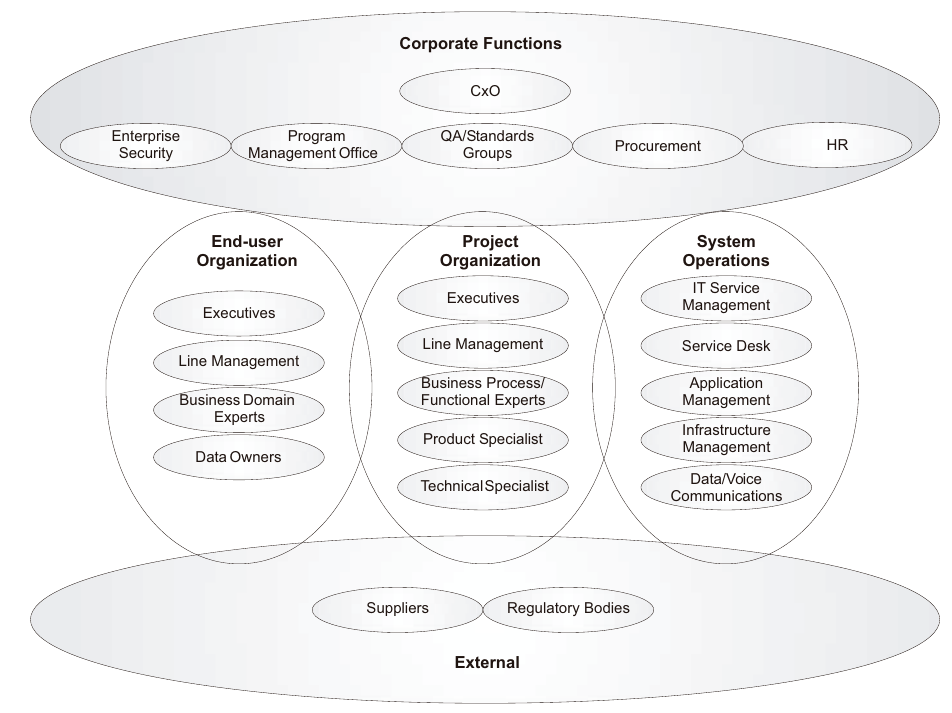
\includegraphics[width=\textwidth]{../figures/sample_stakeholders}
	\end{minipage}
	\hfill
	\begin{minipage}[bt]{0.496\textwidth}
		\centering
		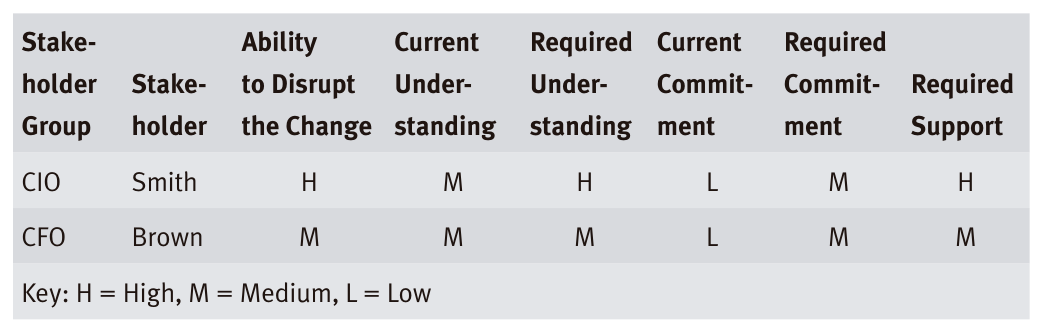
\includegraphics[width=\textwidth]{../figures/stakeholder_analysis}
		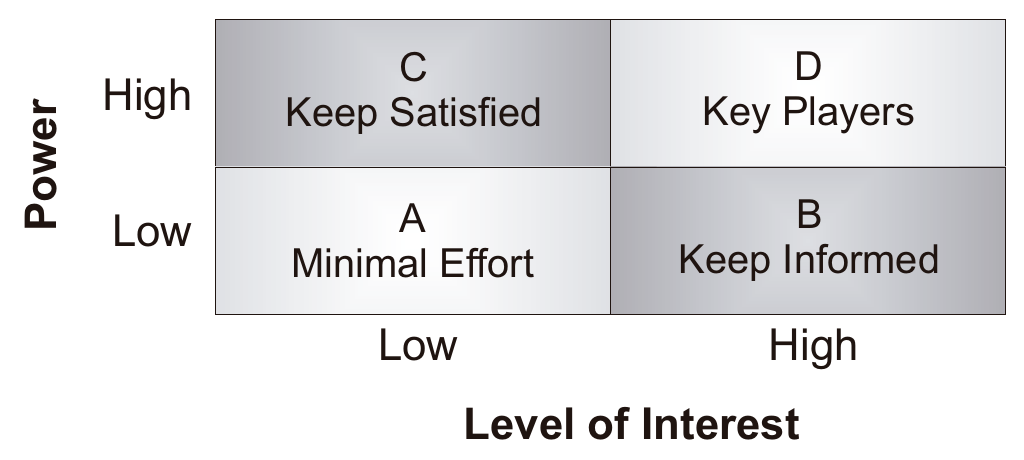
\includegraphics[width=\textwidth]{../figures/power_vs_interest}
	\end{minipage}
	\caption{Contoh Pemangku Kepentingan, Analisis Pemangku Kepentingan, Kekuatan vs Kepentingan}
	\label{fig:stakeholders}
\end{figure}

\subsection{Contoh Pemangku Kepentingan (Stakeholders)}
Dalam konteks transformasi menjadi hybrid working di Universitas ABC, pemangku kepentingan terbagi ke dalam beberapa kelompok, yang masing-masing memiliki peran dan tanggung jawab yang berbeda. Kelompok pemangku kepentingan tersebut meliputi:

\begin{itemize}
	\item \textbf{Corporate Functions:} 
	Fungsi korporat bertanggung jawab atas kebijakan dan strategi umum universitas. Contoh jabatan dalam kelompok ini meliputi Rektor, Wakil Rektor Bidang Akademik, dan Direktur Keuangan.
	
	\item \textbf{End-User Organization:} 
	Organisasi pengguna akhir terdiri dari mahasiswa dan dosen yang akan menggunakan sistem baru. Jabatan yang termasuk dalam kelompok ini antara lain Mahasiswa, Dosen, Pengajar dan Asisten Dosen.
	
	\item \textbf{Project Organization:} 
	Organisasi proyek terdiri dari tim yang terlibat dalam perencanaan dan pelaksanaan proyek transformasi. Jabatan yang ada dalam kelompok ini termasuk Manajer Proyek, Tim Arsitektur, Analis Bisnis, dan Tim Pengembangan TI.
	
	\item \textbf{System Operations:} 
	Tim operasi sistem bertanggung jawab untuk menjaga agar sistem berjalan dengan baik setelah implementasi. Jabatan dalam kelompok ini meliputi Administrator Sistem, Staf Dukungan TI, dan Teknisi Jaringan.
	
	\item \textbf{External:} 
	Pemangku kepentingan eksternal mencakup pihak-pihak yang berada di luar universitas tetapi berpengaruh terhadap proyek. Contoh jabatan dalam kelompok ini termasuk Vendor Teknologi, Konsultan Pendidikan, dan Badan Akreditasi.
\end{itemize}

\subsection{Analisis Kontribusi dan Kepentingan Posisi dalam Organisasi}

Dalam konteks transformasi hybrid working di universitas, analisis kontribusi dan kepentingan posisi dalam organisasi sangat penting untuk memastikan keberhasilan implementasi. Berikut adalah beberapa posisi kunci beserta analisisnya:

\begin{itemize}
	\item \textbf{Pimpinan Universitas (Rektor)}: 
	Memiliki kemampuan untuk mendisrupsi perubahan signifikan melalui pengambilan keputusan strategis dan penyediaan sumber daya. Pemahaman saat ini terhadap permasalahan dan solusi perlu dievaluasi, serta komitmen mereka untuk mendukung inisiatif hybrid working sangat penting.
	
	\item \textbf{Dekan Fakultas}: 
	Berperan sebagai penghubung antara kebijakan universitas dan kebutuhan program studi. Saat ini, mereka mungkin sudah memiliki pemahaman yang baik tentang permasalahan di tingkat fakultas. Namun, komitmen mereka untuk mendukung inisiatif ini perlu ditingkatkan agar dapat memberikan dukungan yang lebih besar kepada dosen dan mahasiswa.
	
	\item \textbf{Tim TI (Kepala IT)}: 
	Bertanggung jawab untuk mengeksekusi solusi teknis dan memastikan infrastruktur mendukung kebutuhan hybrid working. Tingkat dukungan yang mereka perlukan harus dinilai berdasarkan kemampuan mereka dalam menghadapi tantangan teknis. Peningkatan pemahaman mereka terhadap solusi yang akan diterapkan melalui pelatihan tambahan sangat diperlukan.
	
	\item \textbf{Mahasiswa}: 
	Sebagai pengguna akhir, pemahaman mereka tentang sistem baru yang akan mendukung pembelajaran hybrid perlu diperkuat. Tingkat dukungan yang diperlukan dari mereka dapat ditingkatkan melalui sosialisasi dan pelatihan mengenai teknologi baru, untuk memastikan adopsi dan komitmen terhadap perubahan.
\end{itemize}


\subsection{Penggunaan Kuadran Power dan Level of Interest}

Dalam analisis pemangku kepentingan untuk transformasi hybrid working di universitas, penggunaan kuadran kekuasaan (power) dan tingkat minat (interest) sangat penting untuk mengidentifikasi posisi-posisi kunci dan pendekatan yang tepat dalam melibatkan mereka. Kuadran ini dibagi menjadi empat kategori:

\begin{itemize}
	\item \textbf{Kuadran I: High Power, High Interest}
	\begin{itemize}
		\item \textbf{Contoh: Rektor}
		\item Rektor memiliki kekuasaan tinggi dalam pengambilan keputusan strategis dan juga sangat tertarik dengan keberhasilan transformasi hybrid working. Pendekatan yang tepat adalah memastikan komunikasi yang sering dan keterlibatan langsung dalam proses perencanaan dan implementasi.
	\end{itemize}
	
	\item \textbf{Kuadran II: High Power, Low Interest}
	\begin{itemize}
		\item \textbf{Contoh: Dewan Pengurus Universitas}
		\item Meskipun memiliki kekuasaan tinggi, mereka mungkin tidak memiliki ketertarikan yang mendalam terhadap detail operasional transformasi. Oleh karena itu, pendekatan yang efektif adalah memberikan informasi berkala yang relevan, serta memastikan bahwa keputusan strategis mereka sejalan dengan tujuan transformasi.
	\end{itemize}
	
	\item \textbf{Kuadran III: Low Power, High Interest}
	\begin{itemize}
		\item \textbf{Contoh: Mahasiswa}
		\item Mahasiswa mungkin tidak memiliki kekuasaan dalam pengambilan keputusan, tetapi mereka memiliki ketertarikan tinggi terhadap inisiatif yang mempengaruhi pengalaman belajar mereka. Untuk itu, penting untuk melibatkan mereka melalui forum diskusi, survei, dan pelatihan agar mereka merasa diikutsertakan dalam proses transformasi.
	\end{itemize}
	
	\item \textbf{Kuadran IV: Low Power, Low Interest}
	\begin{itemize}
		\item \textbf{Contoh: Staf Administrasi yang Tidak Terlibat Langsung}
		\item Posisi ini memiliki kekuasaan dan ketertarikan rendah terhadap proyek. Pendekatan yang diperlukan adalah minimal, hanya memberikan informasi yang diperlukan agar mereka tetap terinformasi tanpa membebani mereka dengan detail yang tidak relevan.
	\end{itemize}
\end{itemize}

Dengan memahami posisi masing-masing pemangku kepentingan dalam kuadran ini, universitas dapat mengembangkan strategi komunikasi dan keterlibatan yang lebih efektif untuk mendukung keberhasilan transformasi hybrid working.


\section{Peta Pemangku Kepentingan}
Lihat Gambar \ref{fig:stakeholders_map}.
\begin{figure}[h!]
	\centering
	\begin{minipage}[bt]{0.496\textwidth}
		\centering
		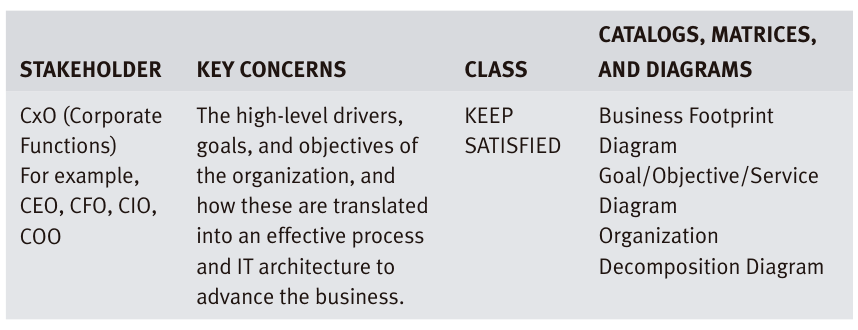
\includegraphics[width=\textwidth]{../figures/stakeholder_map_1}
		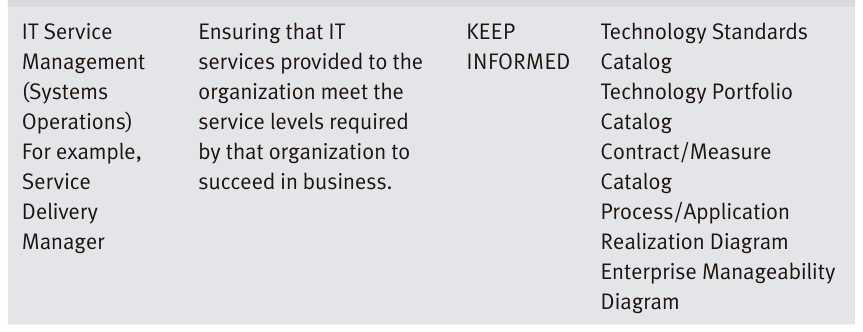
\includegraphics[width=\textwidth]{../figures/stakeholder_map_3}
	\end{minipage}
	\hfill
	\begin{minipage}[bt]{0.496\textwidth}
		\centering
		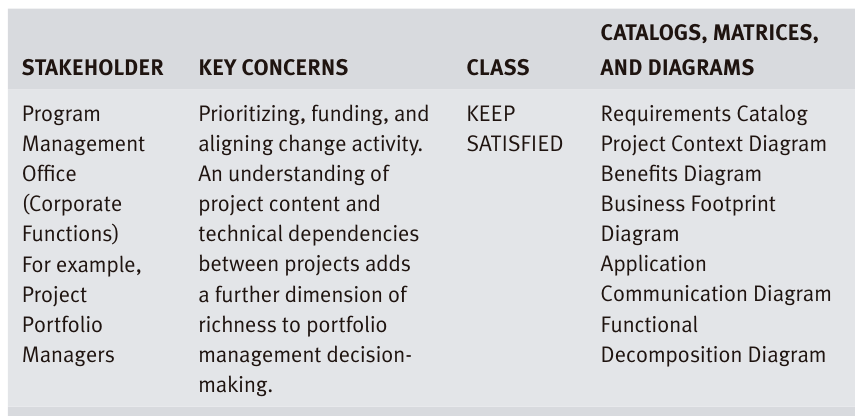
\includegraphics[width=\textwidth]{../figures/stakeholder_map_2}
	\end{minipage}
	\caption{Peta Pemangku Kepentingan}
	\label{fig:stakeholders_map}
\end{figure}


\subsection*{Contoh Keterkaitan antara Posisi Stakeholders dan Pola Komunikasi}

Keterkaitan antara posisi pemangku kepentingan dalam organisasi, keprihatinan utama mereka, dan pola komunikasi yang diterapkan adalah faktor penting dalam memastikan keberhasilan transformasi hybrid working di universitas. Berikut adalah analisis keterkaitan tersebut:

\begin{itemize}
	\item \textbf{Posisi Stakeholders dan Keprihatinan Utama}
	\begin{itemize}
		\item \textbf{Rektor (High Power, High Interest):} Rektor memiliki keprihatinan terhadap hasil akhir dari transformasi. Mereka fokus pada peningkatan pengalaman belajar mahasiswa dan efektivitas pengajaran.
		\item \textbf{Dekan Fakultas (High Power, Low Interest):} Dekan perlu memastikan bahwa kebijakan yang diterapkan sejalan dengan visi akademis, meskipun tidak terlibat dalam detail teknis. 
		\item \textbf{Mahasiswa (Low Power, High Interest):} Mahasiswa sangat peduli dengan aksesibilitas dan kualitas pembelajaran, yang langsung berdampak pada pengalaman belajar mereka.
		\item \textbf{Staf Administrasi (Low Power, Low Interest):} Mereka membutuhkan informasi yang cukup untuk mendukung kegiatan sehari-hari, namun tidak memerlukan keterlibatan mendalam.
	\end{itemize}
	
	\item \textbf{Pola Komunikasi}
	\begin{itemize}
		\item \textbf{Keep Satisfied:} Untuk pemangku kepentingan seperti Dewan Pengurus Universitas, penting untuk memberikan informasi strategis secara berkala, sehingga mereka merasa dilibatkan tanpa terlalu mendalami rincian proyek.
		\item \textbf{Key Players:} Rektor dan tim arsitektur harus berkomunikasi secara langsung dan rutin, menjaga mereka terinformasi tentang kemajuan dan tantangan dalam proyek.
		\item \textbf{Minimal Efforts:} Staf administrasi hanya perlu mendapatkan pembaruan dasar yang relevan untuk menjalankan tugas mereka tanpa detail tambahan.
		\item \textbf{Keep Informed:} Mahasiswa perlu mendapatkan informasi yang cukup mengenai perubahan yang akan mempengaruhi mereka, seperti pelatihan penggunaan platform baru dan cara berpartisipasi dalam feedback.
	\end{itemize}
	
	\item \textbf{Kaitannya dengan Alat-Alat Komunikasi di TOGAF}
	\begin{itemize}
		\item \textbf{Catalogs:} Penggunaan catalogs dapat membantu dalam menyusun daftar pemangku kepentingan, termasuk peran, keprihatinan utama, dan pola komunikasi yang diperlukan untuk masing-masing. Contoh: \textit{Stakeholder Catalog} yang merinci nama, jabatan, dan keprihatinan mereka.
		\item \textbf{Matrices:} Matriks keterkaitan antara pemangku kepentingan dan keprihatinan mereka dapat memberikan gambaran visual tentang siapa yang perlu dihubungi untuk isu tertentu. Contoh: \textit{Stakeholder Analysis Matrix} yang menghubungkan pemangku kepentingan dengan pola komunikasi dan jenis informasi yang dibutuhkan.
		\item \textbf{Diagrams:} Diagram alur dapat digunakan untuk menggambarkan pola komunikasi antar pemangku kepentingan, menunjukkan aliran informasi dan bagaimana setiap kelompok berinteraksi. Contoh: \textit{Communication Flow Diagram} yang menggambarkan interaksi antara rektor, dekan, dan mahasiswa dalam proses pengambilan keputusan.
	\end{itemize}
\end{itemize}

Dengan memahami keterkaitan posisi, keprihatinan, dan pola komunikasi yang sesuai, universitas dapat memastikan semua pemangku kepentingan terlibat secara efektif dalam proses transformasi hybrid working, menggunakan alat-alat komunikasi yang tepat untuk mendukung tujuan tersebut.


\section{Menilai Kesiapan untuk Transformasi}
\label{sec:kesiapan_transformasi}
\begin{itemize}
	\item Visi.
	\item Keinginan atau kesediaan untuk mencapai hasil.
	\item Persyaratan.
	\item Adanya indikasi/kasus dalam bisnis.
	\item Dana.
	\item Sponsorship dan kepemimpinan.
	\item Tata kelola.
	\item Akuntabilitas (kemampuan untuk dipertanggungjawabkan).
	\item Pendekatan dan model eksekusi yang dapat diterapkan.
	\item Kapasitas IT untuk mengeksekusi.
	\item Kapasitas perusahaan untuk mengeksekusi.
	\item Kemampuan perusahaan untuk mengimplementasikan dan mengoperasikan pasca eksekusi.
\end{itemize}

\subsection*{Contoh Menilai Kesiapan untuk Transformasi:}
\begin{itemize}
	\item \textbf{Visi.} Visi transformasi adalah untuk menciptakan pengalaman belajar hybrid yang terintegrasi, di mana mahasiswa dapat belajar secara fleksibel dan efisien, dengan dukungan teknologi yang memadai dan aksesibilitas yang tinggi.
	
	\item \textbf{Keinginan atau kesediaan untuk mencapai hasil.} Universitas ABC menunjukkan keinginan yang kuat untuk mencapai hasil yang diinginkan, yaitu peningkatan keterlibatan mahasiswa dan efektivitas pengajaran, dengan dukungan dari berbagai pemangku kepentingan.
	
	\item \textbf{Persyaratan (\textit{Requirements}).} Persyaratan untuk transformasi mencakup kebutuhan akan infrastruktur teknologi yang kuat, platform pembelajaran yang interaktif, dan pelatihan untuk dosen serta staf dalam penggunaan teknologi baru.
	
	\item \textbf{Adanya indikasi/kasus dalam bisnis.} Indikasi adanya kebutuhan untuk transformasi terlihat dari umpan balik mahasiswa yang menunjukkan ketidakpuasan terhadap pengalaman pembelajaran hybrid yang ada saat ini, serta meningkatnya permintaan untuk metode pembelajaran yang lebih fleksibel.
	
	\item \textbf{Dana.} Universitas telah mengalokasikan anggaran khusus untuk mendukung proyek transformasi ini, termasuk dana untuk pengembangan teknologi, pelatihan, dan peningkatan infrastruktur.
	
	\item \textbf{Sponsorship dan kepemimpinan.} Proyek ini didukung oleh pimpinan universitas, termasuk rektor dan dekan fakultas, yang berkomitmen untuk menyediakan sumber daya dan dukungan yang diperlukan untuk keberhasilan transformasi.
	
	\item \textbf{Tata kelola.} Proyek akan dikelola melalui komite pengawasan proyek yang terdiri dari perwakilan dari berbagai fakultas dan unit administrasi, memastikan bahwa semua aspek transformasi terkoordinasi dengan baik.
	
	\item \textbf{Akuntabilitas (kemampuan untuk dipertanggungjawabkan).} Setiap pemangku kepentingan akan memiliki peran dan tanggung jawab yang jelas dalam proyek, dengan mekanisme untuk menilai dan mempertanggungjawabkan kemajuan yang dicapai.
	
	\item \textbf{Pendekatan dan model eksekusi yang dapat diterapkan.} Pendekatan agile akan digunakan untuk memastikan bahwa transformasi dapat beradaptasi dengan kebutuhan yang berubah dan memberikan hasil yang cepat serta iteratif.
	
	\item \textbf{Kapasitas IT untuk mengeksekusi.} Tim TI universitas memiliki keterampilan dan pengalaman yang diperlukan untuk mendukung pengembangan dan implementasi sistem teknologi yang diperlukan untuk transformasi.
	
	\item \textbf{Kapasitas perusahaan untuk mengeksekusi.} Universitas memiliki kapasitas yang cukup dalam hal sumber daya manusia dan infrastruktur untuk melaksanakan transformasi ini, dengan adanya dukungan dari berbagai fakultas dan unit.
	
	\item \textbf{Kemampuan perusahaan untuk mengimplementasikan dan mengoperasikan pasca eksekusi.} Setelah implementasi, universitas akan membentuk tim dukungan untuk memastikan bahwa semua sistem dan proses baru dapat beroperasi dengan lancar, serta memberikan pelatihan berkelanjutan kepada dosen dan staf.
\end{itemize}


\section{Visi Arsitektur}
\label{sec:visi_arsitektur}
\begin{itemize}
	\item Deskripsi masalah, termasuk pemangku kepentingan dan kekhawatiran mereka, serta daftar masalah/skenario yang perlu diatasi.
	\item Tujuan dari \textit{Architectural Work Statement}.
	\item Ringkasan pandangan yang diperlukan untuk Arsitektur tingkat tinggi dan Permintaan Pekerjaan Arsitektur Bisnis, Aplikasi, Data, dan Teknologi.
	\item Skenario bisnis.
	\item Kebutuhan pemangku kepentingan yang telah dipetakan dan dirinci.
\end{itemize}

\subsection*{Contoh Visi Arsitektur:}
\begin{itemize}
	\item \textbf{Deskripsi masalah}. Universitas ABC menghadapi tantangan dalam memberikan pengalaman belajar yang terintegrasi antara mode pembelajaran fisik dan daring. Pemangku kepentingan yang terlibat, termasuk mahasiswa, dosen, dan staf administrasi, memiliki kekhawatiran terkait aksesibilitas materi pembelajaran, keterlibatan mahasiswa dalam kelas hybrid, dan efisiensi penggunaan teknologi. Masalah yang perlu diatasi mencakup:
	\begin{itemize}
		\item Kurangnya aksesibilitas teknologi untuk mahasiswa yang belajar dari rumah.
		\item Kesulitan dalam kolaborasi antara mahasiswa yang hadir secara fisik dan yang berpartisipasi secara daring.
		\item Ketidakpuasan mahasiswa terhadap pengalaman belajar hybrid.
	\end{itemize}
	
	\item \textbf{Tujuan dari \textit{Architectural Work Statement}}. Tujuan dari dokumen ini adalah untuk merumuskan strategi arsitektur yang mendukung implementasi pembelajaran hybrid di Universitas ABC, memastikan bahwa semua pemangku kepentingan memiliki akses yang setara terhadap materi pembelajaran dan dapat berpartisipasi dalam interaksi akademik secara efektif.
	
	\item \textbf{Ringkasan pandangan}. Visi arsitektur tingkat tinggi mencakup integrasi sistem informasi akademik dengan platform kolaborasi untuk menciptakan lingkungan belajar yang seamless. Permintaan pekerjaan arsitektur mencakup pengembangan solusi di area Bisnis, Aplikasi, Data, dan Teknologi, dengan fokus pada:
	\begin{itemize}
		\item \textbf{Bisnis:} Meningkatkan pengalaman belajar mahasiswa dan keterlibatan dosen dalam kelas hybrid.
		\item \textbf{Aplikasi:} Pengembangan aplikasi pembelajaran yang mendukung interaksi real-time.
		\item \textbf{Data:} Penyediaan data analitik untuk melacak keterlibatan dan kinerja mahasiswa.
		\item \textbf{Teknologi:} Penyediaan infrastruktur teknologi yang handal untuk mendukung pembelajaran hybrid.
	\end{itemize}
	
	\item \textbf{Skenario bisnis}. Proyek ini bertujuan untuk memperkuat keterhubungan antara mahasiswa yang belajar secara daring dan luring, mengoptimalkan penggunaan ruang kelas dengan teknologi terbaru, dan menciptakan metode pembelajaran yang adaptif untuk memenuhi kebutuhan mahasiswa dari berbagai latar belakang.
	
	\item \textbf{Kebutuhan pemangku kepentingan yang telah dipetakan dan dirinci}. Kebutuhan pemangku kepentingan mencakup:
	\begin{itemize}
		\item \textbf{Mahasiswa:} Akses mudah ke materi pembelajaran dan dukungan teknis yang memadai.
		\item \textbf{Dosen:} Alat yang memungkinkan pengajaran efektif di kelas hybrid dan dukungan dalam mengevaluasi kinerja mahasiswa.
		\item \textbf{Staf Administrasi:} Sistem untuk memantau keterlibatan mahasiswa dan efektivitas program hybrid.
	\end{itemize}
	Setiap kebutuhan akan dipetakan ke dalam rencana implementasi untuk memastikan bahwa solusi arsitektur memenuhi harapan semua pemangku kepentingan.
\end{itemize}

\section{Skenario Bisnis}
\label{sec:skenario_bisnis}
\begin{itemize}
	\item \textbf{Masalah}. Mengidentifikasi, mendokumentasikan, dan memberi peringkat pada masalah yang menjadi pendorong proyek.
	\item \textbf{Lingkungan Bisnis dan Teknis}. Mendokumentasikan sebagai model arsitektur tingkat tinggi lingkungan bisnis dan teknis di mana situasi masalah terjadi.
	\item \textbf{Tujuan dan Ukuran Keberhasilan}. Mengidentifikasi dan mendokumentasikan tujuan yang diharapkan, hasil dari penyelesaian masalah yang berhasil.
	\item \textbf{Aktor Manusia}. Mengidentifikasi aktor manusia dan peran mereka dalam model bisnis, partisipan manusia, dan perannya.
	\item \textbf{Aktor Komputer}. Mengidentifikasi aktor komputer dan peran mereka dalam model teknologi, elemen komputasi, dan perannya.
	\item \textbf{Peran dan Tanggung Jawab}. Mengidentifikasi dan mendokumentasikan peran, tanggung jawab, dan ukuran keberhasilan setiap aktor, skrip yang dibutuhkan setiap aktor, dan hasil yang diharapkan dari penanganan situasi yang tepat.
	\item \textbf{Revisi}. Memeriksa kesesuaian tujuan untuk menginspirasi pekerjaan arsitektur selanjutnya, dan menyempurnakan hanya jika diperlukan.
\end{itemize}

\subsection*{Contoh Skenario Bisnis:}
\begin{itemize}
	\item \textbf{Masalah}. Universitas ABC menghadapi tantangan dalam menyediakan pengalaman belajar yang seimbang antara interaksi fisik dan digital, dengan meningkatnya jumlah mahasiswa yang memilih model pembelajaran hybrid. Masalah ini mencakup kurangnya infrastruktur teknologi yang mendukung, kesulitan dalam kolaborasi antara mahasiswa, dan perbedaan dalam aksesibilitas materi pembelajaran.
	
	\item \textbf{Lingkungan Bisnis dan Teknis}. Lingkungan bisnis mencakup semua fakultas di Universitas ABC, yang melayani mahasiswa dari berbagai latar belakang. Lingkungan teknis melibatkan platform pembelajaran daring (misalnya, Learning Management System), alat kolaborasi (seperti Microsoft Teams), serta perangkat keras di ruang kelas seperti proyektor dan sistem audio untuk mendukung interaksi daring dan luring.
	
	\item \textbf{Tujuan dan Ukuran Keberhasilan}. Tujuan dari proyek ini adalah meningkatkan pengalaman belajar mahasiswa dengan menyediakan platform yang memungkinkan kolaborasi efektif antara mahasiswa yang hadir secara fisik dan daring. Ukuran keberhasilan dapat diukur melalui survei kepuasan mahasiswa, peningkatan partisipasi dalam kelas, dan evaluasi hasil akademik yang menunjukkan peningkatan minimal 15\% dalam nilai akhir mahasiswa.
	
	\item \textbf{Aktor Manusia}. Aktor manusia yang terlibat dalam model bisnis ini mencakup:
	\begin{itemize}
		\item \textbf{Mahasiswa:} Menghadiri kelas baik secara daring maupun luring dan berkolaborasi dalam proyek.
		\item \textbf{Dosen:} Mengajar dan memfasilitasi interaksi antara mahasiswa di kelas fisik dan virtual.
		\item \textbf{Staf TI:} Menyediakan dukungan teknis dan pemeliharaan sistem teknologi yang digunakan.
	\end{itemize}
	
	\item \textbf{Aktor Komputer}. Aktor komputer dalam model teknologi mencakup:
	\begin{itemize}
		\item \textbf{Platform Pembelajaran Daring:} Sistem yang digunakan untuk menyampaikan materi pembelajaran dan memfasilitasi interaksi.
		\item \textbf{Alat Kolaborasi:} Alat yang digunakan untuk komunikasi dan kolaborasi, seperti Microsoft Teams dan Google Meet.
		\item \textbf{Sistem Manajemen Data:} Database yang menyimpan informasi tentang mahasiswa, dosen, dan materi pembelajaran.
	\end{itemize}
	
	\item \textbf{Peran dan Tanggung Jawab}. Peran dan tanggung jawab setiap aktor mencakup:
	\begin{itemize}
		\item \textbf{Mahasiswa:} Berpartisipasi aktif dalam kelas, memberikan umpan balik mengenai pengalaman belajar.
		\item \textbf{Dosen:} Menyusun materi pembelajaran yang sesuai untuk format hybrid dan mengevaluasi partisipasi serta kinerja mahasiswa.
		\item \textbf{Staf TI:} Memastikan semua alat dan platform berjalan dengan baik, memberikan pelatihan teknis kepada dosen dan mahasiswa.
	\end{itemize}
	Ukuran keberhasilan setiap aktor dapat diukur melalui kinerja individu dan umpan balik dari pemangku kepentingan lainnya.
	
	\item \textbf{Revisi}. Revisi dilakukan secara berkala berdasarkan umpan balik dari mahasiswa dan dosen untuk memastikan bahwa tujuan proyek tetap relevan dan inspiratif untuk pengembangan arsitektur lebih lanjut. Jika diperlukan, langkah-langkah dapat disempurnakan untuk meningkatkan efektivitas pelaksanaan pembelajaran hybrid.
\end{itemize}


\section{Dokumen \textit{Architectural Statement of Work}}
\label{sec:stament_of_work}
\begin{itemize}
	\item Judul.
	\item Permintaan Proyek Arsitektur dan Latar Belakang.
	\item Deskripsi Proyek Arsitektur dan Ruang Lingkup.
	\item Ikhtisar Visi Arsitektur.
	\item Prosedur Khusus Perubahan Ruang Lingkup.
	\item Peran, Tanggung Jawab, dan Deliverables.
	\item Kriteria dan Prosedur Penerimaan.
	\item Rencana dan Jadwal Proyek Arsitektur.
	\item Persetujuan.
\end{itemize}

\subsection*{Contoh Dokumen:}
\begin{itemize}
	\item \textbf{Judul.} 
	Architectural Statement of Work untuk Implementasi Hybrid Working di Universitas ABC.
	
	\item \textbf{Permintaan Proyek Arsitektur dan Latar Belakang.} 
	Permintaan untuk proyek arsitektur ini muncul dari kebutuhan Universitas ABC untuk menyediakan lingkungan belajar yang fleksibel dan mendukung pembelajaran hybrid sebagai respon terhadap perubahan dalam cara mahasiswa belajar yang terjadi akibat pandemi COVID-19 dan perkembangan teknologi pendidikan.
	
	\item \textbf{Deskripsi Proyek Arsitektur dan Ruang Lingkup.} 
	Proyek ini bertujuan untuk merancang dan mengimplementasikan sistem yang mendukung pembelajaran hybrid, mencakup pengembangan platform kolaborasi seperti Microsoft Teams dan Zoom, integrasi sistem informasi akademik seperti SIAKAD, serta perancangan ulang ruang kelas untuk mendukung interaksi daring dan luring dengan menggunakan teknologi proyeksi dan alat interaksi digital.
	
	\item \textbf{Ikhtisar Visi Arsitektur.} 
	Visi arsitektur adalah menciptakan pengalaman belajar yang seamless antara interaksi fisik dan digital, memungkinkan mahasiswa untuk mengakses materi pembelajaran secara daring, berkolaborasi dengan sesama mahasiswa dalam proyek kelompok, dan berinteraksi dengan dosen melalui sesi tatap muka dan daring secara fleksibel.
	
	\item \textbf{Prosedur Khusus Perubahan Ruang Lingkup.} 
	Prosedur untuk perubahan ruang lingkup meliputi pengajuan permintaan tertulis oleh pemangku kepentingan seperti dosen dan mahasiswa, evaluasi dampak perubahan oleh tim arsitektur, serta persetujuan perubahan oleh komite pengawasan proyek yang terdiri dari perwakilan fakultas dan IT.
	
	\item \textbf{Peran, Tanggung Jawab, dan Deliverables.} 
	Peran dalam proyek ini mencakup:
	\begin{itemize}
		\item \textbf{Manajer Proyek:} Bertanggung jawab untuk pengelolaan keseluruhan proyek dan komunikasi dengan pemangku kepentingan.
		\item \textbf{Tim Arsitektur:} Bertanggung jawab untuk perancangan solusi teknis dan strategi implementasi.
		\item \textbf{Staf TI:} Bertanggung jawab untuk implementasi teknis, pemeliharaan, dan dukungan sistem.
	\end{itemize}
	Deliverables mencakup dokumen perancangan yang detail, prototipe sistem, dan laporan kemajuan proyek yang disampaikan setiap bulan.
	
	\item \textbf{Kriteria dan Prosedur Penerimaan.} 
	Kriteria penerimaan mencakup penyelesaian proyek sesuai dengan spesifikasi yang disepakati, serta hasil evaluasi pengguna yang menunjukkan tingkat kepuasan yang tinggi (minimal 80\%). Prosedur penerimaan melibatkan pengujian fungsional dan evaluasi oleh pemangku kepentingan setelah fase implementasi.
	
	\item \textbf{Rencana dan Jadwal Proyek Arsitektur.} 
	Rencana proyek mencakup fase-fase utama seperti perencanaan (2 bulan), desain (1 bulan), implementasi (3 bulan), dan evaluasi (1 bulan). Jadwal proyek akan dibagi menjadi beberapa milestone, dengan estimasi waktu untuk masing-masing fase, di mana setiap fase akan dievaluasi pada akhir periode masing-masing.
	
	\item \textbf{Persetujuan.} 
	Dokumen ini memerlukan persetujuan dari pemangku kepentingan utama, termasuk Rektor Universitas ABC, Dekan Fakultas Ilmu Komputer, dan perwakilan mahasiswa, sebelum proyek dapat dilanjutkan ke fase berikutnya.
\end{itemize}


\section{Ringkasan}
\begin{itemize}
	\item Fase \textit{Architectural Vision} adalah langkah pertama dalam Metode Pengembangan Arsitektur TOGAF, di mana ruang lingkup didefinisikan, pemangku kepentingan diidentifikasi, dan visi arsitektur tingkat tinggi ditetapkan.
	\item Fase ini penting untuk memastikan bahwa proyek arsitektur memiliki dukungan dan arahan yang tepat sejak awal.
\end{itemize}

\section{Kegiatan Kelas dan Tugas}
Buatlah visi untuk kapabilitas arsitektur yang Anda pilih, berdasarkan informasi yang dikumpulkan dalam fase Preliminary dan fase ini. Deskripsikan keadaan saat ini (As-Is) dan keadaan target (To-Be) untuk memperjelas visi arsitektur tersebut dalam bentuk kajian kesiapan (Subbab \ref{sec:kesiapan_transformasi}), kajian \textit{stakeholders} (Subbab \ref{sec:stakholders}), perumusan visi arsitektur (Subbab \ref{sec:visi_arsitektur}), kajian skenario bisnis (Subbab \ref{sec:skenario_bisnis}), dan dokumen \textit{Architectural Statement of Work}(Subbab \ref{sec:stament_of_work}).

	\chapter{Arsitektur Bisnis}

\section{Tujuan}
Tujuan utama dari Pengembangan Arsitektur Bisnis adalah sebagai berikut:
\begin{enumerate}
	\item Membangun Arsitektur Bisnis Target yang menjelaskan bagaimana perusahaan seharusnya beroperasi untuk mencapai tujuan bisnis, serta menanggapi pendorong strategis bisnis (\textit{business strategic drivers}) yang telah ditetapkan dalam Visi Arsitektur. Target arsitektur yang harus memenuhi atau menjawab \textit{Permintaan Pekerjaan Arsitektur} dan menjawab kekhawatiran para pemangku kepentingan (\textit{stakeholders}).
	\item Mengidentifikasi komponen dari Peta Jalan Arsitektur (\textit{architecture roadmap}) berdasarkan kesenjangan (\textit{gap}) antara Arsitektur Saat Ini dan Arsitektur Bisnis Target.
\end{enumerate}

\section{Input}
Input yang penting untuk Pengembangan Arsitektur Bisnis adalah sebagai berikut. Pada umumnya output dari fase-fase sebelumnya menjadi input pada fase ini. Pembahasan setiap item input pada fase ini bisa dilhat pada pembahasan mereka di fase-fase (bab-bab) sebelumnya.
\begin{enumerate}
	\item Prinsip bisnis, tujuan bisnis, dan pendorong bisnis
	\item Penilaian Kapabilitas
	\item Rencana Komunikasi
	\item Model Organisasi untuk Arsitektur Perusahaan
	\item Kerangka Arsitektur yang Disesuaikan
	\item Pernyataan Pekerjaan Arsitektur yang telah disetujui
	\item Prinsip Arsitektur, termasuk prinsip bisnis yang telah ada sebelumnya
	\item Company Continuum
	\item Repositori Arsitektur
	\item Visi Arsitektur, termasuk:
	\begin{itemize}
		\item Masalah
		\item Tujuan Pernyataan Pekerjaan Arsitektur
		\item Ringkasan gambaran umum
		\item Skenario bisnis (opsional)
		\item Persyaratan pemangku kepentingan tingkat tinggi secara rinci
	\end{itemize}
	\item Draf Dokumen Definisi Arsitektur, termasuk (jika dalam cakupan):
	\begin{itemize}
		\item Arsitektur Bisnis Dasar (tingkat tinggi)
		\item Arsitektur Data Dasar (tingkat tinggi)
		\item Arsitektur Aplikasi Dasar (tingkat tinggi)
		\item Arsitektur Teknologi Dasar (tingkat tinggi)
		\item Arsitektur Bisnis Target (tingkat tinggi)
		\item Arsitektur Data Target (tingkat tinggi)
		\item Arsitektur Aplikasi Target (tingkat tinggi)
		\item Arsitektur Teknologi Target (tingkat tinggi)
	\end{itemize}
	\item Permintaan untuk Pekerjaan Arsitektur
\end{enumerate}

\section{Langkah-Langkah}
Langkah-langkah dalam Pengembangan Arsitektur Bisnis adalah sebagai berikut:
\begin{enumerate}
	\item Memilih model referensi, sudut pandang dari berbagai aktor, dan alat
	\item Mengembangkan Deskripsi Arsitektur Bisnis Saat Ini
	\item Mengembangkan Deskripsi Arsitektur Bisnis Target
	\item Melakukan Analisis Kesenjangan
	\item Menentukan komponen dari peta jalan
	\item Membuat solusi untuk dampak atau efek samping di seluruh Lanskap Arsitektur
	\item Melakukan tinjauan formal pemangku kepentingan terhadap arsitektur yang diusulkan
	\item Menyelesaikan Arsitektur Bisnis
	\item Membuat Dokumen Definisi Arsitektur
\end{enumerate}

\subsection*{Contoh:}
Berikut adalah contoh penerapan langkah-langkah pengembangan arsitektur bisnis dalam konteks Hybrid Teaching and Learning di universitas:

\begin{enumerate}
	\item \textbf{Memilih model referensi, sudut pandang dari berbagai aktor, dan alat:}  
	Dalam konteks Hybrid Teaching and Learning, model referensi yang dipilih dapat berupa model pendidikan campuran (blended learning) yang menggabungkan pembelajaran daring dan luring. Sudut pandang yang dipertimbangkan termasuk dari sisi mahasiswa, dosen, staf IT, serta administrasi universitas. Alat yang dipilih mencakup platform LMS (Learning Management System) seperti Moodle, Zoom untuk pembelajaran daring, dan infrastruktur fisik kampus untuk pembelajaran luring.
	
	\item \textbf{Mengembangkan Deskripsi Arsitektur Bisnis Saat Ini:}  
	Deskripsi arsitektur saat ini mungkin mencakup penggunaan pembelajaran tatap muka secara dominan sebelum pandemi, dengan sistem pendukung minimal untuk pembelajaran daring. Infrastruktur teknologi yang ada mungkin terbatas pada penggunaan email dan forum diskusi.
	
	\item \textbf{Mengembangkan Deskripsi Arsitektur Bisnis Target:}  
	Arsitektur target dapat menggambarkan integrasi penuh antara pembelajaran daring dan luring, dengan platform digital yang kuat untuk manajemen konten, interaksi kelas, penilaian, dan pelaporan. Sistem harus mendukung fleksibilitas bagi mahasiswa untuk memilih mode belajar yang sesuai, baik dari rumah maupun kampus.
	
	\item \textbf{Melakukan Analisis Kesenjangan:}  
	Analisis kesenjangan dilakukan dengan membandingkan infrastruktur dan proses pembelajaran saat ini dengan target hybrid. Misalnya, kesenjangan dapat ditemukan pada kurangnya platform pembelajaran yang mudah diakses, kurangnya pelatihan bagi dosen untuk mengajar secara efektif secara daring, dan kebutuhan akan peningkatan infrastruktur jaringan di kampus.
	
	\item \textbf{Menentukan Komponen dari Peta Jalan:}  
	Komponen dari peta jalan untuk mengimplementasikan Hybrid Teaching and Learning mungkin mencakup pelatihan dosen tentang platform daring, peningkatan kapasitas server untuk mendukung akses mahasiswa, serta pengembangan kebijakan fleksibel mengenai kehadiran dan penilaian.
	
	\item \textbf{Membuat Solusi untuk Dampak atau Efek Samping di Seluruh Lanskap Arsitektur:}  
	Solusi untuk dampak potensial mungkin termasuk memastikan bahwa ada dukungan teknis yang memadai untuk mahasiswa dan dosen dalam menggunakan platform daring, mengatasi potensi kesenjangan akses teknologi di antara mahasiswa, dan memitigasi kekhawatiran mengenai interaksi sosial yang terbatas pada pembelajaran daring.
	
	\item \textbf{Melakukan Tinjauan Formal Pemangku Kepentingan terhadap Arsitektur yang Diusulkan:}  
	Tinjauan dilakukan oleh dekan, kepala departemen, dosen, mahasiswa, dan staf IT untuk memastikan bahwa solusi hybrid yang diusulkan memenuhi kebutuhan dan kemampuan seluruh pemangku kepentingan, baik dari segi teknologi, akademik, maupun administratif.
	
	\item \textbf{Menyelesaikan Arsitektur Bisnis:}  
	Setelah tinjauan pemangku kepentingan, rencana arsitektur final diselesaikan dengan penyesuaian sesuai umpan balik yang diberikan. Solusi hybrid final melibatkan sistem yang terintegrasi dengan baik antara pembelajaran daring dan luring, memastikan kemudahan transisi di antara keduanya.
	
	\item \textbf{Membuat Dokumen Definisi Arsitektur:}  
	Dokumen ini akan mencakup deskripsi detail tentang arsitektur hybrid yang diusulkan, termasuk platform teknologi yang digunakan, prosedur operasional, kebijakan pembelajaran, serta peta jalan implementasi secara menyeluruh.
\end{enumerate}

\section{Output}
Output yang diharapkan dari fase ini meliputi:
\begin{enumerate}
	\item Pernyataan Pekerjaan Arsitektur yang diperbarui sesuai kebutuhan
	\item Prinsip bisnis, tujuan bisnis, dan pendorong bisnis yang divalidasi
	\item Prinsip Arsitektur Bisnis yang diperbarui
	\item Draf Dokumen Definisi Arsitektur, termasuk konten yang diperbarui
	\item Draf Spesifikasi Persyaratan Arsitektur, termasuk konten yang diperbarui
	\item Komponen Arsitektur Bisnis dari Peta Jalan Arsitektur
\end{enumerate}

\subsection*{Contoh:}
Berikut adalah contoh penerapan elemen-elemen keluaran arsitektur bisnis dalam konteks Hybrid Teaching and Learning di universitas:

\begin{enumerate}
	\item \textbf{Pernyataan Pekerjaan Arsitektur yang diperbarui sesuai kebutuhan:}  
	Dalam konteks Hybrid Teaching and Learning, pernyataan pekerjaan arsitektur dapat diperbarui untuk mencerminkan perubahan dalam strategi pembelajaran yang melibatkan metode daring dan luring. Ini termasuk penambahan spesifikasi teknis untuk platform e-learning yang digunakan serta prosedur untuk dukungan teknologi dan pengembangan kurikulum berbasis hybrid.
	
	\item \textbf{Prinsip bisnis, tujuan bisnis, dan pendorong bisnis yang divalidasi:}  
	Prinsip-prinsip dan tujuan yang divalidasi untuk universitas dalam sistem hybrid dapat mencakup fleksibilitas dalam metode pengajaran, peningkatan aksesibilitas pembelajaran bagi mahasiswa dari berbagai lokasi, serta pengurangan hambatan fisik dalam proses pembelajaran. Pendorong bisnis mungkin meliputi efisiensi operasional dan peningkatan daya tarik bagi mahasiswa internasional.
	
	\item \textbf{Prinsip Arsitektur Bisnis yang diperbarui:}  
	Prinsip-prinsip arsitektur bisnis dapat diperbarui (ditambahkan, dihapus, dsb.) untuk memastikan bahwa teknologi digital dan infrastruktur fisik universitas mendukung metode pembelajaran hybrid. Contoh, misalnya penambahan prinsip-prinsip: fokus pada interoperabilitas platform teknologi, kelancaran transisi antara mode daring dan luring, serta kesesuaian dengan tujuan institusi.
	
	\item \textbf{Draf Dokumen Definisi Arsitektur, termasuk konten yang diperbarui:}  
	Dalam draf dokumen ini, arsitektur hybrid akan dijabarkan, mencakup komponen-komponen teknologi seperti Learning Management System (LMS), sistem komunikasi daring (misalnya Zoom atau Microsoft Teams), serta infrastruktur fisik kampus yang siap mendukung pembelajaran tatap muka dan daring secara bersamaan.
	
	\item \textbf{Draf Spesifikasi Persyaratan Arsitektur, termasuk konten yang diperbarui:}  
	Spesifikasi persyaratan arsitektur akan diperbarui untuk mencerminkan kebutuhan teknologi dan operasional yang lebih rinci, seperti persyaratan bandwidth internet, kebutuhan perangkat keras di ruang kelas, dan standar keamanan data yang digunakan dalam sistem pembelajaran daring.
	
	\item \textbf{Komponen Arsitektur Bisnis dari Peta Jalan Arsitektur:}  
	Komponen arsitektur bisnis untuk peta jalan akan mencakup pengembangan bertahap infrastruktur teknologi, pelatihan staf dan dosen untuk mengoperasikan sistem hybrid, serta penjadwalan transisi dari sistem pembelajaran tatap muka tradisional menuju metode hybrid yang lebih adaptif.
\end{enumerate}

\section{Menggunakan Repositori Arsitektur dan \textit{Enterprise Continuum}}
Tim arsitektur perlu mempertimbangkan sumber daya Arsitektur Bisnis yang relevan dari Repositori Arsitektur atau dari \textit{Enterprise Continuum} (solusi dan standar dari umum sampai spesifik), terutama:
\begin{enumerate}
	\item Standar umum yang berlaku (standard internasional dan nasional)
	\item Model bisnis umum yang relevan dengan sektor industri organisasi (industri pendidikan)
	\item Model bisnis yang relevan dengan domain bisnis (industri pendidikan tinggi)
	\item Blok bangunan spesifik perusahaan (spesifik terhadap universitas tersebut)
\end{enumerate}

\subsection{Contoh:}
Dalam penerapan Hybrid Teaching and Learning di universitas, tim arsitektur perlu mempertimbangkan sumber daya Arsitektur Bisnis yang relevan dari Repositori Arsitektur atau dari \textit{Enterprise Continuum}. Berikut adalah contoh penerapannya:

\begin{enumerate}
	\item \textbf{Standar umum yang berlaku:}  
	Standar internasional dan nasional yang relevan mencakup standar teknologi pembelajaran seperti ISO/IEC 40180 untuk sistem e-learning, dan standar aksesibilitas web (seperti WCAG 2.1) yang memastikan bahwa platform daring dapat diakses oleh semua mahasiswa, termasuk mereka yang memiliki keterbatasan fisik. Di tingkat nasional, pedoman dari Kementerian Pendidikan terkait pembelajaran digital juga harus dipatuhi.
	
	\item \textbf{Model bisnis umum yang relevan dengan sektor industri pendidikan:}  
	Model bisnis dalam sektor industri pendidikan mencakup penyediaan layanan pendidikan berkualitas yang dapat diakses secara daring dan luring, dengan fokus pada peningkatan pengalaman belajar mahasiswa melalui teknologi. Contoh penerapannya adalah integrasi LMS (Learning Management System) dengan sistem administrasi akademik yang memudahkan manajemen pembelajaran dan administrasi universitas.
	
	\item \textbf{Model bisnis yang relevan dengan domain bisnis pendidikan tinggi:}  
	Dalam konteks pendidikan tinggi, model bisnis hybrid teaching melibatkan penyusunan program kuliah yang fleksibel, penyediaan kuliah daring bagi mahasiswa yang tidak dapat hadir di kampus, dan integrasi evaluasi pembelajaran secara digital. Selain itu, kolaborasi antara dosen dan mahasiswa dapat diperluas dengan penggunaan platform digital untuk seminar atau kuliah tamu dari pakar luar negeri.
	
	\item \textbf{Blok bangunan spesifik universitas:}  
	Blok bangunan spesifik universitas meliputi infrastruktur teknologi seperti ruang kelas pintar yang dilengkapi perangkat audio-visual, jaringan internet berkecepatan tinggi, platform LMS khusus yang disesuaikan dengan kebutuhan universitas, serta kebijakan internal yang mengatur penggunaan teknologi dalam pembelajaran hybrid. Selain itu, termasuk pengembangan modul pelatihan bagi dosen untuk mengoptimalkan pembelajaran daring.
\end{enumerate}


\section{Identifikasi Katalog, Matriks, dan Diagram}
\begin{enumerate}
	\item Katalog mengumpulkan inventaris aset inti bisnis.
	\item Matriks menunjukkan hubungan antara entitas model.
	\item Diagram menggambarkan informasi Arsitektur Bisnis dari berbagai perspektif (sudut pandang).
\end{enumerate}

\subsection{Contoh:}
Dalam konteks Hybrid Teaching and Learning di universitas, identifikasi Katalog, Matriks, dan Diagram dapat diterapkan sebagai berikut:

\begin{enumerate}
	\item \textbf{Katalog:}  
	Katalog mengumpulkan inventaris aset inti yang digunakan dalam pembelajaran hybrid. Contoh aset inti di universitas meliputi:
	\begin{itemize}
		\item \textbf{Katalog Sumber Daya Digital:} Buku elektronik, jurnal akademik daring, video pembelajaran, dan modul interaktif yang tersedia dalam platform LMS.
		\item \textbf{Katalog Perangkat Keras:} Laptop, tablet, proyektor, dan peralatan audio-visual yang digunakan dalam pengajaran luring maupun daring.
		\item \textbf{Katalog Kursus:} Daftar semua kursus yang ditawarkan secara hybrid, termasuk deskripsi, jadwal, dan metodologi pengajaran.
		\item \textbf{Katalog Dosen:} Informasi mengenai dosen yang mengajar di program hybrid, termasuk kualifikasi, pengalaman, dan area keahlian.
		\item \textbf{Katalog Alat dan Aplikasi:} Daftar aplikasi dan alat yang digunakan dalam pembelajaran, seperti platform komunikasi (Zoom, Microsoft Teams), alat kolaborasi (Google Workspace), dan perangkat lunak pengelolaan kelas.
	\end{itemize}
	
	\item \textbf{Matriks:}  
	Matriks menunjukkan hubungan antara berbagai entitas dalam model pembelajaran hybrid. Contoh dalam konteks universitas adalah:
	\begin{itemize}
		\item \textbf{Matriks Keterkaitan Kursus dan Dosen:} Matriks ini menunjukkan hubungan antara dosen yang mengajar dan kursus yang ditawarkan. Misalnya, kolom mencantumkan nama dosen, sedangkan baris mencantumkan nama kursus. Sel-sel di dalam matriks dapat diisi dengan tanda centang atau nilai yang menunjukkan apakah seorang dosen mengajar kursus tertentu.
		
		\item \textbf{Matriks Keterlibatan Mahasiswa:} Matriks yang menunjukkan keterlibatan mahasiswa dalam pembelajaran daring versus luring. Kolom dapat mencakup nama mahasiswa, sedangkan baris mencakup aktivitas pembelajaran seperti mengikuti kuliah luring, menghadiri sesi diskusi daring, atau mengerjakan tugas daring. Sel-sel dapat diisi dengan nilai keterlibatan (misalnya, 0-100\%).
		
		\item \textbf{Matriks Kompetensi:} Matriks ini menunjukkan kompetensi yang diharapkan dari mahasiswa dalam setiap kursus. Baris dapat mencantumkan kompetensi yang diperlukan (misalnya, analisis data, keterampilan presentasi), sedangkan kolom mencantumkan kursus. Sel-sel di dalam matriks dapat diisi dengan tingkat penguasaan (misalnya, dasar, menengah, lanjutan).
		
		\item \textbf{Matriks Hubungan Alat Pembelajaran:} Matriks ini menunjukkan hubungan antara alat pembelajaran yang digunakan dan kursus yang ditawarkan. Baris mencantumkan alat pembelajaran (misalnya, Zoom, Google Classroom), sedangkan kolom mencantumkan kursus. Sel-sel dapat diisi dengan tanda centang yang menunjukkan alat mana yang digunakan dalam kursus tertentu.
	\end{itemize}
	
	\item \textbf{Diagram:}  
	Diagram digunakan untuk menggambarkan informasi Arsitektur Bisnis Hybrid Teaching and Learning dari berbagai perspektif. Contohnya, diagram dapat menunjukkan alur interaksi antara mahasiswa dan dosen dalam platform LMS, menggambarkan proses administrasi pengelolaan kelas hybrid, atau diagram alur kerja terkait pengelolaan materi ajar daring dan luring. Jenis-jenis diagram yang dapat digunakan antara lain:
	\begin{itemize}
		\item \textbf{Diagram Alur (Flowchart):} Untuk menggambarkan langkah-langkah dalam proses pengajaran dan pembelajaran.
		\item \textbf{Diagram Venn:} Untuk menunjukkan hubungan antara komponen pembelajaran daring dan luring.
		\item \textbf{Diagram Aktivitas:} Untuk memvisualisasikan aktivitas dan interaksi dalam pembelajaran hybrid.
		\item \textbf{Diagram Komponen:} Untuk menggambarkan komponen sistem yang terlibat dalam pembelajaran hybrid, termasuk perangkat lunak dan hardware.
		\item \textbf{Diagram Sekuen:} Untuk menunjukkan urutan interaksi antara mahasiswa, dosen, dan sistem LMS.
	\end{itemize}
\end{enumerate}


\section{Isi Dokumen Definisi Arsitektur}
\label{sec:isi_dokumen_definisi_arsitektur}
Isi utama dari Dokumen Definisi Arsitektur adalah sebagai berikut:
\begin{enumerate}
	\item Cakupan
	\item Tujuan, sasaran, dan kendala
	\item Prinsip arsitektur
	\item Arsitektur baseline dan target
	\item Model arsitektur (untuk setiap kondisi yang dimodelkan), seperti model untuk Arsitektur Bisnis, Arsitektur Data, Arsitektur Aplikasi, dan Arsitektur Teknologi
	\item Alasan dan justifikasi pendekatan arsitektural
	\item Pemetaan ke Repositori Arsitektur, termasuk pemetaan ke Lanskap Arsitektur, model referensi, standar, serta penilaian penggunaan kembali
	\item Analisis kesenjangan
	\item Penilaian dampak
	\item Arsitektur Transisional
\end{enumerate}

\subsection{Contoh:}
Dalam konteks Hybrid Teaching and Learning di universitas, isi dari Dokumen Definisi Arsitektur dapat diterapkan sebagai berikut:

\begin{enumerate}
	\item \textbf{Cakupan:}  
	Cakupan dokumen ini mencakup seluruh aspek Arsitektur Bisnis yang mendukung model pembelajaran hybrid, termasuk:
	\begin{itemize}
		\item Integrasi sistem pembelajaran daring dengan pembelajaran tatap muka.
		\item Proses pengelolaan kelas yang efektif baik untuk sesi online maupun offline.
		\item Penyediaan sumber daya belajar yang dapat diakses oleh mahasiswa di mana saja.
	\end{itemize}
	
	\item \textbf{Tujuan, sasaran, dan kendala:}  
	Tujuan dari arsitektur ini adalah untuk meningkatkan efektivitas pembelajaran dengan memanfaatkan teknologi, sementara sasaran mencakup:
	\begin{itemize}
		\item Mengurangi ketidakhadiran mahasiswa dalam perkuliahan.
		\item Meningkatkan interaksi antara mahasiswa dan dosen.
	\end{itemize}
	Kendala yang mungkin dihadapi termasuk:
	\begin{itemize}
		\item Keterbatasan teknologi (misalnya, koneksi internet yang tidak stabil).
		\item Resistensi terhadap perubahan dari dosen dan mahasiswa.
	\end{itemize}
	
	\item \textbf{Prinsip arsitektur:}  
	Prinsip yang mendasari arsitektur ini mencakup:
	\begin{itemize}
		\item Fleksibilitas dalam metode pengajaran (misalnya, pilihan antara kuliah daring atau tatap muka).
		\item Aksesibilitas sumber daya pendidikan (misalnya, materi kuliah yang dapat diunduh).
	\end{itemize}
	
	\item \textbf{Arsitektur \textit{baseline} dan target:}  
	Arsitektur baseline dan target (lihat Subbab \ref{sec:isi_komponen_arsitektur_bisnis}).
	
	
	\item \textbf{Model arsitektur:}  
	Berbagai model arsitektur yang dapat dikembangkan antara lain:
	\begin{itemize}
		\item \textbf{Model Arsitektur Bisnis:} Menggambarkan struktur organisasi dan proses bisnis, seperti pengelolaan kelas campuran.
		\item \textbf{Model Arsitektur Data:} Menjelaskan bagaimana data akademik (nilai, absensi) dikelola dalam sistem pembelajaran.
		\item \textbf{Model Arsitektur Aplikasi:} Mencakup aplikasi seperti Zoom untuk perkuliahan daring dan Google Drive untuk berbagi materi.
		\item \textbf{Model Arsitektur Teknologi:} Menggambarkan infrastruktur yang mendukung, seperti jaringan Wi-Fi di kampus dan perangkat keras yang digunakan oleh mahasiswa.
	\end{itemize}
	
	\item \textbf{Alasan dan justifikasi pendekatan arsitektural:}  
	Pendekatan ini dijustifikasi dengan mengacu pada:
	\begin{itemize}
		\item Kebutuhan untuk mengadaptasi metode pengajaran yang efektif di era digital.
		\item Meningkatnya permintaan untuk pembelajaran yang fleksibel dan aksesibel dari mahasiswa.
	\end{itemize}
	
	\item \textbf{Pemetaan ke Repositori Arsitektur:}  
	Dokumen ini harus memetakan elemen-elemen arsitektur ke dalam repositori arsitektur yang ada, termasuk:
	\begin{itemize}
		\item Hubungan antara model referensi, seperti TOGAF, dengan implementasi di universitas.
		\item Penilaian penggunaan kembali sumber daya pendidikan yang ada, seperti materi kuliah yang sudah tersedia secara daring.
	\end{itemize}
	
	\item \textbf{Analisis kesenjangan:}  
	Melakukan analisis untuk mengidentifikasi kesenjangan, misalnya:
	\begin{itemize}
		\item Perbedaan antara teknologi yang tersedia dan kebutuhan pembelajaran.
		\item Kesenjangan dalam keterampilan digital di antara mahasiswa dan dosen.
	\end{itemize}
	
	\item \textbf{Penilaian dampak:}  
	Penilaian dampak mencakup evaluasi terhadap:
	\begin{itemize}
		\item Efek dari implementasi model pembelajaran hybrid terhadap keterlibatan mahasiswa.
		\item Hasil pembelajaran dan kepuasan dosen yang terlibat dalam model ini.
	\end{itemize}
	
	\item \textbf{Arsitektur Transisional:}  
	Menjelaskan langkah-langkah transisi dari model pembelajaran tradisional ke model hybrid, termasuk:
	\begin{itemize}
		\item Pelatihan untuk dosen tentang penggunaan teknologi pembelajaran daring.
		\item Penyesuaian kurikulum untuk mengintegrasikan metode pengajaran baru, seperti penugasan yang memanfaatkan media digital.
	\end{itemize}
\end{enumerate}


\section{Isi Komponen Arsitektur Bisnis}
\label{sec:isi_komponen_arsitektur_bisnis}

\begin{enumerate}
	\item \textbf{Arsitektur Bisnis Saat Ini} (\textit{baseline/as-is}), jika dapat dilakukan; ini adalah deskripsi Arsitektur Bisnis yang ada.
	\item \textbf{Arsitektur Bisnis Target} (\textit{to-be}).
	\item Keduanya sebaiknya mencakup:
	\begin{itemize}
		%			\item Pandangan yang selaras dengan pandangan yang dipilih untuk menjawab kekhawatiran pemangku kepentingan utama.
		\item \textbf{Struktur organisasi} yang mengidentifikasi lokasi bisnis dan menghubungkannya dengan unit organisasi.
		\item \textbf{Tujuan dan sasaran bisnis} untuk perusahaan dan setiap unit organisasi.
		\item \textbf{Fungsi bisnis} yang diidentifikasi melalui langkah-langkah terperinci, berurutan yang melibatkan dekomposisi fungsi utama menjadi sub-fungsi.
		\item \textbf{Layanan bisnis} yang disediakan oleh perusahaan dan setiap unit perusahaan kepada pelanggannya, baik internal maupun eksternal.
		
		\item \textbf{Proses bisnis}, termasuk \textit{measures} dan \textit{deliverables}.
		\item \textbf{Peran bisnis}, termasuk pengembangan dan pembekalan keterampilan yang dibutuhkan.
		\item \textbf{Model data bisnis}.
		\item \textbf{Korelasi organisasi dan fungsi} yang menghubungkan fungsi bisnis dengan unit organisasi dalam bentuk laporan matriks.
	\end{itemize}
	\item \textbf{Views} yang menjelaskan dan menjawab \textit{key stakeholder concerns}. 
\end{enumerate}

\subsection{Contoh:}

Dalam konteks Hybrid Teaching and Learning di universitas, perbedaan antara arsitektur \textit{as-is} dan \textit{to-be} untuk setiap item dapat dijelaskan sebagai berikut:

\begin{enumerate}
	\item \textbf{Struktur organisasi:}  
	\textbf{As-Is:} Struktur organisasi saat ini mungkin tidak terdefinisi dengan jelas untuk mendukung model pembelajaran hybrid, dengan beberapa unit organisasi berfungsi secara terpisah.  
	\textbf{To-Be:} Struktur organisasi yang diperbarui mengidentifikasi posisi/peran baru yang mendukung integrasi pembelajaran daring dan tatap muka, menghubungkan unit akademik dan teknologi untuk kerjasama yang lebih baik.
	
	\item \textbf{Tujuan dan sasaran bisnis:}  
	\textbf{As-Is:} Tujuan dan sasaran bisnis tidak mencakup inovasi dalam pembelajaran, dengan fokus pada metode tradisional.  
	\textbf{To-Be:} Tujuan dan sasaran bisnis ditetapkan untuk mengoptimalkan pengalaman belajar mahasiswa dengan meningkatkan akses dan keterlibatan melalui model pembelajaran hybrid.
	
	\item \textbf{Fungsi bisnis:}  
	\textbf{As-Is:} Fungsi bisnis saat ini mungkin terbatas pada proses tatap muka dengan sedikit integrasi teknologi.  
	\textbf{To-Be:} Fungsi bisnis diperbaharui yang merincikan fungsi utama (seperti pengajaran, evaluasi, dan umpan balik) dengan menambahkan aktivitas-aktivitas yang mendukung pembelajaran daring.
	
	\item \textbf{Layanan bisnis:}  
	\textbf{As-Is:} Layanan yang disediakan saat ini mungkin terbatas pada pertemuan langsung dan penyampaian materi secara fisik.  
	\textbf{To-Be:} Layanan bisnis yang disediakan mencakup platform daring untuk kuliah, forum diskusi, dan akses ke materi ajar secara online bagi pelanggan internal (mahasiswa) dan eksternal (stakeholder).
	
	\item \textbf{Proses bisnis:}  
	\textbf{As-Is:} Proses bisnis mungkin hanya mencakup alur kerja tradisional yang mengandalkan interaksi fisik, dengan ukuran keberhasilan yang terbatas.  
	\textbf{To-Be:} Proses bisnis yang baru mencakup proses-proses yang dibutuhkan untuk mendukung pembelajaran hybrid, seperti pembelajaran asinkron. 
	
	\item \textbf{Peran bisnis:}  
	\textbf{As-Is:} Peran bisnis saat ini tidak mendukung pengembangan keterampilan yang dibutuhkan untuk model pembelajaran hybrid.  
	\textbf{To-Be:} Peran bisnis didefinisikan dengan jelas, termasuk pengembangan dan modifikasi persyaratan keterampilan untuk dosen dan mahasiswa, agar mampu beradaptasi dengan teknologi pembelajaran.
	
	\item \textbf{Model data bisnis:}  
	\textbf{As-Is:} Model data bisnis saat ini mungkin tidak memadai untuk mendukung analisis data terkait pembelajaran dan kinerja mahasiswa.  
	\textbf{To-Be:} Model data bisnis yang baru mencakup pengumpulan dan analisis data mengenai keterlibatan mahasiswa, hasil evaluasi, dan umpan balik untuk perbaikan berkelanjutan.
	
	\item \textbf{Korelasi organisasi dan fungsi:}  
	\textbf{As-Is:} Korelasi antara organisasi dan fungsi mungkin tidak jelas, dengan laporan matriks yang tidak mencerminkan integrasi antara unit untuk mendukung pembelajaran \textit{hybrid}.  
	\textbf{To-Be:} Korelasi organisasi dan fungsi ditentukan melalui laporan matriks yang jelas, menghubungkan fungsi bisnis (seperti pengajaran, bimbingan akademik) dengan unit organisasi (seperti fakultas, pusat teknologi) dalam konteks pembelajaran hybrid. Contoh dapat dilihat di tabel \ref{tbl:matriks-offline} dan \ref{tbl:matriks-hybrid}.
\end{enumerate}


\begin{table}[h]
	\centering
	\caption{Matriks Korelasi Organisasi dan Fungsi untuk Pembelajaran Offline}
	\begin{tabular}{|c|c|c|c|}
		\hline
		\textbf{Fungsi Bisnis} & \textbf{Fakultas} & \textbf{IT Department} & \textbf{Pengembangan Kurikulum} \\ \hline
		Pengajaran            & Ya                  & Tidak                    & Ya                         \\ \hline
		Bimbingan Akademik    & Ya                  & Tidak                    & Tidak                      \\ \hline
		Penyediaan Materi     & Ya                  & Tidak                    & Ya                         \\ \hline
		Evaluasi dan Umpan Balik & Ya              & Tidak                    & Ya                         \\ \hline
	\end{tabular}
	\label{tbl:matriks-offline}
\end{table}

\begin{table}[h]
	\centering
	\caption{Matriks Korelasi Organisasi dan Fungsi untuk Pembelajaran Hybrid}
	\begin{tabular}{|c|c|c|c|}
		\hline
		\textbf{Fungsi Bisnis} & \textbf{Fakultas} & \textbf{IT Department} & \textbf{Pengembangan Kurikulum} \\ \hline
		Pengajaran            & Ya                  & Ya                      & Ya                         \\ \hline
		Bimbingan Akademik    & Ya                  & Ya                      & Tidak                      \\ \hline
		Penyediaan Materi     & Ya                  & Ya                      & Ya                         \\ \hline
		Evaluasi dan Umpan Balik & Ya              & Ya                      & Ya                         \\ \hline
	\end{tabular}
	\label{tbl:matriks-hybrid}
\end{table}

\section{Spesifikasi Persyaratan Arsitektur}
\label{sec:spesifikasi_persyaratan_arsitektur}
Spesifikasi Persyaratan Arsitektur harus memuat:
\begin{enumerate}
	\item Ukuran keberhasilan
	\item Persyaratan arsitektur
	\item Kontrak layanan bisnis
	\item Kontrak layanan aplikasi
	\item Panduan implementasi
	\item Spesifikasi implementasi
	\item Implementasi standar
	\item Persyaratan interoperabilitas
	\item Persyaratan manajemen layanan IT
	\item Kendala
	\item Asumsi
\end{enumerate}

\subsection{Contoh:}
\begin{enumerate}
	
	\item
	\textbf{Ukuran keberhasilan} meliputi tingkat adopsi teknologi pembelajaran hybrid, persentase kehadiran mahasiswa dalam kelas online, dan tingkat kepuasan dosen serta mahasiswa terhadap infrastruktur IT yang disediakan.
	
	\item
	\textbf{Persyaratan arsitektur} dapat berupa sistem arsitektur harus mampu mendukung pembelajaran hybrid dengan integrasi LMS (Learning Management System), kapasitas server yang memadai, serta dukungan akses jaringan untuk mahasiswa dan dosen baik secara online maupun offline.
	
	\item
	\textbf{Kontrak layanan bisnis }harus mencakup kesepakatan dengan vendor teknologi untuk memastikan infrastruktur LMS dan platform video konferensi selalu dapat diakses, dengan waktu respons maksimal 2 jam dalam menangani kendala teknis.
	
	\item
	\textbf{Kontrak layanan aplikas}i mencakup komitmen penyedia layanan untuk menjaga uptime LMS, aplikasi konferensi video, dan aplikasi administrasi akademik di atas 99\% dengan downtime maksimum 1 jam.
	
	\item
	\textbf{Panduan implementasi} berisi langkah-langkah untuk mengonfigurasi sistem LMS, integrasi dengan perangkat lunak pihak ketiga seperti Zoom atau Google Meet, serta panduan penggunaan untuk dosen dan mahasiswa.
	
	\item
	\textbf{Spesifikasi implementasi} mencakup kebutuhan perangkat keras seperti server, storage, dan bandwidth internet yang diperlukan untuk mendukung hingga 5000 pengguna secara bersamaan dalam platform pembelajaran hybrid.
	
	\item
	\textbf{Standar implementasi }mengacu pada protokol keamanan data seperti enkripsi SSL untuk melindungi data pengguna, serta standar penyimpanan yang sesuai dengan regulasi nasional.
	
	\item
	\textbf{Persyaratan interoperabilitas} mengharuskan sistem dapat bekerja dengan platform lain seperti sistem informasi akademik, sistem perpustakaan digital, dan sistem administrasi akademik universitas agar data dapat saling bertukar secara efisien.
	
	\item
	\textbf{Persyaratan manajemen layanan IT }mencakup penyediaan tim dukungan teknis yang tersedia 24/7 untuk menangani permasalahan teknis, serta pemeliharaan sistem secara berkala tanpa mengganggu aktivitas pembelajaran.
	
	\item
	\textbf{Kendala} meliputi keterbatasan anggaran untuk peningkatan infrastruktur IT, keterbatasan waktu dalam implementasi sistem, serta tantangan dalam pelatihan dosen dan mahasiswa terkait teknologi pembelajaran baru.
	
	\item
	\textbf{Asumsi} mencakup ketersediaan infrastruktur jaringan yang memadai, kompetensi dasar IT yang dimiliki dosen dan mahasiswa, serta komitmen manajemen universitas dalam mendukung transformasi digital.
	
\end{enumerate}

\section{Kebutuhan/Prasyarat (\textit{Requirements}) Arsitektur Bisnis}
\label{sec:spesifikasi_kebutuhan_arsitektur}

\begin{enumerate}
	\item Hasil Analisis Kesenjangan (\textit{Gap Analysis}).
	\item Persyaratan (\textit{requirements}) bisnis yang telah diperbarui, diidentifikasi menggunakan teknik Skenario Bisnis
	\item Persyaratan teknis: Sekumpulan awal persyaratan teknis harus dihasilkan sebagai output dari Fase B: Arsitektur Bisnis. Ini akan menjadi pendorong (\textit{driver}) untuk pekerjaan Arsitektur Teknologi di masa depan, dengan mengidentifikasi, mengategorikan, dan memprioritaskan implikasi untuk domain arsitektur lainnya.
\end{enumerate}

\subsection*{Contoh:}

\begin{enumerate}
	\item \textbf{Hasil Analisis Kesenjangan (\textit{Gap Analysis})}:  
	Analisis kesenjangan mengidentifikasi perbedaan antara kondisi saat ini dengan target yang diinginkan. Dalam konteks hybrid learning and teaching di universitas, hasil analisis kesenjangan dapat meliputi:
	\begin{itemize}
		\item \textbf{Kesenjangan dalam infrastruktur IT}: Sistem saat ini mungkin tidak mendukung skala yang cukup untuk pembelajaran hybrid secara efisien, seperti tidak adanya integrasi penuh antara Learning Management System (LMS) dan sistem manajemen mahasiswa.
		\item \textbf{Kesenjangan dalam pengembangan keterampilan pengajar}: Banyak dosen yang belum memiliki keterampilan teknis yang diperlukan untuk menggunakan teknologi hybrid dengan efektif, seperti platform video conferencing atau penggunaan aplikasi pembelajaran online secara optimal.
		\item \textbf{Kesenjangan dalam pengalaman mahasiswa}: Siswa mungkin mengalami inkonsistensi dalam interaksi online dan offline, seperti pengelolaan kelas online yang tidak teratur atau jadwal pengumpulan tugas yang tidak terintegrasi dengan kelas tatap muka.
	\end{itemize}
	
	\item \textbf{Persyaratan Bisnis yang Telah Diperbarui (\textit{Updated})}:  
	Persyaratan bisnis untuk pembelajaran hybrid di universitas dapat diidentifikasi menggunakan teknik skenario bisnis, yang memungkinkan identifikasi kebutuhan berdasarkan berbagai skenario. Persyaratan bisnis yang sudah ada bukan merupakan versi final. Biasanya di dalam setiap fase, hal-hal penting baru ditemukan. Sebaiknya temuan-temuan baru tersebut digunakan sebagai masukan atau bahan pertimbangan untuk memuktahirkan persyaratan bisnis.  Contoh skenario bisnis meliputi:
	\begin{itemize}
		\item \textbf{Skenario Kelas Tatap Muka dan Online yang Terintegrasi}: Setiap kelas yang dijalankan secara hybrid membutuhkan sinkronisasi yang lebih baik antara pembelajaran online dan offline. Persyaratannya termasuk integrasi antara LMS dan perangkat lunak kelas tatap muka, sehingga mahasiswa dapat dengan mudah mengakses materi kuliah, diskusi, dan evaluasi dari kedua format.
		\item \textbf{Skenario Bimbingan Akademik Jarak Jauh}: Dengan implementasi pembelajaran hybrid, persyaratan bisnis bimbingan akademik harus diperbarui agar mencakup opsi konsultasi jarak jauh. Ini mencakup penyediaan platform komunikasi yang aman dan nyaman bagi mahasiswa dan dosen untuk mengelola jadwal bimbingan, berbagi dokumen, serta melakukan diskusi langsung secara daring.
		\item \textbf{Skenario Penilaian Hybrid}: Persyaratan baru terkait evaluasi kinerja mahasiswa juga harus diperbarui, seperti metode penilaian yang valid baik untuk tugas online maupun offline, pengelolaan ujian yang aman untuk kedua format, dan integrasi alat penilaian otomatis untuk tugas-tugas daring.
	\end{itemize}
	
	\item \textbf{Persyaratan Teknis}:  
	Persyaratan teknis merupakan faktor kunci dalam mendukung arsitektur bisnis hybrid learning. Ini akan memengaruhi pekerjaan di domain arsitektur lain, seperti teknologi dan aplikasi. Beberapa contoh persyaratan teknis adalah:
	\begin{itemize}
		\item \textbf{Persyaratan Koneksi Internet yang Stabil dan Terjangkau}: Semua kelas hybrid memerlukan jaringan internet yang kuat dan stabil, baik di kampus maupun di rumah mahasiswa dan dosen. Persyaratan ini mencakup kebutuhan infrastruktur jaringan di kampus serta opsi subsidi atau kemitraan dengan penyedia layanan internet bagi mahasiswa.
		\item \textbf{Persyaratan Interoperabilitas Antara LMS dan Sistem Informasi Universitas}: Sistem LMS harus dapat berkomunikasi secara mulus dengan sistem manajemen mahasiswa (SIAKAD) untuk memastikan sinkronisasi data kehadiran, nilai, dan aktivitas akademik mahasiswa. Persyaratan ini mencakup API atau protokol standar yang harus diadopsi untuk menjamin interoperabilitas antara sistem.
		\item \textbf{Persyaratan Aksesibilitas}: Sistem teknologi yang digunakan harus memperhatikan kebutuhan aksesibilitas bagi mahasiswa berkebutuhan khusus, seperti ketersediaan teks alternatif untuk materi video, opsi teks tertutup (closed captions) untuk rekaman kuliah, dan navigasi yang dapat diakses oleh perangkat pembaca layar.
		\item \textbf{Persyaratan Keamanan Data dan Privasi}: Dalam pembelajaran hybrid, perlindungan data pribadi mahasiswa menjadi prioritas. Persyaratan ini mencakup enkripsi data, otentikasi multi-faktor, serta kebijakan privasi yang harus diimplementasikan pada platform e-learning dan komunikasi daring.
	\end{itemize}
\end{enumerate}

\section{Peta Jalan Arsitektur}
Peta Jalan Arsitektur mencantumkan paket kerja individu yang akan mewujudkan Arsitektur Target dan menyusunnya dalam suatu garis waktu untuk menunjukkan kemajuan dari Arsitektur Dasar menuju Arsitektur Target. Peta Jalan Arsitektur menyoroti nilai bisnis dari setiap paket kerja di setiap tahap. Arsitektur Transisi yang diperlukan untuk mewujudkan Arsitektur Target secara efektif diidentifikasi sebagai langkah-langkah perantara. Peta Jalan Arsitektur dikembangkan secara bertahap sepanjang Fase E dan F, dan diinformasikan oleh komponen peta jalan yang dikembangkan dalam Fase B, C, dan D.

Konten berikut biasanya ditemukan dalam Peta Jalan Arsitektur:
\begin{itemize}
	\item Portofolio paket kerja:
	\begin{itemize}
		\item Deskripsi paket kerja (nama, deskripsi, tujuan, hasil)
		\item Persyaratan fungsional
		\item Ketergantungan
		\item Hubungan dengan peluang
		\item Hubungan dengan Dokumen Definisi Arsitektur dan Spesifikasi Kebutuhan Arsitektur
		\item Nilai Bisnis
	\end{itemize}
	\item Matriks Deduksi dan Penilaian Faktor Implementasi, termasuk:
	\begin{itemize}
		\item Risiko
		\item Masalah
		\item Asumsi
		\item Ketergantungan
		\item Tindakan
		\item Dampak
	\end{itemize}
	\item Matriks Keselarasan, Solusi, dan Ketergantungan yang Terintegrasi, termasuk:
	\begin{itemize}
		\item Domain arsitektur
		\item Kesenjangan
		\item Solusi potensial
		\item Ketergantungan
	\end{itemize}
	\item Arsitektur Transisi, jika ada
	\item Rekomendasi implementasi:
	\begin{itemize}
		\item Kriteria/ukuran efektivitas proyek
		\item Risiko dan masalah
		\item Building Blocks Solusi (SBB)
	\end{itemize}
\end{itemize}


\subsection*{Contoh:}
\begin{itemize}
	\item Portofolio paket kerja:
	\begin{itemize}
		\item Deskripsi paket kerja (nama, deskripsi, tujuan, hasil)
		\begin{itemize}
			\item Contoh: 
			\textbf{Nama}: Pengembangan Platform Pembelajaran Daring \\
			\textbf{Deskripsi}: Membangun platform yang mendukung pembelajaran hybrid, termasuk ruang kelas virtual dan alat kolaborasi. \\
			\textbf{Tujuan}: Meningkatkan keterlibatan mahasiswa dalam pembelajaran. \\
			\textbf{Hasil}: Platform siap digunakan oleh 80\% mahasiswa dan dosen dalam satu semester.
		\end{itemize}
		\item Persyaratan fungsional
		\begin{itemize}
			\item Contoh: Sistem harus mendukung video konferensi, pengunduhan materi, dan forum diskusi.
		\end{itemize}
		\item Ketergantungan
		\begin{itemize}
			\item Contoh: Ketergantungan pada ketersediaan jaringan internet yang stabil di seluruh kampus.
		\end{itemize}
		\item Hubungan dengan peluang
		\begin{itemize}
			\item Contoh: Peluang untuk meningkatkan aksesibilitas pembelajaran bagi mahasiswa dengan keterbatasan fisik melalui teknologi.
		\end{itemize}
		\item Hubungan dengan Dokumen Definisi Arsitektur dan Spesifikasi Kebutuhan Arsitektur
		\begin{itemize}
			\item Contoh: Paket kerja ini harus selaras dengan Dokumen Definisi Arsitektur yang menyebutkan integrasi antara pembelajaran daring dan luring.
		\end{itemize}
		\item Nilai Bisnis
		\begin{itemize}
			\item Contoh: Meningkatkan kepuasan mahasiswa sebesar 30\% melalui pengajaran yang lebih fleksibel dan responsif.
		\end{itemize}
	\end{itemize}
	\item Matriks Deduksi dan Penilaian Faktor Implementasi, termasuk:
	\begin{itemize}
		\item Risiko
		\begin{itemize}
			\item Contoh: Risiko keterlambatan dalam pengembangan platform akibat masalah teknis.
		\end{itemize}
		\item Masalah
		\begin{itemize}
			\item Contoh: Masalah rendahnya adopsi teknologi oleh dosen yang belum terbiasa dengan pembelajaran daring.
		\end{itemize}
		\item Asumsi
		\begin{itemize}
			\item Contoh: Asumsi bahwa semua mahasiswa memiliki perangkat untuk mengakses platform pembelajaran daring.
		\end{itemize}
		\item Ketergantungan
		\begin{itemize}
			\item Contoh: Ketergantungan pada pelatihan dosen untuk menggunakan teknologi pembelajaran baru.
		\end{itemize}
		\item Tindakan
		\begin{itemize}
			\item Contoh: Menyediakan sesi pelatihan dan dukungan teknis bagi dosen sebelum peluncuran platform.
		\end{itemize}
		\item Dampak
		\begin{itemize}
			\item Contoh: Dampak positif terhadap keterlibatan mahasiswa dan pencapaian hasil belajar.
		\end{itemize}
	\end{itemize}
	\item Matriks Keselarasan, Solusi, dan Ketergantungan yang Terintegrasi, termasuk:
	\begin{itemize}
		\item Domain arsitektur
		\begin{itemize}
			\item Contoh: Domain pembelajaran berbasis teknologi.
		\end{itemize}
		\item Kesenjangan
		\begin{itemize}
			\item Contoh: Kesenjangan dalam kemampuan dosen dalam menggunakan teknologi pembelajaran.
		\end{itemize}
		\item Solusi potensial
		\begin{itemize}
			\item Contoh: Program pelatihan untuk dosen tentang penggunaan alat pembelajaran daring dan luring.
		\end{itemize}
		\item Ketergantungan
		\begin{itemize}
			\item Contoh: Ketergantungan pada dukungan TI untuk mengatasi masalah teknis yang mungkin timbul.
		\end{itemize}
	\end{itemize}
	\item Arsitektur Transisi, jika ada
	\begin{itemize}
		\item Contoh: Arsitektur Transisi untuk melatih dosen dan mahasiswa dalam penggunaan platform baru selama tahun akademik berikutnya.
	\end{itemize}
	\item Rekomendasi implementasi:
	\begin{itemize}
		\item Kriteria/ukuran efektivitas proyek
		\begin{itemize}
			\item Contoh: Metrik untuk mengevaluasi keterlibatan mahasiswa dan keberhasilan ujian online.
		\end{itemize}
		\item Risiko dan masalah
		\begin{itemize}
			\item Contoh: Potensi masalah keamanan data pribadi mahasiswa dalam lingkungan daring.
		\end{itemize}
		\item Building Blocks Solusi (SBB)
		\begin{itemize}
			\item Contoh: Modul pembelajaran interaktif dan forum diskusi online sebagai bagian dari platform pembelajaran.
		\end{itemize}
	\end{itemize}
\end{itemize}

\section{Arsitektur Bisnis: Studi Kasus Ujian Offline vs. Online}

\subsection{Usecase Diagram}

\begin{figure}[h!]
	\centering
	\subcaptionbox{Usecase diagram untuk ujian offline.\label{fig:usecase_offline_exam}}%
	[0.495\linewidth]{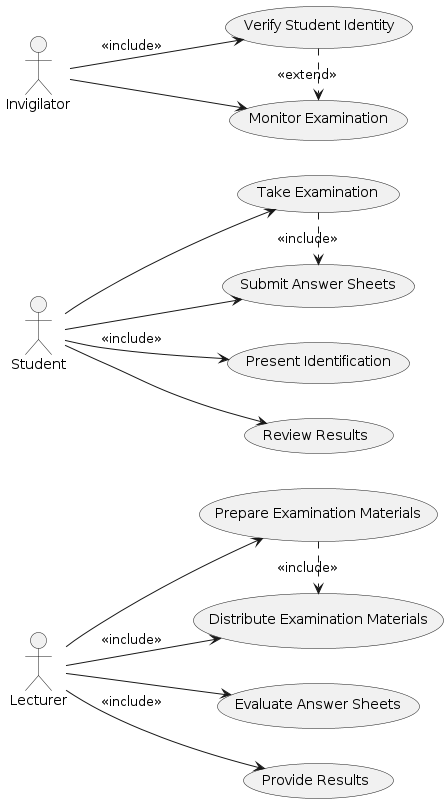
\includegraphics[width=\linewidth]{../figures/usecase_offline_exam}}
	\hfill
	\subcaptionbox{Usecase diagram untuk ujian online.\label{fig:usecase_online_exam}}%
	[0.495\linewidth]{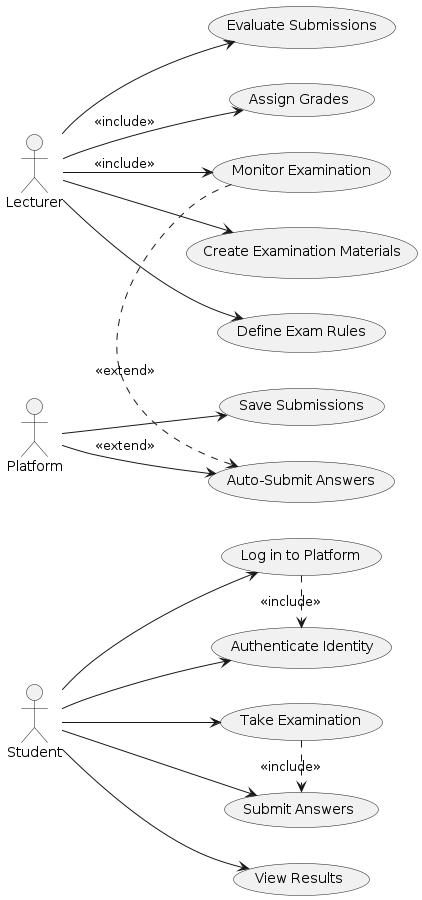
\includegraphics[width=\linewidth]{../figures/usecase_online_exam}}
	\caption{Perbandingan usecase diagram untuk ujian offline dan online.}
\end{figure}

\subsubsection{Sistem Ujian Offline (Baseline)}

Sistem ujian offline mewakili pendekatan tradisional dan manual dalam pelaksanaan ujian. Aktor yang terlibat dalam sistem ini adalah \textbf{Dosen}, \textbf{Mahasiswa}, dan \textbf{Pengawas Ujian}. Interaksi utama antara aktor dan sistem adalah sebagai berikut:

\begin{itemize}
	\item \textbf{Dosen} bertanggung jawab untuk mempersiapkan materi ujian, mendistribusikan materi, mengevaluasi lembar jawaban, dan memberikan hasil. Distribusi materi dan pemberian hasil dimodelkan sebagai hubungan "include", yang menunjukkan bahwa tindakan ini merupakan bagian dari proses yang lebih luas.
	\item \textbf{Mahasiswa} mengikuti ujian, mengumpulkan lembar jawaban, menunjukkan identifikasi untuk verifikasi, dan meninjau hasil ujian. Penyajian identitas dimodelkan sebagai hubungan "include" karena wajib dilakukan untuk mengikuti ujian.
	\item \textbf{Pengawas Ujian} memantau jalannya ujian dan memverifikasi identitas mahasiswa. Proses verifikasi identitas sangat penting dan dimodelkan sebagai hubungan "include". Selain itu, verifikasi identitas memperpanjang proses pemantauan untuk memastikan integritas ujian.
\end{itemize}

Sistem offline, meskipun sudah dikenal, memerlukan intervensi manual di setiap tahap. Alur tugas seperti distribusi, evaluasi, dan verifikasi identitas sangat bergantung pada keterlibatan manusia, yang dapat memakan waktu dan rentan terhadap kesalahan.

\subsubsection{Sistem Ujian Online (Target)}

Sistem ujian online memperkenalkan otomatisasi dan interaksi berbasis platform untuk meningkatkan efisiensi dan skalabilitas. Aktor utama dalam sistem ini adalah \textbf{Dosen}, \textbf{Mahasiswa}, dan \textbf{Platform}. Kegiatan utama dalam sistem ini adalah:

\begin{itemize}
	\item \textbf{Dosen} membuat materi ujian, mendefinisikan aturan ujian, memantau ujian, mengevaluasi kiriman jawaban, dan memberikan nilai. Proses pemantauan mencakup alat otomatis yang disediakan oleh platform untuk meningkatkan efisiensi. Pemberian nilai dimodelkan sebagai hubungan "include" karena merupakan bagian wajib dari evaluasi.
	\item \textbf{Mahasiswa} login ke platform, melakukan autentikasi identitas, mengikuti ujian, mengirim jawaban, dan melihat hasil. Langkah autentikasi sangat penting dalam proses ini, dimodelkan sebagai hubungan "include" untuk memastikan integritas ujian. Pengiriman jawaban juga dimodelkan sebagai tindakan wajib setelah menyelesaikan ujian.
	\item \textbf{Platform} mengotomatiskan beberapa tugas, seperti menyimpan kiriman jawaban dan secara otomatis mengirim jawaban jika mahasiswa tidak melakukannya secara manual sebelum tenggat waktu. Ini dimodelkan sebagai hubungan "extend" untuk menunjukkan bahwa itu terjadi hanya dalam kondisi tertentu (misalnya, waktu habis).
\end{itemize}

Sistem online, dibandingkan dengan yang offline, menawarkan fleksibilitas dan skalabilitas yang lebih besar dengan memungkinkan mahasiswa mengikuti ujian dari jarak jauh dan mengotomatiskan beberapa proses utama, seperti pengiriman dan penilaian. Ini mengurangi beban kerja pada aktor manusia dan memastikan pemantauan ujian yang lebih konsisten melalui kemampuan platform.


\subsection{Activity Diagram}

\begin{figure}[th!]
	\centering
	\subcaptionbox{Activity diagram untuk ujian offline.\label{fig:activity_offline_exam}}%
	[0.49\linewidth]{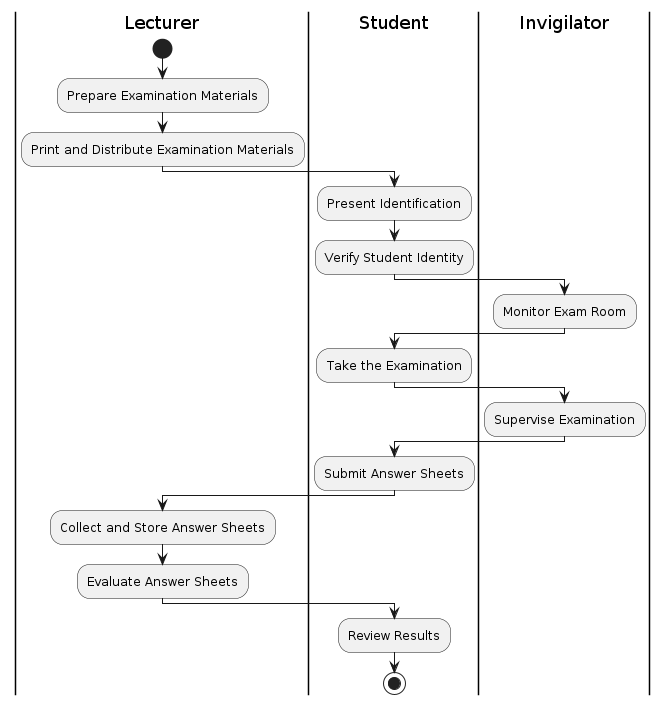
\includegraphics[width=\linewidth]{../figures/activity_offline_exam}}
	\hfill
	\subcaptionbox{Activity diagram untuk ujian online.\label{fig:activity_online_exam}}%
	[0.49\linewidth]{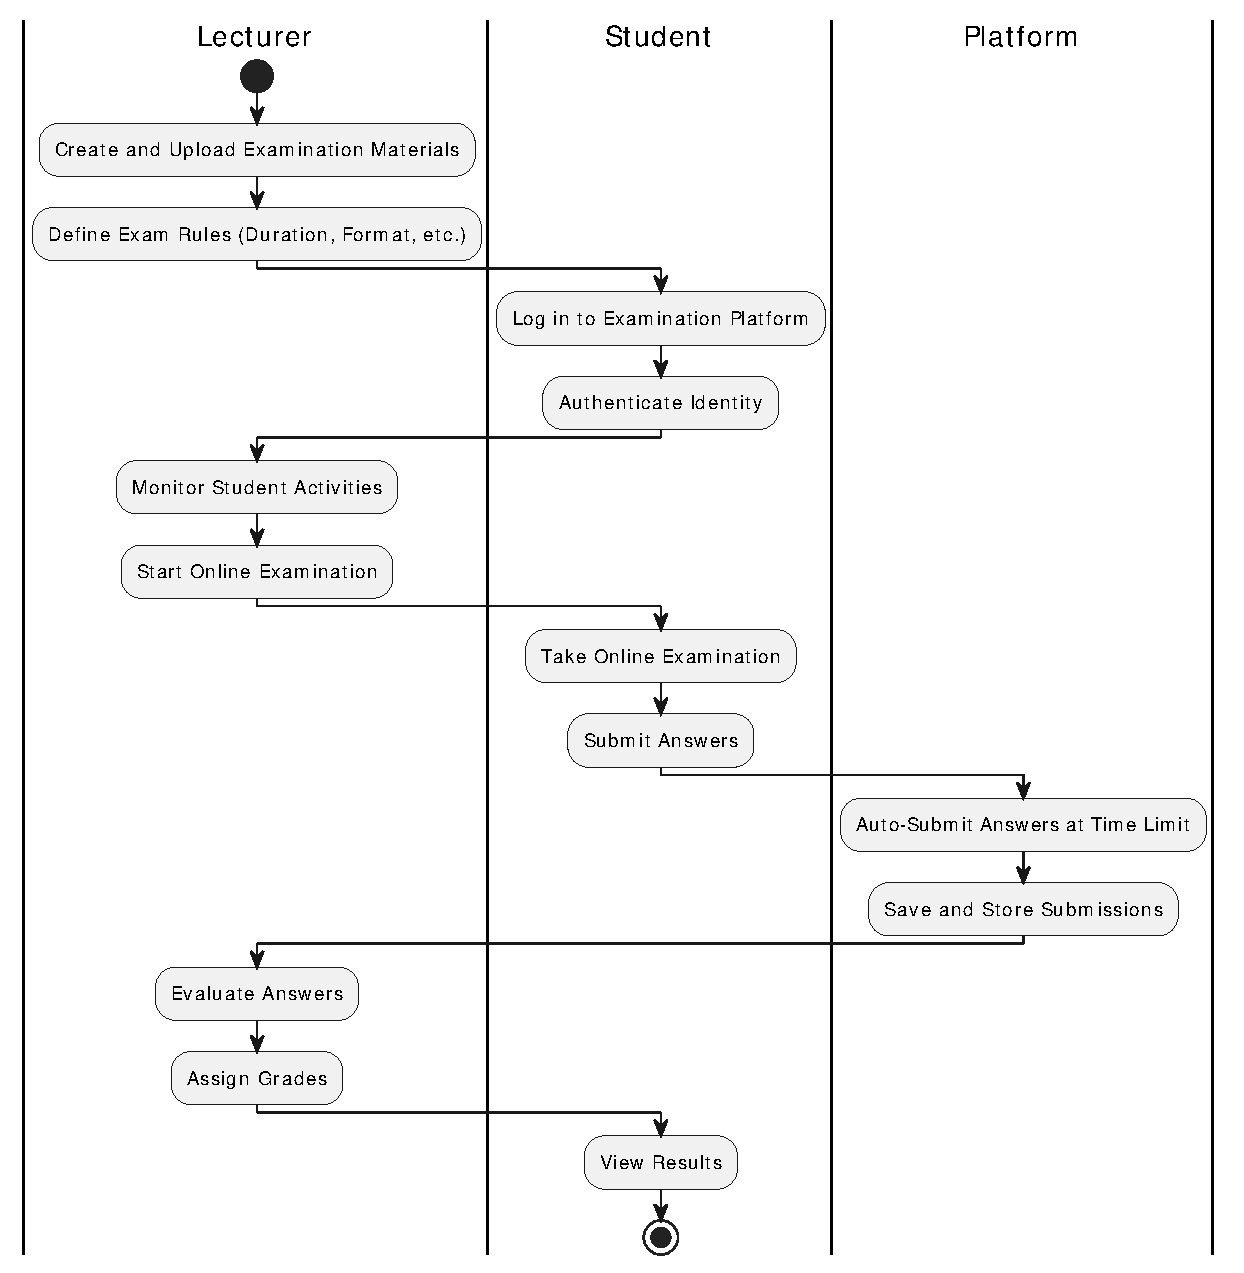
\includegraphics[width=\linewidth]{../figures/activity_online_exam}}
	\caption{Perbandingan activity diagram untuk ujian offline dan online.}
\end{figure}

Activity diagram (Figures \ref{fig:activity_offline_exam} dan \ref{fig:activity_online_exam}) menggambarkan proses ujian pada sistem ujian offline dan online. Setiap diagram menunjukkan alur kerja dari berbagai aktor yang terlibat, seperti dosen, mahasiswa, pengawas, dan platform ujian online.

\subsubsection{Activity Diagram Ujian Offline}

Pada sistem ujian offline, proses ujian dilaksanakan secara manual, mulai dari persiapan hingga evaluasi hasil ujian. Berikut adalah penjelasan dari activity diagram:

\begin{itemize}
	\item \textbf{Dosen} memulai proses dengan mempersiapkan materi ujian, mencetak, dan mendistribusikannya kepada para mahasiswa.
	\item \textbf{Mahasiswa} datang ke ruang ujian dan harus terlebih dahulu menunjukkan identitas diri untuk diverifikasi oleh pengawas. Setelah identitas mahasiswa diverifikasi, mereka dapat mengikuti ujian.
	\item \textbf{Pengawas Ujian} bertanggung jawab untuk memantau ruang ujian selama proses berlangsung, memastikan tidak ada pelanggaran aturan.
	\item Setelah mahasiswa selesai mengerjakan ujian, mereka mengumpulkan lembar jawaban kepada dosen melalui pengawas.
	\item \textbf{Dosen} mengumpulkan, menyimpan, dan kemudian mengevaluasi lembar jawaban tersebut untuk memberikan penilaian.
	\item Setelah proses penilaian selesai, mahasiswa dapat meninjau hasil ujian mereka.
\end{itemize}

Activity diagram ini menunjukkan bahwa setiap tahap dalam proses ujian offline memerlukan interaksi fisik antara mahasiswa, dosen, dan pengawas, serta membutuhkan verifikasi identitas manual dan pengawasan langsung.

\subsubsection{Activity Diagram Ujian Online}

Pada sistem ujian online, banyak aspek dari proses ujian yang diotomatisasi dan difasilitasi oleh platform digital. Berikut adalah penjelasan dari activity diagram:

\begin{itemize}
	\item \textbf{Dosen} memulai dengan membuat dan mengunggah materi ujian ke platform ujian online, serta mendefinisikan aturan ujian, seperti durasi dan format.
	\item \textbf{Mahasiswa} kemudian masuk ke platform ujian online dan melakukan autentikasi identitas sebelum dapat mengikuti ujian.
	\item \textbf{Dosen} memantau aktivitas mahasiswa selama ujian berlangsung dan memulai ujian online sesuai dengan jadwal yang telah ditetapkan.
	\item \textbf{Mahasiswa} mengerjakan ujian di platform, dan jika batas waktu telah tercapai, platform secara otomatis mengirim jawaban yang telah disimpan.
	\item \textbf{Platform} bertanggung jawab untuk menyimpan semua kiriman jawaban yang diunggah oleh mahasiswa, baik secara manual maupun otomatis.
	\item Setelah ujian selesai, \textbf{Dosen} mengevaluasi jawaban dan memberikan penilaian.
	\item \textbf{Mahasiswa} dapat melihat hasil ujian mereka melalui platform setelah penilaian selesai.
\end{itemize}

Activity diagram ini menunjukkan bahwa proses ujian online mengandalkan teknologi untuk mengotomatiskan beberapa tugas penting, seperti autentikasi identitas, pengumpulan jawaban, dan penyimpanan hasil ujian, sehingga mengurangi interaksi fisik dan meningkatkan efisiensi.

\subsection{Archimate Diagram}

\begin{figure}[th!]
	\centering
	\subcaptionbox{Archimate diagram untuk ujian offline.\label{fig:archimate_business_offline_exam}}%
	[0.49\linewidth]{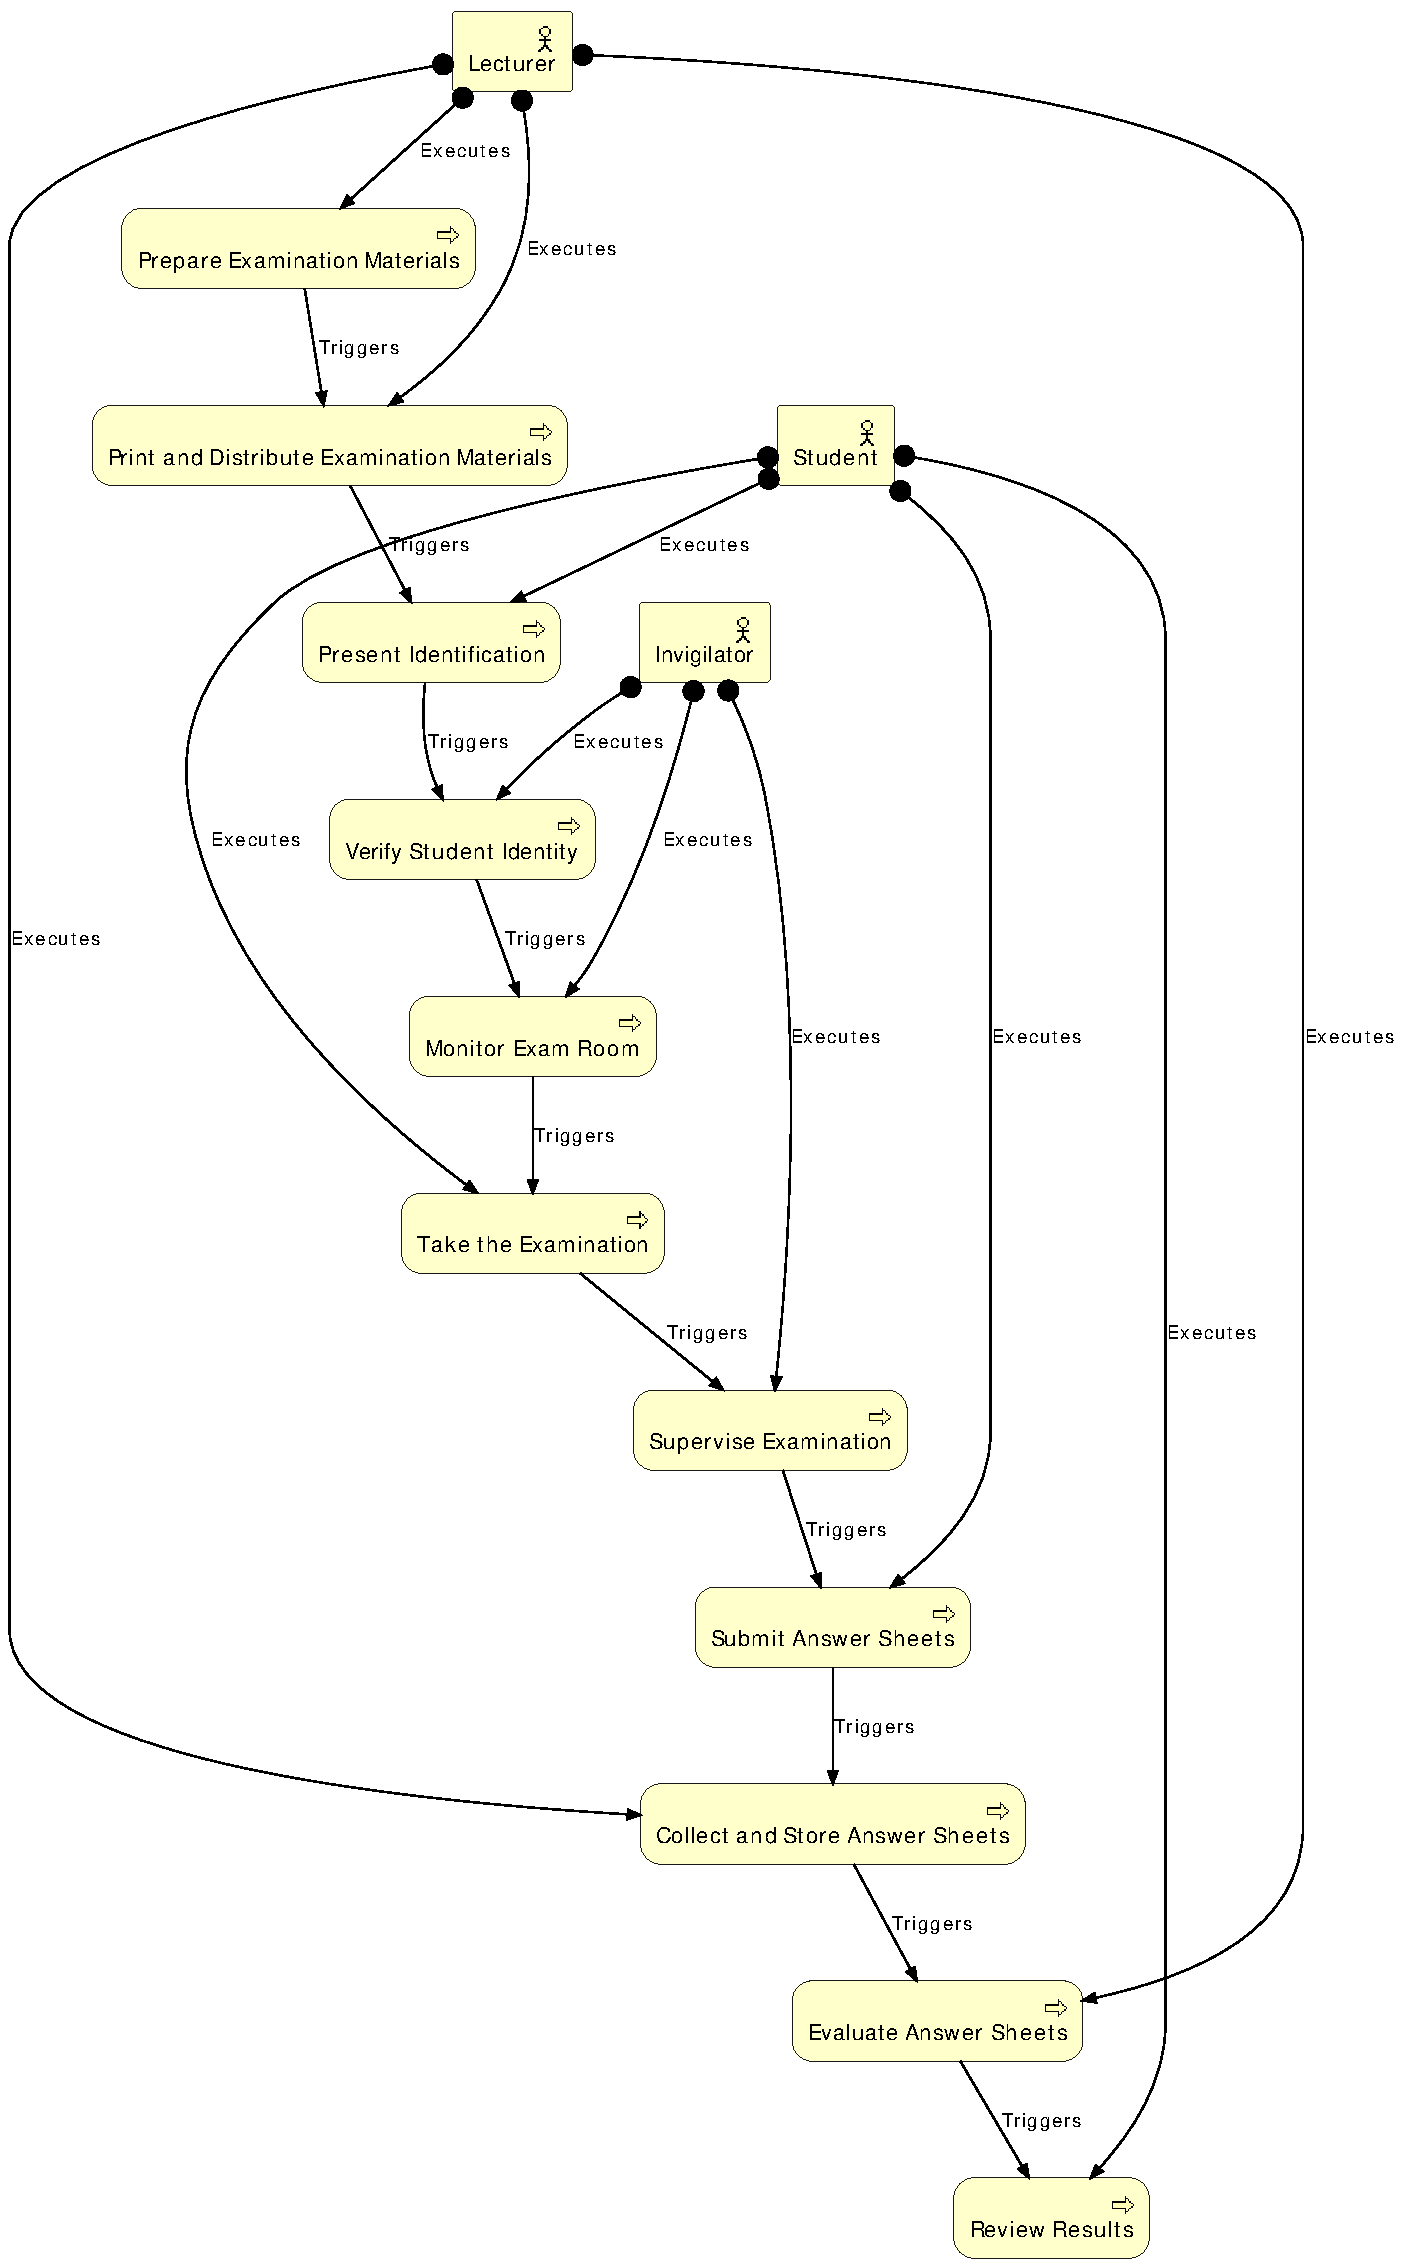
\includegraphics[width=\linewidth]{../figures/archimate_business_offline_exam.pdf}}
	\hfill
	\subcaptionbox{Archimate diagram untuk ujian online.\label{fig:archimate_business_online_exam}}%
	[0.49\linewidth]{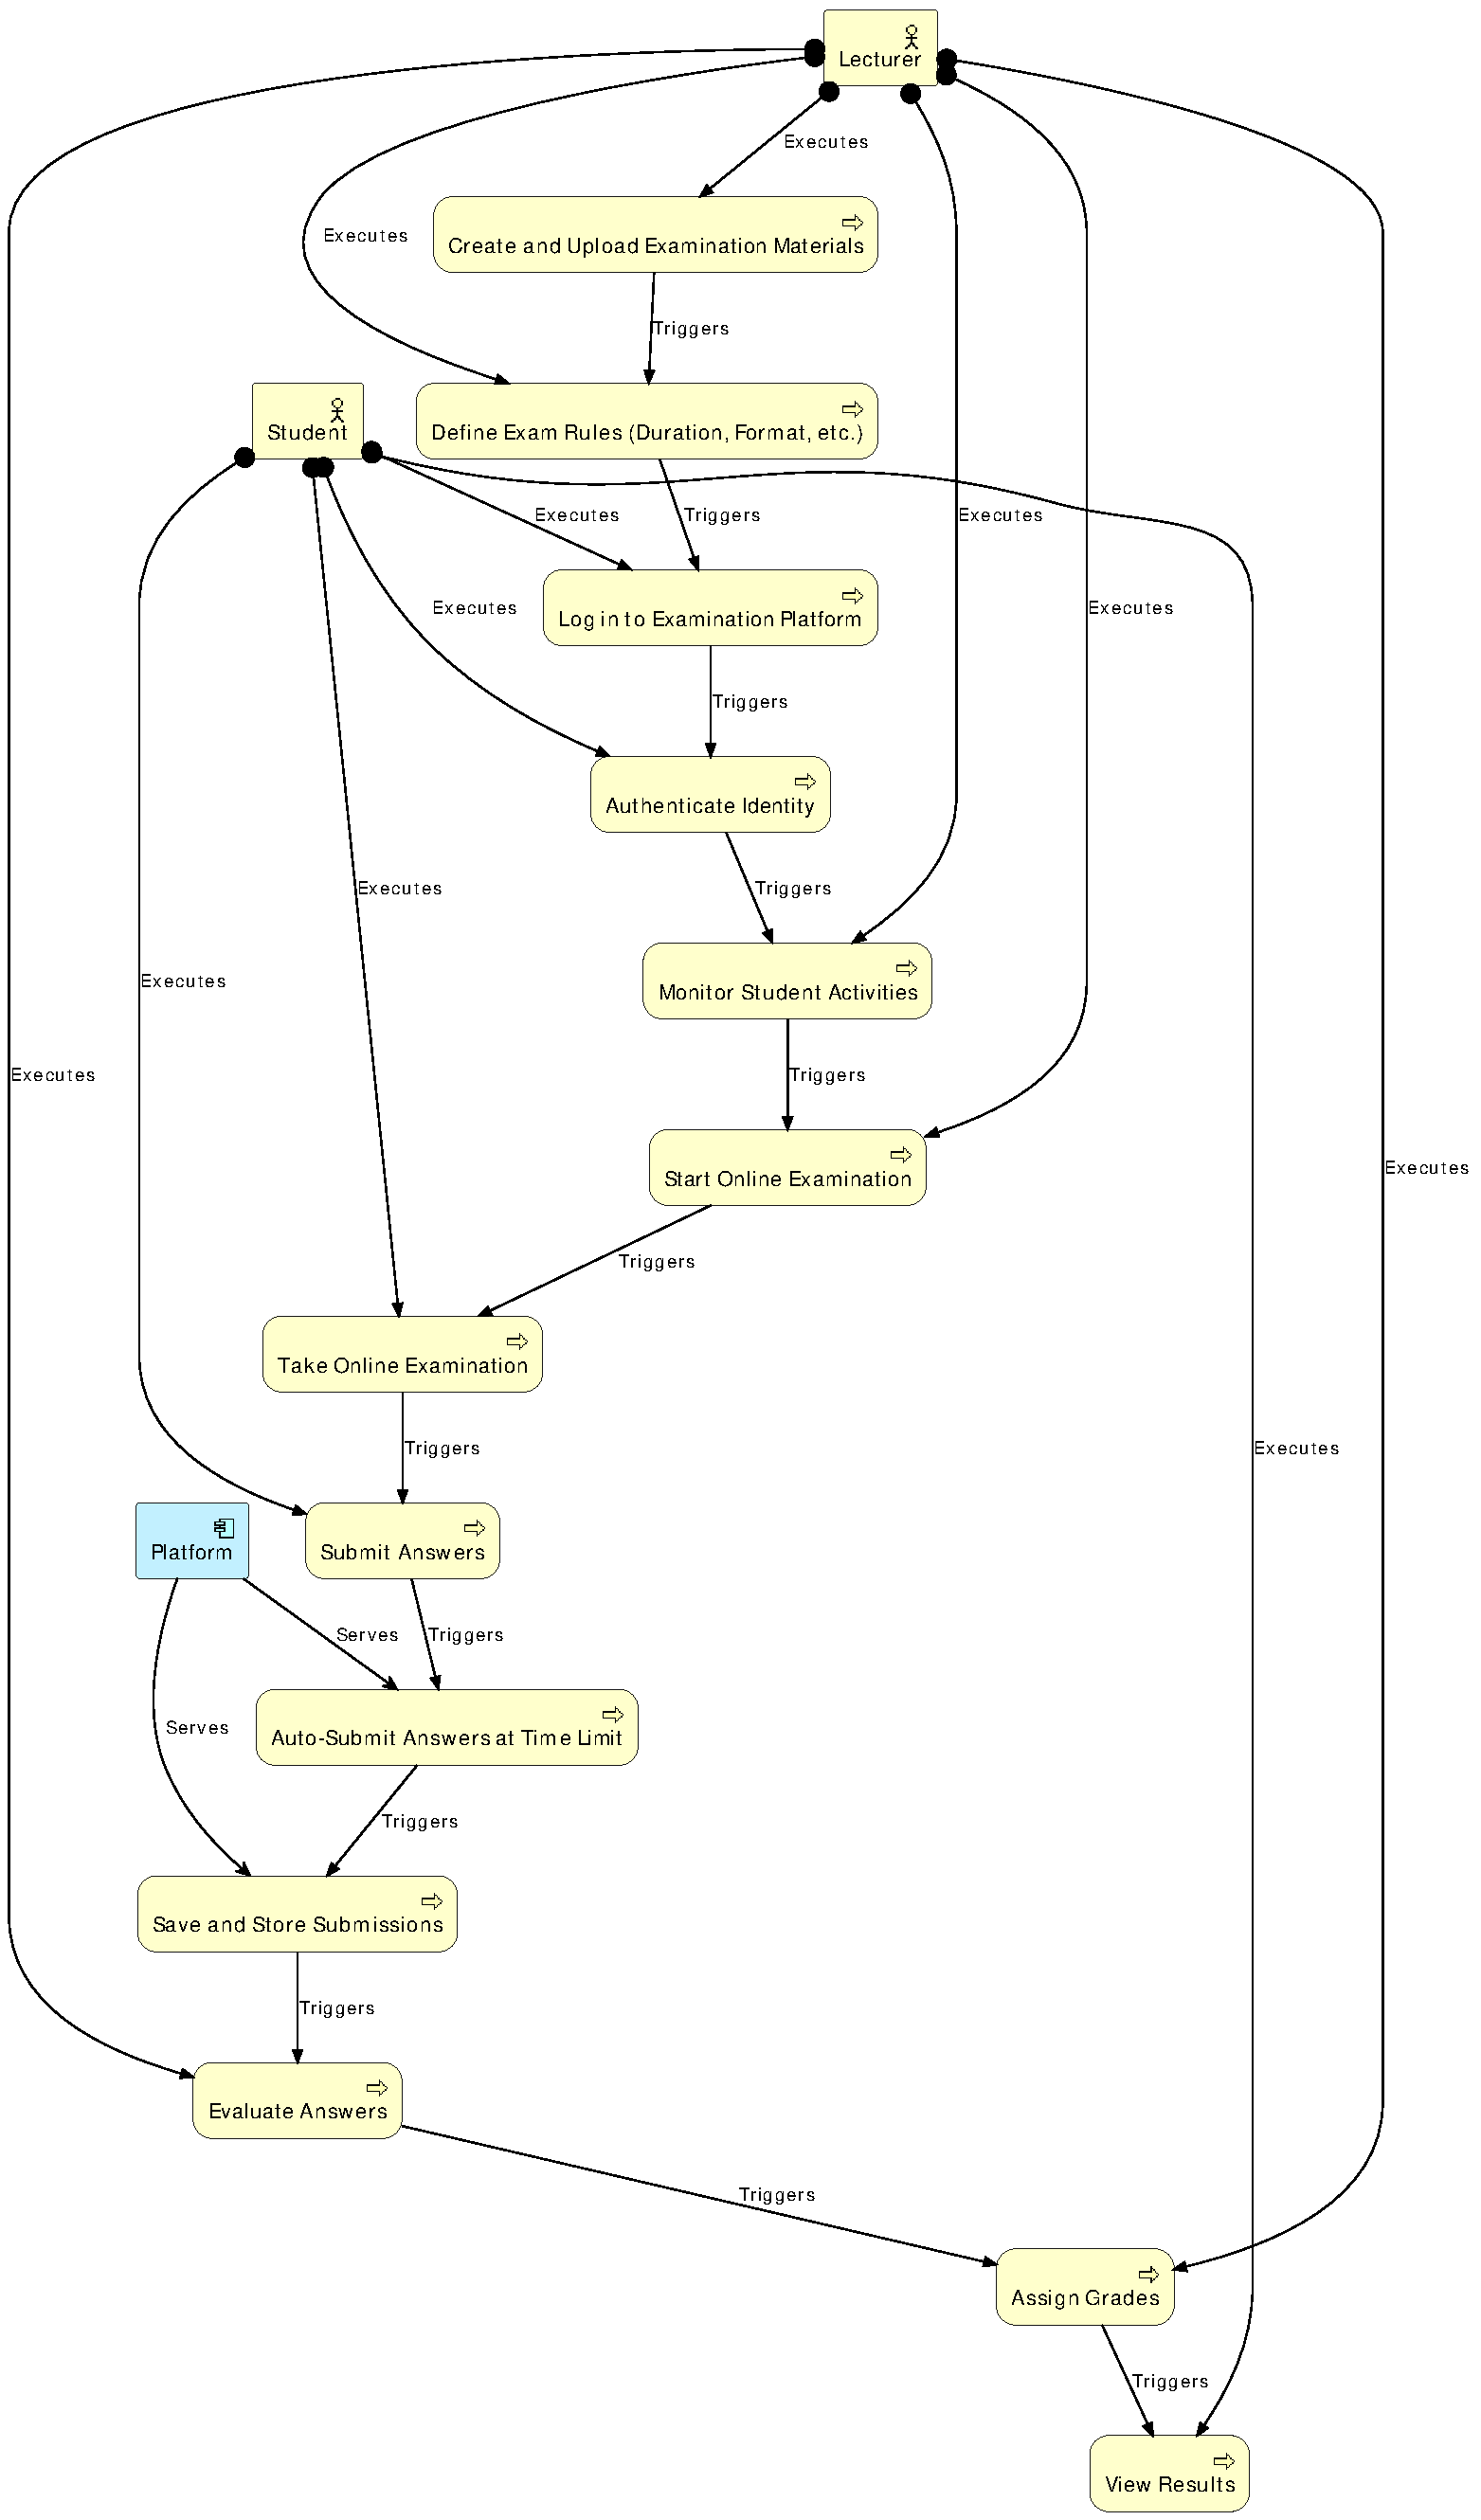
\includegraphics[width=\linewidth]{../figures/archimate_business_online_exam.pdf}}
	\caption{Perbandingan Archimate diagram untuk ujian offline dan online.}
\end{figure}

Pada bagian ini dijelaskan dua ArchiMate diagram yang menggambarkan proses ujian pada sistem ujian offline dan online. Masing-masing diagram menunjukkan alur proses bisnis, aktor yang terlibat, serta hubungan antara proses-proses tersebut.

\subsubsection{ArchiMate Diagram Ujian Offline}

Diagram ArchiMate ujian offline menggambarkan alur proses manual dalam pelaksanaan ujian. Aktor-aktor yang terlibat dalam sistem ini mencakup \textbf{Dosen}, \textbf{Mahasiswa}, dan \textbf{Pengawas Ujian}. Berikut adalah penjelasan detail dari alur proses dalam diagram ini:

\begin{itemize}
	\item \textbf{Dosen} bertanggung jawab untuk mempersiapkan materi ujian, kemudian mencetak dan mendistribusikan materi tersebut kepada mahasiswa.
	\item \textbf{Mahasiswa} harus menunjukkan identifikasi diri sebelum memulai ujian, di mana proses ini diverifikasi oleh pengawas.
	\item \textbf{Pengawas Ujian} bertugas memverifikasi identitas mahasiswa dan memantau ruangan ujian selama ujian berlangsung untuk memastikan kepatuhan terhadap aturan.
	\item Setelah ujian dimulai, \textbf{Mahasiswa} mengerjakan ujian, sementara \textbf{Pengawas} mengawasi jalannya ujian.
	\item Setelah ujian selesai, mahasiswa mengumpulkan lembar jawaban yang kemudian dikumpulkan oleh dosen.
	\item \textbf{Dosen} akan mengevaluasi lembar jawaban dan memberikan hasil kepada mahasiswa untuk ditinjau.
\end{itemize}

Diagram ini menunjukkan alur proses yang ketat dan linear, dengan setiap tahap dalam proses ujian bergantung pada interaksi langsung antara aktor-aktor manusia, serta memerlukan verifikasi manual.

\subsubsection{ArchiMate Diagram Ujian Online}

Diagram ArchiMate ujian online menggambarkan sistem ujian yang difasilitasi oleh platform digital dengan banyak proses yang diotomatisasi. Aktor yang terlibat dalam diagram ini mencakup \textbf{Dosen}, \textbf{Mahasiswa}, dan \textbf{Platform} sebagai komponen aplikasi. Berikut adalah penjelasan prosesnya:

\begin{itemize}
	\item \textbf{Dosen} membuat dan mengunggah materi ujian ke platform, kemudian mendefinisikan aturan ujian seperti durasi dan format ujian.
	\item \textbf{Mahasiswa} masuk ke platform ujian dan mengautentikasi identitas mereka sebelum dapat mengikuti ujian.
	\item Selama ujian berlangsung, \textbf{Dosen} memantau aktivitas mahasiswa melalui platform, dan memulai ujian secara online.
	\item \textbf{Mahasiswa} mengikuti ujian melalui platform, di mana jawaban dapat diserahkan secara manual atau secara otomatis oleh \textbf{Platform} saat batas waktu tercapai.
	\item Platform juga bertanggung jawab untuk menyimpan kiriman jawaban secara otomatis, sementara \textbf{Dosen} mengevaluasi jawaban yang telah disimpan dan memberikan penilaian.
	\item Setelah penilaian selesai, \textbf{Mahasiswa} dapat melihat hasil ujian mereka melalui platform.
\end{itemize}

Diagram ini menekankan peran teknologi dalam mengotomatiskan beberapa proses penting, seperti autentikasi identitas, penyimpanan jawaban, dan pemantauan ujian, yang mengurangi keterlibatan langsung manusia dan meningkatkan efisiensi proses ujian.

Sistem ujian offline memerlukan interaksi langsung antara dosen, mahasiswa, dan pengawas, serta membutuhkan banyak proses manual yang memakan waktu dan rentan terhadap kesalahan. Sebaliknya, sistem ujian online menawarkan otomatisasi yang lebih tinggi dengan platform yang menangani banyak tugas seperti autentikasi, pemantauan, dan penyimpanan jawaban. Hal ini tidak hanya meningkatkan efisiensi tetapi juga memberikan fleksibilitas yang lebih besar bagi dosen dan mahasiswa.


\subsection{Analisis Keuntungan dan Kerugian}

\textbf{Offline (Baseline)}

\textbf{Keuntungan:}
\begin{enumerate}
	\item Proses yang sudah dikenal: Prosedur ujian tradisional yang melibatkan materi fisik dan pengawasan manusia sudah dipahami dengan baik oleh dosen, mahasiswa, dan pengawas.
	\item Pengawasan langsung: Dosen dan pengawas dapat memantau perilaku mahasiswa secara langsung, memungkinkan intervensi segera jika terjadi masalah, seperti kecurangan.
	\item Tidak bergantung pada teknologi: Pendekatan ini tidak mengandalkan platform perangkat lunak, sehingga mengurangi kekhawatiran tentang kegagalan teknis atau keamanan sistem.
\end{enumerate}

\textbf{Kerugian:}
\begin{enumerate}
	\item Memakan waktu: Mempersiapkan, mendistribusikan, dan mengevaluasi materi fisik adalah proses manual yang memerlukan waktu yang cukup lama bagi dosen dan staf administrasi.
	\item Rentan terhadap kesalahan manusia: Proses manual seperti penilaian atau verifikasi identitas mahasiswa dapat menyebabkan ketidakakuratan.
	\item Skalabilitas terbatas: Penanganan ujian untuk jumlah mahasiswa yang besar menjadi tantangan logistik.
	\item Aksesibilitas terbatas: Mahasiswa harus hadir secara fisik untuk mengikuti ujian, yang dapat membatasi fleksibilitas, terutama dalam lingkungan pembelajaran jarak jauh atau hybrid.
\end{enumerate}

\textbf{Online (Target)}

\textbf{Keuntungan:}
\begin{enumerate}
	\item Efisiensi: Proses persiapan dan evaluasi ujian dapat diotomatiskan, dan pengumpulan serta penilaian jawaban dapat dilakukan dengan lebih efisien.
	\item Skalabilitas: Platform digital dapat dengan mudah menangani ujian skala besar, sehingga mengurangi tantangan logistik dari distribusi materi ujian fisik.
	\item Aksesibilitas: Mahasiswa dapat mengikuti ujian dari jarak jauh, yang mendukung model pembelajaran hybrid atau sepenuhnya online.
	\item Manajemen data: Platform secara aman menyimpan kiriman jawaban dan data autentikasi identitas, memberikan proses yang terstruktur dan transparan.
	\item Tindakan otomatis: Fitur seperti pengiriman jawaban otomatis mengurangi risiko mahasiswa kehilangan pekerjaan karena masalah teknis atau batasan waktu.
\end{enumerate}

\textbf{Kerugian:}
\begin{enumerate}
	\item Ketergantungan pada teknologi: Sistem ini sangat bergantung pada ketersediaan dan keandalan platform online, yang dapat mengganggu proses ujian jika terjadi masalah teknis.
	\item Kekhawatiran keamanan: Autentikasi dan pencegahan kecurangan memerlukan langkah-langkah kuat untuk memastikan integritas ujian, yang mungkin memerlukan biaya tambahan.
	\item Kurva belajar: Baik mahasiswa maupun dosen perlu membiasakan diri dengan platform, dan beberapa mungkin menghadapi tantangan dalam beradaptasi dengan teknologi.
\end{enumerate}

\subsection{Analisis Upaya yang Diperlukan untuk Migrasi dari Sistem Ujian Offline (Baseline) ke Online (Target)}

\begin{enumerate}
	
	\item \textbf{Pemilihan dan Penyiapan Platform}
	\begin{enumerate}
		\item Melakukan penelitian dan evaluasi platform ujian online yang memenuhi kebutuhan institusi, dengan fokus pada keamanan, skalabilitas, dan kemudahan penggunaan.
		\item Memperoleh teknologi yang diperlukan, termasuk lisensi platform dan perangkat yang kompatibel dengan sistem.
		\item Mengintegrasikan platform baru dengan sistem informasi mahasiswa (SIS) yang sudah ada untuk mengelola data mahasiswa dan informasi mata kuliah secara efektif.
	\end{enumerate}
	
	\item \textbf{Persiapan dan Konversi Konten}
	\begin{enumerate}
		\item Mengonversi materi ujian yang ada (soal, rubrik penilaian, dll.) ke dalam format digital yang kompatibel dengan platform online.
		\item Mengonfigurasi ujian online di dalam platform, termasuk pengaturan bank soal, aturan ujian, dan kriteria penilaian.
	\end{enumerate}
	
	\item \textbf{Keamanan dan Autentikasi}
	\begin{enumerate}
		\item Mengimplementasikan mekanisme autentikasi yang aman, seperti autentikasi multi-faktor (MFA) atau pengenalan wajah, untuk verifikasi identitas mahasiswa.
		\item Mengintegrasikan alat pengawasan ujian, seperti perangkat lunak proctoring, untuk memantau mahasiswa dan mencegah kecurangan selama ujian.
	\end{enumerate}
	
	\item \textbf{Pelatihan dan Pembiasaan}
	\begin{enumerate}
		\item Memberikan pelatihan kepada dosen tentang cara membuat, memantau, dan menilai ujian menggunakan platform baru.
		\item Menawarkan sesi pelatihan untuk mahasiswa tentang cara login, autentikasi, mengikuti ujian, dan mengirim jawaban di platform.
	\end{enumerate}
	
	\item \textbf{Dukungan Teknis dan Pengujian}
	\begin{enumerate}
		\item Mendirikan tim dukungan teknis khusus untuk membantu mahasiswa dan dosen selama proses ujian.
		\item Melakukan ujian percobaan dengan kelompok kecil mahasiswa dan dosen untuk menguji platform dan mengatasi masalah sebelum implementasi penuh.
	\end{enumerate}
	
	\item \textbf{Komunikasi dan Adaptasi Kebijakan}
	\begin{enumerate}
		\item Menyesuaikan kebijakan ujian yang ada agar sesuai dengan lingkungan online, termasuk aturan tentang verifikasi identitas dan integritas akademik.
		\item Mengkomunikasikan rencana migrasi, kebijakan baru, dan prosedur kepada semua pihak terkait—dosen, mahasiswa, dan staf administrasi—jauh sebelum periode ujian dimulai.
	\end{enumerate}
	
	\item \textbf{Pemantauan dan Iterasi}
	\begin{enumerate}
		\item Secara aktif memantau kinerja platform selama ujian dan memberikan dukungan secara real-time jika diperlukan.
		\item Mengumpulkan umpan balik dari mahasiswa dan dosen setelah ujian untuk meningkatkan proses pada periode ujian berikutnya.
	\end{enumerate}
	
\end{enumerate}

\subsection{Analisis Biaya-Manfaat}

\subsubsection{Biaya}
\begin{enumerate}
	\item Biaya pengaturan awal: Pembelian platform ujian online, termasuk biaya lisensi dan integrasi.
	\item Pelatihan: Waktu dan sumber daya yang digunakan untuk melatih staf dan mahasiswa dalam menggunakan platform baru.
	\item Biaya pemeliharaan: Pengeluaran berkelanjutan untuk memelihara dan mendukung platform, termasuk dukungan teknis.
	\item Manajemen risiko: Investasi tambahan dalam infrastruktur TI atau solusi keamanan untuk mengatasi masalah seperti waktu henti sistem atau pencegahan kecurangan.
\end{enumerate}

\subsubsection{Manfaat}
\begin{enumerate}
	\item Penghematan waktu: Otomatisasi mengurangi beban kerja manual dalam mempersiapkan ujian, menilai jawaban, dan mengelola kiriman.
	\item Skalabilitas: Platform dapat mengakomodasi lebih banyak mahasiswa tanpa meningkatkan beban pada dosen dan staf administrasi.
	\item Aksesibilitas: Mahasiswa dapat mengikuti ujian dari lokasi jarak jauh, meningkatkan fleksibilitas dan mendukung model pembelajaran hybrid.
	\item Manajemen data yang lebih baik: Penyimpanan digital untuk kiriman ujian dan data penilaian memastikan organisasi dan transparansi yang lebih baik.
	\item Umpan balik lebih cepat: Penilaian otomatis memungkinkan mahasiswa menerima umpan balik lebih cepat, yang meningkatkan proses pembelajaran.
\end{enumerate}

Meskipun biaya awal untuk pengaturan sistem ujian online signifikan, manfaat jangka panjang—termasuk penghematan waktu, skalabilitas, dan fleksibilitas—menjadikan transisi ini berharga. Sistem online juga mendukung pembelajaran hybrid, membuatnya menjadi solusi berkelanjutan untuk pendidikan modern.


\section{Aktivitas Kelas dan Tugas}

Buatlah arsitektur bisnis \textbf{As-Is} yang terdampak oleh kapabilitas arsitektur yang dipilih. Juga, buat arsitektur bisnis \textbf{To-Be} yang diperlukan untuk mewujudkan kapabilitas tersebut. 
Expresikan arsitektur bisnis \textbf{As-Is} dan \textbf{To-Be} dalam bentuk Dokumen Definisi Arsitektur (Subbab \ref{sec:isi_dokumen_definisi_arsitektur}) dan Spesifikasi Persyaratan Arsitektur (Subbab \ref{sec:spesifikasi_kebutuhan_arsitektur}).

	\chapter{Arsitektur Data}

\section{Tujuan}
Tujuan dari fase ini adalah untuk mengembangkan Arsitektur Data Target yang memungkinkan Arsitektur Bisnis dan Visi Arsitektur dapat tercapai, sambil menangani Permintaan Pekerjaan Arsitektur dan \textit{concerns} dari para \textit{stakeholder}. Selain itu, fase ini bertujuan untuk mengidentifikasi komponen Peta Jalan Arsitektur berdasarkan kesenjangan antara Arsitektur Data Dasar dan Arsitektur Data Target.

\section{Input (1)}
Input yang digunakan dalam fase ini meliputi:
\begin{enumerate}
	\item Permintaan Pekerjaan Arsitektur
	\item Penilaian Kapabilitas
	\item Rencana Komunikasi
	\item Model Organisasi untuk Arsitektur Perusahaan
	\item Kerangka Kerja Arsitektur yang Disesuaikan
	\item Prinsip Data, jika ada
	\item Pernyataan Pekerjaan Arsitektur
	\item Draf Spesifikasi Kebutuhan Arsitektur, mencakup:
	\begin{enumerate}
		\item Hasil Analisis Kesenjangan
		\item Kebutuhan teknis relevan lainnya
	\end{enumerate}
	\item Visi Arsitektur
	\item Repositori Arsitektur
	\item Draf Dokumen Definisi Arsitektur, mencakup:
	\begin{enumerate}
		\item Arsitektur Bisnis Dasar (rinci)
		\item Arsitektur Bisnis Target (rinci)
		\item Arsitektur Data Dasar (garis besar)
		\item Arsitektur Data Target (garis besar)
		\item Arsitektur Aplikasi Dasar (garis besar)
		\item Arsitektur Aplikasi Target (garis besar)
		\item Arsitektur Teknologi Dasar (garis besar)
		\item Arsitektur Teknologi Target (garis besar)
	\end{enumerate}
	\item Komponen Arsitektur Bisnis dari Peta Jalan Arsitektur
\end{enumerate}

\section{Langkah-langkah}
Langkah-langkah yang diambil dalam fase ini meliputi:
\begin{enumerate}
	\item Memilih model referensi, sudut pandang, dan alat
	\item Mengembangkan Deskripsi Arsitektur Data Dasar
	\item Mengembangkan Deskripsi Arsitektur Data Target
	\item Melakukan Analisis Kesenjangan
	\item Menentukan komponen peta jalan kandidat
	\item Menyelesaikan dampak pada Lanskap Arsitektur
	\item Melakukan tinjauan formal dari pemangku kepentingan
	\item Menyelesaikan Arsitektur Data
	\item Membuat Dokumen Definisi Arsitektur
\end{enumerate}

\subsection*{Contoh:}
Langkah-langkah yang diambil dalam fase ini meliputi:
\begin{enumerate}
	\item Memilih model referensi, sudut pandang, dan alat
	\begin{itemize}
		\item Contoh: Memilih model referensi pedagogis seperti Community of Inquiry (CoI) untuk pembelajaran hybrid, dengan sudut pandang dari dosen dan mahasiswa, serta alat seperti Moodle atau Google Classroom untuk manajemen kursus.
	\end{itemize}
	\item Mengembangkan Deskripsi Arsitektur Data \textit{Baseline}
	\begin{itemize}
		\item Contoh: Membuat peta data yang mencakup informasi tentang interaksi mahasiswa dalam lingkungan belajar daring dan luring, seperti data kehadiran dan partisipasi dalam diskusi.
	\end{itemize}
	\item Mengembangkan Deskripsi Arsitektur Data Target
	\begin{itemize}
		\item Contoh: Merancang sistem yang mendukung analitik pembelajaran untuk mengevaluasi keterlibatan dan kemajuan mahasiswa, termasuk pengintegrasian data dari platform pembelajaran dan sistem manajemen akademik.
	\end{itemize}
	\item Melakukan Analisis Kesenjangan
	\begin{itemize}
		\item Contoh: Menganalisis kesenjangan antara praktik pengajaran saat ini dan kebutuhan untuk model pembelajaran hybrid, seperti kurangnya data tentang keterlibatan mahasiswa dalam sesi tatap muka versus daring.
	\end{itemize}
	\item Menentukan komponen peta jalan kandidat
	\begin{itemize}
		\item Contoh: Mengidentifikasi proyek-proyek pengembangan kursus hybrid, seperti pelatihan dosen dalam penggunaan teknologi pembelajaran dan pengembangan materi pembelajaran yang dapat diakses secara daring.
	\end{itemize}
	\item Menyelesaikan dampak pada Lanskap Arsitektur
	\begin{itemize}
		\item Contoh: Menganalisis dampak transisi ke pembelajaran hybrid pada infrastruktur TI universitas dan kesiapan dosen untuk mengajar dalam format ini.
	\end{itemize}
	\item Melakukan tinjauan formal dari pemangku kepentingan
	\begin{itemize}
		\item Contoh: Mengadakan forum diskusi dengan dosen, mahasiswa, dan staf administrasi untuk meninjau arsitektur pembelajaran hybrid dan mengumpulkan masukan tentang tantangan yang dihadapi.
	\end{itemize}
	\item Menyelesaikan Arsitektur Data
	\begin{itemize}
		\item Contoh: Finalisasi desain arsitektur data yang mendukung evaluasi efektivitas pembelajaran hybrid dengan memperhitungkan umpan balik dari pemangku kepentingan dan analisis data yang ada.
	\end{itemize}
	\item Membuat Dokumen Definisi Arsitektur
	\begin{itemize}
		\item Contoh: Menyusun dokumen definisi arsitektur yang merinci struktur dan proses pembelajaran hybrid, kebijakan penggunaan teknologi, dan protokol untuk mengukur hasil pembelajaran.
	\end{itemize}
\end{enumerate}


\section{Output}
Output dari fase ini mencakup:
\begin{enumerate}
	\item Pernyataan Pekerjaan Arsitektur, diperbarui sesuai kebutuhan
	\item Prinsip-prinsip data yang divalidasi, atau prinsip-prinsip data baru
	\item Draf Dokumen Definisi Arsitektur dengan konten yang diperbarui
	\item Spesifikasi Kebutuhan Arsitektur yang telah didesain, termasuk yang telah diperbarui
	\item Komponen Arsitektur Data dari Peta Jalan Arsitektur
\end{enumerate}

\subsection{Output}
Output dari fase ini mencakup:
\begin{enumerate}
	\item Pernyataan Pekerjaan Arsitektur, diperbarui sesuai kebutuhan
	\begin{itemize}
		\item Contoh: Dokumen Pernyataan Pekerjaan Arsitektur yang merinci tanggung jawab dan tugas tim dalam mengembangkan lingkungan belajar hybrid, termasuk penyesuaian terhadap kebutuhan teknologi yang muncul selama proses pengajaran.
	\end{itemize}
	\item Prinsip-prinsip data yang divalidasi, atau prinsip-prinsip data baru
	\begin{itemize}
		\item Contoh: Prinsip data yang divalidasi untuk menjaga kerahasiaan data mahasiswa dan memastikan aksesibilitas konten pembelajaran secara adil, serta penambahan prinsip baru mengenai penggunaan data analitik untuk meningkatkan pengalaman belajar mahasiswa.
	\end{itemize}
	\item Draf Dokumen Definisi Arsitektur dengan konten yang diperbarui
	\begin{itemize}
		\item Contoh: Draf Dokumen Definisi Arsitektur yang mencakup detail terbaru mengenai platform pembelajaran yang digunakan, prosedur pengajaran hybrid, dan mekanisme evaluasi yang terintegrasi antara pembelajaran daring dan luring.
	\end{itemize}
	\item Spesifikasi Kebutuhan Arsitektur yang telah didesain, termasuk yang telah diperbarui
	\begin{itemize}
		\item Contoh: Spesifikasi kebutuhan yang mencakup alat dan teknologi yang diperlukan untuk mendukung pembelajaran hybrid, seperti perangkat lunak untuk pengelolaan kursus dan sistem umpan balik mahasiswa yang efektif.
	\end{itemize}
	\item Komponen Arsitektur Data dari Peta Jalan Arsitektur
	\begin{itemize}
		\item Contoh: Komponen arsitektur data yang menggambarkan struktur sistem penyimpanan data untuk pembelajaran hybrid, termasuk database untuk menyimpan catatan kehadiran, partisipasi dalam diskusi, dan hasil evaluasi, serta integrasi data dari berbagai platform yang digunakan.
	\end{itemize}
\end{enumerate}

\section{Prinsip Data}
Beberapa prinsip data yang dipegang dalam fase ini adalah:
\begin{enumerate}
	\item \textbf{Data adalah Aset}. Data adalah aset yang memiliki nilai bagi perusahaan dan dikelola sesuai dengan itu.
	\item \textbf{Data dapat dibagikan}. Pengguna dapat mengakses data yang diperlukan untuk melaksanakan tugas mereka; oleh karena itu, data dibagikan di seluruh fungsi dan organisasi perusahaan.
	\item \textbf{Data yang dapat diakses}. Data dapat diakses oleh pengguna untuk menjalankan fungsi mereka.
	\item \textbf{Definisi Kosakata dan Data yang Dibagikan}. Data didefinisikan secara konsisten di seluruh perusahaan, dan definisi tersebut dapat dipahami serta tersedia untuk semua pengguna.
	\item \textbf{Keamanan Data}. Data dilindungi dari penggunaan dan pengungkapan yang tidak sah. Selain aspek tradisional dari klasifikasi keamanan nasional, ini termasuk tetapi tidak terbatas pada perlindungan sebelum keputusan, informasi sensitif, pemilihan sumber sensitif, dan informasi kepemilikan.
\end{enumerate}

\section{Katalog, Matriks, dan Diagram Arsitektur Data}
Dalam fase ini, berbagai katalog, matriks, dan diagram yang digunakan meliputi:
\begin{table}[ht]
	\begin{tabular}{|c|c|c|}
		\hline
		\textbf{Katalog} & \textbf{Matriks} & \textbf{Diagram} \\ \hline
		Katalog Entitas Data/Komponen & Matriks Entitas Data/Fungsi Bisnis & Diagram Data Konseptual \\
		& Matriks Aplikasi/Data & Diagram Data Logis \\
		& & Diagram Penyebaran Data \\
		& & Diagram Siklus Hidup Data \\
		& & Diagram Keamanan Data \\
		& & Diagram Migrasi Data \\ \hline
	\end{tabular}
\end{table}

\section{Komponen Dokumen Definisi Arsitektur}
\label{sec:dokumen_definisi_arsitektur_data}
Topik yang harus dibahas dalam Dokumen Definisi Arsitektur yang terkait dengan Arsitektur Data adalah sebagai berikut:
\begin{itemize}
	\item Arsitektur Data Baseline, jika memungkinkan
	\item Arsitektur Data Target, termasuk model untuk data bisnis, data logis, dan proses manajemen data, serta matriks Entitas Data/Fungsi Bisnis
	\item Pandangan Arsitektur Data yang sesuai dengan sudut pandang yang dipilih, yang mengatasi kekhawatiran pemangku kepentingan kunci
\end{itemize}

\subsection*{Contoh:}
\begin{itemize}
	\item \textbf{Arsitektur Data Baseline, jika memungkinkan} \\
	Contoh: Pada fase awal implementasi hybrid learning, universitas mengumpulkan data mengenai penggunaan platform pembelajaran daring (LMS) dan kehadiran mahasiswa dalam pertemuan tatap muka. Data baseline ini mencakup statistik tentang frekuensi akses mahasiswa ke materi pembelajaran, tingkat partisipasi dalam diskusi online, dan kehadiran dalam kelas fisik. 
	
	\item \textbf{Arsitektur Data Target, termasuk model untuk data bisnis, data logis, dan proses manajemen data, serta matriks Entitas Data/Fungsi Bisnis} \\
	Contoh: Universitas menetapkan Arsitektur Data Target yang mencakup model untuk pengelolaan data mahasiswa, dosen, dan kurikulum. Model ini memetakan hubungan antara entitas seperti mahasiswa, kursus, dan dosen. Misalnya, matriks Entitas Data/Fungsi Bisnis menunjukkan bagaimana data tentang mahasiswa (seperti nilai dan kehadiran) digunakan untuk meningkatkan pengalaman belajar dalam konteks hybrid, misalnya, melalui pengembangan materi yang sesuai untuk pembelajaran daring dan tatap muka.
	
	\item \textbf{Pandangan Arsitektur Data yang sesuai dengan sudut pandang yang dipilih, yang mengatasi kekhawatiran pemangku kepentingan kunci} \\
	Contoh: Dalam konteks hybrid learning, pandangan arsitektur data mencakup perspektif pemangku kepentingan seperti mahasiswa, dosen, dan pengelola pendidikan. Misalnya, mahasiswa mungkin mengkhawatirkan aksesibilitas materi pembelajaran secara daring, sedangkan dosen mungkin fokus pada bagaimana data kehadiran dan partisipasi dapat membantu mereka dalam menyesuaikan metode pengajaran. Pandangan ini diintegrasikan ke dalam laporan analisis untuk memastikan bahwa semua kebutuhan dan kekhawatiran dipertimbangkan dalam pengembangan arsitektur data.
\end{itemize}

\section{Komponen Spesifikasi Kebutuhan Arsitektur}
\label{sec:spesifikasi_kebutuhan_arsitektur_data}
Kebutuhan Arsitektur Data yang mengisi Spesifikasi Kebutuhan Arsitektur pada Fase C meliputi:
\begin{itemize}
	\item Hasil Analisis Kesenjangan
	\item Kebutuhan interoperabilitas data (misalnya, skema XML, kebijakan keamanan)
	\item Area di mana Arsitektur Bisnis mungkin perlu berubah untuk mematuhi perubahan dalam Arsitektur Data
	\item Pembatasan pada Arsitektur Teknologi yang akan dirancang
	\item Kebutuhan bisnis yang telah diperbarui, jika ada
	\item Kebutuhan aplikasi yang telah diperbarui, jika ada
\end{itemize}

\begin{itemize}
	\item \textbf{Hasil Analisis Kesenjangan} \\
	Contoh: Setelah menganalisis data penggunaan LMS, ditemukan bahwa terdapat kesenjangan antara materi yang disediakan secara daring dan kebutuhan mahasiswa dalam kelas tatap muka. Hasil analisis ini menunjukkan perlunya pengembangan materi tambahan yang dapat diakses secara daring untuk mendukung pemahaman mahasiswa.
	
	\item \textbf{Kebutuhan interoperabilitas data (misalnya, skema XML, kebijakan keamanan)} \\
	Contoh: Dalam konteks hybrid learning, kebutuhan interoperabilitas data mencakup penggunaan format data standar seperti skema XML untuk memungkinkan pertukaran data antara berbagai sistem, seperti LMS dan sistem manajemen akademik. Kebijakan keamanan juga diperlukan untuk melindungi data pribadi mahasiswa selama proses ini.
	
	\item \textbf{Area di mana Arsitektur Bisnis mungkin perlu berubah untuk mematuhi perubahan dalam Arsitektur Data} \\
	Contoh: Untuk mematuhi perubahan dalam Arsitektur Data, universitas mungkin perlu meninjau kembali kebijakan pendaftaran kursus. Misalnya, jika kursus hybrid ditawarkan, prosedur pendaftaran mungkin perlu disesuaikan agar mahasiswa dapat memilih antara opsi pembelajaran daring atau tatap muka sesuai kebutuhan mereka.
	
	\item \textbf{Pembatasan pada Arsitektur Teknologi yang akan dirancang} \\
	Contoh: Dalam merancang Arsitektur Teknologi untuk mendukung hybrid learning, terdapat pembatasan seperti kebutuhan untuk mendukung akses dari berbagai perangkat (laptop, tablet, smartphone) dan memastikan kompatibilitas dengan berbagai platform pembelajaran daring. Ini juga termasuk pembatasan terkait bandwidth yang tersedia untuk mengakses materi pembelajaran secara efektif.
	
	\item \textbf{Kebutuhan bisnis yang telah diperbarui, jika ada} \\
	Contoh: Seiring dengan pengembangan sistem hybrid learning, kebutuhan bisnis universitas yang diperbarui mungkin mencakup peningkatan layanan dukungan akademik untuk membantu mahasiswa yang belajar secara daring, termasuk layanan bimbingan online dan akses ke sumber daya tambahan.
	
	\item \textbf{Kebutuhan aplikasi yang telah diperbarui, jika ada} \\
	Contoh: Kebutuhan aplikasi yang diperbarui mungkin termasuk pembaruan pada aplikasi mobile universitas untuk mendukung fitur baru seperti notifikasi kelas tatap muka, akses ke materi pembelajaran daring, dan integrasi dengan sistem pembayaran untuk biaya kuliah yang lebih mudah diakses oleh mahasiswa.
\end{itemize}

\section{Beberapa Hal Penting untuk Diperhatikan untuk Hybrid Learning and Teaching pada Tingkat Universitas}
Dalam konteks \textit{\textbf{hybrid teaching and learning}} di universitas, hal-hal berikut harus diperhatikan dengan cermat untuk memastikan kelancaran proses pembelajaran jarak jauh maupun tatap muka:

\begin{enumerate}
	\item \textbf{Migrasi data offline ke online}: Proses migrasi materi pembelajaran, seperti catatan fisik atau bahan ajar cetak, ke platform digital yang diakses melalui internet, seperti Learning Management System (LMS).
	\item \textbf{Transformasi data fisik dan tidak terstruktur menjadi digital dan terstruktur}: Contohnya adalah mengubah catatan kuliah atau tugas dalam bentuk tulisan tangan atau cetak menjadi dokumen digital yang dapat disimpan dalam format terstruktur seperti PDF atau dokumen Word.
	\item \textbf{Keamanan data}: Penting untuk melindungi data akademik, termasuk nilai, tugas, dan rekaman kuliah, menggunakan teknologi enkripsi, manajemen kata sandi yang baik, dan pengaturan hak akses untuk memastikan hanya pengguna yang berwenang yang dapat mengakses data tersebut.
	\item \textbf{Tata kelola data}: Menentukan kebijakan otorisasi dan pengaturan CRUD (create, read, update, delete) untuk data pembelajaran, serta menentukan berapa lama data akan disimpan sebelum dihapus sesuai dengan kebijakan universitas.
	\item \textbf{Pengelolaan data}: Memastikan bagaimana data pembelajaran seperti materi kuliah, tugas, dan hasil ujian disimpan, dibagikan kepada mahasiswa, diakses oleh dosen, dan diproses untuk evaluasi.
	\item \textbf{Cadangan dan pemulihan bencana}: Menyediakan sistem cadangan untuk data penting, seperti rekaman kuliah dan hasil penilaian, serta memastikan adanya mekanisme pemulihan data jika terjadi bencana atau kegagalan sistem.
	\item \textbf{Biaya data}: Mengelola biaya yang terkait dengan penyimpanan data, seperti biaya server untuk platform LMS, kecepatan pemrosesan, transfer data antar pengguna, dan kapasitas penyimpanan yang dibutuhkan untuk menyimpan data digital dalam skala besar.
\end{enumerate}



\section{Inovasi Terkait Data}
Beberapa inovasi terkait data meliputi:

	\begin{multicols}{2}
		\begin{enumerate}
			\item Berkas Teks dan Biner
			\item Data tidak terstruktur
			\item Data terstruktur
			\item Sistem Basis Data Relasional (RDBMS)
			\item Data Pemrosesan Transaksi Online (OLTP)
			\item Data Pemrosesan Analitik Online (OLAP)
			\item Data Lake
			\item Data Warehouse
			\item Business Intelligence
			\item BigData
			\item Data Mining
			\item NoSQL dan Data Tidak Terstruktur
			\item Basis Data Graf
			\item Basis Data Berkas
			\item Basis Data Kolom
			\item Basis Data Dalam Memori
			\item Pemrosesan Sequential vs Paralel
			\item Data Terpusat vs Terdistribusi
			\item Data Terpusat vs Federasi
			\item Data Terpusat vs Desentralisasi (gerakan Web3) seperti Filecoin, Arweave, SOLID POD
		\end{enumerate}
	\end{multicols}


\subsection*{Contoh:}

\begin{enumerate}
	\item \textbf{Berkas Teks dan Biner}: 
	\begin{itemize}
		\item Contoh: File teks.
		\item Berkas biner seperti rekaman video kuliah dalam format MP4, rekaman suara dalam format WAV, dokumen terkompresi seperti DOCX.
	\end{itemize}
	
	\item \textbf{Data Tidak Terstruktur}: 
	\begin{itemize}
		\item Contoh: Komentar atau diskusi mahasiswa di forum pembelajaran pada platform Moodle.
		\item Rekaman video diskusi kelompok di Zoom, dan hasil scan tulisan tangan dalam format JPEG atau PNG.
	\end{itemize}
	
	\item \textbf{Data Terstruktur}: 
	\begin{itemize}
		\item Contoh: Data mahasiswa dalam tabel Microsoft Excel mencakup informasi seperti nama, nomor mahasiswa, dan nilai.
		\item Tabel di basis data SQL yang digunakan oleh sistem informasi akademik (SIA).
	\end{itemize}
	
	\item \textbf{Sistem Basis Data Relasional (RDBMS)}: 
	\begin{itemize}
		\item Contoh Produk: MySQL, PostgreSQL, atau Oracle Database yang digunakan untuk mengelola data akademik, seperti pendaftaran mata kuliah dan data keuangan mahasiswa.
	\end{itemize}
	
	\item \textbf{Data Pemrosesan Transaksi Online (OLTP)}: 
	\begin{itemize}
		\item Contoh: Sistem pembayaran online untuk biaya kuliah menggunakan payment gateway seperti Midtrans atau Xendit.
		\item Sistem pendaftaran mata kuliah secara real-time melalui SIA.
	\end{itemize}
	
	\item \textbf{Data Pemrosesan Analitik Online (OLAP)}: 
	\begin{itemize}
		\item Contoh Produk: Power BI atau Tableau digunakan untuk menghasilkan laporan analitik seperti kinerja akademik mahasiswa dan tren kehadiran.
	\end{itemize}
	
	\item \textbf{Data Lake}: 
	\begin{itemize}
		\item Contoh: AWS S3 atau Google Cloud Storage yang menyimpan berbagai jenis data pembelajaran seperti rekaman kuliah, tugas, dan hasil ujian dalam format mentah.
	\end{itemize}
	
	\item \textbf{Data Warehouse}: 
	\begin{itemize}
		\item Contoh Produk: Amazon Redshift, Google BigQuery, atau Snowflake digunakan untuk menyimpan data terstruktur, seperti data kinerja akademik untuk pelaporan atau analisis jangka panjang.
	\end{itemize}
	
	\item \textbf{Business Intelligence}: 
	\begin{itemize}
		\item Contoh Produk: Microsoft Power BI atau IBM Cognos digunakan untuk analisis dan visualisasi data pembelajaran, seperti performa akademik dan statistik penggunaan platform e-learning.
	\end{itemize}
	
	\item \textbf{Big Data}: 
	\begin{itemize}
		\item Contoh Produk: Hadoop atau Apache Spark digunakan untuk memproses data dalam jumlah besar, seperti interaksi mahasiswa dengan materi kuliah, jumlah klik, dan waktu yang dihabiskan pada setiap materi.
	\end{itemize}
	
	\item \textbf{Data Mining}: 
	\begin{itemize}
		\item Contoh Produk: RapidMiner atau WEKA digunakan untuk menambang data interaksi pembelajaran guna menemukan pola keterlibatan mahasiswa yang memprediksi prestasi akademik.
	\end{itemize}
	
	\item \textbf{NoSQL dan Data Tidak Terstruktur}: 
	\begin{itemize}
		\item Contoh Produk: MongoDB atau Cassandra digunakan untuk menyimpan data tidak terstruktur seperti rekaman diskusi Zoom atau log aktivitas mahasiswa.
	\end{itemize}
	
	\item \textbf{Basis Data Graf}: 
	\begin{itemize}
		\item Contoh Produk: Neo4j atau Amazon Neptune digunakan untuk memetakan dan menganalisis hubungan antar mahasiswa, dosen, dan mata kuliah dalam komunitas akademik.
	\end{itemize}
	
	\item \textbf{Basis Data Berkas}: 
	\begin{itemize}
		\item Contoh Produk: Hadoop HDFS atau GlusterFS digunakan untuk menyimpan berkas seperti rekaman kuliah atau bahan ajar multimedia.
	\end{itemize}
	
	\item \textbf{Basis Data Kolom}: 
	\begin{itemize}
		\item Contoh Produk: Apache Cassandra atau HBase digunakan untuk menyimpan data berskala besar, seperti data historis interaksi mahasiswa dengan LMS.
	\end{itemize}
	
	\item \textbf{Basis Data Dalam Memori}: 
	\begin{itemize}
		\item Contoh Produk: Redis atau Memcached digunakan untuk mempercepat akses data, misalnya saat ujian daring atau akses cepat ke materi yang sering digunakan.
	\end{itemize}
	
	\item \textbf{Pemrosesan Sequential vs Paralel}: 
	\begin{itemize}
		\item Contoh: Pemrosesan sequential untuk menghitung nilai mahasiswa satu per satu setelah ujian.
		\item Pemrosesan paralel dengan Apache Spark untuk menganalisis data aktivitas ribuan mahasiswa sekaligus.
	\end{itemize}
	
	\item \textbf{Data Terpusat vs Terdistribusi}: 
	\begin{itemize}
		\item Contoh Terpusat: Data akademik disimpan di server pusat universitas menggunakan Microsoft SQL Server.
		\item Contoh Terdistribusi: Data dikelola oleh masing-masing fakultas dengan basis data terpisah, misalnya menggunakan MongoDB untuk penyimpanan terdistribusi.
	\end{itemize}
	
	\item \textbf{Data Terpusat vs Federasi}: 
	\begin{itemize}
		\item Contoh Terpusat: Data disimpan di server pusat universitas, seperti Google Cloud SQL.
		\item Contoh Federasi: Data disimpan terpisah di berbagai kampus, tetapi terhubung melalui federasi data di PostgreSQL.
	\end{itemize}
	
	\item \textbf{Data Terpusat vs Desentralisasi (gerakan Web3)}: 
	\begin{itemize}
		\item Contoh Terpusat: Data mahasiswa disimpan di server universitas yang dikelola departemen IT.
		\item Contoh Desentralisasi: Menggunakan Filecoin atau SOLID POD, di mana data disimpan secara terdesentralisasi dan setiap individu mengelola data pribadinya.
	\end{itemize}
\end{enumerate}


\section{Arsitektur Data: Studi Kasus Ujian Offline vs. Online}

\subsection{Dataflow Diagram}

Bagian ini menjelaskan dua diagram aliran data (dataflow) yang menggambarkan bagaimana data dan entitas berinteraksi dalam proses ujian offline (baseline) dan ujian online (target). Diagram ini menunjukkan entitas data utama, artefak, dan proses yang berhubungan dengan persiapan, pelaksanaan, dan evaluasi ujian. Selain itu, data dalam sistem dikategorikan berdasarkan jenisnya, yaitu data fisik, data terstruktur yang disimpan dalam database, dan data digital tidak terstruktur.

\begin{figure}[th!]
	\centering
	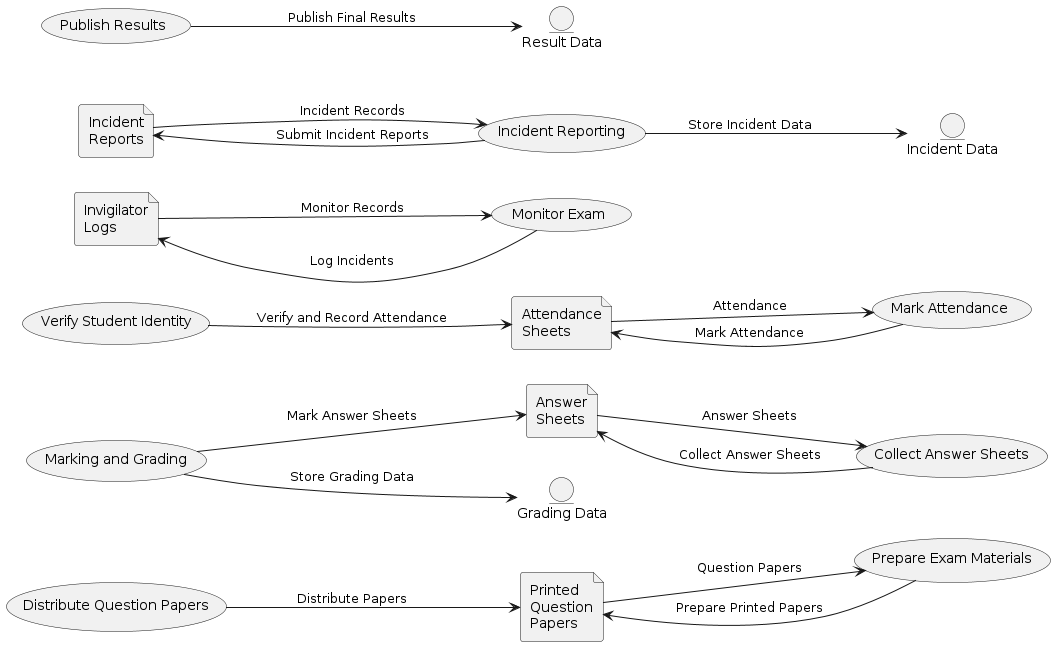
\includegraphics[width=\linewidth]{../figures/dataflow_offline_exam}
	\caption{Dataflow diagram untuk ujian offline.}
	\label{fig:dataflow_offline_exam}
\end{figure}




\subsubsection{Diagram Aliran Data Ujian Offline (Baseline)}

Diagram aliran data untuk sistem ujian offline menunjukkan bagaimana proses ujian dikelola secara manual dengan menggunakan artefak fisik seperti lembar soal, lembar jawaban, dan log pengawas. Berikut adalah penjelasan prosesnya beserta pengkategorian datanya:

\begin{itemize}
	\item \textbf{Dosen} memulai dengan menyiapkan materi ujian, yang kemudian dicetak dan didistribusikan kepada mahasiswa melalui proses "Distribute Question Papers". Hasilnya adalah artefak fisik berupa "Printed Question Papers" (Lembar Soal Cetak).
	\item \textbf{Mahasiswa} memverifikasi identitas mereka, dan kehadiran mereka dicatat dalam "Attendance Sheets" (Lembar Kehadiran) melalui proses "Verify Student Identity" dan "Mark Attendance".
	\item \textbf{Pengawas Ujian} memantau jalannya ujian dan mencatat insiden dalam "Invigilator Logs" (Log Pengawas) melalui proses "Monitor Exam". Jika ada insiden, laporan tersebut dimasukkan dalam "Incident Reports" (Laporan Insiden).
	\item Setelah ujian selesai, lembar jawaban mahasiswa dikumpulkan dalam "Answer Sheets" (Lembar Jawaban) melalui proses "Collect Answer Sheets", yang kemudian digunakan oleh dosen dalam proses penilaian (grading).
	\item \textbf{Dosen} menilai lembar jawaban dan menyimpan hasilnya dalam "Grading Data" (Data Penilaian) melalui proses "Marking and Grading". Setelah penilaian selesai, hasil akhir dipublikasikan melalui proses "Publish Results", yang disimpan dalam "Result Data" (Data Hasil).
	\item Setiap insiden yang dilaporkan selama ujian akan dicatat dalam "Incident Reports" dan datanya disimpan sebagai "Incident Data".
\end{itemize}

\paragraph{Pengkategorian Data Ujian Offline:}
\begin{itemize}
	\item \textbf{Data Fisik:}
	\begin{itemize}
		\item "Printed Question Papers" (Lembar Soal Cetak)
		\item "Answer Sheets" (Lembar Jawaban)
		\item "Attendance Sheets" (Lembar Kehadiran)
		\item "Invigilator Logs" (Log Pengawas)
		\item "Incident Reports" (Laporan Insiden)
	\end{itemize}
	\item \textbf{Data Terstruktur (disimpan dalam database):}
	\begin{itemize}
		\item "Grading Data" (Data Penilaian)
		\item "Result Data" (Data Hasil)
		\item "Incident Data" (Data Insiden)
	\end{itemize}
	\item \textbf{Data Digital Tidak Terstruktur:}
	\begin{itemize}
		\item Tidak relevan untuk sistem ini karena sistem offline mengandalkan artefak fisik.
	\end{itemize}
\end{itemize}

Sistem ini sangat bergantung pada data fisik untuk persiapan dan pengelolaan ujian, sementara hasil penilaian dan data insiden disimpan dalam bentuk data terstruktur yang dapat diakses untuk analisis dan laporan lebih lanjut.

\subsubsection{Diagram Aliran Data Ujian Online (Target)}

\begin{figure}[th!]
	\centering
	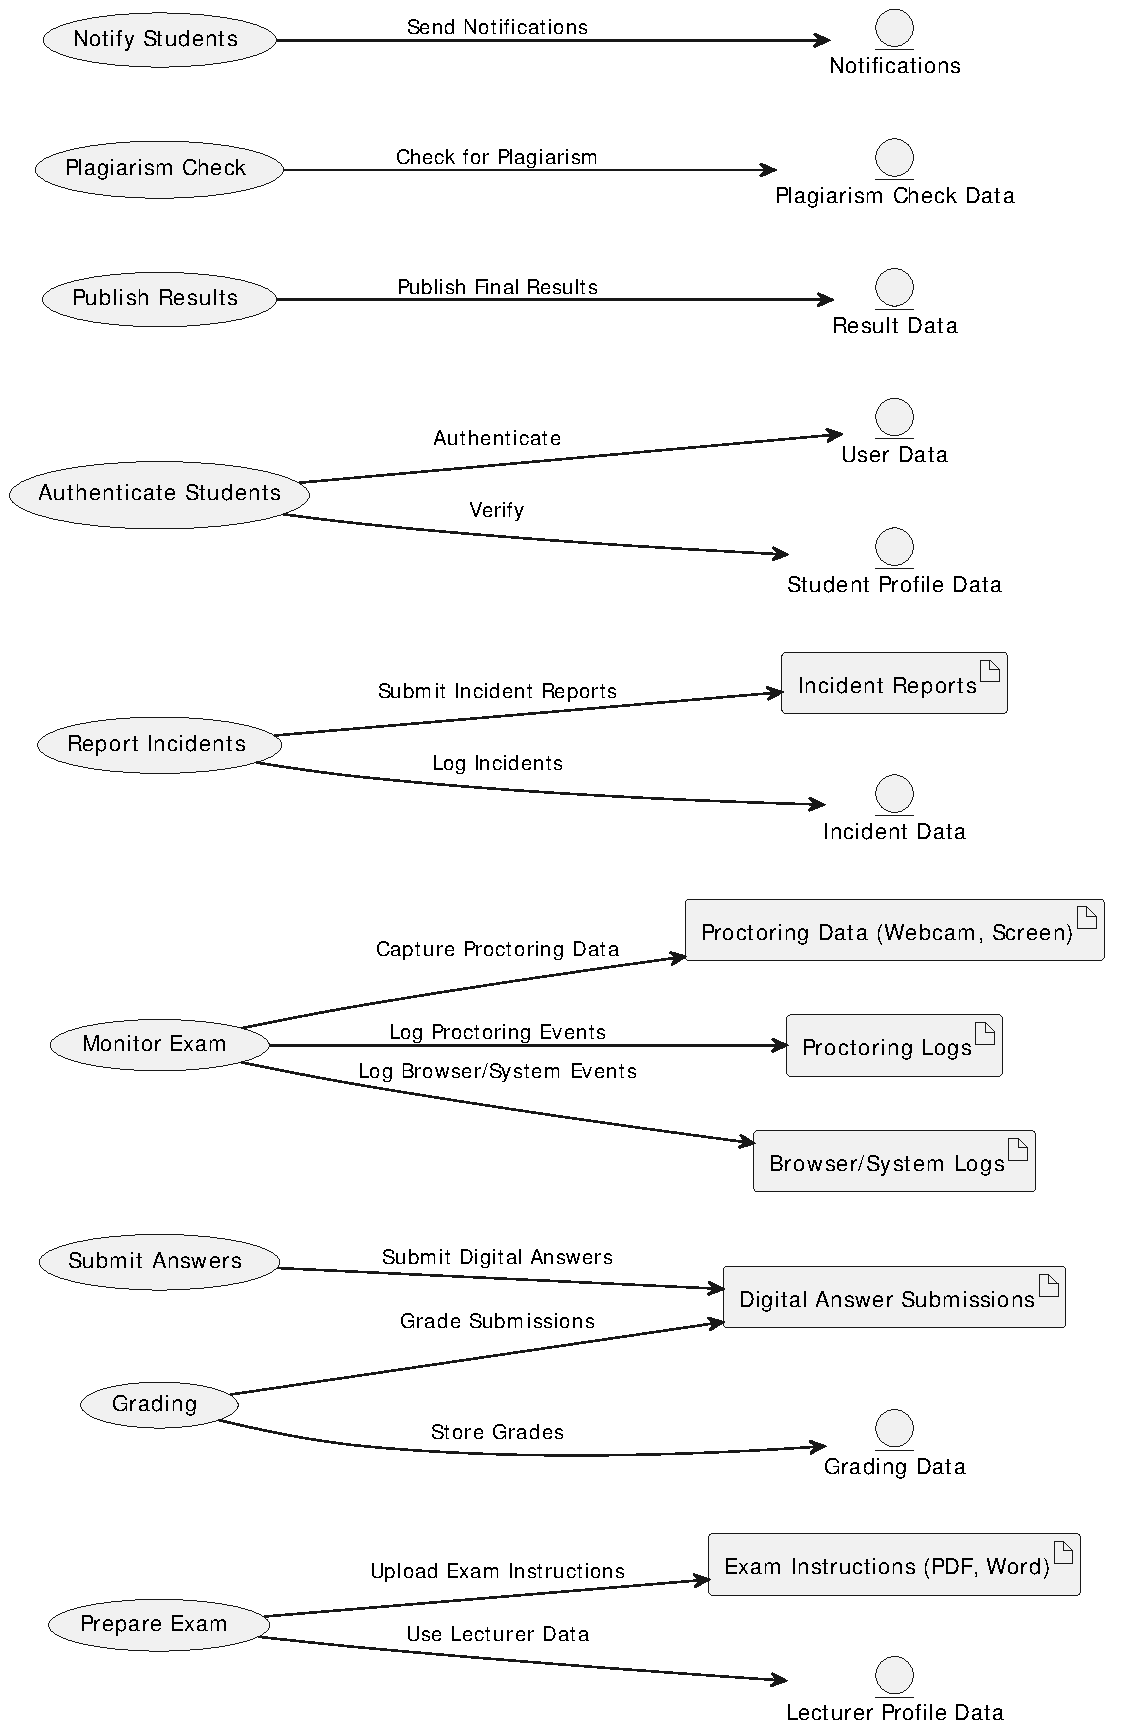
\includegraphics[width=0.7\linewidth]{../figures/dataflow_online_exam}
	\caption{Dataflow diagram untuk ujian online.}
	\label{fig:dataflow_online_exam}
\end{figure}

Diagram aliran data untuk sistem ujian online memperkenalkan otomatisasi dan digitalisasi yang signifikan dalam proses ujian. Berikut adalah penjelasan detailnya, beserta pengkategorian data yang digunakan dalam sistem:

\begin{itemize}
	\item \textbf{Dosen} menyiapkan ujian dengan mengunggah materi ujian, seperti instruksi ujian dalam format PDF atau Word, melalui proses "Prepare Exam". Informasi dosen yang digunakan untuk menyiapkan ujian diambil dari "Lecturer Profile Data".
	\item \textbf{Mahasiswa} harus melakukan autentikasi dan verifikasi identitas melalui proses "Authenticate Students", yang menggunakan data dari "User Data" dan "Student Profile Data".
	\item Selama ujian, \textbf{Platform} memantau aktivitas mahasiswa melalui "Monitor Exam", dengan mengumpulkan data proctoring (misalnya, rekaman webcam atau tangkapan layar) yang disimpan dalam "Proctoring Data", serta mencatat kejadian-kejadian penting dalam "Proctoring Logs". Data dari aktivitas sistem atau browser juga dicatat dalam "Browser/System Logs".
	\item Mahasiswa mengirimkan jawaban ujian secara digital melalui proses "Submit Answers", dan jawaban tersebut disimpan dalam "Digital Answer Submissions".
	\item Setelah pengiriman jawaban, proses "Plagiarism Check" memastikan tidak ada plagiarisme dengan memeriksa data dalam "Plagiarism Check Data". 
	\item \textbf{Dosen} kemudian menilai jawaban mahasiswa melalui proses "Grading", dengan hasil penilaian disimpan dalam "Grading Data". Setelah itu, hasil akhir ujian dipublikasikan melalui "Publish Results" dan disimpan dalam "Result Data".
	\item Mahasiswa menerima pemberitahuan hasil ujian melalui proses "Notify Students", dengan notifikasi yang dikirimkan melalui sistem pemberitahuan dan dicatat dalam "Notifications".
	\item Jika ada insiden selama ujian, laporan insiden tersebut dibuat dalam proses "Report Incidents", dan insiden tersebut dicatat dalam "Incident Reports" serta disimpan sebagai "Incident Data".
\end{itemize}

\paragraph{Pengkategorian Data Ujian Online:}
\begin{itemize}
	\item \textbf{Data Fisik:}
	\begin{itemize}
		\item Tidak ada data fisik, semua proses menggunakan data digital.
	\end{itemize}
	\item \textbf{Data Terstruktur (disimpan dalam database):}
	\begin{itemize}
		\item "User Data" (Data Pengguna)
		\item "Lecturer Profile Data" (Data Profil Dosen)
		\item "Student Profile Data" (Data Profil Mahasiswa)
		\item "Grading Data" (Data Penilaian)
		\item "Result Data" (Data Hasil)
		\item "Incident Data" (Data Insiden)
		\item "Plagiarism Check Data" (Data Pemeriksaan Plagiarisme)
		\item "Notifications" (Pemberitahuan)
	\end{itemize}
	\item \textbf{Data Digital Tidak Terstruktur:}
	\begin{itemize}
		\item "Exam Instructions (PDF, Word)" (Instruksi Ujian)
		\item "Digital Answer Submissions" (Jawaban Digital)
		\item "Proctoring Data (Webcam, Screen)" (Data Proctoring)
		\item "Proctoring Logs" (Log Proctoring)
		\item "Browser/System Logs" (Log Browser/Sistem)
		\item "Incident Reports" (Laporan Insiden)
	\end{itemize}
\end{itemize}

Sistem ujian online bergantung sepenuhnya pada data digital, dengan kombinasi data terstruktur yang disimpan dalam database dan data tidak terstruktur seperti rekaman video, instruksi ujian, dan log sistem yang perlu dikelola secara efisien. Otomatisasi pengelolaan data ini meningkatkan efisiensi, aksesibilitas, dan keamanan dalam mengelola ujian.

Sistem ujian offline bergantung pada penggunaan data fisik, terutama dalam bentuk cetakan dan lembar jawaban, yang memerlukan interaksi manual dan pengelolaan artefak fisik. Sebaliknya, sistem ujian online menggunakan data digital, baik terstruktur maupun tidak terstruktur, yang dikelola secara otomatis oleh platform digital. Sistem online menawarkan efisiensi yang lebih tinggi dan fleksibilitas yang lebih besar dalam manajemen ujian, terutama dalam skenario pembelajaran jarak jauh atau hybrid. Data digital tidak terstruktur seperti rekaman proctoring dan log sistem menjadi elemen penting dalam menjaga integritas dan keamanan ujian online.

\subsection{Analisis Advantages-Disadvantages, Upaya Migrasi, dan Cost-Benefit}

Berdasarkan dataflow diagram untuk ujian offline (baseline) dan online (target), analisis berikut akan membahas kelebihan dan kekurangan dari kedua sistem, langkah-langkah migrasi dari sistem offline ke online, serta analisis biaya-manfaat (cost-benefit) dari transisi ini.

\subsubsection{Analisis Advantages-Disadvantages}

\paragraph{Sistem Ujian Offline (Baseline)}
\textbf{Kelebihan:}
\begin{itemize}
	\item Tidak memerlukan infrastruktur teknologi yang kompleks, sehingga tidak ada ketergantungan pada perangkat digital atau jaringan internet.
	\item Proses sudah dikenal oleh para dosen, pengawas, dan mahasiswa, sehingga tidak memerlukan pelatihan tambahan.
	\item Pengawasan fisik secara langsung (oleh pengawas) dapat lebih mudah mengatasi kecurangan yang jelas terlihat.
\end{itemize}

\textbf{Kekurangan:}
\begin{itemize}
	\item Proses manual memerlukan banyak waktu dan sumber daya (misalnya mencetak soal, mengumpulkan lembar jawaban).
	\item Rentan terhadap kesalahan manusia, baik dalam pencatatan kehadiran, pengumpulan, maupun penilaian.
	\item Pengelolaan insiden (seperti laporan insiden di ruang ujian) memerlukan dokumentasi fisik yang bisa hilang atau rusak.
	\item Skalabilitas terbatas, terutama untuk ujian dengan jumlah mahasiswa yang besar atau pada situasi pembelajaran jarak jauh.
\end{itemize}

\paragraph{Sistem Ujian Online (Target)}
\textbf{Kelebihan:}
\begin{itemize}
	\item Otomatisasi proses seperti pengumpulan jawaban, pengecekan plagiarisme, dan publikasi hasil ujian mengurangi waktu dan sumber daya yang dibutuhkan.
	\item Lebih aman dan efisien dalam pengelolaan data, baik untuk penyimpanan hasil ujian, laporan insiden, maupun pemantauan aktivitas mahasiswa.
	\item Mendukung fleksibilitas bagi mahasiswa yang mengikuti ujian dari jarak jauh atau dalam situasi hybrid.
	\item Data digital seperti log pengawasan dan data proctoring dapat digunakan untuk mengurangi risiko kecurangan dan meningkatkan transparansi.
\end{itemize}

\textbf{Kekurangan:}
\begin{itemize}
	\item Memerlukan infrastruktur teknologi yang handal, termasuk jaringan internet, perangkat keras, dan perangkat lunak yang mendukung.
	\item Risiko keamanan siber, seperti potensi kebocoran data pribadi atau gangguan teknis yang dapat mengganggu proses ujian.
	\item Kurva pembelajaran untuk dosen, mahasiswa, dan pengawas dalam mengoperasikan sistem ujian digital dan pemantauan online.
\end{itemize}

\subsubsection{Upaya Migrasi dari Ujian Offline (Baseline) ke Ujian Online (Target)}

Migrasi dari sistem ujian offline ke sistem ujian online memerlukan beberapa upaya yang meliputi:

\begin{enumerate}
	\item \textbf{Penyiapan Infrastruktur Teknologi:}
	\begin{itemize}
		\item Pengadaan platform ujian online, perangkat keras, dan jaringan yang mendukung kelancaran ujian online.
		\item Menyiapkan ruang server dan penyimpanan untuk menangani data digital besar seperti rekaman proctoring, log sistem, dan hasil ujian.
	\end{itemize}
	\item \textbf{Pelatihan dan Familiarisasi:}
	\begin{itemize}
		\item Melatih dosen, mahasiswa, dan pengawas dalam penggunaan platform ujian, termasuk cara menggunakan proctoring dan pengecekan plagiarisme.
		\item Menyediakan panduan dan simulasi ujian online untuk memastikan semua pihak terbiasa dengan sistem baru.
	\end{itemize}
	\item \textbf{Keamanan dan Kebijakan Penggunaan:}
	\begin{itemize}
		\item Mengembangkan kebijakan keamanan data dan protokol dalam menangani masalah teknis serta potensi kecurangan digital.
		\item Menerapkan prosedur yang jelas untuk menangani insiden yang terkait dengan pemantauan dan proctoring secara online.
	\end{itemize}
	\item \textbf{Uji Coba dan Pengawasan:}
	\begin{itemize}
		\item Melakukan uji coba sistem ujian online dengan kelompok kecil untuk memastikan bahwa sistem berjalan dengan baik tanpa masalah teknis.
		\item Menerapkan sistem pemantauan dan audit terhadap proses ujian online untuk memastikan integritas dan keamanan ujian.
	\end{itemize}
\end{enumerate}

\subsubsection{Analisis Cost-Benefit}

\paragraph{Biaya:}
\begin{itemize}
	\item \textbf{Pengadaan Teknologi:} Pengeluaran awal yang signifikan untuk pengadaan platform ujian online, perangkat keras tambahan, server, serta perangkat proctoring.
	\item \textbf{Pelatihan:} Biaya untuk pelatihan staf pengajar, pengawas, dan mahasiswa dalam penggunaan sistem baru, serta pembuatan materi panduan.
	\item \textbf{Pemeliharaan dan Dukungan Teknis:} Biaya berkelanjutan untuk pemeliharaan sistem, dukungan teknis, serta pembaruan perangkat lunak dan keamanan.
	\item \textbf{Keamanan dan Perlindungan Data:} Pengeluaran tambahan untuk memastikan keamanan data mahasiswa dan mencegah potensi ancaman siber.
\end{itemize}

\paragraph{Manfaat:}
\begin{itemize}
	\item \textbf{Efisiensi Waktu dan Biaya Operasional:} Otomatisasi proses pengumpulan, penilaian, dan publikasi hasil ujian mengurangi beban kerja manual dan waktu pemrosesan.
	\item \textbf{Aksesibilitas dan Skalabilitas:} Mahasiswa dapat mengikuti ujian dari lokasi mana pun, sehingga mendukung pembelajaran jarak jauh dan hybrid. Sistem ini juga mampu menangani jumlah mahasiswa yang lebih besar secara efisien.
	\item \textbf{Pengelolaan Data yang Lebih Baik:} Penyimpanan digital memudahkan pengelolaan data secara terpusat dan memastikan transparansi hasil ujian serta catatan insiden.
	\item \textbf{Peningkatan Keamanan Ujian:} Penggunaan proctoring digital, log aktivitas, dan pengecekan plagiarisme meningkatkan integritas dan keadilan dalam pelaksanaan ujian.
\end{itemize}

Walaupun terdapat biaya awal yang cukup besar dalam implementasi sistem ujian online, manfaat jangka panjang seperti efisiensi, aksesibilitas, dan peningkatan keamanan menjadikannya solusi yang sangat bermanfaat. Selain itu, sistem online memungkinkan pengelolaan ujian secara lebih fleksibel dan terstruktur, terutama dalam skenario pembelajaran jarak jauh.


\section{Aktivitas Kelas dan Tugas}
Buat model data dan dokumen \textbf{As-Is} yang terpengaruh oleh kapabilitas yang dipilih. Selain itu, buat model data dan dokumen \textbf{To-Be} yang diperlukan untuk mewujudkan kapbilitas terpilih. Tuangkan dalam bentuk atau perbaharui Dokumen Definisi Arsitektur (Subbab \ref{sec:isi_dokumen_definisi_arsitektur} dan \ref{sec:dokumen_definisi_arsitektur_data}) dan Spesifikasi Persyaratan Arsitektur (Subbab \ref{sec:spesifikasi_kebutuhan_arsitektur} dan  \ref{sec:spesifikasi_kebutuhan_arsitektur_data}).

	\chapter{Arsitektur Aplikasi}

\section{Tujuan}
Mengembangkan arsitektur aplikasi target yang mendukung bisnis sangat penting untuk menyelaraskan strategi bisnis dengan kapabilitas teknologi. Ini mencakup pembuatan visi arsitektur sekaligus menangani permintaan pekerjaan arsitektur dan kepentingan pemangku kepentingan. Selain itu, identifikasi komponen kandidat untuk peta jalan arsitektur membantu mengatasi kesenjangan antara arsitektur aplikasi saat ini dan yang diinginkan.

\section{Input untuk Pengembangan Arsitektur Aplikasi}

\subsection{Permintaan Pekerjaan Arsitektur}
Input yang digunakan dalam fase ini meliputi:

\begin{enumerate}
	\item Penilaian Kapabilitas
	\item Rencana Komunikasi
	\item Model Organisasi untuk Arsitektur Perusahaan
	\item Kerangka Kerja Arsitektur yang Disesuaikan
	\item Spesifikasi Kebutuhan Arsitektur Awal, termasuk:
	\begin{enumerate}
		\item Hasil Analisis Kesenjangan
		\item Persyaratan teknis lainnya yang relevan
	\end{enumerate}
	\item Dokumen definisi arsitektur (draf)
	\begin{enumerate}
		
	\item Arsitektur Bisnis Saat Ini (rinci)
	\item Arsitektur Bisnis Target (rinci)
	\item Arsitektur Data Saat Ini (rinci)
	\item Arsitektur Data Target (rinci)
	\item Arsitektur Aplikasi Saat Ini (garis besar)
	\item Arsitektur Aplikasi Target (garis besar)
	\item Arsitektur Teknologi Saat Ini (garis besar)
	\item Arsitektur Teknologi Target (garis besar)
\end{enumerate}

	\item Prinsip Aplikasi, jika ada
	\item Pernyataan Pekerjaan Arsitektur
	\item Visi Arsitektur
	\item Repositori Arsitektur
	\item Komponen Arsitektur Bisnis dalam Peta Jalan Arsitektur
\end{enumerate}

\section{Prinsip Aplikasi}
\begin{itemize}
	\item \textbf{Independensi Teknologi}.
	Aplikasi tidak tergantung pada pilihan teknologi tertentu, sehingga memberikan fleksibilitas untuk beroperasi di berbagai platform teknologi.
	
	\item \textbf{Kemudahan Penggunaan}.
	Aplikasi harus mudah digunakan. Teknologi yang mendasari harus transparan bagi pengguna, sehingga mereka dapat fokus pada penyelesaian tugas dengan efektif.
\end{itemize}

\section{Langkah-langkah dalam Pengembangan Arsitektur Aplikasi}
Langkah-langkah berikut sangat penting dalam pengembangan arsitektur aplikasi yang kokoh:

\begin{enumerate}
	\item Pilih model referensi, sudut pandang, dan alat yang sesuai
	\item Mengembangkan Deskripsi Arsitektur Aplikasi Saat Ini
	\item Mengembangkan Deskripsi Arsitektur Aplikasi Target
	\item Melakukan Analisis Kesenjangan
	\item Menentukan komponen peta jalan kandidat
	\item Menyelesaikan dampak di seluruh Lanskap Arsitektur
	\item Melakukan Analisis Pemangku Kepentingan Formal
	\item Menyelesaikan Arsitektur Aplikasi
	\item Membuat Dokumen Definisi Arsitektur
\end{enumerate}

\subsection*{Contoh:}
\begin{enumerate}
	\item \textbf{Pilih model referensi, sudut pandang, dan alat yang sesuai}: Langkah pertama dalam proses pengembangan arsitektur aplikasi adalah memilih model referensi yang relevan (misalnya TOGAF, Zachman), sudut pandang yang akan digunakan (misalnya sudut pandang pemangku kepentingan, sudut pandang implementasi teknis), serta alat bantu yang mendukung (misalnya ArchiMate, Enterprise Architect). Pemilihan ini akan memengaruhi cara arsitektur didefinisikan dan dikomunikasikan.
	\\
	\textit{Contoh:} Universitas menggunakan model referensi TOGAF untuk mendefinisikan dan mengelola arsitektur teknologi, memilih sudut pandang pemangku kepentingan (mahasiswa, dosen, admin) untuk memastikan bahwa setiap kebutuhan dipenuhi.
	
	\item \textbf{Mengembangkan Deskripsi Arsitektur Aplikasi Saat Ini}: Deskripsi ini mendokumentasikan keadaan saat ini dari arsitektur aplikasi, termasuk aplikasi yang digunakan, fungsionalitas, dan interaksi antar aplikasi. Deskripsi ini penting untuk memahami baseline sebelum merencanakan perubahan.
	\\
	\textit{Contoh:} Universitas memiliki deskripsi arsitektur aplikasi saat ini yang mencakup LMS, sistem keuangan, dan sistem pendaftaran online, serta bagaimana aplikasi tersebut saling terhubung.
	
	\item \textbf{Mengembangkan Deskripsi Arsitektur Aplikasi Target}: Deskripsi ini berfokus pada arsitektur aplikasi yang diinginkan di masa mendatang, mencakup aplikasi baru yang akan diimplementasikan, fitur tambahan, atau integrasi yang lebih baik antara sistem. Hal ini membantu mengarahkan langkah-langkah perbaikan ke arah yang tepat.
	\\
	\textit{Contoh:} Arsitektur aplikasi target universitas mencakup integrasi penuh antara sistem LMS dan sistem manajemen kursus, serta penambahan platform kolaborasi daring untuk mendukung pembelajaran hybrid.
	
	\item \textbf{Melakukan Analisis Kesenjangan}: Analisis ini membandingkan arsitektur aplikasi saat ini dengan arsitektur target untuk mengidentifikasi kesenjangan dan menentukan langkah-langkah yang perlu dilakukan untuk menjembataninya.
	\\
	\textit{Contoh:} Analisis kesenjangan menunjukkan bahwa universitas saat ini tidak memiliki fitur penjadwalan otomatis pada LMS yang diinginkan pada arsitektur aplikasi target untuk mendukung pembelajaran hybrid.
	
	\item \textbf{Menentukan komponen peta jalan kandidat}: Setelah analisis kesenjangan dilakukan, langkah berikutnya adalah menentukan komponen-komponen yang harus dimasukkan ke dalam peta jalan (roadmap) untuk mencapai arsitektur target. Ini termasuk penentuan prioritas, waktu pelaksanaan, dan sumber daya yang diperlukan.
	\\
	\textit{Contoh:} Universitas memprioritaskan integrasi LMS dengan sistem manajemen kursus sebagai komponen utama peta jalan mereka, yang dijadwalkan selesai dalam dua semester.
	
	\item \textbf{Menyelesaikan dampak di seluruh Lanskap Arsitektur}: Setiap perubahan pada arsitektur aplikasi dapat berdampak pada arsitektur lain, seperti arsitektur data, arsitektur teknologi, atau bahkan arsitektur bisnis. Langkah ini memastikan bahwa dampak tersebut diidentifikasi dan dikelola dengan tepat.
	\\
	\textit{Contoh:} Integrasi LMS dengan sistem manajemen kursus dipastikan tidak mengganggu arsitektur data mahasiswa, dengan mengelola akses yang aman antara dua sistem tersebut.
	
	\item \textbf{Melakukan Analisis Pemangku Kepentingan Formal}: Pada tahap ini, kebutuhan dan kepentingan pemangku kepentingan, seperti mahasiswa, dosen, dan admin, dianalisis secara formal untuk memastikan bahwa arsitektur aplikasi memenuhi kebutuhan mereka.
	\\
	\textit{Contoh:} Universitas melakukan survei kepada mahasiswa dan dosen untuk memastikan bahwa perubahan pada LMS memenuhi kebutuhan mereka akan kemudahan akses dan efisiensi.
	
	\item \textbf{Menyelesaikan Arsitektur Aplikasi}: Setelah seluruh komponen di atas selesai dianalisis, arsitektur aplikasi diselesaikan. Ini melibatkan finalisasi rancangan, pengaturan sumber daya, dan perencanaan implementasi.
	\\
	\textit{Contoh:} Universitas telah menyelesaikan arsitektur aplikasi dengan mengintegrasikan semua sistem yang mendukung pembelajaran hybrid secara efisien.
	
	\item \textbf{Membuat Dokumen Definisi Arsitektur}: Langkah terakhir adalah mendokumentasikan seluruh arsitektur dalam dokumen formal. Dokumen ini mencakup semua aspek yang telah direncanakan, termasuk deskripsi aplikasi saat ini dan target, analisis kesenjangan, peta jalan, dan strategi implementasi.
	\\
	\textit{Contoh:} Universitas menyusun Dokumen Definisi Arsitektur yang mencakup semua aplikasi yang akan diintegrasikan, roadmap untuk perubahan, dan rencana pemantauan dampak bagi pengguna.
\end{enumerate}

\section{Hasil (\textit{Output}) dari Pengembangan Arsitektur Aplikasi}
Hasil dari fase ini memastikan pengembangan dan validasi arsitektur aplikasi yang mendukung arsitektur bisnis. Hasil tersebut meliputi:

\begin{enumerate}
	\item Pernyataan Pekerjaan Arsitektur, diperbarui sesuai kebutuhan
	\item Prinsip aplikasi yang divalidasi atau prinsip aplikasi baru
	\item Dokumen Definisi Arsitektur, diperbarui sesuai kebutuhan
	\item Spesifikasi Kebutuhan Arsitektur , diperbarui sesuai kebutuhan
	\item Komponen Arsitektur Aplikasi dalam Peta Jalan Arsitektur
\end{enumerate}

\section{Katalog, Matriks, dan Diagram Arsitektur Aplikasi}
Alat dan representasi berikut digunakan untuk mendokumentasikan dan menganalisis arsitektur aplikasi:

\begin{itemize}
\item Katalog
\begin{itemize}
	\item Katalog Portofolio Aplikasi
	\item Katalog Antarmuka
\end{itemize}

\item Matriks
\begin{itemize}
	\item Matriks Aplikasi/Organisasi
	\item Matriks Peran/Aplikasi
	\item Matriks Aplikasi/Fungsi
	\item Matriks Interaksi Aplikasi
\end{itemize}

\item Diagram
\begin{itemize}
	\item Diagram Komunikasi Aplikasi
	\item Diagram Lokasi Aplikasi dan Pengguna
	\item Diagram Use-Case Aplikasi
	\item Diagram Kemudahan Manajemen Perusahaan
	\item Diagram Realisasi Proses/Aplikasi
	\item Diagram Rekayasa Perangkat Lunak
	\item Diagram Migrasi Aplikasi
	\item Diagram Distribusi Perangkat Lunak
\end{itemize}

\end{itemize}


\subsection*{Contoh:}

\begin{itemize}
	\item \textbf{Katalog}: Katalog berisi daftar terstruktur dari berbagai elemen terkait aplikasi dan antarmuka yang digunakan dalam arsitektur aplikasi.
	
	\begin{itemize}
		\item \textbf{Katalog Portofolio Aplikasi}: Berisi daftar semua aplikasi yang digunakan dalam suatu organisasi. Katalog ini mencakup informasi tentang fungsi aplikasi, statusnya (aktif, dalam pengembangan, atau dihentikan), dan bagaimana aplikasi tersebut mendukung proses bisnis organisasi. \\
		\textit{Contoh:} Katalog aplikasi di universitas yang mencakup Learning Management System (LMS), sistem informasi akademik, dan aplikasi administrasi keuangan.
		
		\item \textbf{Katalog Antarmuka}: Berisi daftar antarmuka yang menghubungkan berbagai aplikasi dalam sistem. Katalog ini menjelaskan bagaimana data ditransfer antar aplikasi, termasuk protokol komunikasi dan format data yang digunakan. \\
		\textit{Contoh:} Katalog antarmuka antara sistem LMS dan sistem manajemen sumber daya manusia (HRMS) di universitas untuk menyinkronkan data kehadiran dosen dan mahasiswa.
	\end{itemize}
	
	\item \textbf{Matriks}: Matriks menggambarkan hubungan antara berbagai elemen seperti aplikasi, peran, fungsi, dan interaksi dalam arsitektur aplikasi.
	
	\begin{itemize}
		\item \textbf{Matriks Aplikasi/Organisasi}: Menunjukkan hubungan antara aplikasi yang digunakan dan unit organisasi yang bertanggung jawab atas aplikasi tersebut. Matriks ini membantu mengidentifikasi tanggung jawab dan pengelolaan aplikasi di berbagai departemen. \\
		\textit{Contoh:} Matriks yang menunjukkan bahwa departemen IT bertanggung jawab atas manajemen LMS, sedangkan departemen keuangan bertanggung jawab atas aplikasi penggajian.
		
		\item \textbf{Matriks Peran/Aplikasi}: Menggambarkan hubungan antara peran pengguna (misalnya, dosen, mahasiswa, staf administrasi) dan aplikasi yang digunakan oleh masing-masing peran. Matriks ini memastikan setiap peran memiliki akses ke aplikasi yang tepat. \\
		\textit{Contoh:} Matriks yang menunjukkan bahwa dosen memiliki akses ke sistem evaluasi akademik, sementara mahasiswa memiliki akses ke sistem pengelolaan tugas di LMS.
		
		\item \textbf{Matriks Aplikasi/Fungsi}: Menggambarkan hubungan antara aplikasi dan fungsi bisnis yang mereka dukung. Matriks ini menunjukkan bagaimana aplikasi mendukung berbagai aktivitas bisnis. \\
		\textit{Contoh:} Matriks yang menunjukkan bahwa aplikasi ERP mendukung fungsi keuangan, pengadaan, dan manajemen inventaris.
		
		\item \textbf{Matriks Interaksi Aplikasi}: Menggambarkan interaksi antara aplikasi yang berbeda dalam suatu sistem, membantu memahami bagaimana data dan proses bergerak di antara aplikasi. \\
		\textit{Contoh:} Matriks yang menunjukkan interaksi antara sistem manajemen data mahasiswa dan sistem LMS dalam pembaruan status akademik secara otomatis.
	\end{itemize}
	
	\item \textbf{Diagram}: Diagram memberikan representasi visual dari berbagai aspek arsitektur aplikasi, seperti komunikasi, interaksi, dan distribusi.
	
	\begin{itemize}
		\item \textbf{Diagram Komunikasi Aplikasi}: Menggambarkan bagaimana aplikasi berkomunikasi satu sama lain, baik melalui antarmuka, API, atau protokol jaringan lainnya. \\
		\textit{Contoh:} Diagram yang menunjukkan komunikasi antara sistem pendaftaran online dengan sistem pembayaran universitas.
		
		\item \textbf{Diagram Lokasi Aplikasi dan Pengguna}: Menunjukkan lokasi fisik dan geografis dari aplikasi serta pengguna yang mengakses aplikasi tersebut. Diagram ini penting dalam konteks distribusi geografis, terutama untuk organisasi yang memiliki banyak lokasi. \\
		\textit{Contoh:} Diagram yang menunjukkan akses aplikasi LMS oleh mahasiswa dari berbagai lokasi, baik di kampus maupun dari rumah.
		
		\item \textbf{Diagram Use-Case Aplikasi}: Menggambarkan berbagai skenario penggunaan aplikasi oleh pengguna dalam konteks tertentu. Ini membantu memahami bagaimana aplikasi memenuhi kebutuhan pengguna. \\
		\textit{Contoh:} Diagram use-case yang menunjukkan bagaimana mahasiswa menggunakan LMS untuk mengunduh tugas, mengikuti ujian daring, dan mengakses materi kuliah.
		
		\item \textbf{Diagram Kemudahan Manajemen Perusahaan}: Menunjukkan bagaimana aplikasi mendukung manajemen operasional dan strategis perusahaan, termasuk integrasi antara aplikasi yang berbeda dalam mendukung proses pengambilan keputusan. \\
		\textit{Contoh:} Diagram yang menunjukkan bagaimana data keuangan dari sistem ERP digunakan oleh manajemen untuk perencanaan anggaran.
		
		\item \textbf{Diagram Realisasi Proses/Aplikasi}: Menggambarkan bagaimana aplikasi mendukung realisasi proses bisnis, seperti alur kerja, otomatisasi tugas, dan integrasi proses lintas aplikasi. \\
		\textit{Contoh:} Diagram yang menunjukkan bagaimana aplikasi manajemen proyek terintegrasi dengan sistem waktu kerja dan pelaporan kinerja di universitas.
		
		\item \textbf{Diagram Rekayasa Perangkat Lunak}: Menunjukkan struktur perangkat lunak, modul-modul utama, dan hubungan antar modul dalam pengembangan aplikasi. \\
		\textit{Contoh:} Diagram yang menunjukkan modul utama dalam sistem manajemen kursus daring, termasuk modul manajemen konten, modul diskusi, dan modul penilaian.
		
		\item \textbf{Diagram Migrasi Aplikasi}: Menggambarkan proses migrasi dari satu sistem aplikasi ke sistem yang lain, termasuk tahapan, data yang dipindahkan, dan integrasi dengan sistem lain selama proses migrasi. \\
		\textit{Contoh:} Diagram yang menunjukkan migrasi data dari sistem LMS lama ke platform e-learning baru di universitas.
		
		\item \textbf{Diagram Distribusi Perangkat Lunak}: Menunjukkan bagaimana perangkat lunak didistribusikan ke berbagai pengguna atau sistem dalam organisasi. Ini mencakup jalur distribusi dan mekanisme pembaruan perangkat lunak. \\
		\textit{Contoh:} Diagram distribusi yang menunjukkan bagaimana pembaruan perangkat lunak LMS dikirimkan ke berbagai server yang mengelola akses mahasiswa dan dosen.
	\end{itemize}
\end{itemize}

\section{Dokumen Definisi Arsitektur dengan Penambahan Arsitektur Aplikasi}
\label{sec:dokumen_definisi_arsitektur_aplikasi}

Topik-topik yang perlu dibahas dalam Architecture Definition Document yang terkait dengan Application Architecture dalam konteks pembelajaran dan pengajaran hybrid di universitas adalah sebagai berikut:

\begin{itemize}
	\item Baseline Application Architecture, jika sesuai
	\item Target Application Architecture
	\item Tampilan Arsitektur Aplikasi yang sesuai dengan sudut pandang yang dipilih, yang mengatasi kekhawatiran utama pemangku kepentingan
\end{itemize}

\subsection*{Contoh:}

Berikut adalah beberapa contoh arsitektur aplikasi dalam konteks pembelajaran hybrid di universitas:

\begin{itemize}
	\item \textbf{Baseline Application Architecture:} Universitas menggunakan sistem Learning Management System (LMS) seperti Moodle atau Google Classroom untuk mendukung pembelajaran daring, dan platform konferensi video seperti Zoom atau Microsoft Teams untuk kuliah daring. 
	
	\item \textbf{Target Application Architecture:} Sistem yang dirancang untuk meningkatkan integrasi antara pembelajaran daring dan tatap muka, serta mendukung interaksi yang lebih baik bagi mahasiswa dan dosen dalam konteks hybrid. 
	
	\begin{itemize}
		\item \textbf{Model Sistem Proses:} Sebuah sistem hybrid yang mendukung proses pengajaran di mana kuliah dapat direkam dan disiarkan langsung secara bersamaan. Mahasiswa dapat berinteraksi dengan dosen secara real-time, dan rekaman kuliah otomatis disimpan di LMS untuk akses asinkron.
		\item \textbf{Model Sistem Tempat:} Sistem ini memungkinkan dosen untuk mengajar dari ruang kelas yang dilengkapi teknologi hybrid, sementara mahasiswa dapat bergabung dari rumah atau lokasi lain melalui perangkat mereka.
		\item \textbf{Model Sistem Waktu:} LMS yang mendukung penjadwalan otomatis untuk kuliah sinkron dan pengelolaan tugas yang dapat diakses asinkron oleh mahasiswa, sehingga fleksibel dengan waktu belajar yang berbeda.
		\item \textbf{Model Sistem Orang:} Portal yang mendukung interaksi antara dosen dan mahasiswa, di mana dosen dapat memberikan umpan balik langsung secara daring, dan mahasiswa dapat berkolaborasi dalam proyek kelompok.
	\end{itemize}
	
	\item \textbf{Tampilan Arsitektur Aplikasi:} Tampilan yang menunjukkan integrasi aplikasi pembelajaran hybrid. Ini bisa mencakup integrasi antara platform video conferencing seperti Zoom dengan LMS, sehingga rekaman kuliah dapat diakses oleh mahasiswa setelah sesi berakhir.
	
	\begin{itemize}
		\item Tampilan arsitektur ini juga mencakup bagaimana platform tersebut mendukung dosen dalam penjadwalan kelas secara otomatis, serta bagaimana sistem mendukung evaluasi dan umpan balik secara digital.
	\end{itemize}
\end{itemize}

\section{Spesifikasi Kebutuhan Arsitektur dengan Penambahan Arsitektur Aplikasi}
\label{sec:spesifikasi_kebutuhan_arsitektur_aplikasi}

Kebutuhan Arsitektur Aplikasi yang mengisi Spesifikasi Kebutuhan Arsitektur pada Fase C meliputi:

\begin{itemize}
	\item Hasil Analisis Kesenjangan
	\item Kebutuhan interoperabilitas aplikasi
	\item Kebutuhan teknis yang relevan yang akan berlaku untuk evolusi ini dari Siklus Pengembangan Arsitektur
	\item Kendala pada Arsitektur Teknologi yang akan dirancang
	\item Kebutuhan bisnis yang diperbarui, jika sesuai
	\item Kebutuhan data yang diperbarui, jika sesuai
\end{itemize}

\subsection*{Contoh:}

Berikut adalah beberapa contoh kebutuhan arsitektur aplikasi dalam konteks pembelajaran hybrid di universitas:

\begin{itemize}
	\item \textbf{Hasil Analisis Kesenjangan:} Dalam penerapan sistem hybrid di universitas, hasil analisis kesenjangan menunjukkan bahwa beberapa platform e-learning yang ada tidak dapat diintegrasikan dengan baik dengan sistem manajemen penjadwalan universitas. Hal ini menciptakan kesenjangan dalam penyelarasan proses antara kelas daring dan kelas tatap muka.
	
	\item \textbf{Kebutuhan Interoperabilitas Aplikasi:} Dalam pengembangan lebih lanjut, aplikasi hybrid harus memiliki kemampuan untuk berinteroperasi antara berbagai sistem, seperti LMS, sistem konferensi video, dan sistem manajemen universitas, sehingga data dari berbagai platform dapat diakses dan dikelola secara terintegrasi.
	
	\item \textbf{Kebutuhan Teknis:} Untuk memastikan kelancaran pembelajaran hybrid, diperlukan kebutuhan teknis yang relevan, seperti ketersediaan bandwidth untuk mendukung streaming video langsung, serta integrasi yang mulus antara perangkat keras di ruang kelas (misalnya, kamera dan mikrofon) dengan perangkat lunak.
	
	\item \textbf{Kendala pada Arsitektur Teknologi:} Teknologi saat ini yang digunakan untuk kelas tatap muka mungkin tidak mendukung semua aspek pembelajaran hybrid, seperti kemampuan untuk merekam sesi dan streaming secara simultan, yang menjadi kendala dalam perancangan arsitektur teknologi baru.
	
	\item \textbf{Kebutuhan Bisnis yang Diperbarui:} Kebutuhan bisnis untuk sistem hybrid meliputi peningkatan aksesibilitas dan inklusivitas bagi mahasiswa yang tidak dapat hadir secara fisik, sehingga solusi arsitektur aplikasi harus mencakup akses ke materi kuliah secara daring.
	
	\item \textbf{Kebutuhan Data yang Diperbarui:} Dalam konteks hybrid, diperlukan kebutuhan data yang diperbarui, termasuk cara mengelola data mahasiswa dan pelacakan kehadiran yang dilakukan secara daring maupun luring, serta memastikan bahwa data privasi mahasiswa dilindungi dengan baik.
\end{itemize}


\section{Beberapa Pertimbangan untuk Kasus Kerja Jarak Jauh}
Dengan meningkatnya kerja jarak jauh, perhatian khusus perlu diberikan pada beberapa aspek terkait aplikasi:

\begin{enumerate}
	\item Migrasi ke aplikasi untuk kolaborasi kerja daring
	\item Perubahan proses bisnis, yang mungkin menyebabkan perubahan aplikasi
	\item Keamanan aplikasi: enkripsi, manajemen kata sandi, hak akses, dll.
	\item Tata kelola aplikasi: siapa yang bertanggung jawab atas aplikasi atau tugas terkait aplikasi
	\item Manajemen aplikasi: manajemen pemecahan masalah, dukungan pengguna, dukungan dari vendor, perizinan, dan pembaruan
	\item Biaya aplikasi: keuangan, perizinan, kinerja, dan fitur
\end{enumerate}

\section{Aplikasi Terkait Perusahaan}
Aplikasi terkait perusahaan membentuk tulang punggung bisnis modern. Beberapa jenis aplikasi perusahaan meliputi:

\begin{enumerate}
	\item \textbf{Enterprise Resource Planning (ERP)}: Sistem yang mengintegrasikan berbagai fungsi bisnis utama, seperti akuntansi, sumber daya manusia, penjualan, dan produksi, ke dalam satu sistem yang terpusat. Contoh: SAP ERP, Oracle ERP, Microsoft Dynamics 365, Odoo.
	
	\item \textbf{Customer Relationship Management (CRM)}: Sistem yang digunakan untuk mengelola interaksi perusahaan dengan pelanggan dan calon pelanggan, membantu meningkatkan hubungan dan kepuasan pelanggan. Contoh: Salesforce, HubSpot CRM, Zoho CRM, Microsoft Dynamics CRM.
	
	\item \textbf{Supply Chain Management (SCM)}: Sistem yang membantu mengelola aliran barang, informasi, dan uang di sepanjang rantai pasokan, mulai dari pemasok hingga pelanggan akhir. Contoh: SAP SCM, Oracle SCM Cloud, Kinaxis, Infor Supply Chain Management.
	
	\item \textbf{Business Intelligence}: Teknologi dan strategi yang digunakan oleh perusahaan untuk menganalisis data bisnis, menghasilkan wawasan yang dapat digunakan untuk pengambilan keputusan. Contoh: Power BI, Tableau, Qlik Sense, SAP BusinessObjects.
	
	\item \textbf{Point of Sales (PoS)}: Sistem yang digunakan untuk melakukan transaksi penjualan di lokasi fisik atau online, sering kali mencakup pemrosesan pembayaran, pelacakan inventaris, dan laporan penjualan. Contoh: Square, Shopify POS, Toast POS, Lightspeed POS.
	
	\item \textbf{Manufacturing Execution System (MES)}: Sistem yang digunakan untuk melacak dan mengelola produksi di pabrik, membantu dalam perencanaan produksi, pengawasan, dan pengoptimalan proses manufaktur. Contoh: Siemens Opcenter, Rockwell Automation FactoryTalk, Dassault Systèmes DELMIA, Honeywell MES.
	
	\item \textbf{Human Resource Management System (HRMS)}: Sistem yang membantu mengelola proses sumber daya manusia seperti penggajian, rekrutmen, pelatihan, dan pengelolaan kinerja karyawan. Contoh: Workday, SAP SuccessFactors, BambooHR, ADP Workforce Now.
	
	\item \textbf{Maintenance Management System (MMS)}: Sistem yang digunakan untuk merencanakan, melacak, dan mengelola pemeliharaan aset perusahaan, baik untuk perawatan preventif maupun reaktif. Contoh: IBM Maximo, Fiix, UpKeep, Limble CMMS.
	
	\item \textbf{Warehouse Management System (WMS)}: Sistem yang digunakan untuk mengelola operasi gudang, seperti pelacakan inventaris, manajemen lokasi penyimpanan, dan pemrosesan pengiriman. Contoh: Manhattan Associates WMS, SAP Extended Warehouse Management, Oracle WMS, Infor CloudSuite WMS.
	
	\item \textbf{Manufacturing Intelligence (MI)}: Sistem yang mengumpulkan dan menganalisis data dari proses manufaktur untuk meningkatkan kinerja operasional dan kualitas produk. Contoh: GE Digital Proficy, Siemens MindSphere, Honeywell Process Solutions, Rockwell Automation FactoryTalk Analytics.
	
	\item \textbf{Quality Management System (QMS)}: Sistem yang membantu organisasi dalam memastikan bahwa produk atau layanan yang mereka hasilkan memenuhi standar kualitas yang ditetapkan. Contoh: MasterControl, Arena QMS, ETQ Reliance, Sparta Systems TrackWise.
	
	\item \textbf{Knowledge Management System (KMS)}: Sistem yang digunakan untuk menangkap, menyimpan, dan berbagi pengetahuan dalam organisasi, sering kali melibatkan kolaborasi dan akses informasi yang mudah. Contoh: Confluence, Microsoft SharePoint, Notion, Zendesk Knowledge Management.
	
	\item \textbf{Transportation Management System (TMS)}: Sistem yang digunakan untuk merencanakan, melaksanakan, dan mengoptimalkan pengiriman barang, termasuk pengelolaan logistik dan pengangkutan. Contoh: SAP Transportation Management, Oracle Transportation Management, JDA TMS, Manhattan TMS.
	
	\item \textbf{Fleet Management System (FMS)}: Sistem yang digunakan untuk melacak dan mengelola armada kendaraan perusahaan, termasuk pemeliharaan, rute, dan pemantauan pengemudi. Contoh: Samsara, Geotab, Verizon Connect, Fleet Complete.
\end{enumerate}



\section{Ringkasan}
Fase Arsitektur Aplikasi sangat penting untuk mendefinisikan dan memvalidasi arsitektur aplikasi yang diperlukan untuk mendukung arsitektur bisnis. Ini memastikan bahwa aplikasi dan interaksinya memenuhi kebutuhan bisnis secara efektif.

\section{Aktivitas Kelas dan Tugas}
Buat dokumen dan model aplikasi \textbf{As-Is} yang terpengaruh oleh kapabilitas yang dipilih. Selain itu, buat dokumen dan model aplikasi \textbf{To-Be} yang diperlukan untuk mewujudkan kapbilitas terpilih. Tuangkan dalam bentuk atau perbaharui Dokumen Definisi Arsitektur (Subbab \ref{sec:isi_dokumen_definisi_arsitektur} dan \ref{sec:dokumen_definisi_arsitektur_aplikasi}) dan Spesifikasi Persyaratan Arsitektur (Subbab \ref{sec:spesifikasi_kebutuhan_arsitektur} dan  \ref{sec:spesifikasi_kebutuhan_arsitektur_aplikasi}).

	\chapter{Fase D: Arsitektur Teknologi}

\section{Tujuan}
Tujuan dari fase ini meliputi:
\begin{enumerate}
	\item Mengembangkan Target Arsitektur Teknologi untuk mendukung arsitektur aplikasi dan data, sejalan dengan Visi Arsitektur dan kebutuhan pemangku kepentingan.
	\item Mengidentifikasi komponen peta jalan arsitektur kandidat dengan menganalisis kesenjangan antara Arsitektur Teknologi Baseline dan Target.
\end{enumerate}

\section{Masukan}
Berikut adalah masukan untuk fase ini:
\begin{enumerate}
	\item Permintaan untuk Pekerjaan Arsitektur
	\item Penilaian Kapabilitas
	\item Rencana Komunikasi
	\item Model Organisasi untuk Arsitektur Perusahaan
	\item Kerangka Arsitektur yang Disesuaikan
	\item Prinsip Teknologi (jika ada)
	\item Pernyataan Pekerjaan Arsitektur
	\item Visi Arsitektur
	\item Draf Dokumen Definisi Arsitektur:
	\begin{itemize}
		\item Arsitektur Bisnis Baseline (rinci)
		\item Arsitektur Bisnis Target (rinci)
		\item Arsitektur Data Baseline (rinci)
		\item Arsitektur Data Target (rinci)
		\item Arsitektur Aplikasi Baseline (rinci)
		\item Arsitektur Aplikasi Target (rinci)
		\item Arsitektur Teknologi Baseline (tingkat tinggi)
		\item Arsitektur Teknologi Target (tingkat tinggi)
	\end{itemize}
	\item Repositori Arsitektur
	\item Draf Spesifikasi Kebutuhan Arsitektur:
	\begin{itemize}
		\item Hasil Analisis Kesenjangan
		\item Kebutuhan teknis yang relevan
	\end{itemize}
	\item Komponen Arsitektur Bisnis, Data, dan Aplikasi untuk Peta Jalan Arsitektur
\end{enumerate}

\section{Prinsip Teknologi}
Prinsip dasar teknologi yang membimbing fase ini adalah:
\begin{enumerate}
	\item \textbf{Perubahan Berdasarkan Kebutuhan}: Perubahan pada aplikasi dan teknologi hanya dilakukan sebagai respons terhadap kebutuhan bisnis.
	\item \textbf{Manajemen Perubahan yang Responsif}: Perubahan pada lingkungan informasi perusahaan diterapkan tepat waktu.
	\item \textbf{Kontrol Keberagaman Teknologi}: Keberagaman teknologi diminimalkan untuk mengontrol biaya pemeliharaan dan meningkatkan kompatibilitas sistem.
	\item \textbf{Interoperabilitas}: Perangkat lunak dan perangkat keras harus mematuhi standar yang mendukung interoperabilitas data, aplikasi, dan teknologi.
\end{enumerate}

\section{Langkah-langkah}
Langkah-langkah berikut dilakukan untuk mengembangkan Arsitektur Teknologi:
\begin{enumerate}
	\item Memilih model referensi, sudut pandang, dan alat.
	\item Mengembangkan Deskripsi Arsitektur Teknologi Baseline.
	\item Mengembangkan Deskripsi Arsitektur Teknologi Target.
	\item Melakukan Analisis Kesenjangan.
	\item Mendefinisikan komponen peta jalan kandidat.
	\item Menyelesaikan dampak di seluruh Lanskap Arsitektur.
	\item Melakukan tinjauan formal dengan pemangku kepentingan.
	\item Menyelesaikan Arsitektur Teknologi.
	\item Membuat Dokumen Definisi Arsitektur.
\end{enumerate}

\subsection*{Contoh:}

\begin{itemize}
	\item \textbf{Memilih Model Referensi, Sudut Pandang, dan Alat}: Tahap ini melibatkan pemilihan model referensi dan sudut pandang yang paling sesuai untuk merancang arsitektur teknologi yang mendukung hybrid learning. \emph{Contoh:} Memilih model referensi TOGAF untuk institusi pendidikan dan alat seperti Microsoft Visio atau Lucidchart untuk membuat diagram arsitektur, serta memilih Moodle atau Google Classroom sebagai LMS utama.
	
	\item \textbf{Mengembangkan Deskripsi Arsitektur Teknologi Baseline}: Deskripsi ini mencatat arsitektur teknologi yang ada untuk mendukung pembelajaran hybrid, termasuk perangkat keras, perangkat lunak, dan infrastruktur jaringan. \emph{Contoh:} Menyusun inventaris server yang digunakan untuk LMS dan aplikasi video konferensi serta menggambarkan perangkat keras di ruang kelas seperti proyektor dan speaker. Contoh lainnya adalah mencatat platform video konferensi yang digunakan, seperti Zoom atau Microsoft Teams.
	
	\item \textbf{Mengembangkan Deskripsi Arsitektur Teknologi Target}: Deskripsi target mendefinisikan kondisi ideal dari arsitektur teknologi yang diinginkan untuk mendukung hybrid learning secara optimal. \emph{Contoh:} Menentukan kebutuhan untuk integrasi penuh antara LMS dan aplikasi video konferensi untuk pengalaman yang lebih efisien bagi dosen dan mahasiswa, serta menambah bandwidth jaringan untuk mendukung kelas daring yang lebih lancar. Contoh lain adalah memperbarui perangkat keras di ruang kelas untuk mendukung streaming video resolusi tinggi.
	
	\item \textbf{Melakukan Analisis Kesenjangan}: Analisis ini membandingkan kondisi teknologi baseline dengan target untuk mengidentifikasi kekurangan yang perlu diatasi. \emph{Contoh:} Menemukan bahwa kapasitas server saat ini tidak memadai untuk mendukung akses serentak dari banyak pengguna dan bahwa integrasi sistem LMS dengan alat penilaian masih kurang memadai. Contoh lainnya adalah kebutuhan untuk meng-upgrade kamera di ruang kelas untuk mendukung sesi tatap muka dan daring secara bersamaan.
	
	\item \textbf{Mendefinisikan Komponen Peta Jalan Kandidat}: Langkah ini mencakup identifikasi komponen teknologi yang perlu ditingkatkan atau ditambahkan dalam jangka waktu tertentu. \emph{Contoh:} Menyusun peta jalan untuk meningkatkan kapasitas server dan memperbarui perangkat tambahan di ruang kelas. Contoh lain adalah menjadwalkan pelatihan bagi dosen tentang penggunaan aplikasi yang diintegrasikan dengan LMS.
	
	\item \textbf{Menyelesaikan Dampak di Seluruh Lanskap Arsitektur}: Mengevaluasi bagaimana perubahan arsitektur teknologi akan memengaruhi sistem lain di universitas. \emph{Contoh:} Menilai dampak peningkatan kapasitas server LMS terhadap jaringan administrasi universitas. Contoh lain adalah memastikan bahwa sistem pembayaran biaya kuliah tidak terganggu saat infrastruktur jaringan diperbarui.
	
	\item \textbf{Melakukan Tinjauan Formal dengan Pemangku Kepentingan}: Tinjauan ini melibatkan berbagai pemangku kepentingan untuk memastikan bahwa arsitektur yang dirancang memenuhi kebutuhan mereka. \emph{Contoh:} Melakukan pertemuan dengan dosen untuk mendapatkan umpan balik tentang antarmuka LMS, dan bertemu dengan mahasiswa untuk memahami kebutuhan mereka terkait akses ke materi kuliah. 
	
	\item \textbf{Menyelesaikan Arsitektur Teknologi}: Setelah tinjauan, arsitektur diselesaikan berdasarkan umpan balik yang diterima dan siap untuk diimplementasikan. \emph{Contoh:} Menetapkan spesifikasi akhir dari perangkat keras yang dibutuhkan di ruang kelas, dan mengonfirmasi penyediaan bandwidth yang cukup. Contoh lain adalah memfinalisasi integrasi LMS dengan sistem penilaian daring.
	
	\item \textbf{Membuat Dokumen Definisi Arsitektur}: Dokumen ini merangkum komponen arsitektur, termasuk baseline, target, analisis kesenjangan, dan peta jalan yang telah ditentukan. \emph{Contoh:} Menyusun dokumen yang memuat spesifikasi server, perangkat video konferensi, dan perangkat ruang kelas serta jadwal implementasi. Contoh lainnya adalah menyertakan diagram integrasi LMS dan sistem penilaian untuk referensi teknis.
\end{itemize}


\section{Keluaran}
Keluaran utama dari fase ini meliputi:
\begin{enumerate}
	\item Pernyataan Pekerjaan Arsitektur yang diperbarui, jika diperlukan.
	\item Prinsip teknologi yang divalidasi atau baru.
	\item Draf Dokumen Definisi Arsitektur dengan pembaruan.
	\item Draf Spesifikasi Kebutuhan Arsitektur yang diperbarui.
	\item Komponen Arsitektur Teknologi untuk Peta Jalan Arsitektur.
\end{enumerate}

\section{Katalog, Matriks, dan Diagram}
Fase Arsitektur Teknologi mencakup berbagai artefak:
\begin{itemize}
	\item \textbf{Katalog}: Katalog Standar Teknologi, Portofolio Teknologi.
	\item \textbf{Matriks}: Matriks Aplikasi/Teknologi.
	\item \textbf{Diagram}: Diagram Lingkungan dan Lokasi, Diagram Dekonstruksi Platform, Diagram Pemrosesan, Diagram Jaringan Komputasi/Perangkat Keras, Diagram Teknik Komunikasi.
\end{itemize}

\subsection*{Contoh:}

\begin{itemize}
	\item \textbf{Katalog}: Katalog dalam konteks hybrid learning di universitas mencakup standar teknologi dan portofolio teknologi yang mendukung pembelajaran jarak jauh dan tatap muka.
	\begin{itemize}
		\item \textbf{Katalog Standar Teknologi}: Katalog ini mendokumentasikan standar perangkat dan perangkat lunak yang direkomendasikan untuk dosen dan mahasiswa, seperti perangkat lunak video konferensi (misalnya, Zoom, Microsoft Teams) dan Learning Management System (LMS) seperti Moodle atau Google Classroom.
		\item \textbf{Portofolio Teknologi}: Portofolio teknologi mencakup daftar perangkat keras dan perangkat lunak yang digunakan universitas untuk mendukung kegiatan hybrid learning. Misalnya, portofolio dapat mencakup daftar komputer, proyektor, platform LMS, dan aplikasi penilaian online yang digunakan di seluruh fakultas.
	\end{itemize}
	
	\item \textbf{Matriks}: Matriks dalam arsitektur hybrid learning menunjukkan hubungan antara aplikasi yang digunakan dan teknologi pendukungnya.
	\begin{itemize}
		\item \textbf{Matriks Aplikasi/Teknologi}: Matriks ini memetakan aplikasi pembelajaran seperti sistem LMS dan aplikasi konferensi video dengan perangkat keras dan sistem operasi yang kompatibel. Misalnya, matriks menunjukkan aplikasi Zoom yang dapat digunakan di berbagai perangkat seperti komputer lab atau laptop pribadi dosen dan mahasiswa.
	\end{itemize}
	
	\item \textbf{Diagram}: Diagram membantu memvisualisasikan distribusi, proses, dan jaringan yang mendukung pembelajaran hybrid di universitas.
	\begin{itemize}
		\item \textbf{Diagram Lingkungan dan Lokasi}: Diagram ini menunjukkan lokasi fisik dan lingkungan dari perangkat dan teknologi yang digunakan untuk pembelajaran hybrid, seperti ruang kelas yang dilengkapi kamera dan mikrofon, serta akses internet di berbagai area kampus.
		\item \textbf{Diagram Dekonstruksi Platform}: Diagram ini menggambarkan komponen-komponen dari platform LMS atau platform video konferensi. Misalnya, diagram Moodle mencakup komponen untuk manajemen kelas, penyimpanan konten, dan akses pengguna.
		\item \textbf{Diagram Pemrosesan}: Diagram ini menunjukkan alur data dalam sistem pembelajaran, seperti bagaimana data interaksi mahasiswa di LMS diolah untuk menghasilkan laporan kehadiran atau performa.
		\item \textbf{Diagram Jaringan Komputasi/Perangkat Keras}: Diagram ini menggambarkan jaringan komputer dan perangkat keras yang mendukung pembelajaran hybrid, seperti koneksi antara server LMS dengan jaringan internet kampus, router, dan perangkat endpoint.
		\item \textbf{Diagram Teknik Komunikasi}: Diagram ini menunjukkan protokol dan saluran komunikasi yang digunakan dalam hybrid learning, misalnya penggunaan protokol HTTPS untuk akses aman ke LMS dan protokol WebRTC untuk streaming video di platform konferensi.
	\end{itemize}
\end{itemize}


\section{Dokumen Definisi Arsitektur yang Diperbarui}
\label{sec:dokumen_definisi_arsitektur_teknologi}
Topik yang harus dibahas dalam Dokumen Definisi Arsitektur terkait Arsitektur Teknologi meliputi:
\begin{itemize}
	\item Arsitektur Teknologi Baseline, jika ada 
	\item Arsitektur Teknologi Target, mencakup:
	\begin{itemize}
		\item Komponen teknologi dan hubungannya dengan sistem informasi
		\item Platform teknologi dan dekomposisinya, menunjukkan kombinasi teknologi yang diperlukan untuk mewujudkan "stack" teknologi tertentu
		\item Lingkungan dan lokasi dengan pengelompokan teknologi yang diperlukan dalam lingkungan komputasi (misalnya, pengembangan, produksi)
		\item Beban pemrosesan yang diharapkan dan distribusi beban di seluruh komponen teknologi
		\item Komunikasi fisik (jaringan)
		\item Spesifikasi perangkat keras dan jaringan
	\end{itemize}
	\item Tampilan yang sesuai dengan sudut pandang yang dipilih untuk menjawab kekhawatiran utama pemangku kepentingan
\end{itemize}

\subsection*{Contoh:}

\begin{itemize}
	\item \textbf{Arsitektur Teknologi Baseline, jika ada}: Arsitektur teknologi baseline adalah gambaran teknologi saat ini yang digunakan untuk mendukung operasi utama dalam universitas. Misalnya, pada sistem e-learning, arsitektur baseline dapat mencakup server lokal yang mendukung aplikasi Learning Management System (LMS) seperti Moodle, yang diakses secara terbatas oleh mahasiswa di jaringan kampus. Contoh lainnya pada sistem informasi akademik adalah server database SQL yang menyimpan data mahasiswa dan staf, serta aplikasi web berbasis internal yang memungkinkan akses melalui jaringan kampus. Arsitektur baseline ini memberikan gambaran tentang infrastruktur dasar sebelum adanya pembaruan atau integrasi teknologi baru.
	
	\item \textbf{Arsitektur Teknologi Target, mencakup}:
	\begin{itemize}
		\item \textbf{Komponen teknologi dan hubungannya dengan sistem informasi}: Komponen teknologi dalam arsitektur target meliputi elemen yang berperan penting dalam proses informasi universitas. Contohnya adalah penggunaan server dan penyimpanan berbasis cloud yang mendukung LMS, yang juga terintegrasi dengan aplikasi video konferensi untuk pembelajaran hybrid. Contoh lain adalah penerapan sistem autentikasi tunggal yang memungkinkan mahasiswa dan staf menggunakan satu identitas untuk mengakses berbagai aplikasi universitas, seperti portal akademik, perpustakaan digital, dan layanan email.
		
		\item \textbf{Platform teknologi dan dekomposisinya, menunjukkan kombinasi teknologi yang diperlukan untuk mewujudkan "stack" teknologi tertentu}: Platform teknologi target merinci kombinasi teknologi yang bekerja bersama untuk mendukung aplikasi tertentu. Misalnya, stack teknologi yang terdiri dari React sebagai frontend, Node.js sebagai backend, dan MongoDB sebagai basis data untuk portal akademik yang digunakan mahasiswa. Contoh lainnya adalah penggunaan platform AWS dengan komponen S3 untuk penyimpanan data, EC2 untuk komputasi, dan RDS untuk basis data relasional, menciptakan arsitektur multi-tier untuk mendukung skenario hybrid learning.
		
		\item \textbf{Lingkungan dan lokasi dengan pengelompokan teknologi yang diperlukan dalam lingkungan komputasi (misalnya, pengembangan, produksi)}: Lingkungan komputasi dipisahkan untuk pengembangan, pengujian, dan produksi. Dalam konteks ini, lingkungan pengembangan memungkinkan tim IT untuk menguji fitur baru pada LMS tanpa mengganggu operasional. Contoh lainnya adalah penggunaan lingkungan staging yang mencerminkan lingkungan produksi, sehingga simulasi akses oleh pengguna dapat diuji terlebih dahulu sebelum peluncuran ke semua mahasiswa dan staf.
		
		\item \textbf{Beban pemrosesan yang diharapkan dan distribusi beban di seluruh komponen teknologi}: Beban pemrosesan memperkirakan jumlah permintaan yang harus dikelola oleh setiap komponen teknologi. Misalnya, saat ujian daring, server LMS harus mampu menangani ribuan mahasiswa yang mengakses platform bersamaan, sehingga penggunaan load balancer diperlukan untuk distribusi beban. Contoh lain adalah server email kampus yang menerima permintaan pengiriman email dalam jumlah besar setiap hari, memerlukan skalabilitas otomatis agar server dapat menangani lonjakan lalu lintas pada periode tertentu.
		
		\item \textbf{Komunikasi fisik (jaringan)}: Komunikasi fisik dalam arsitektur teknologi memastikan konektivitas antara berbagai perangkat dan sistem. Contohnya, jaringan kabel di ruang kelas utama memungkinkan akses internet yang stabil untuk perangkat multimedia yang digunakan dalam pembelajaran hybrid. Contoh lainnya adalah jaringan nirkabel kampus yang diprioritaskan untuk perangkat mobile mahasiswa dan staf agar dapat mengakses LMS dan materi kuliah dengan cepat dari seluruh area kampus.
		
		\item \textbf{Spesifikasi perangkat keras dan jaringan}: Spesifikasi perangkat keras dan jaringan disesuaikan untuk mendukung kebutuhan operasional hybrid learning. Misalnya, server dengan prosesor tinggi dan kapasitas RAM yang besar diperlukan untuk mendukung ribuan akses ke LMS pada waktu bersamaan. Contoh lainnya adalah penggunaan router dan switch berkapasitas tinggi yang mendukung komunikasi data cepat dan stabil di seluruh area kampus, memastikan infrastruktur jaringan dapat mendukung berbagai perangkat yang terhubung.
	\end{itemize}
	
	\item \textbf{Tampilan yang sesuai dengan sudut pandang yang dipilih untuk menjawab kekhawatiran utama pemangku kepentingan}: Tampilan arsitektur disusun berdasarkan sudut pandang pemangku kepentingan utama, memastikan bahwa arsitektur teknologi memenuhi kebutuhan masing-masing. Misalnya, dari sudut pandang dosen, tampilan arsitektur perlu mendukung akses mudah dan cepat ke materi serta tugas mahasiswa di LMS. Sementara itu, dari sudut pandang administrator IT, fokus utamanya adalah keamanan data dan keberlanjutan infrastruktur, memastikan bahwa semua data sensitif dilindungi dan infrastruktur mendukung pertumbuhan jumlah pengguna.
\end{itemize}


\section{Spesifikasi Persyaratan Arsitektur yang Diperbarui}
\label{sec:spesifikasi_kebutuhan_arsitektur_teknologi}
Persyaratan Arsitektur Teknologi yang ditambahkan ke dalam Spesifikasi Persyaratan Arsitektur pada Fase D meliputi:
\begin{itemize}
	\item Hasil Analisis Kesenjangan
	\item Persyaratan teknologi yang diperbarui
\end{itemize}

\subsection*{Contoh:}

\begin{itemize}
	\item \textbf{Hasil Analisis Kesenjangan}: Hasil analisis kesenjangan menunjukkan perbedaan antara arsitektur teknologi saat ini dan kebutuhan masa depan yang diinginkan. Misalnya, dalam konteks hybrid learning, analisis kesenjangan mungkin mengungkapkan bahwa kapasitas server saat ini tidak memadai untuk mendukung akses serentak dari ribuan mahasiswa selama ujian daring, sehingga diperlukan peningkatan kapasitas atau solusi distribusi beban. Contoh lain adalah identifikasi kebutuhan untuk integrasi antara Learning Management System (LMS) dan sistem video konferensi, di mana sistem saat ini mungkin tidak mendukung integrasi penuh yang diperlukan untuk pembelajaran daring dan tatap muka yang seamless.
	
	\item \textbf{Persyaratan Teknologi yang Diperbarui}: Persyaratan teknologi yang diperbarui menggambarkan spesifikasi dan kebutuhan teknologi yang diperlukan untuk mencapai target arsitektur yang mendukung seluruh aspek hybrid learning. Misalnya, dalam mendukung skenario hybrid, mungkin dibutuhkan teknologi jaringan yang lebih cepat dan stabil di seluruh area kampus untuk memastikan pengalaman pembelajaran yang tidak terganggu, baik di dalam kelas fisik maupun di lingkungan daring. Contoh lainnya adalah peningkatan kebutuhan perangkat keras pada server dan penyimpanan cloud, seperti penambahan unit penyimpanan dan peningkatan kapasitas RAM pada server, untuk mengakomodasi volume data yang meningkat akibat penambahan jumlah materi digital dan rekaman kelas.
\end{itemize}

\section{Tren Terkini dalam IT}
Teknologi yang muncul dan mempengaruhi fase Arsitektur Teknologi meliputi:
\begin{enumerate}
	\item Layanan Cloud
	\item Microservices
	\item Kontainer Perangkat Lunak
	\item DevOps
	\item Jaringan Seluler 5G
	\item Realitas Virtual/Augmented
	\item Kembar Digital
	\item Internet of Things
	\item Kecerdasan Buatan
	\item Printer 3D
	\item Edge Computing
	\item Blockchain
	\item Gerakan Web3 Terdesentralisasi
	\item Keamanan Siber
	\item Komputasi Kuantum
\end{enumerate}

\subsection*{Contoh:}

\begin{itemize}
	\item \textbf{Layanan Cloud}: Layanan cloud menyediakan infrastruktur, platform, dan perangkat lunak yang dapat diakses secara online, menggantikan kebutuhan untuk infrastruktur fisik. \emph{Contoh:} Amazon Web Services (AWS), Google Cloud Platform (GCP), Microsoft Azure.
	
	\item \textbf{Microservices}: Microservices adalah arsitektur pengembangan perangkat lunak yang memecah aplikasi menjadi komponen-komponen kecil yang dapat dikembangkan dan diterapkan secara independen. \emph{Contoh:} Aplikasi Netflix yang menggunakan microservices untuk memisahkan layanan streaming, rekomendasi, dan pembayaran.
	
	\item \textbf{Kontainer Perangkat Lunak}: Kontainer menyediakan lingkungan yang ringan dan konsisten untuk menjalankan aplikasi di berbagai platform tanpa konflik dependensi. \emph{Contoh:} Docker, Kubernetes.
	
	\item \textbf{DevOps}: DevOps menggabungkan pengembangan dan operasi untuk meningkatkan kecepatan pengembangan, pengujian, dan peluncuran perangkat lunak melalui otomatisasi. \emph{Contoh:} Penggunaan CI/CD pipelines dengan Jenkins atau GitLab CI.
	
	\item \textbf{Jaringan Seluler 5G}: Teknologi 5G menyediakan kecepatan dan kapasitas yang jauh lebih tinggi untuk komunikasi data, mendukung IoT dan aplikasi latensi rendah. \emph{Contoh:} Penyedia layanan 5G seperti Verizon, AT\&T, dan Huawei.
	
	\item \textbf{Realitas Virtual/Augmented}: Teknologi ini menciptakan pengalaman digital yang memperluas atau mereplikasi lingkungan dunia nyata atau virtual untuk pengguna. \emph{Contoh:} Oculus Rift untuk VR, dan aplikasi AR seperti Pokémon Go.
	
	\item \textbf{Kembar Digital (Digital Twin)}: Kembar digital adalah representasi digital dari objek atau sistem fisik yang dapat dimonitor dan dianalisis secara real-time. \emph{Contoh:} Kembar digital dari mesin pesawat terbang yang digunakan oleh General Electric (GE) untuk memantau performa.
	
	\item \textbf{Internet of Things (IoT)}: IoT memungkinkan objek-objek fisik untuk terhubung ke internet dan saling berkomunikasi. \emph{Contoh:} Perangkat rumah pintar seperti Amazon Echo dan Google Nest.
	
	\item \textbf{Kecerdasan Buatan (AI)}: AI memungkinkan komputer untuk melakukan tugas yang biasanya memerlukan kecerdasan manusia, seperti pengenalan gambar dan pemrosesan bahasa alami. \emph{Contoh:} Asisten virtual seperti Siri dan Google Assistant.
	
	\item \textbf{Printer 3D}: Printer 3D dapat membuat objek fisik dari desain digital dengan menyusun lapisan bahan secara berurutan. \emph{Contoh:} Printer 3D seperti Ultimaker untuk pembuatan prototipe cepat dalam industri manufaktur.
	
	\item \textbf{Edge Computing}: Edge computing mengurangi latensi dengan memproses data di dekat sumbernya, bukan di pusat data yang jauh. \emph{Contoh:} Perangkat IoT di pabrik yang memproses data sensor secara lokal sebelum mengirimkan hasilnya ke cloud.
	
	\item \textbf{Blockchain}: Blockchain adalah teknologi buku besar terdistribusi yang memungkinkan transaksi yang aman dan transparan. \emph{Contoh:} Platform cryptocurrency seperti Bitcoin dan Ethereum.
	
	\item \textbf{Gerakan Web3 Terdesentralisasi}: Web3 bertujuan untuk menciptakan internet terdesentralisasi dengan memanfaatkan blockchain untuk keamanan dan kontrol data pribadi. \emph{Contoh:} Aplikasi terdesentralisasi (DApps) seperti Uniswap dan OpenSea.
	
	\item \textbf{Keamanan Siber}: Keamanan siber adalah praktek melindungi sistem, jaringan, dan data dari serangan digital. \emph{Contoh:} Perangkat lunak antivirus seperti Norton, dan firewall yang digunakan di jaringan perusahaan.
	
	\item \textbf{Komputasi Kuantum}: Komputasi kuantum menggunakan prinsip mekanika kuantum untuk memecahkan masalah yang terlalu kompleks bagi komputer klasik. \emph{Contoh:} Komputer kuantum dari IBM Q System dan Google Quantum AI.
\end{itemize}

\section{Ringkasan}
Fase Arsitektur Teknologi memungkinkan kita untuk mendefinisikan dan memvalidasi arsitektur teknologi yang diperlukan untuk mendukung:
\begin{enumerate}
	\item Arsitektur Bisnis
	\item Arsitektur Data
	\item Arsitektur Aplikasi
\end{enumerate}

\section{Aktivitas Kelas dan Tugas}

Buat dokumen dan model teknologi \textbf{As-Is} yang terpengaruh oleh kapabilitas yang dipilih. Selain itu, buat dokumen dan model teknologi \textbf{To-Be} yang diperlukan untuk mewujudkan kapbilitas terpilih. Tuangkan dalam bentuk atau perbaharui Dokumen Definisi Arsitektur (Subbab \ref{sec:isi_dokumen_definisi_arsitektur} dan \ref{sec:dokumen_definisi_arsitektur_teknologi}) dan Spesifikasi Persyaratan Arsitektur (Subbab \ref{sec:spesifikasi_kebutuhan_arsitektur} dan  \ref{sec:spesifikasi_kebutuhan_arsitektur_teknologi}).
	\chapter{Peluang dan Solusi}

\section{Tujuan}
Tujuan dari fase ini adalah:
\begin{enumerate}
	\item Menghasilkan versi lengkap awal dari Peta Jalan Arsitektur, berdasarkan analisis kesenjangan dan komponen kandidat Peta Jalan Arsitektur dari Fase B, C, dan D.
	\item Menentukan apakah pendekatan bertahap diperlukan, dan jika ya, mengidentifikasi Arsitektur Transisi yang akan memberikan nilai bisnis yang berkelanjutan.
\end{enumerate}

\section{Input}
Fase ini membutuhkan masukan sebagai berikut:
\begin{itemize}
	\item Informasi produk
	\item Permintaan untuk Pekerjaan Arsitektur
	\item Penilaian Kapabilitas
	\item Rencana Komunikasi
	\item Metodologi Perencanaan
	\item Model Organisasi untuk Arsitektur Perusahaan
	\item Model dan Kerangka Tata Kelola
	\item Kerangka Arsitektur yang Disesuaikan
	\item Pernyataan Pekerjaan Arsitektur
	\item Visi Arsitektur
	\item Repositori Arsitektur
	\item Draf Dokumen Definisi Arsitektur
	\item Draf Spesifikasi Persyaratan Arsitektur
	\item Permintaan Perubahan untuk program dan proyek yang ada
	\item Komponen kandidat Peta Jalan Arsitektur dari Fase B, C, dan D
\end{itemize}

\subsection*{Contoh:}

\begin{itemize}
	\item \textbf{Informasi Produk}: Informasi ini mencakup rincian mengenai produk teknologi yang akan mendukung pembelajaran hybrid, termasuk spesifikasi dan kemampuan produk. Misalnya, informasi produk untuk Learning Management System (LMS) seperti Moodle, mencakup fitur manajemen kelas, integrasi alat evaluasi, dan keamanan data. Contoh lainnya adalah informasi produk kamera PTZ (Pan-Tilt-Zoom) yang digunakan di ruang kelas, yang mencakup resolusi, kompatibilitas perangkat lunak, dan jangkauan.
	
	\item \textbf{Permintaan untuk Pekerjaan Arsitektur}: Dokumen ini menjelaskan kebutuhan spesifik untuk merancang atau meningkatkan arsitektur teknologi. Misalnya, permintaan untuk merancang jaringan kampus yang memungkinkan akses cepat ke LMS dari seluruh kampus dan area luar. Contoh lainnya adalah permintaan untuk memperbarui sistem keamanan data agar memenuhi kebijakan privasi mahasiswa dan staf dalam pembelajaran hybrid.
	
	\item \textbf{Penilaian Kapabilitas}: Penilaian ini mengevaluasi kemampuan universitas dalam mendukung teknologi untuk pembelajaran hybrid. Misalnya, penilaian terhadap infrastruktur jaringan untuk mendukung video streaming tanpa gangguan. Contoh lainnya adalah penilaian kemampuan tim TI universitas untuk menyediakan dukungan teknis bagi dosen dan mahasiswa selama pembelajaran hybrid.
	
	\item \textbf{Rencana Komunikasi}: Rencana ini menetapkan bagaimana informasi akan disampaikan kepada pemangku kepentingan terkait implementasi teknologi hybrid. Misalnya, rencana untuk menginformasikan dosen dan mahasiswa tentang perubahan yang memungkinkan akses langsung ke sesi video konferensi melalui LMS. Contoh lainnya adalah rencana komunikasi dengan staf administrasi tentang prosedur baru dalam manajemen data mahasiswa pada platform hybrid.
	
	\item \textbf{Metodologi Perencanaan}: Metodologi ini mencakup pendekatan perencanaan yang digunakan untuk implementasi arsitektur hybrid learning. Misalnya, metodologi Agile untuk memungkinkan pengembangan dan penyesuaian LMS secara bertahap sesuai kebutuhan pengguna. Contoh lainnya adalah penggunaan metodologi Waterfall untuk proyek instalasi perangkat keras jaringan, di mana setiap fase harus diselesaikan sebelum melanjutkan ke fase berikutnya.
	
	\item \textbf{Model Organisasi untuk Arsitektur Perusahaan}: Model ini mendefinisikan struktur organisasi untuk mendukung penerapan arsitektur hybrid learning. Misalnya, model organisasi yang melibatkan tim TI, fakultas, dan manajemen kampus dalam proses penerapan LMS. Contoh lainnya adalah pembentukan tim khusus yang menangani koordinasi proyek integrasi ruang kelas fisik dengan alat digital.
	
	\item \textbf{Model dan Kerangka Tata Kelola}: Model ini menetapkan pedoman tata kelola untuk mengelola arsitektur teknologi. Misalnya, kerangka tata kelola yang memastikan kepatuhan terhadap regulasi keamanan data mahasiswa dan staf. Contoh lainnya adalah model tata kelola yang mengatur hak akses ke data di LMS untuk mencegah akses tidak sah ke informasi akademik.
	
	\item \textbf{Kerangka Arsitektur yang Disesuaikan}: Kerangka ini menyesuaikan metodologi arsitektur untuk memenuhi kebutuhan khusus universitas dalam mendukung hybrid learning. Misalnya, kerangka yang disesuaikan untuk integrasi LMS dengan sistem administrasi kampus. Contoh lainnya adalah kerangka yang menggabungkan standar pedagogi dan teknis dalam implementasi ruang kelas hybrid.
	
	\item \textbf{Pernyataan Pekerjaan Arsitektur}: Pernyataan ini mendokumentasikan ruang lingkup dan tujuan dari pekerjaan arsitektur teknologi. Misalnya, pernyataan untuk proyek integrasi LMS dengan sistem video konferensi, yang menjelaskan cakupan fitur-fitur yang akan dikembangkan. Contoh lainnya adalah pernyataan pekerjaan untuk peningkatan jaringan kampus yang mendukung konektivitas dan akses ke LMS dari seluruh area kampus.
	
	\item \textbf{Visi Arsitektur}: Visi ini menggambarkan tujuan jangka panjang dari arsitektur hybrid learning di universitas. Misalnya, visi yang mencakup integrasi antara LMS, video konferensi, dan ruang kelas digital untuk akses seamless. Contoh lainnya adalah visi yang memprioritaskan keamanan data dan aksesibilitas, memungkinkan mahasiswa dan dosen untuk mengakses materi dari perangkat apa pun dengan tingkat keamanan yang tinggi.
	
	\item \textbf{Repositori Arsitektur}: Repositori ini menyimpan dokumentasi dan perubahan arsitektur teknologi. Misalnya, repositori yang menyimpan desain dan spesifikasi perangkat keras untuk ruang kelas hybrid. Contoh lainnya adalah repositori yang mencatat pembaruan dan perubahan pada LMS, termasuk integrasi baru dan konfigurasi keamanan.
	
	\item \textbf{Draf Dokumen Definisi Arsitektur}: Dokumen ini mendeskripsikan rincian arsitektur teknologi saat ini dan target yang dirancang untuk mendukung hybrid learning. Misalnya, draf yang mencakup deskripsi infrastruktur jaringan, perangkat audio-visual, dan LMS. Contoh lainnya adalah draf yang mendeskripsikan arsitektur target yang menggabungkan LMS dengan aplikasi administrasi akademik.
	
	\item \textbf{Draf Spesifikasi Persyaratan Arsitektur}: Dokumen ini mencantumkan persyaratan teknis dan operasional untuk arsitektur hybrid learning. Misalnya, persyaratan agar LMS mampu menampung hingga 10.000 pengguna aktif pada waktu yang sama. Contoh lainnya adalah persyaratan agar data mahasiswa yang disimpan di server dienkripsi dan diakses hanya oleh pihak berwenang.
	
	\item \textbf{Permintaan Perubahan untuk Program dan Proyek yang Ada}: Permintaan ini mengajukan modifikasi pada proyek yang sedang berjalan untuk memenuhi kebutuhan hybrid learning. Misalnya, permintaan perubahan untuk menambahkan fitur kelas asinkron pada LMS. Contoh lainnya adalah permintaan peningkatan bandwidth jaringan kampus agar dapat menangani lebih banyak koneksi video konferensi secara bersamaan.
	
	\item \textbf{Komponen Kandidat Peta Jalan Arsitektur dari Fase B, C, dan D}: Komponen ini adalah elemen kandidat untuk dimasukkan dalam peta jalan arsitektur yang direncanakan. Misalnya, komponen peningkatan jaringan untuk mendukung akses hybrid learning. Contoh lainnya adalah komponen untuk mengintegrasikan sistem kehadiran dengan LMS agar data kehadiran dari kelas daring dan tatap muka dapat terhubung secara otomatis.
\end{itemize}


\section{Langkah-langkah}
\begin{enumerate}
	\item Menentukan/mengonfirmasi atribut perubahan utama perusahaan
	\item Menentukan kendala bisnis untuk implementasi
	\item Meninjau dan mengonsolidasi hasil Analisis Kesenjangan dari Fase B hingga D
	\item Meninjau persyaratan terintegrasi di berbagai fungsi bisnis terkait
	\item Mengonsolidasi dan merekonsiliasi persyaratan interoperabilitas
	\item Memperbaiki dan memvalidasi ketergantungan
	\item Mengonfirmasi kesiapan dan risiko untuk transformasi bisnis
	\item Merumuskan Strategi Implementasi dan Migrasi
	\item Mengidentifikasi dan mengelompokkan paket pekerjaan utama
	\item Mengidentifikasi Arsitektur Transisi
	\item Membuat Peta Jalan Arsitektur \& Rencana Implementasi dan Migrasi
\end{enumerate}

\subsection*{Contoh:}

\begin{itemize}
	\item \textbf{Menentukan/mengonfirmasi atribut perubahan utama perusahaan}: Langkah ini mencakup penilaian atribut utama yang perlu diubah dalam rangka mendukung pembelajaran hybrid, seperti budaya, kebijakan, dan kemampuan teknologi. Misalnya, perubahan pada kebijakan akses jaringan untuk memastikan mahasiswa dan dosen dapat mengakses platform LMS dari luar kampus. Contoh lainnya adalah perubahan budaya yang mengutamakan digitalisasi, dengan pelatihan bagi dosen untuk mengoptimalkan penggunaan alat-alat digital dalam pembelajaran.
	
	\item \textbf{Menentukan kendala bisnis untuk implementasi}: Identifikasi kendala bisnis yang dapat mempengaruhi urutan implementasi atau keputusan terkait teknologi hybrid. Misalnya, anggaran terbatas untuk peningkatan jaringan yang mengharuskan universitas memprioritaskan peningkatan pada gedung-gedung utama terlebih dahulu. Contoh lainnya adalah waktu yang terbatas pada semester berjalan, sehingga implementasi dilakukan saat libur semester agar tidak mengganggu proses pembelajaran.
	
	\item \textbf{Meninjau dan mengonsolidasi hasil Analisis Kesenjangan dari Fase B hingga D}: Mengonsolidasi hasil analisis kesenjangan yang mengidentifikasi perbedaan antara infrastruktur yang ada dengan kebutuhan untuk mendukung pembelajaran hybrid. Misalnya, analisis kesenjangan dapat menunjukkan bahwa kapasitas server LMS perlu ditingkatkan untuk menangani jumlah pengguna yang meningkat selama periode ujian. Contoh lain adalah identifikasi kebutuhan tambahan kamera dan mikrofon berkualitas tinggi di ruang kelas untuk memperbaiki kualitas pembelajaran daring.
	
	\item \textbf{Meninjau persyaratan terintegrasi di berbagai fungsi bisnis terkait}: Menilai kebutuhan teknologi yang terintegrasi di berbagai fungsi kampus seperti akademik, administrasi, dan perpustakaan untuk memastikan solusi pembelajaran hybrid terpenuhi. Misalnya, memastikan data mahasiswa di LMS dapat terintegrasi dengan sistem perpustakaan digital. Contoh lainnya adalah memastikan bahwa kalender akademik di portal kampus selaras dengan jadwal kelas daring dan luring di LMS.
	
	\item \textbf{Mengonsolidasi dan merekonsiliasi persyaratan interoperabilitas}: Mengumpulkan persyaratan interoperabilitas antara berbagai sistem yang digunakan untuk hybrid learning agar integrasi berjalan lancar. Misalnya, integrasi antara platform LMS dengan aplikasi video konferensi seperti Zoom, yang memerlukan standar interoperabilitas agar mahasiswa dapat mengakses sesi daring langsung dari LMS. Contoh lainnya adalah sinkronisasi data kehadiran mahasiswa di kelas daring dengan sistem administrasi akademik.
	
	\item \textbf{Memperbaiki dan memvalidasi ketergantungan}: Memastikan bahwa semua ketergantungan antar sistem dan perangkat dalam arsitektur hybrid learning telah diidentifikasi dan divalidasi. Misalnya, ketergantungan antara server LMS dan koneksi jaringan kampus yang harus mendukung streaming berkualitas tinggi. Contoh lain adalah ketergantungan perangkat keras seperti kamera PTZ (pan-tilt-zoom) dan perangkat lunak video konferensi yang digunakan dalam ruang kelas hybrid.
	
	\item \textbf{Mengonfirmasi kesiapan dan risiko untuk transformasi bisnis}: Mengidentifikasi kesiapan universitas untuk mengadopsi pembelajaran hybrid serta menilai risiko terkait implementasi ini. Misalnya, menilai kesiapan staf TI untuk menangani dukungan teknis yang meningkat selama transisi ke pembelajaran hybrid. Contoh lainnya adalah mengidentifikasi risiko keamanan data karena akses remote yang lebih luas ke sistem kampus.
	
	\item \textbf{Merumuskan Strategi Implementasi dan Migrasi}: Menyusun strategi implementasi, baik melalui pendekatan Greenfield, Revolusioner, atau Evolusioner, untuk mendukung penerapan hybrid learning. Misalnya, strategi Evolusioner dengan memulai pengenalan kelas hybrid di beberapa program studi terlebih dahulu sebagai tahap uji coba. Contoh lainnya adalah strategi Revolusioner untuk menerapkan sistem manajemen kelas secara serentak di seluruh fakultas pada awal semester baru.
	
	\item \textbf{Mengidentifikasi dan mengelompokkan paket pekerjaan utama}: Mengelompokkan kegiatan implementasi menjadi paket pekerjaan yang masing-masing mencakup rangkaian tugas terkait. Misalnya, paket pekerjaan untuk instalasi perangkat audio-visual di ruang kelas, yang mencakup pemasangan mikrofon, speaker, dan kamera. Contoh lainnya adalah paket pekerjaan untuk integrasi LMS dengan sistem administrasi, termasuk penyiapan API dan uji coba integrasi data mahasiswa.
	
	\item \textbf{Mengidentifikasi Arsitektur Transisi}: Menyusun arsitektur transisi yang diperlukan untuk mencapai arsitektur target secara bertahap. Misalnya, arsitektur transisi yang meliputi pengaturan ruang kelas dengan perlengkapan minimum sebelum pembaruan ke konfigurasi penuh. Contoh lainnya adalah menyediakan akses sementara ke LMS melalui aplikasi mobile sebelum peluncuran aplikasi yang terintegrasi penuh.
	
	\item \textbf{Membuat Peta Jalan Arsitektur \& Rencana Implementasi dan Migrasi}: Menyusun peta jalan yang mencakup urutan implementasi serta rencana migrasi ke arsitektur hybrid learning target. Misalnya, peta jalan untuk peningkatan infrastruktur TI yang dimulai dengan peningkatan kapasitas jaringan sebelum integrasi LMS dan aplikasi video konferensi. Contoh lain adalah rencana migrasi yang menjadwalkan integrasi bertahap data mahasiswa dari sistem lama ke LMS baru.
\end{itemize}


\section{Keluaran}
Keluaran dari fase ini mencakup:
\begin{itemize}
	\item Pernyataan Pekerjaan Arsitektur, diperbarui jika diperlukan
	\item Visi Arsitektur, diperbarui jika diperlukan
	\item Draf Dokumen Definisi Arsitektur, diperbarui jika diperlukan, termasuk:
	\begin{itemize}
		\item Arsitektur Transisi, jika ada
	\end{itemize}
	\item Draf Spesifikasi Persyaratan Arsitektur, termasuk:
	\begin{itemize}
		\item Penilaian Kesenjangan, Solusi, dan Kajian Saling Ketergantungan
	\end{itemize}
	\item Penilaian Kapabilitas, termasuk:
	\begin{itemize}
		\item Penilaian Kapabilitas Bisnis
		\item Penilaian Kapabilitas TI
	\end{itemize}
	\item Peta Jalan Arsitektur, termasuk:
	\begin{itemize}
		\item Portofolio paket pekerjaan
		\item Identifikasi Arsitektur Transisi, jika ada
		\item Rekomendasi implementasi
	\end{itemize}
	\item Rencana Implementasi dan Migrasi (garis besar)
\end{itemize}

\subsection*{Contoh:}

\begin{itemize}
	\item \textbf{Pernyataan Pekerjaan Arsitektur, diperbarui jika diperlukan}: Pernyataan ini mendokumentasikan ruang lingkup dan tujuan dari pekerjaan arsitektur yang direncanakan atau sedang berlangsung dalam mendukung pembelajaran hybrid. Misalnya, pernyataan ini dapat mencakup deskripsi integrasi Learning Management System (LMS) dengan sistem video konferensi untuk mendukung kelas daring dan luring secara bersamaan. Contoh lain adalah pernyataan yang diperbarui untuk proyek peningkatan infrastruktur jaringan kampus agar dapat mendukung akses cepat ke platform e-learning dari berbagai lokasi di kampus.
	
	\item \textbf{Visi Arsitektur, diperbarui jika diperlukan}: Visi arsitektur menggambarkan tujuan jangka panjang dari arsitektur teknologi yang dirancang untuk mendukung hybrid learning. Sebagai contoh, visi arsitektur untuk hybrid learning di universitas dapat mencakup akses seamless antara aplikasi LMS, video konferensi, dan ruang kelas digital. Contoh lain adalah visi yang berfokus pada pengoptimalan pengalaman pengguna, di mana mahasiswa dan dosen dapat mengakses konten dan interaksi kelas dari perangkat apa pun dengan keamanan dan stabilitas yang terjamin.
	
	\item \textbf{Draf Dokumen Definisi Arsitektur, diperbarui jika diperlukan, termasuk Arsitektur Transisi jika ada}: Dokumen ini merinci arsitektur teknologi saat ini dan target untuk mendukung pembelajaran hybrid, serta langkah-langkah transisi menuju arsitektur target. Misalnya, pada pengembangan hybrid learning, arsitektur transisi dapat berupa integrasi bertahap aplikasi LMS dan video konferensi, sehingga dosen dan mahasiswa dapat beradaptasi. Contoh lainnya adalah transisi sistem akademik yang mencakup migrasi data ke cloud untuk memudahkan akses remote bagi seluruh pengguna.
	
	\item \textbf{Draf Spesifikasi Persyaratan Arsitektur, termasuk Penilaian Kesenjangan, Solusi, dan Kajian Saling Ketergantungan}: Spesifikasi ini mencantumkan persyaratan teknis dan solusi untuk memenuhi kebutuhan hybrid learning. Misalnya, proyek peningkatan infrastruktur kelas hybrid mungkin mengidentifikasi kesenjangan dalam sistem audio-visual ruang kelas yang mengakibatkan kualitas audio yang tidak optimal bagi peserta daring, sehingga solusi mikrofon tambahan atau speaker menjadi pilihan. Contoh lain adalah proyek integrasi LMS dengan sistem administrasi yang mengurangi kesenjangan interoperabilitas sehingga data mahasiswa dan kelas bisa sinkron secara otomatis.
	
	\item \textbf{Penilaian Kapabilitas, termasuk Penilaian Kapabilitas Bisnis dan TI}: Penilaian ini mengukur kesiapan universitas dalam mendukung pembelajaran hybrid dari perspektif bisnis dan teknologi. Misalnya, dalam proyek hybrid learning, penilaian kapabilitas bisnis dapat mengidentifikasi kebutuhan tambahan staf TI untuk mendukung kelas daring dan luring secara bersamaan. Contoh lainnya, dalam penilaian kapabilitas TI, dapat mencakup pengukuran kapasitas server LMS untuk mendukung streaming video beresolusi tinggi dan mengakomodasi ribuan pengguna aktif secara bersamaan.
	
	\item \textbf{Peta Jalan Arsitektur, termasuk Portofolio Paket Pekerjaan, Identifikasi Arsitektur Transisi jika ada, dan Rekomendasi Implementasi}: Peta jalan ini menyediakan langkah-langkah dan jadwal implementasi untuk mencapai arsitektur hybrid learning yang diinginkan. Sebagai contoh, dalam implementasi ruang kelas pintar, peta jalan ini mungkin mencakup paket pekerjaan yang meliputi instalasi perangkat audio-visual, integrasi perangkat lunak LMS, dan pengujian. Contoh lainnya adalah peta jalan untuk platform LMS terintegrasi yang menyarankan pembaruan perangkat keras server dan aplikasi untuk meningkatkan skalabilitas dan performa.
	
	\item \textbf{Rencana Implementasi dan Migrasi (garis besar)}: Rencana ini mengatur langkah-langkah untuk mengimplementasikan arsitektur hybrid learning secara bertahap. Misalnya, pada migrasi LMS ke cloud, rencana ini akan mencakup tahapan migrasi data, konfigurasi keamanan, dan pengujian fungsionalitas untuk memastikan layanan berjalan optimal. Contoh lainnya adalah pada proyek peningkatan jaringan kampus, rencana ini mencakup jadwal peningkatan perangkat keras seperti router dan switch untuk mendukung konektivitas tanpa batas di seluruh area kampus.
\end{itemize}


\section{Faktor Implementasi dan Matriks Penilaian Deduksi}

\begin{table}[th!]
	\centering
	\begin{tabular}{|p{0.05\textwidth}|p{0.18\textwidth}|p{0.3\textwidth}|p{0.36\textwidth}|}
		\hline
		\textbf{\#} & \textbf{Faktor Implementasi} & \textbf{Deskripsi} & \textbf{Deduksi} \\
		\hline
		1 & Perubahan Teknologi Pembelajaran & Universitas berencana mengganti sistem manajemen pembelajaran (Learning Management System, LMS) lama dengan LMS baru yang mendukung integrasi video konferensi dan modul interaktif. & Transisi ini membutuhkan pelatihan bagi dosen dan mahasiswa untuk menguasai platform baru, serta alokasi waktu migrasi data dari LMS lama ke LMS baru. Langkah ini perlu diprioritaskan agar transisi berjalan lancar sebelum semester baru dimulai. \\
		\hline
		2 & Konsolidasi Layanan IT & Menggabungkan beberapa layanan IT, seperti sistem administrasi akademik dan perpustakaan digital, ke dalam satu portal terpusat untuk memudahkan akses bagi mahasiswa dan dosen. & Konsolidasi ini memerlukan penyesuaian infrastruktur IT dan integrasi data dari sistem yang berbeda. Hal ini dapat memengaruhi urutan migrasi dan membutuhkan koordinasi antar-departemen, khususnya antara tim IT dan akademik. \\
		\hline
		3 & Pengadaan Perangkat Kelas Pintar untuk Pembelajaran Hybrid & Pengenalan perangkat audio-visual di ruang kelas untuk mendukung pembelajaran hybrid, seperti kamera otomatis dan mikrofon berkualitas tinggi yang dapat menangkap interaksi di ruang kelas. & Memerlukan pemasangan dan konfigurasi perangkat di ruang kelas serta pelatihan bagi dosen tentang penggunaan perangkat ini. Pengadaan dan pemasangan perangkat harus dijadwalkan sebelum semester baru dimulai untuk memastikan ketersediaan teknologi dalam pembelajaran hybrid. \\
		\hline
		4 & Peningkatan Kapasitas Jaringan Wi-Fi di Kampus & Menyediakan akses Wi-Fi yang stabil dan cepat di seluruh area kampus untuk mendukung akses LMS dan video konferensi bagi mahasiswa dan dosen. & Memerlukan peningkatan router dan titik akses (access points) di berbagai gedung. Proyek ini bergantung pada anggaran yang tersedia dan harus diselesaikan sebelum peningkatan LMS dan pengenalan kelas hybrid. \\
		\hline
		5 & Penambahan Saluran Layanan Mahasiswa Digital & Menyediakan layanan digital baru, seperti konseling akademik virtual dan pusat bantuan daring, untuk mendukung mahasiswa yang berpartisipasi dalam pembelajaran hybrid. & Memerlukan pelatihan bagi staf terkait, pengaturan perangkat lunak layanan, dan penjadwalan sumber daya untuk mendukung layanan ini. Hal ini dapat memengaruhi ketersediaan staf di unit lain dan harus diperhitungkan dalam rencana implementasi secara keseluruhan. \\
		\hline
	\end{tabular}
	\caption{Faktor Implementasi untuk Pembelajaran Hybrid di Universitas}
\end{table}

Sebuah \textbf{Faktor Implementasi} mengacu pada kondisi, batasan, atau aspek yang dapat secara signifikan memengaruhi perencanaan dan pelaksanaan rencana implementasi dan migrasi arsitektur. Faktor-faktor ini berdampak pada strategi, jadwal, dan manajemen risiko dalam proses migrasi dari keadaan saat ini ke arsitektur target, serta membantu dalam mengidentifikasi tindakan atau batasan yang perlu dipertimbangkan dalam tahap perencanaan. Dengan mendokumentasikan faktor-faktor ini, efeknya pada proyek dapat dipahami dengan lebih baik, menjadikannya elemen penting dalam perencanaan implementasi dan migrasi yang realistis dan efektif.

\textbf{Matriks Penilaian dan Deduksi Faktor Implementasi} adalah alat yang digunakan untuk mendokumentasikan dan menganalisis faktor-faktor ini. Matriks ini mencakup rincian tentang setiap faktor, deskripsinya, alasan di baliknya, dan deduksi atau dampak spesifik yang dimiliki terhadap rencana migrasi, membantu membentuk pendekatan manajemen risiko yang komprehensif. Matriks ini mendukung identifikasi tindakan yang diperlukan, seperti alokasi sumber daya, penentuan prioritas, atau perubahan strategi berdasarkan penilaian faktor-faktor tersebut.

\section{Matriks Konsolidasi Kesenjangan, Solusi, dan Ketergantungan}


\begin{table}[th!]
	\centering
	\begin{tabular}{|p{.02\textwidth}|p{.1\textwidth}|p{.33\textwidth}|p{.33\textwidth}|p{.08\textwidth}|}
		\hline
		\textbf{\#} & \textbf{Arsitektur} & \textbf{Gap} & \textbf{Solusi Potensial} & \textbf{Membutuhkan} \\
		\hline
		1 & Bisnis & Integrasi layanan mahasiswa untuk akses informasi akademik yang terpusat & 
		Pengembangan portal mahasiswa terpadu dengan akses ke informasi akademik, keuangan, dan administrasi & 
		 \\
		\hline
		2 & Aplikasi & LMS tidak memiliki fitur interaktif untuk pembelajaran daring & 
		Integrasi LMS dengan alat video konferensi dan forum diskusi real-time & 
		 \\
		\hline
		3 & Data & Kurangnya sistem pelaporan yang komprehensif untuk analisis data mahasiswa & 
		Implementasi sistem BI (Business Intelligence) dengan laporan yang dapat dikustomisasi & 
		 \\
		\hline
		4 & Teknologi & Keterbatasan kapasitas server dalam menangani akses serentak dari mahasiswa & 
		Upgrade server atau migrasi ke solusi cloud untuk kapasitas yang lebih besar & 
		 \\
		\hline
		5 & Bisnis & Kebutuhan untuk pelatihan dosen dalam penggunaan alat hybrid learning & 
		Program pelatihan berkala yang mencakup LMS, video konferensi, dan alat interaktif lainnya & 
		 \\
		\hline
		6 & Aplikasi & LMS tidak mendukung fitur pengumpulan dan pengarsipan tugas secara otomatis & 
		Penambahan modul manajemen tugas dan arsip dalam LMS & 
		 \\
		\hline
		7 & Data & Keterbatasan akses data real-time untuk evaluasi kinerja mahasiswa & 
		Integrasi sistem evaluasi kinerja dengan dashboard analitik & 
		 \\
		\hline
		8 & Teknologi & Tidak ada sistem autentikasi tunggal (Single Sign-On) untuk akses aplikasi & 
		Implementasi SSO untuk akses LMS, portal akademik, dan aplikasi lainnya & 
		 \\
		\hline
		9 & Bisnis & Keterbatasan komunikasi dan kolaborasi antara dosen dan mahasiswa & 
		Penerapan platform komunikasi terintegrasi seperti Microsoft Teams atau Slack & 
		 \\
		\hline
		10 & Teknologi & Kebutuhan akan jaringan Wi-Fi yang stabil dan cepat di seluruh area kampus & 
		Peningkatan kapasitas Wi-Fi di kampus dengan perangkat router baru & 
		 \\
		\hline
	\end{tabular}
	\caption{Tabel Gap dan Solusi Potensial dalam Arsitektur Hybrid Learning}
\end{table}



\textbf{Matriks Konsolidasi Kesenjangan, Solusi, dan Ketergantungan} adalah alat penting untuk mendokumentasikan, menganalisis, dan merencanakan tindakan berdasarkan identifikasi kesenjangan (*gaps*), solusi potensial, dan ketergantungan antar elemen dalam arsitektur yang diinginkan. Matriks ini mengonsolidasikan informasi mengenai komponen yang dibutuhkan dalam arsitektur target dan solusi untuk menjembatani perbedaan antara arsitektur saat ini (baseline) dan target.

\begin{enumerate}
	\item \textbf{Kesenjangan (Gaps)}: Elemen yang belum ada dalam arsitektur saat ini, tetapi diperlukan dalam arsitektur target. Kesenjangan dapat berupa fitur, kapabilitas, atau sumber daya tambahan yang dibutuhkan untuk mencapai tujuan arsitektur.
	
	\item \textbf{Solusi Potensial (Potential Solutions)}: Tindakan atau komponen yang dapat diimplementasikan untuk menjawab kesenjangan yang ada. Solusi ini berfungsi untuk memastikan bahwa semua elemen yang diperlukan dalam arsitektur target dapat dicapai.
	
	\item \textbf{Ketergantungan (Dependencies)}: Hubungan antara kesenjangan dan solusi yang menunjukkan urutan atau keterkaitan dalam implementasi. Misalnya, beberapa solusi mungkin harus diimplementasikan sebelum solusi lain dapat berfungsi dengan optimal.
\end{enumerate}

\section{Ringkasan}
\begin{enumerate}
	\item Fase Peluang dan Solusi memungkinkan kita untuk mengidentifikasi dan mengembangkan solusi arsitektur yang efektif dan efisien.
	\item Ini membantu dalam merencanakan implementasi arsitektur secara terperinci.
\end{enumerate}

	\chapter{Fase F: Rencana Migrasi}

\section{Tujuan}
\begin{enumerate}
	\item Menyelesaikan Roadmap Arsitektur dan mendukung Rencana Implementasi dan Migrasi.
	\item Memastikan bahwa Rencana Implementasi dan Migrasi terkoordinasi dengan pendekatan perubahan organisasi.
	\item Memastikan bahwa nilai bisnis dan biaya dari paket kerja (\textit{work packages}) serta Arsitektur Transisi dipahami oleh para pemangku kepentingan utama.
\end{enumerate}

\section{Input}
\begin{enumerate}
	\item Permintaan untuk Pekerjaan Arsitektur
	\item Rencana Komunikasi
	\item Model Organisasi untuk Arsitektur Perusahaan
	\item Model dan Kerangka Tata Kelola
	\item Kerangka Arsitektur yang Disesuaikan
	\item Pernyataan Pekerjaan Arsitektur
	\item Visi Arsitektur
	\item Repositori Arsitektur
	\item Draf Spesifikasi Kebutuhan Arsitektur
	\item Draf Dokumen Definisi Arsitektur, termasuk:
	\begin{enumerate}
		\item Arsitektur Transisi, jika ada
	\end{enumerate}
	\item Permintaan Perubahan untuk program dan proyek yang ada
	\item Roadmap Arsitektur, termasuk:
	\begin{enumerate}
		\item Identifikasi paket kerja
		\item Identifikasi Arsitektur Transisi
		\item Matriks Faktor Implementasi
	\end{enumerate}
	\item Penilaian Kapabilitas
	\item Rencana Implementasi dan Migrasi (garis besar)
\end{enumerate}

\section{Langkah-langkah}
\begin{enumerate}
	\item Konfirmasi interaksi kerangka manajemen untuk Rencana Implementasi dan Migrasi.
	\item Berikan nilai bisnis untuk setiap paket kerja.
	\item Estimasi kebutuhan sumber daya, jadwal proyek, dan ketersediaan/penyediaan.
	\item Prioritaskan proyek migrasi melalui evaluasi biaya/manfaat dan validasi risiko.
	\item Konfirmasi Roadmap Arsitektur dan perbarui Dokumen Definisi Arsitektur.
	\item Selesaikan Rencana Implementasi dan Migrasi.
	\item Selesaikan siklus pengembangan arsitektur dan dokumentasikan pembelajaran.
\end{enumerate}

\subsection*{Contoh:}

\begin{enumerate}
	\item \textbf{Konfirmasi interaksi kerangka manajemen untuk Rencana Implementasi dan Migrasi:} 
	Memastikan bahwa rencana implementasi selaras dengan kerangka manajemen universitas untuk mendukung keberhasilan proyek. Ini termasuk koordinasi dengan departemen teknologi informasi, akademik, dan administrasi agar semua bagian universitas bergerak dalam arah yang sama selama proses migrasi ke lingkungan pembelajaran hybrid.
	
	\item \textbf{Berikan nilai bisnis untuk setiap paket kerja:} 
	Nilai bisnis dari setiap paket kerja dinilai berdasarkan dampaknya terhadap tujuan pendidikan. Misalnya, paket kerja yang mencakup pengembangan platform pembelajaran online yang terintegrasi memiliki nilai tinggi karena meningkatkan aksesibilitas dan fleksibilitas pembelajaran bagi mahasiswa. Sebaliknya, proyek peningkatan kapasitas jaringan kampus dapat dinilai tinggi jika mendukung kebutuhan akses internet yang stabil bagi dosen dan mahasiswa.
	
	\item \textbf{Estimasi kebutuhan sumber daya, jadwal proyek, dan ketersediaan/penyediaan:} 
	Estimasi ini mencakup anggaran dan alokasi sumber daya, seperti staf IT dan tim pengembangan kurikulum, dengan mempertimbangkan jumlah pekerjaan. Misalnya, implementasi Learning Management System (LMS) membutuhkan alokasi waktu untuk pelatihan dosen dan mahasiswa, sementara peningkatan jaringan memerlukan persediaan perangkat keras yang tersedia pada jadwal yang direncanakan.
	
	\item \textbf{Prioritaskan proyek migrasi melalui evaluasi biaya/manfaat dan validasi risiko:} 
	Prioritas diberikan pada proyek yang memberikan manfaat langsung untuk kebutuhan pembelajaran hybrid. Misalnya, peningkatan infrastruktur server agar mampu menangani kelas daring dan tatap muka mungkin memiliki prioritas tinggi, sementara proyek integrasi fitur analitik bisa ditunda hingga kebutuhan dasar terpenuhi.
	
	\item \textbf{Konfirmasi Roadmap Arsitektur dan perbarui Dokumen Definisi Arsitektur:} 
	Roadmap arsitektur diperiksa ulang untuk memastikan bahwa semua langkah menuju sistem hybrid telah diidentifikasi dengan baik. Dokumen ini diperbarui untuk mencakup perubahan pada desain platform yang ditemukan selama proses migrasi, seperti penambahan sistem kolaborasi virtual atau integrasi dengan platform konferensi video.
	
	\item \textbf{Selesaikan Rencana Implementasi dan Migrasi:} 
	Dokumen ini disusun untuk memasukkan daftar proyek lengkap, jadwal, dan rincian anggaran. Misalnya, tahapan implementasi LMS dirinci dengan jadwal pelatihan dosen dan sosialisasi kepada mahasiswa untuk mempermudah transisi ke lingkungan belajar hybrid.
	
	\item \textbf{Selesaikan siklus pengembangan arsitektur dan dokumentasikan pembelajaran:} 
	Sesi evaluasi diadakan untuk menilai proses transisi, mendokumentasikan tantangan, dan solusi yang berhasil diterapkan. Hasil evaluasi, seperti efektivitas penggunaan platform digital dalam pembelajaran, direkam untuk memperbaiki siklus migrasi di masa mendatang.
\end{enumerate}

\section{Output}
\begin{enumerate}
	\item Rencana Implementasi dan Migrasi (rinci)
	\item Dokumen Definisi Arsitektur final, termasuk:
	\begin{enumerate}
		\item Arsitektur Transisi yang disempurnakan, jika ada
	\end{enumerate}
	\item Spesifikasi Kebutuhan Arsitektur yang disempurnakan
	\item Roadmap Arsitektur yang disempurnakan
	\item Blok Bangunan Arsitektur yang dapat digunakan kembali (ABBs)
	\item Permintaan untuk pekerjaan arsitektur baru untuk siklus ADM berikutnya (jika ada)
	\item Model Tata Kelola Implementasi
	\item Permintaan Perubahan untuk Kapabilitas Arsitektur yang dihasilkan dari pembelajaran.
\end{enumerate}

\section{Rencana Implementasi dan Migrasi}

Rencana Implementasi dan Migrasi dikembangkan dalam Fase E dan F, menyediakan jadwal proyek untuk implementasi Arsitektur Target. Rencana ini mencakup proyek yang dapat dieksekusi yang dikelompokkan ke dalam portofolio dan program organisasi. 

Konten umum Rencana Implementasi dan Migrasi meliputi:
\begin{itemize}
	\item Strategi Implementasi dan Migrasi:
	\begin{itemize}
		\item Arah strategis implementasi
		\item Pendekatan urutan implementasi
	\end{itemize}
	\item Rincian proyek dan portofolio:
	\begin{itemize}
		\item Alokasi paket kerja ke proyek dan portofolio
		\item Kapabilitas yang disediakan oleh proyek
		\item Milestone dan jadwal
		\item Struktur rincian kerja
	\end{itemize}
	\item Dokumen proyek yang mungkin disertakan:
	\begin{itemize}
		\item Paket kerja yang disertakan
		\item Nilai bisnis
		\item Risiko, isu, asumsi, dan ketergantungan
		\item Persyaratan sumber daya dan biaya
		\item Manfaat migrasi (termasuk pemetaan ke kebutuhan bisnis)
		\item Perkiraan biaya opsi migrasi
	\end{itemize}
\end{itemize}

\subsection*{Contoh:}

\begin{itemize}
	\item \textbf{Strategi Implementasi dan Migrasi:}
	
	\begin{itemize}
		\item \textbf{Arah strategis implementasi:} Dalam konteks hybrid learning, arah strategis mungkin memprioritaskan penyediaan akses pembelajaran online yang terintegrasi untuk semua mata kuliah. Misalnya, universitas dapat fokus pada pengembangan sistem yang memungkinkan kelas diakses baik secara daring maupun luring secara bersamaan. Arah lain bisa berupa peningkatan layanan pembelajaran dengan memberikan akses mudah ke materi dan evaluasi melalui LMS yang terintegrasi.
		
		\item \textbf{Pendekatan urutan implementasi:} Untuk optimalisasi, implementasi bisa dimulai dengan penyediaan infrastruktur jaringan dan server sebelum beralih ke pengembangan fitur-fitur kolaborasi online. Contoh lain adalah memastikan sistem konferensi video siap pakai sebelum mengembangkan fitur penilaian otomatis di LMS.
	\end{itemize}
	
	\item \textbf{Rincian Proyek dan Portofolio:}
	
	\begin{itemize}
		\item \textbf{Alokasi paket kerja ke proyek dan portofolio:} Paket kerja seperti "Pengembangan Fitur Diskusi Online" dapat dialokasikan ke proyek LMS, sementara "Peningkatan Bandwidth Kampus" masuk ke portofolio infrastruktur teknologi. Contoh lainnya, “Pelatihan Dosen untuk Penggunaan LMS” dapat dialokasikan ke proyek adopsi pengguna.
		
		\item \textbf{Kapabilitas yang disediakan oleh proyek:} Proyek untuk menyediakan fitur video streaming pada LMS meningkatkan kapabilitas kelas hybrid, sehingga memungkinkan dosen mengajar langsung dari berbagai lokasi. Contoh lain adalah pengembangan fitur analitik di LMS yang memungkinkan evaluasi kinerja mahasiswa secara real-time.
		
		\item \textbf{Milestone dan jadwal:} Milestone seperti "Penyelesaian Pengujian Prototipe LMS" menandai kesiapan untuk uji coba bagi pengguna awal. Milestone lainnya, "Integrasi Sistem Pembelajaran Online dengan Perpustakaan Digital," memungkinkan mahasiswa mengakses materi pembelajaran lebih mudah.
		
		\item \textbf{Struktur rincian kerja (WBS):} Dalam proyek hybrid learning, WBS mungkin mencakup konfigurasi LMS, integrasi dengan aplikasi video konferensi, dan pelatihan dosen. Contoh lain, untuk proyek peningkatan Wi-Fi kampus, WBS bisa mencakup pemasangan router, pengaturan jaringan, dan uji coba akses mahasiswa.
	\end{itemize}
	
	\item \textbf{Dokumen Proyek yang Mungkin Disertakan:}
	
	\begin{itemize}
		\item \textbf{Paket kerja yang disertakan:} Setiap proyek perlu mendetailkan paket kerja yang disertakan, seperti "Pelatihan Penggunaan LMS (\textit{Learning Management System})" untuk pelatihan dosen dan mahasiswa. Contoh lain adalah paket kerja "Pembuatan Panduan LMS," yang memudahkan pengguna mengakses fitur-fitur LMS.
		
		\item \textbf{Nilai bisnis:} Mengukur nilai bisnis proyek hybrid learning penting untuk keberlanjutan universitas. Misalnya, LMS yang memungkinkan pembelajaran jarak jauh memperluas jangkauan universitas kepada lebih banyak mahasiswa. Contoh lain adalah peningkatan infrastruktur Wi-Fi, yang meningkatkan pengalaman belajar mahasiswa secara keseluruhan.
		
		\item \textbf{Risiko, isu, asumsi, dan ketergantungan:} Risiko seperti keterbatasan ketersediaan perangkat yang dapat menghambat proyek harus diantisipasi. Contoh lain adalah ketergantungan pada vendor LMS untuk menyediakan fitur kustom, yang bisa memperpanjang waktu implementasi.
		
		\item \textbf{Persyaratan sumber daya dan biaya:} Dalam pengembangan hybrid learning, biaya untuk lisensi software dan bandwidth mungkin diperlukan. Contoh lain adalah biaya tambahan untuk pelatihan staf TI dalam menangani aplikasi pembelajaran baru.
		
		\item \textbf{Manfaat migrasi (termasuk pemetaan ke kebutuhan bisnis):} Manfaat dari LMS mencakup fleksibilitas pembelajaran, sesuai dengan kebutuhan mahasiswa yang belajar jarak jauh. Contoh lainnya, penerapan platform analitik untuk evaluasi kinerja mahasiswa mendukung kebutuhan universitas untuk penilaian akademik yang akurat.
		
		\item \textbf{Perkiraan biaya opsi migrasi:} Misalnya, biaya migrasi LMS secara bertahap dibandingkan dengan migrasi langsung, yang dapat lebih terjangkau secara bertahap namun berdampak pada waktu peluncuran. Contoh lainnya adalah perbandingan antara peningkatan jaringan internal dan outsourcing yang memiliki perbedaan dalam kontrol dan biaya.
	\end{itemize}
\end{itemize}

\section{Dokumen Definisi Arsitektur, termasuk Arsitektur Transisi}

Dokumen Definisi Arsitektur diselesaikan pada fase ini. Dokumen ini mencakup deskripsi detail mengenai Arsitektur Target. Jika implementasi Arsitektur Target memerlukan pendekatan bertahap, satu atau lebih Arsitektur Transisi akan didefinisikan dalam dokumen ini. Arsitektur Transisi menggambarkan kondisi signifikan arsitektural antara Arsitektur Dasar dan Arsitektur Target, yang digunakan untuk mendefinisikan tahap-tahap yang diperlukan untuk mencapai Arsitektur Target.

Konten umum dalam Arsitektur Transisi meliputi:
\begin{itemize}
	\item Definisi status transisi
	\item Arsitektur Bisnis untuk setiap status transisi
	\item Arsitektur Data untuk setiap status transisi
	\item Arsitektur Aplikasi untuk setiap status transisi
	\item Arsitektur Teknologi untuk setiap status transisi
\end{itemize}

\subsection*{Contoh:}

\begin{itemize}
	\item \textbf{Definisi status transisi:} Status transisi merujuk pada tahapan signifikan antara Arsitektur Dasar dan Arsitektur Target, yang menguraikan langkah-langkah yang diperlukan untuk setiap tahapan. Misalnya, universitas dapat memulai dengan menerapkan platform penyimpanan konten pembelajaran secara online sebagai tahap awal, sebelum beralih ke infrastruktur cloud yang sepenuhnya terintegrasi. Contoh lainnya adalah memulai dengan menyediakan akses ke materi kursus secara online sebelum menambahkan fitur-fitur kolaborasi seperti ruang diskusi virtual dan evaluasi daring.
	
	\item \textbf{Arsitektur Bisnis untuk setiap status transisi:} Arsitektur Bisnis dalam status transisi menguraikan perubahan struktural atau prosedural untuk mendukung model hybrid. Sebagai contoh, dalam transisi ke sistem manajemen pembelajaran digital, struktur administrasi akademik mungkin perlu diubah agar memungkinkan pengelolaan kelas baik secara online maupun tatap muka. Contoh lainnya adalah mengintegrasikan peran tambahan bagi staf pendukung teknologi untuk memastikan dosen dan mahasiswa mendapat bantuan teknis selama pembelajaran daring.
	
	\item \textbf{Arsitektur Data untuk setiap status transisi:} Komponen ini mendefinisikan bagaimana data dan manajemennya berkembang dalam setiap transisi. Misalnya, transisi awal bisa berupa integrasi data mahasiswa dari sistem informasi akademik ke platform LMS. Contoh lainnya adalah membangun integrasi data antara sistem perpustakaan digital dan portal mahasiswa, memungkinkan akses data yang real-time untuk semua mahasiswa.
	
	\item \textbf{Arsitektur Aplikasi untuk setiap status transisi:} Arsitektur Aplikasi menguraikan bagaimana aplikasi berinteraksi dan terintegrasi sepanjang transisi ke Arsitektur Target. Misalnya, dalam pengenalan ERP secara bertahap, tahap awal dapat mengintegrasikan modul keuangan dan administrasi, sementara tahap berikutnya mencakup sistem penilaian dan kehadiran online. Contoh lain adalah migrasi dari beberapa aplikasi pembelajaran ke platform LMS terpadu, dimulai dengan modul pengumpulan tugas sebelum menambahkan modul diskusi dan penilaian otomatis.
	
	\item \textbf{Arsitektur Teknologi untuk setiap status transisi:} Arsitektur Teknologi mendeskripsikan perubahan dalam tumpukan teknologi untuk setiap tahap transisi. Sebagai contoh, selama migrasi ke cloud, tahap awal mungkin melibatkan infrastruktur hybrid (campuran on-premises dan cloud) sampai semua sistem dapat berbasis cloud sepenuhnya. Contoh lainnya adalah peningkatan infrastruktur jaringan kampus secara bertahap, dengan tahap awal berfokus pada peningkatan kapasitas Wi-Fi, diikuti oleh penerapan langkah-langkah keamanan untuk mendukung akses yang lebih aman.
\end{itemize}

\section{Model Tata Kelola Implementasi}

Setelah arsitektur didefinisikan, diperlukan perencanaan bagaimana Arsitektur Transisi akan dikelola selama implementasi. Dalam universitas yang memiliki fungsi arsitektur yang mapan, biasanya sudah ada kerangka tata kelola, namun proses, peran, tanggung jawab, dan pengukuran mungkin perlu didefinisikan untuk tiap proyek.

Model Tata Kelola Implementasi yang dihasilkan dari Fase F memastikan bahwa proyek yang memasuki tahap implementasi juga memasuki Tata Kelola Arsitektur yang sesuai untuk Fase G.

Konten umum dari Model Tata Kelola Implementasi meliputi:
\begin{itemize}
	\item Proses tata kelola
	\item Struktur organisasi tata kelola
	\item Peran dan tanggung jawab tata kelola
	\item Titik pemeriksaan tata kelola serta kriteria keberhasilan/kegagalan
\end{itemize}

\subsection*{Contoh:}

\begin{itemize}
	\item \textbf{Proses tata kelola:} Proses tata kelola mencakup langkah-langkah untuk memastikan implementasi berjalan sesuai rencana dan terukur. Sebagai contoh, universitas dapat memiliki prosedur untuk menilai apakah modul pembelajaran baru telah memenuhi standar kualitas dan kelayakan sebelum diimplementasikan dalam kelas. Contoh lainnya adalah proses audit berkala untuk meninjau kepatuhan proyek dengan kebijakan keamanan data dan integrasi sistem.
	
	\item \textbf{Struktur organisasi tata kelola:} Struktur ini menjelaskan peran tim yang terlibat dalam pengawasan implementasi arsitektur. Misalnya, tim IT dan akademik dapat bekerja sama di bawah satu komite khusus untuk mengawasi proses transisi. Contoh lainnya adalah pembentukan komite pengarah yang terdiri dari perwakilan fakultas, dosen, dan staf IT untuk memantau dan mengarahkan strategi implementasi hybrid learning.
	
	\item \textbf{Peran dan tanggung jawab tata kelola:} Peran dan tanggung jawab menguraikan tugas spesifik dalam proses tata kelola. Misalnya, seorang Manajer Proyek dapat bertanggung jawab atas pencapaian milestone proyek, sementara seorang Koordinator LMS dapat bertugas memastikan integrasi platform LMS berjalan sesuai target. Contoh lainnya adalah menugaskan seorang Pengawas Kepatuhan yang memastikan semua aplikasi memenuhi standar keamanan dan persyaratan aksesibilitas bagi mahasiswa.
	
	\item \textbf{Titik pemeriksaan tata kelola serta kriteria keberhasilan/kegagalan:} Titik pemeriksaan adalah tahap evaluasi di mana kemajuan proyek dinilai. Sebagai contoh, titik pemeriksaan awal dapat melibatkan penilaian terhadap efektivitas pelatihan LMS bagi dosen. Contoh lainnya, pada titik pemeriksaan akhir, evaluasi mungkin mencakup keberhasilan integrasi aplikasi e-learning dengan sistem administrasi, serta identifikasi bug yang perlu diperbaiki sebelum peluncuran penuh.
\end{itemize}

\section{Contoh Rencana Implementasi dan Migrasi untuk \textit{Hybrid Learning and Teaching}}
\label{sec:contoh_rencana_implementasi_dan_migrasi}

\subsection{Strategi Implementasi dan Migrasi}
\begin{itemize}
	\item \textbf{Arah Strategis Implementasi:} 
	Prioritas implementasi adalah mendukung infrastruktur dan sistem yang memungkinkan pembelajaran hybrid secara efisien. Fokus utama adalah menyediakan akses yang setara bagi mahasiswa dan dosen dalam lingkungan online maupun fisik melalui sistem Learning Management System (LMS) dan platform kolaborasi.
	
	\item \textbf{Pendekatan Urutan Implementasi:} 
	Implementasi dimulai dari peningkatan infrastruktur teknologi, seperti konektivitas Wi-Fi dan server kampus, kemudian dilanjutkan dengan pengembangan fitur-fitur pada LMS yang mendukung kolaborasi daring, diikuti oleh integrasi platform video konferensi untuk pembelajaran synchronous.
\end{itemize}

\subsection{Rincian Proyek dan Portofolio}
\begin{itemize}
	\item \textbf{Alokasi Paket Kerja ke Proyek dan Portofolio:} 
	Paket kerja dialokasikan sebagai berikut:
	\begin{itemize}
		\item \textit{Infrastruktur Teknologi}: mencakup pemasangan dan peningkatan perangkat Wi-Fi di kampus serta upgrade kapasitas server. \textbf{Anggaran: IDR 200 juta}
		\item \textit{Pengembangan LMS}: mencakup pengembangan modul interaktif, integrasi video konferensi, dan fitur diskusi daring. \textbf{Anggaran: IDR 150 juta}
		\item \textit{Pelatihan Dosen dan Mahasiswa}: mencakup pelatihan penggunaan LMS dan platform hybrid bagi dosen dan mahasiswa. \textbf{Anggaran: IDR 50 juta}
	\end{itemize}
	
	\item \textbf{Kapabilitas yang Disediakan oleh Proyek:} 
	Proyek ini meningkatkan kapabilitas universitas dalam mengelola pembelajaran hybrid secara efektif, termasuk kapabilitas akses materi secara daring, kolaborasi real-time, serta pelacakan kinerja akademik melalui platform digital.
	
	\item \textbf{Milestone dan Jadwal:} 
	\begin{itemize}
		\item \textit{Milestone 1:} Selesainya peningkatan infrastruktur jaringan (2 bulan).
		\item \textit{Milestone 2:} Penyelesaian pengembangan modul interaktif dan fitur kolaborasi pada LMS (4 bulan).
		\item \textit{Milestone 3:} Pelatihan bagi dosen dan mahasiswa untuk penggunaan LMS dan platform hybrid (5 bulan).
	\end{itemize}
	
	\item \textbf{Struktur Rincian Kerja (WBS):} 
	WBS untuk implementasi hybrid learning mencakup:
	\begin{itemize}
		\item \textit{Infrastruktur Teknologi}: instalasi perangkat Wi-Fi, pengaturan server, dan tes jaringan.
		\item \textit{Pengembangan LMS}: konfigurasi modul, integrasi video, dan pengujian sistem.
		\item \textit{Pelatihan Pengguna}: penyusunan materi pelatihan, pelaksanaan pelatihan, dan penilaian efektivitas pelatihan.
	\end{itemize}
\end{itemize}

\subsection{Dokumen Proyek yang Mungkin Disertakan}
\begin{enumerate}
	\item \textbf{Paket Kerja yang Disertakan:} 
	Mencakup pengembangan LMS, pemasangan infrastruktur jaringan, dan pelatihan pengguna. Setiap paket kerja memiliki rincian tugas, seperti perencanaan, implementasi, dan evaluasi.
	
	\item \textbf{Nilai Bisnis:} 
	Meningkatkan efisiensi operasional dan aksesibilitas pembelajaran melalui pembelajaran hybrid. Proyek ini memungkinkan universitas menjangkau lebih banyak mahasiswa dan meningkatkan fleksibilitas pembelajaran.
	
	\item \textbf{Risiko, Isu, Asumsi, dan Ketergantungan:} 
	\begin{itemize}
		\item Risiko: Potensi gangguan dalam pelaksanaan pelatihan karena kurangnya kesiapan dosen dan mahasiswa.
		\item Isu: Keterbatasan anggaran yang memengaruhi alokasi sumber daya.
		\item Asumsi: Infrastruktur dasar dan konektivitas internet yang memadai sudah tersedia di kampus.
		\item Ketergantungan: Ketergantungan pada vendor LMS untuk kustomisasi sistem sesuai kebutuhan universitas.
	\end{itemize}
	
	\item \textbf{Persyaratan Sumber Daya dan Biaya:} 
	Estimasi sumber daya mencakup tim IT, vendor perangkat keras, dan tenaga pelatih. Total anggaran sebesar IDR 500 juta, termasuk biaya berikut:
	\begin{itemize}
		\item Infrastruktur Teknologi (Wi-Fi dan server): \textbf{IDR 200 juta}
		\item Pengembangan LMS: \textbf{IDR 150 juta}
		\item Pelatihan Dosen dan Mahasiswa: \textbf{IDR 50 juta}
		\item Biaya Kontingensi dan Operasional Tambahan: \textbf{IDR 100 juta}
	\end{itemize}
	
	\item \textbf{Manfaat Migrasi (Termasuk Pemetaan ke Kebutuhan Bisnis):} 
	Manfaat dari implementasi ini adalah meningkatkan fleksibilitas pembelajaran dan menciptakan sistem hybrid yang mudah diakses, mendukung kebutuhan mahasiswa dan dosen untuk dapat belajar dan mengajar dari berbagai lokasi.
	
	\item \textbf{Perkiraan Biaya Opsi Migrasi:} 
	Perbandingan antara migrasi bertahap dan migrasi langsung:
	\begin{itemize}
		\item Migrasi Bertahap: \textbf{IDR 600 juta}, namun lebih rendah risiko dengan pemantauan di setiap tahap.
		\item Migrasi Langsung: \textbf{IDR 500 juta}, lebih cepat namun memerlukan kesiapan total infrastruktur.
	\end{itemize}
\end{enumerate}

\section{Contoh Dokumen Definisi Arsitektur Transisi untuk \textit{Hybrid Learning and Teaching} }
\label{sec:contoh_dokumen_definisi_arsitektur_transisi}

\begin{enumerate}
	\item \textbf{Definisi Status Transisi:} 
	Status transisi ini mendeskripsikan tahapan migrasi dari sistem pembelajaran konvensional ke sistem pembelajaran hybrid yang mendukung kelas tatap muka dan daring secara simultan. Tahap ini difokuskan pada infrastruktur, aplikasi, dan prosedur yang mendukung aksesibilitas bagi mahasiswa dan dosen di kampus dan luar kampus. Target akhir dari transisi ini adalah menyediakan platform pembelajaran yang mendukung interaksi real-time dan integrasi fitur penilaian otomatis.
	
	\item \textbf{Arsitektur Bisnis untuk Setiap Status Transisi:}
	\begin{itemize}
		\item \textit{Tahap 1 - Persiapan Infrastruktur:} 
		Melibatkan penguatan struktur organisasi untuk mendukung perubahan, termasuk pembentukan tim teknologi pembelajaran dan peningkatan kapasitas tim IT.
		\item \textit{Tahap 2 - Penerapan Sistem Hybrid:} 
		Universitas membentuk kebijakan baru untuk mendukung pembelajaran hybrid, seperti panduan penggunaan Learning Management System (LMS) dan pelatihan intensif bagi dosen.
		\item \textit{Tahap 3 - Optimalisasi Operasional:} 
		Pada tahap ini, prosedur administrasi disesuaikan untuk memastikan pelacakan kehadiran dan penilaian yang konsisten antara pembelajaran daring dan luring.
	\end{itemize}
	
	\item \textbf{Arsitektur Data untuk Setiap Status Transisi:}
	\begin{itemize}
		\item \textit{Tahap 1 - Integrasi Data Mahasiswa:} 
		Data mahasiswa dari Sistem Informasi Akademik (SIA) diintegrasikan dengan LMS agar informasi kehadiran dan penilaian dapat diakses secara terpusat.
		\item \textit{Tahap 2 - Implementasi Penyimpanan Cloud:} 
		Penyimpanan data dipindahkan ke cloud, memungkinkan akses data yang lebih fleksibel dan memperkuat penyimpanan data bagi materi pembelajaran yang dibagikan secara online.
		\item \textit{Tahap 3 - Integrasi Analitik Data:} 
		Ditambahkan sistem analitik untuk memantau kinerja mahasiswa dalam real-time, menyediakan data visual bagi dosen untuk evaluasi.
	\end{itemize}
	
	\item \textbf{Arsitektur Aplikasi untuk Setiap Status Transisi:}
	\begin{itemize}
		\item \textit{Tahap 1 - Pengembangan LMS:} 
		LMS diperbarui dengan fitur-fitur dasar seperti unggahan materi, modul diskusi, dan forum tanya jawab.
		\item \textit{Tahap 2 - Integrasi Video Konferensi:} 
		Ditambahkan modul video konferensi untuk mendukung kelas synchronous secara real-time, memungkinkan dosen dan mahasiswa terhubung secara langsung meskipun berada di lokasi berbeda.
		\item \textit{Tahap 3 - Pengembangan Fitur Penilaian Otomatis:} 
		Ditambahkan fitur penilaian otomatis untuk tes dan kuis daring, sehingga mempermudah dosen dalam melakukan evaluasi dan meningkatkan efisiensi.
	\end{itemize}
	
	\item \textbf{Arsitektur Teknologi untuk Setiap Status Transisi:}
	\begin{itemize}
		\item \textit{Tahap 1 - Peningkatan Infrastruktur Jaringan:} 
		Kapasitas Wi-Fi dan jaringan kampus diperkuat untuk mendukung akses internet yang stabil di seluruh area kampus.
		\item \textit{Tahap 2 - Penyediaan Server dan Penyimpanan Cloud:} 
		Universitas melakukan upgrade server dan beralih ke cloud untuk penyimpanan data yang lebih besar, memungkinkan penyimpanan materi pembelajaran, rekaman kelas, dan akses data yang lebih cepat.
		\item \textit{Tahap 3 - Peningkatan Keamanan Teknologi:} 
		Ditambahkan firewall dan sistem deteksi intrusi untuk memastikan keamanan data, terutama untuk melindungi informasi akademik dan pribadi mahasiswa yang terintegrasi dalam LMS.
	\end{itemize}
\end{enumerate}

\section{Contoh Dokumen Model Tata Kelola Implementasi \textit{Hybrid Learning and Teaching}}
\label{sec:contoh_dokumen_model_tata_kelola}
\begin{itemize}
	\item \textbf{Proses Tata Kelola:}
	Proses tata kelola ini dirancang untuk memastikan bahwa semua aspek implementasi sistem pembelajaran hybrid sesuai dengan standar yang ditetapkan. 
	\begin{itemize}
		\item \textit{Rapat Koordinasi Mingguan:} Mengadakan rapat mingguan dengan tim IT, pengajar, dan administrasi untuk membahas kemajuan proyek, kendala, dan tindakan korektif.
		\item \textit{Evaluasi dan Uji Coba Sistem:} Setiap tahap implementasi akan melalui evaluasi fungsional untuk memastikan integrasi LMS, video konferensi, dan platform hybrid berjalan baik. Proses uji coba ini melibatkan uji performa, uji pengguna, dan pengumpulan masukan dari dosen dan mahasiswa.
		\item \textit{Penerapan Kebijakan dan Standar Keamanan Data:} Menetapkan kebijakan untuk memastikan perlindungan data pengguna, termasuk pengelolaan akses data yang terbatas dan audit berkala.
	\end{itemize}
	
	\item \textbf{Struktur Organisasi Tata Kelola:}
	Struktur organisasi tata kelola mencakup tim lintas departemen yang memastikan implementasi sistem berjalan lancar.
	\begin{itemize}
		\item \textit{Komite Pengarah Proyek Hybrid Learning:} Terdiri dari perwakilan dari Departemen Teknologi Informasi, Akademik, dan Manajemen yang bertanggung jawab memberikan arahan strategis.
		\item \textit{Tim Implementasi LMS:} Terdiri dari spesialis IT, pengembang sistem, dan ahli konten untuk menangani pengembangan dan pengujian LMS secara teknis.
		\item \textit{Tim Dukungan Pengguna:} Bertugas mendampingi dosen dan mahasiswa dalam penggunaan sistem LMS dan video konferensi, termasuk bantuan teknis, pelatihan, dan sosialisasi kebijakan.
	\end{itemize}
	
	\item \textbf{Peran dan Tanggung Jawab Tata Kelola:}
	Peran dan tanggung jawab masing-masing anggota tata kelola diatur untuk memastikan implementasi yang efektif.
	\begin{itemize}
		\item \textit{Manajer Proyek Hybrid Learning:} Bertanggung jawab atas koordinasi keseluruhan proyek, pencapaian milestone, dan komunikasi antar tim.
		\item \textit{Koordinator LMS:} Bertugas memastikan sistem LMS berjalan sesuai spesifikasi dan mendukung seluruh fitur hybrid learning.
		\item \textit{Pengawas Keamanan Data:} Memastikan standar keamanan data diterapkan di seluruh sistem untuk melindungi informasi akademik dan pribadi mahasiswa.
		\item \textit{Pelatih Dosen dan Mahasiswa:} Bertanggung jawab memberikan pelatihan tentang penggunaan LMS dan aplikasi video konferensi serta menyediakan panduan praktis.
	\end{itemize}
	
	\item \textbf{Titik Pemeriksaan Tata Kelola serta Kriteria Keberhasilan/Kegagalan:}
	Titik pemeriksaan atau checkpoint ini dilakukan pada setiap tahap implementasi dengan kriteria evaluasi yang telah ditetapkan.
	\begin{itemize}
		\item \textit{Checkpoint 1 - Penyelesaian Infrastruktur Dasar:} Infrastruktur Wi-Fi dan server telah siap, dengan keberhasilan ditentukan oleh kestabilan jaringan di kampus (target: konektivitas >95\% uptime).
		\item \textit{Checkpoint 2 - Integrasi LMS dan Video Konferensi:} Sistem LMS dan aplikasi video konferensi telah terintegrasi, dengan keberhasilan diukur melalui tes pengguna yang mencakup >90\% kelancaran tanpa gangguan.
		\item \textit{Checkpoint 3 - Pelatihan Pengguna:} Dosen dan mahasiswa telah mengikuti pelatihan LMS, dengan keberhasilan ditentukan dari hasil survei kepuasan pengguna yang mencapai >85\%.
		\item \textit{Checkpoint 4 - Uji Fungsional Akhir:} Dilakukan pengujian akhir sebelum peluncuran, dengan keberhasilan diukur berdasarkan persentase fungsi utama yang beroperasi tanpa error (target: >95\%).
	\end{itemize}
\end{itemize}

\section{Ringkasan}
\begin{enumerate}
	\item Fase F berfokus pada perencanaan migrasi dari Arsitektur Dasar ke Arsitektur Target, mendukung pengembangan sistem hybrid learning di universitas.
	\item Menghasilkan Dokumen Definisi Arsitektur final, Roadmap Arsitektur, dan Rencana Implementasi dan Migrasi yang rinci.
	\item Setelah fase ini selesai, persiapan untuk implementasi arsitektur hybrid learning telah selesai.
\end{enumerate}




\section{Aktivitas Kelas dan Tugas}

Buatlah Rencana Implementasi dan Migrasi (Subbab \ref{sec:contoh_rencana_implementasi_dan_migrasi}), Definisi Arsitektur Transisi (jika diperlukan) (Subbab \ref{sec:contoh_dokumen_definisi_arsitektur_transisi}), dan Model Tata Kelola (Subbbab \ref{sec:contoh_dokumen_model_tata_kelola}) untuk mengimplementasikan Kapabilitas yang Anda pilih.
	\chapter{Fase G: Tata Kelola Implementasi}

\section{Tujuan}
\begin{enumerate}
	\item Memastikan kesesuaian proyek implementasi dengan Arsitektur Target.
	\item Melaksanakan fungsi Tata Kelola Arsitektur yang sesuai untuk solusi dan permintaan perubahan arsitektur yang didorong oleh implementasi.
\end{enumerate}

\section{Input}
\begin{itemize}
	\item Permintaan untuk Pekerjaan Arsitektur
	\item Penilaian Kapabilitas
	\item Model Organisasi untuk Arsitektur Perusahaan
	\item Kerangka Arsitektur yang Disesuaikan
	\item Pernyataan Pekerjaan Arsitektur
	\item Visi Arsitektur
	\item Repositori Arsitektur
	\item Dokumen Definisi Arsitektur
	\item Spesifikasi Kebutuhan Arsitektur
	\item Roadmap Arsitektur
	\item Model Tata Kelola Implementasi
	\item Kontrak Arsitektur
	\item Permintaan untuk Pekerjaan Arsitektur yang diidentifikasi dalam Fase E dan F
	\item Rencana Implementasi dan Migrasi
\end{itemize}

\section{Langkah-Langkah}
\begin{enumerate}
	\item Konfirmasi ruang lingkup dan prioritas untuk penerapan dengan manajemen pengembangan.
	\item Identifikasi sumber daya dan keterampilan untuk penerapan.
	\item Pandu pengembangan solusi penerapan.
	\item Lakukan Tinjauan Kepatuhan Arsitektur Perusahaan.
	\item Implementasikan operasi bisnis dan TI.
	\item Lakukan tinjauan pasca-implementasi dan tutup implementasi.
\end{enumerate}

\section{Output}
\begin{enumerate}
	\item Kontrak Arsitektur (ditandatangani)
	\item Penilaian Kepatuhan
	\item Permintaan Perubahan
	\item Analisis Dampak - Rekomendasi Implementasi
	\item Solusi yang sesuai dengan arsitektur diterapkan, termasuk:
	\begin{itemize}
		\item Sistem yang diimplementasikan sesuai dengan arsitektur
		\item Repositori Arsitektur yang terisi
		\item Rekomendasi kepatuhan arsitektur dan pengecualian
		\item Rekomendasi tentang persyaratan pengiriman layanan
		\item Rekomendasi tentang metrik kinerja
		\item Perjanjian Tingkat Layanan (SLA)
		\item Visi Arsitektur, diperbarui setelah implementasi
		\item Dokumen Definisi Arsitektur, diperbarui setelah implementasi
		\item Arsitektur Transisi, diperbarui setelah implementasi
		\item Model operasional bisnis dan TI untuk solusi yang diimplementasikan
	\end{itemize}
\end{enumerate}

\section{Kontrak Arsitektur}
\begin{enumerate}
	\item Kontrak Arsitektur dalam Fase G adalah kesepakatan bersama mengenai hasil, kualitas, dan kelayakan antara mitra pengembangan dan sponsor.
	\item Implementasi yang berhasil dari kesepakatan ini membutuhkan pendekatan tata kelola yang efektif.
	\item Tata kelola memastikan pemantauan berkelanjutan, pemeriksaan integritas, dan audit semua kegiatan yang berkaitan dengan arsitektur.
	\item Kepatuhan terhadap prinsip, standar, dan persyaratan dari arsitektur yang ada atau yang sedang dikembangkan ditegakkan.
	\item Risiko dalam pengembangan, implementasi, dan aspek operasional arsitektur diidentifikasi dan ditangani.
	\item Proses dan praktik memastikan akuntabilitas, tanggung jawab, dan disiplin dalam pengembangan dan penggunaan semua artefak arsitektur.
\end{enumerate}

\section{Konten Umum Kontrak Desain dan Pengembangan Arsitektur}
\begin{itemize}
	\item Pendahuluan dan latar belakang
	\item Sifat dari kesepakatan
	\item Ruang lingkup arsitektur
	\item Prinsip dan persyaratan arsitektur strategis
	\item Persyaratan kepatuhan
	\item Proses dan peran pengembangan serta manajemen arsitektur
	\item Ukuran Arsitektur Target
	\item Tahapan hasil yang terdefinisi
	\item Rencana kerja bersama yang diprioritaskan
	\item Batas waktu pelaksanaan
	\item Pengiriman arsitektur dan metrik bisnis
\end{itemize}

\section{Konten Umum Kontrak Arsitektur Pengguna Bisnis}
\begin{itemize}
	\item Pendahuluan dan latar belakang
	\item Sifat dari kesepakatan
	\item Ruang lingkup
	\item Persyaratan strategis
	\item Persyaratan kepatuhan
	\item Adopter arsitektur
	\item Batas waktu pelaksanaan
	\item Metrik bisnis arsitektur
	\item Arsitektur layanan (termasuk SLA)
	\begin{itemize}
		\item Kontrak ini juga digunakan untuk mengelola perubahan arsitektur perusahaan dalam Fase H.
	\end{itemize}
\end{itemize}

\section{Penilaian Kepatuhan}
\begin{itemize}
	\item Ikhtisar kemajuan dan status proyek
	\item Ikhtisar arsitektur/proyek desain
	\item Checklist arsitektur yang telah selesai:
	\begin{itemize}
		\item Checklist perangkat keras dan sistem operasi
		\item Checklist layanan perangkat lunak dan middleware
		\item Checklist aplikasi
		\item Checklist manajemen informasi
		\item Checklist keamanan
		\item Checklist manajemen sistem
		\item Checklist rekayasa sistem
		\item Checklist metode dan alat
	\end{itemize}
\end{itemize}

\section{Ringkasan}
\begin{enumerate}
	\item Tata Kelola Implementasi mendefinisikan batasan arsitektur dan mendapatkan tanda tangan pada Kontrak Arsitektur.
	\item Serahkan kontrak dan semua dokumentasi kepada tim implementasi.
	\item Kelola arsitektur selama implementasi dengan tinjauan kepatuhan dan pemantauan risiko.
	\item Lakukan tinjauan pasca-implementasi.
\end{enumerate}

	\include{Pertemuan13.tex}
	\include{Pertemuan14.tex}
\end{document}
